\chapter*{}
\label{part1}
\thispagestyle{empty}

\begin{vplace}[1.5]
{\HUGES\hfill\textbl{CATARINA II}}

{\LARGE\hfill\textlt(1729–1796)}
\end{vplace}

\pagebreak
\thispagestyle{empty}
\mbox{}
\vfill
\begin{center}
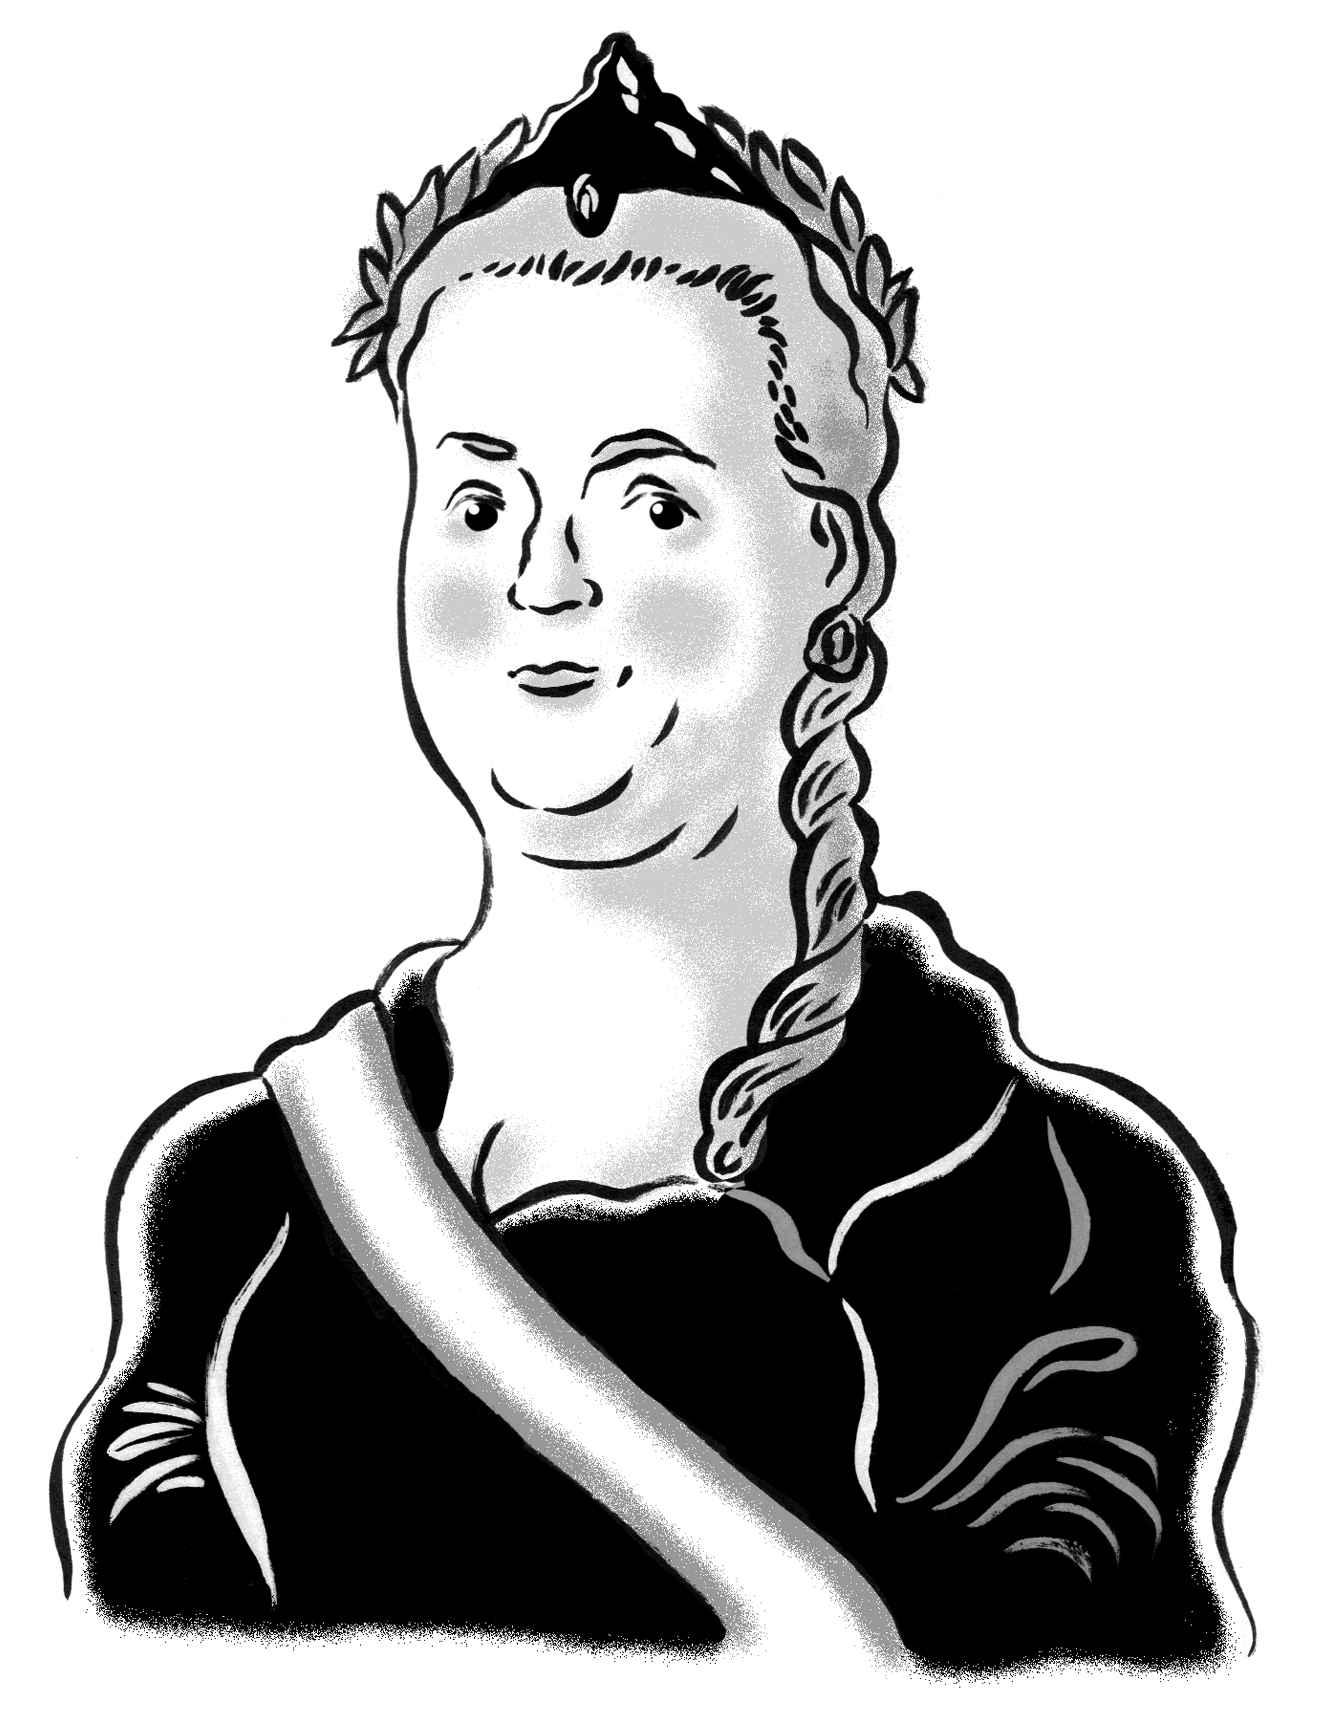
\includegraphics[width=6cm]{./imgs/autor1.jpg}
\end{center}

\chapter{Conto do tsarévitche Cloro}

\textls[-13]{Antes dos tempos de Kii, príncipe de Kiev,\footnote{Kii, rei lendário,
  um dos três irmãos criadores de Kiev (cidade"-mãe que deu origem à
  Rússia, hoje capital da Ucrânia), cuja fundação é datada do séc. \textsc{vi},
  conforme \emph{Narrativa dos Tempos Passados}.} vivia na Rússia um
tsar, um homem bom que amava a verdade e queria o bem de todos:
frequentemente percorria sua região para ver como as pessoas viviam e se
informava por toda parte se praticavam a verdade.}

O tsar tinha uma tsarina.\footnote{Tsar, tsarina, tsarévitche
  (aportuguesamento de \emph{tsariévitch}), nomes dados na Rússia,
  respectivamente, para rei, rainha e príncipe"-herdeiro.} Tsar e tsarina
viviam em concórdia; ela o acompanhava nas viagens e não gostava de
estar separada dele.

Uma vez, o tsar e a tsarina chegaram a uma cidade construída em uma
montanha alta, no meio de uma floresta. Lá nasceu o filho do tsar, de
beleza admirável, a quem deram o nome de Cloro; mas, durante os três
dias alegres de festejos, o tsar recebeu a notícia desagradável de que
seus vizinhos estavam agitados, tinham entrado em suas terras e cometido
diversas ofensas contra os moradores da fronteira. Ele reuniu as tropas
que estavam perto do acampamento e foi com elas defender as divisas. A
tsarina partiu com o marido. O tsarévitche ficou na cidade, na casa em
que nasceu. O pai designou"-lhe sete babás sábias e hábeis na educação de
crianças. Já a cidade, o tsar a mandou fortificar com uma muralha de
pedra bruta, com torres nos cantos, segundo o antigo costume; canhões
nas torres não colocaram, pois naquela época não havia quem tivesse
canhões. A casa em que o tsarévitche Cloro ficou morando, embora não
fosse construída com mármore da Sibéria e pórfiro, era muito boa e
confortável; na parte de trás havia jardins com árvores frutíferas,
junto aos quais abriram lagoas com peixes que enfeitavam o local; os
caramanchões de estilos de vários povos, de onde a vista se estendia ao
longe pelos campos e vales das redondezas, faziam da residência um lugar
muito agradável para se morar.

Quando o tsarévitche começou a crescer, a ama de leite e as babás
repararam que ele era tão inteligente e vivo como belo, e por toda parte
se espalharam rumores sobre a beleza, a inteligência e os bons talentos
do tsarévitche. Ouviu falar disso um cã\footnote{Cã (\emph{Khan}),
  título de chefe disseminado, durante a dominação mongol na Ásia (séc.
  \textsc{xii/xiii}), por várias regiões (sultões e reis o adotavam). Aqui foi
  usado pela imperatriz de forma anacrônica.} quirguiz, que errava
pela estepe selvagem de carruagem coberta; teve curiosidade de ver a
criança tão maravilhosa e, ao vê"-la, quis levá"-la consigo para a estepe.
Pôs"-se a pedir às babás que viajassem com o tsarévitche para o acampamento
dele; as babás disseram, com todo o respeito, que não podiam fazer nada
sem a permissão do tsar, que não tinham a honra de conhecer o senhor cã
e que não visitariam gente desconhecida na companhia do tsarévitche. O
cã não ficou satisfeito com essa resposta respeitosa, tornou"-se mais
insistente, como um faminto querendo pão, e pedia e pedia que as babás e
a criança fossem com ele até a estepe. Tendo recebido uma recusa firme,
entendeu finalmente que com rogos não alcançaria seu intento e lhes
mandou presentes. Agradecendo, elas devolveram as oferendas e mandaram
dizer que não precisavam de nada. O cã era teimoso e, firme em sua
intenção, pensou no que fazer. Passou"-lhe pela cabeça vestir roupas
gastas, sentar"-se ao portão do jardim, como se fosse um velho doente, e
pedir esmola aos passantes. Nesse dia, o tsarévitche, ao passear pelo
jardim, viu o velho sentado no portão e ordenou que descobrissem quem
era. Correram e foram saber quem podia ser. Voltaram com a resposta de
que era um mendigo doente. Cloro, uma criança curiosa, pediu para olhar
o homem doente; as babás contiveram o tsarévitche, dizendo que ali não
havia nada para ver e que mandasse uma esmola. O menino quis dar o
dinheiro sem ajuda de ninguém e saiu correndo na frente, e as babás
saíram atrás; mas, quanto mais rápido elas corriam, mais ele acelerava o
passo. Cloro atravessou correndo o portão e, quando se aproximou do
falso mendigo, prendeu o pé em um pedregulho e deu de cara com o chão; o
homem levantou"-se num pulo, pegou a criança nas mãos e lançou"-se com ela
morro abaixo. Lá o esperava uma pequena carruagem dourada, coberta de
veludo; ele entrou nela e partiu com o tsarévitche para a estepe. As
babás, ao chegarem ao portão, já não encontraram nem mendigo nem
criança, não viram nem vestígio deles, nem mesmo o caminho pelo qual o
cã desceu o morro, segurando o tsarévitche com uma mão, como uma galinha
pela asa, agitando o chapéu acima da cabeça com a outra mão e gritando
três vezes ``hurra''. Ao ouvir sua voz, as babás dispararam até o
declive, mas era tarde, não conseguiram alcançá"-los. O cã levou Cloro
sem atropelos ao seu acampamento nômade e entrou com a criança numa
tenda, onde foi recebido por seus dignitários. O cã confiou o
tsarévitche a seu melhor oficial; este tomou Cloro pela mão e conduziu"-o
a uma tenda ricamente enfeitada, revestida de damasco vermelho chinês e
tapetes persas. Ali colocaram o menino em uma almofada de brocados e se
puseram a consolá"-lo; mas ele chorava muito, lamentando ter fugido tão
rápido das babás, e perguntava sem parar para onde o tinham levado, por
quê, para quê. O oficial e os chefes quirguizes que estavam lá contaram
a ele muitas lorotas; um dizia que tudo tinha sido determinado pelas
estrelas, outro que era melhor viver lá do que em casa, disseram tudo,
menos a verdade, mas, ao ver que nada continha as lágrimas de Cloro,
pensaram em assustá"-lo com uma invencionice: ``Pare de chorar, senão
transformaremos você num morcego ou num milhafre, daí um lobo ou um sapo
irá comê"-lo''. O tsarévitche não era medroso e riu, entre lágrimas,
desse absurdo. O oficial, ao ver que a criança parara de chorar, mandou
arrumarem a mesa; com a mesa arrumada, trouxeram os pratos e o
tsarévitche comeu, no fim da refeição ofereceram geleia e todas as
frutas que tinham; depois do jantar, despiram o menino e o colocaram
para dormir.

No outro dia, antes de clarear, o cã reuniu seus dignitários e lhes
disse o seguinte: ``Como deve ser do conhecimento de vocês, ontem trouxe
comigo o tsarévitche Cloro, criança de rara beleza e inteligência.
Desejo saber com precisão se é verdade o que eu ouvira falar dele; para
conhecer seus talentos, pretendo empregar métodos variados''. Os
dignitários, ao ouvirem as palavras do cã, fizeram"-lhe reverências
profundas; os bajuladores louvaram"-lhe a atitude de ter raptado o filho
de outra pessoa, que, ainda por cima, era um rei vizinho; os medrosos
consentiram, dizendo: ``Amado soberano, como podia ser de outra forma se
é o que havia no seu coração?''. Alguns deles, os que realmente gostavam
do cã, menearam a cabeça e, quando ele perguntou por que estavam
calados, disseram com franqueza: ``Fez mal em raptar o filho do rei
vizinho e não iremos escapar da desgraça se você não emendar a sua
conduta''. O cã replicou: ``Vocês estão sempre se queixando de mim'',
não os levou em conta e, quando a criança acordou, mandou que a levassem
até ele. O tsarévitche, percebendo que queriam carregá"-lo, disse: ``Não
se deem o trabalho, sei andar, vou sozinho'', e entrou na tenda do cã,
fazendo reverências a todos --- ao cã em primeiro lugar, depois aos que
estavam à direita e à esquerda ---, em seguida se postou na frente do
soberano com um ar tão respeitoso, recatado e decoroso, que deixou não
apenas ele, mas todos os quirguizes admirados. Voltando a si, o cã disse
o seguinte: ``Tsarévitche Cloro, dizem que você é uma criança
inteligente; faça o favor de encontrar para mim uma rosa sem espinhos,
que não pique; o aio lhe mostrará um campo amplo, dou"-lhe o prazo de
três dias''. A criança fez uma reverência ao cã, disse ``sim, senhor'',
saiu da tenda dele e foi para a sua.

No caminho, deparou"-se com a filha do cã, que era casada com o sultão
Rabugento. Ele nunca ria e se zangava com os outros por rirem, enquanto
a esposa era de temperamento alegre e muito amável; ao ver Cloro, ela
disse: ``Salve, tsarévitche, como tem passado? Para onde vai?''. O
tsarévitche disse que, por ordem do cã, pai dela, ia procurar uma rosa
sem espinhos, que não picasse. A filha do cã, que se chamava Felícia,
espantou"-se por mandarem uma criança buscar uma coisa tão difícil de se
encontrar e, afeiçoando"-se ao menino sinceramente, disse: ``Tsarévitche,
espere um pouquinho, vou procurar com você uma rosa sem espinhos, que
não pique, se meu pai autorizar''. Cloro foi almoçar em sua tenda, pois
estava na hora, e Felícia foi pedir ao soberano permissão para ir
procurar uma rosa sem espinhos, que não picasse, na companhia do
tsarévitche. Não é que o cã apenas não tivesse permitido, ele proibiu
severamente que ela fosse procurá-la com a criança.

Felícia, após sair da tenda do pai, convenceu o marido, o sultão
Rabugento, a ficar com o cã, enquanto ela foi até o tsarévitche. O
menino alegrou"-se ao vê"-la e pediu que se sentasse ao seu lado, com o
que ela concordou e então disse: ``O cã não me deixou ir com você,
tsarévitche, procurar uma rosa sem espinhos, que não pique; mas lhe
darei um conselho bom, meu pequeno, e você deve se lembrar dele; escute
o que lhe direi e não esqueça''. O tsarévitche prometeu não esquecer.
``A certa distância daqui'', continuou ela, ``quando você for buscar uma
rosa sem espinhos, que não pique, encontrará pessoas de trato muito
agradável que tentarão convencê"-lo a ir com elas; irão lhe contar muitas
histórias alegres e dizer que gastam o tempo em diversões intermináveis;
não acredite nelas, são mentirosas, suas alegrias são falsas, com muito
tédio misturado. Depois delas, virão outras, que pedirão com mais fervor
a sua companhia; você recusará com firmeza e elas irão largá"-lo. Então
você entrará na floresta, onde encontrará gente lisonjeira, que se
esforçará de todas as formas, com conversas agradáveis, para desviá"-lo
do caminho verdadeiro; mas não se esqueça de que deve encontrar uma
única flor, uma rosa sem espinhos, que não pique. Gosto de você e
mandarei ao seu encontro meu filho, para ajudá"-lo a procurá"-la.'' Cloro,
após ouvir a fala de Felícia, disse: ``Mas será tão difícil encontrar
uma rosa sem espinhos, que não pique?''. ``Não'', respondeu a filha do
cã, ``não é especialmente difícil, desde que você seja sincero e tenha
firmeza na boa intenção.'' O menino perguntou se alguém já tinha
encontrado essa flor. ``Já vi'', disse Felícia, ``comerciantes e
camponeses que tiveram tanto êxito nisso como dignitários, tsares e
tsarinas.'' Após dizer isso, a filha do cã se despediu do tsarévitche; o
aio oficial conduziu o menino para que este fosse buscar a flor, passando"-o para o outro lado da cancela, onde
havia um bosque imenso, a reserva de animais do cã. Lá, Cloro viu diante
de si muitos caminhos: uns eram retos, outros curvos, outros se
cruzavam. A criança não sabia, no começo, por qual ir; ao ver um jovem
vindo em sua direção, apressou"-se em perguntar"-lhe quem era. O jovem
respondeu: ``Eu sou Juízo, filho de Felícia; minha mãe me mandou ir
procurar com você uma rosa sem espinhos, que não pique''. O tsarévitche,
agradecendo de coração à Felícia, tomou"-o pela mão e perguntou por que
caminho ir. Juízo, com ar alegre e audaz, disse: ``Não tema,
tsarévitche, vamos pelo caminho reto, que nem todos seguem, embora seja
mais belo que os outros''. ``Por que não o seguem?'', perguntou Cloro.
``Porque'', disse o jovem, ``param nos outros caminhos ou se perdem.''
Em marcha, o jovem mostrou uma trilha maravilhosa, dizendo: ``Veja,
tsarévitche, esse caminho é para as almas de crianças caridosas; é um
caminho bom e também curto''.

Passaram através da floresta e chegaram a um vale agradável, onde viram
um riacho de águas cristalinas com jovens ao lado; uns estavam sentados
na grama, outros deitados debaixo de árvores. Assim que viram o
tsarévitche, levantaram"-se e se aproximaram; um deles disse, com
respeito e cortesia: ``Permita"-me perguntar, senhor, aonde vai? Veio
parar aqui por acaso? Não podemos ter o prazer de lhe servir em algo?
Seu olhar já nos enche de reverência e amizade, e ficamos contentes ao
ver suas qualidades tão admiráveis''. Lembrando"-se das palavras de
Felícia, Cloro sorriu e disse: ``Não tenho a honra de conhecê"-lo, nem o
senhor me conhece, de modo que atribuo suas palavras unicamente ao
hábito da cortesia mundana, e não a meus méritos; estou em busca de uma
rosa sem espinhos, que não pique''. Outro dos que ali estavam
intrometeu"-se na conversa: ``Sua intenção demonstra seus grandes
talentos; mas faça uma gentileza a nós, fique conosco alguns dias que
seja e participe de nossas alegrias sem par''. O menino disse que tinha
um prazo a cumprir e não havia tempo para parar; ele temia a ira do cã.
Tentaram persuadi"-lo, dizendo que o descanso era necessário para a
saúde, que não encontraria lugar melhor ou mais adequado, nem gente mais
zelosa; queriam porque queriam convencê"-lo a ficar com eles. Por fim,
homens e mulheres, dando"-se as mãos, fizeram um círculo ao redor de
Cloro e seu guia, começaram a dançar e a pular, sem deixá"-los prosseguir; mas, enquanto rodopiavam, Cloro tomou Juízo pela mão e saiu
correndo tão rápido da roda, que não puderam contê"-lo. Adiante,
encontraram o Murzá\footnote{Murzá, título de nobreza feudal entre
  tártaros.} Preguiça, principal vigia daquele lugar, que passeava com
sua gente. Ao ver Cloro e seu guia, recebeu"-os com carinho e pediu que
entrassem em sua casa; os dois, um pouco cansados, foram até lá. Após
entrarem, o anfitrião os acomodou em um divã e se sentou ao lado, em
almofadas de pluma cobertas de brocado antigo; já as pessoas de casa
sentaram"-se junto às paredes. Depois o Murzá Preguiça ordenou que
trouxessem cachimbos para fumar e café. Ao ouvir que não fumavam
cachimbo e não bebiam café, mandou borrifar os tapetes com perfumes
inebriantes e perguntou a Cloro o motivo de sua vinda à reserva de
animais do cã. O tsarévitche respondeu que, por ordem do soberano,
buscava uma rosa sem espinhos, que não picasse. O anfitrião espantou"-se
com o fato de uma tarefa daquelas ser empreendida por alguém de tão
pouca idade, dizendo: ``Mesmo gente mais velha do que você não
conseguiu; descanse, não vá em frente, aqui há pessoas que tentaram
encontrar, mas, cansadas, desistiram''. Um dos que estavam sentados
levantou"-se e falou: ``Eu quis ir mais de uma vez, mas me aborreci e, no
lugar disso, fiquei morando com meu benfeitor, o Murzá Preguiça, que me
deixa beber e comer aqui''. No meio da conversa, o Murzá baixou a cabeça
e adormeceu. Quando os que estavam encostados nas paredes ouviram"-no
roncar, levantaram"-se devagarinho --- uns foram se arrumar e se
enfeitar, outros foram se deitar, outros deram de dizer fanfarrices,
outros pegaram cartas e dados. Durante todas essas atividades, uns se
zangavam, uns se alegravam, mas os rostos de todos refletiam seus
movimentos interiores. Quando o Murzá Preguiça acordou, voltaram a se
reunir ao seu redor, levando ao cômodo uma mesa com frutas. O Murzá
ficou no meio das almofadas felpudas e de lá ofereceu as frutas ao
tsarévitche, que reparava com muita atenção em tudo o que se passava.
No momento em que Cloro tentou experimentar o que lhe era servido, seu guia, Juízo,
segurou"-o de leve pela manga; o maravilhoso cacho de uvas que o
tsarévitche estava segurando espalhou"-se pelo chão; voltando a si, ele
imediatamente se levantou e ambos escaparam do palácio.

A pouca distância dali, viram uma casa camponesa e alguns
hectares\footnote{\textls[-20]{No original, foi usada \emph{dessiatina,}
  antiga medida russa para superfícies agrárias equivalente a 1,09
  hectare. Todas as ocorrências do termo foram adaptadas.}} de terra
bastante fecunda onde crescia todo tipo de cereais: centeio, aveia,
cevada, trigo"-sarraceno, etc. Tinham semeado os grãos; uns estavam
maduros, outro mal saíam da terra. Adiante, avistaram prados em que
pastavam ovelhas, vacas e cavalos. Encontraram o dono de regador na mão:
regava os pepinos e os repolhos cultivados pela esposa; os filhos
estavam trabalhando em outro lugar, arrancando erva daninha das
verduras. Juízo disse: ``Deus abençoe, boa gente''; eles responderam:
``Obrigado, patrão''. Fizeram uma reverência ao tsarévitche
desconhecido, mas pediram amigavelmente a Juízo: ``Visite, por favor,
nossa morada, e a filha do cã, sua mãe, terá pena de nós, nos visitará e
não nos abandonará''. Juízo concordou em ir à casa deles e, seguido de
Cloro, foi até o quintal. No meio havia um carvalho vetusto e alto e,
embaixo dele, um banco largo e limpo com uma mesa na frente. Os
visitantes sentaram"-se no banco, a anfitriã e sua nora esticaram uma
toalha na mesa e colocaram uma tigela com coalhada e outra com ovos
fritos, um prato com panquecas quentes e ovos cozidos, e, no centro, um
belo presunto; puseram pão de farinha fina e, ao lado de cada um, um
pote de leite, e depois, com os petiscos, trouxeram favos e pepinos
frescos e oxicoco com mel. O anfitrião pediu: ``Comam, façam o favor''.
Os viajantes, que estavam famintos, não recusaram nada e, enquanto isso,
conversaram com o anfitrião e a anfitriã, que lhes contaram como viviam
bem, alegres e tranquilos, e como estavam satisfeitos com sua situação,
tendo passado a vida em tarefas do campo e superando com trabalho árduo
toda necessidade e carência. Depois do jantar, estenderam um feltro no
mesmo banco: Cloro e Juízo colocaram suas capas em cima dele e, depois de a anfitriã
trazer um travesseiro com uma fronha branca para cada, eles se deitaram
e, de tão cansados, dormiram profundamente.

%\thisfloatpagestyle{empty}
\begin{figure}%[ht!]
\vspace*{-2.2cm}
\hspace*{-2.3cm}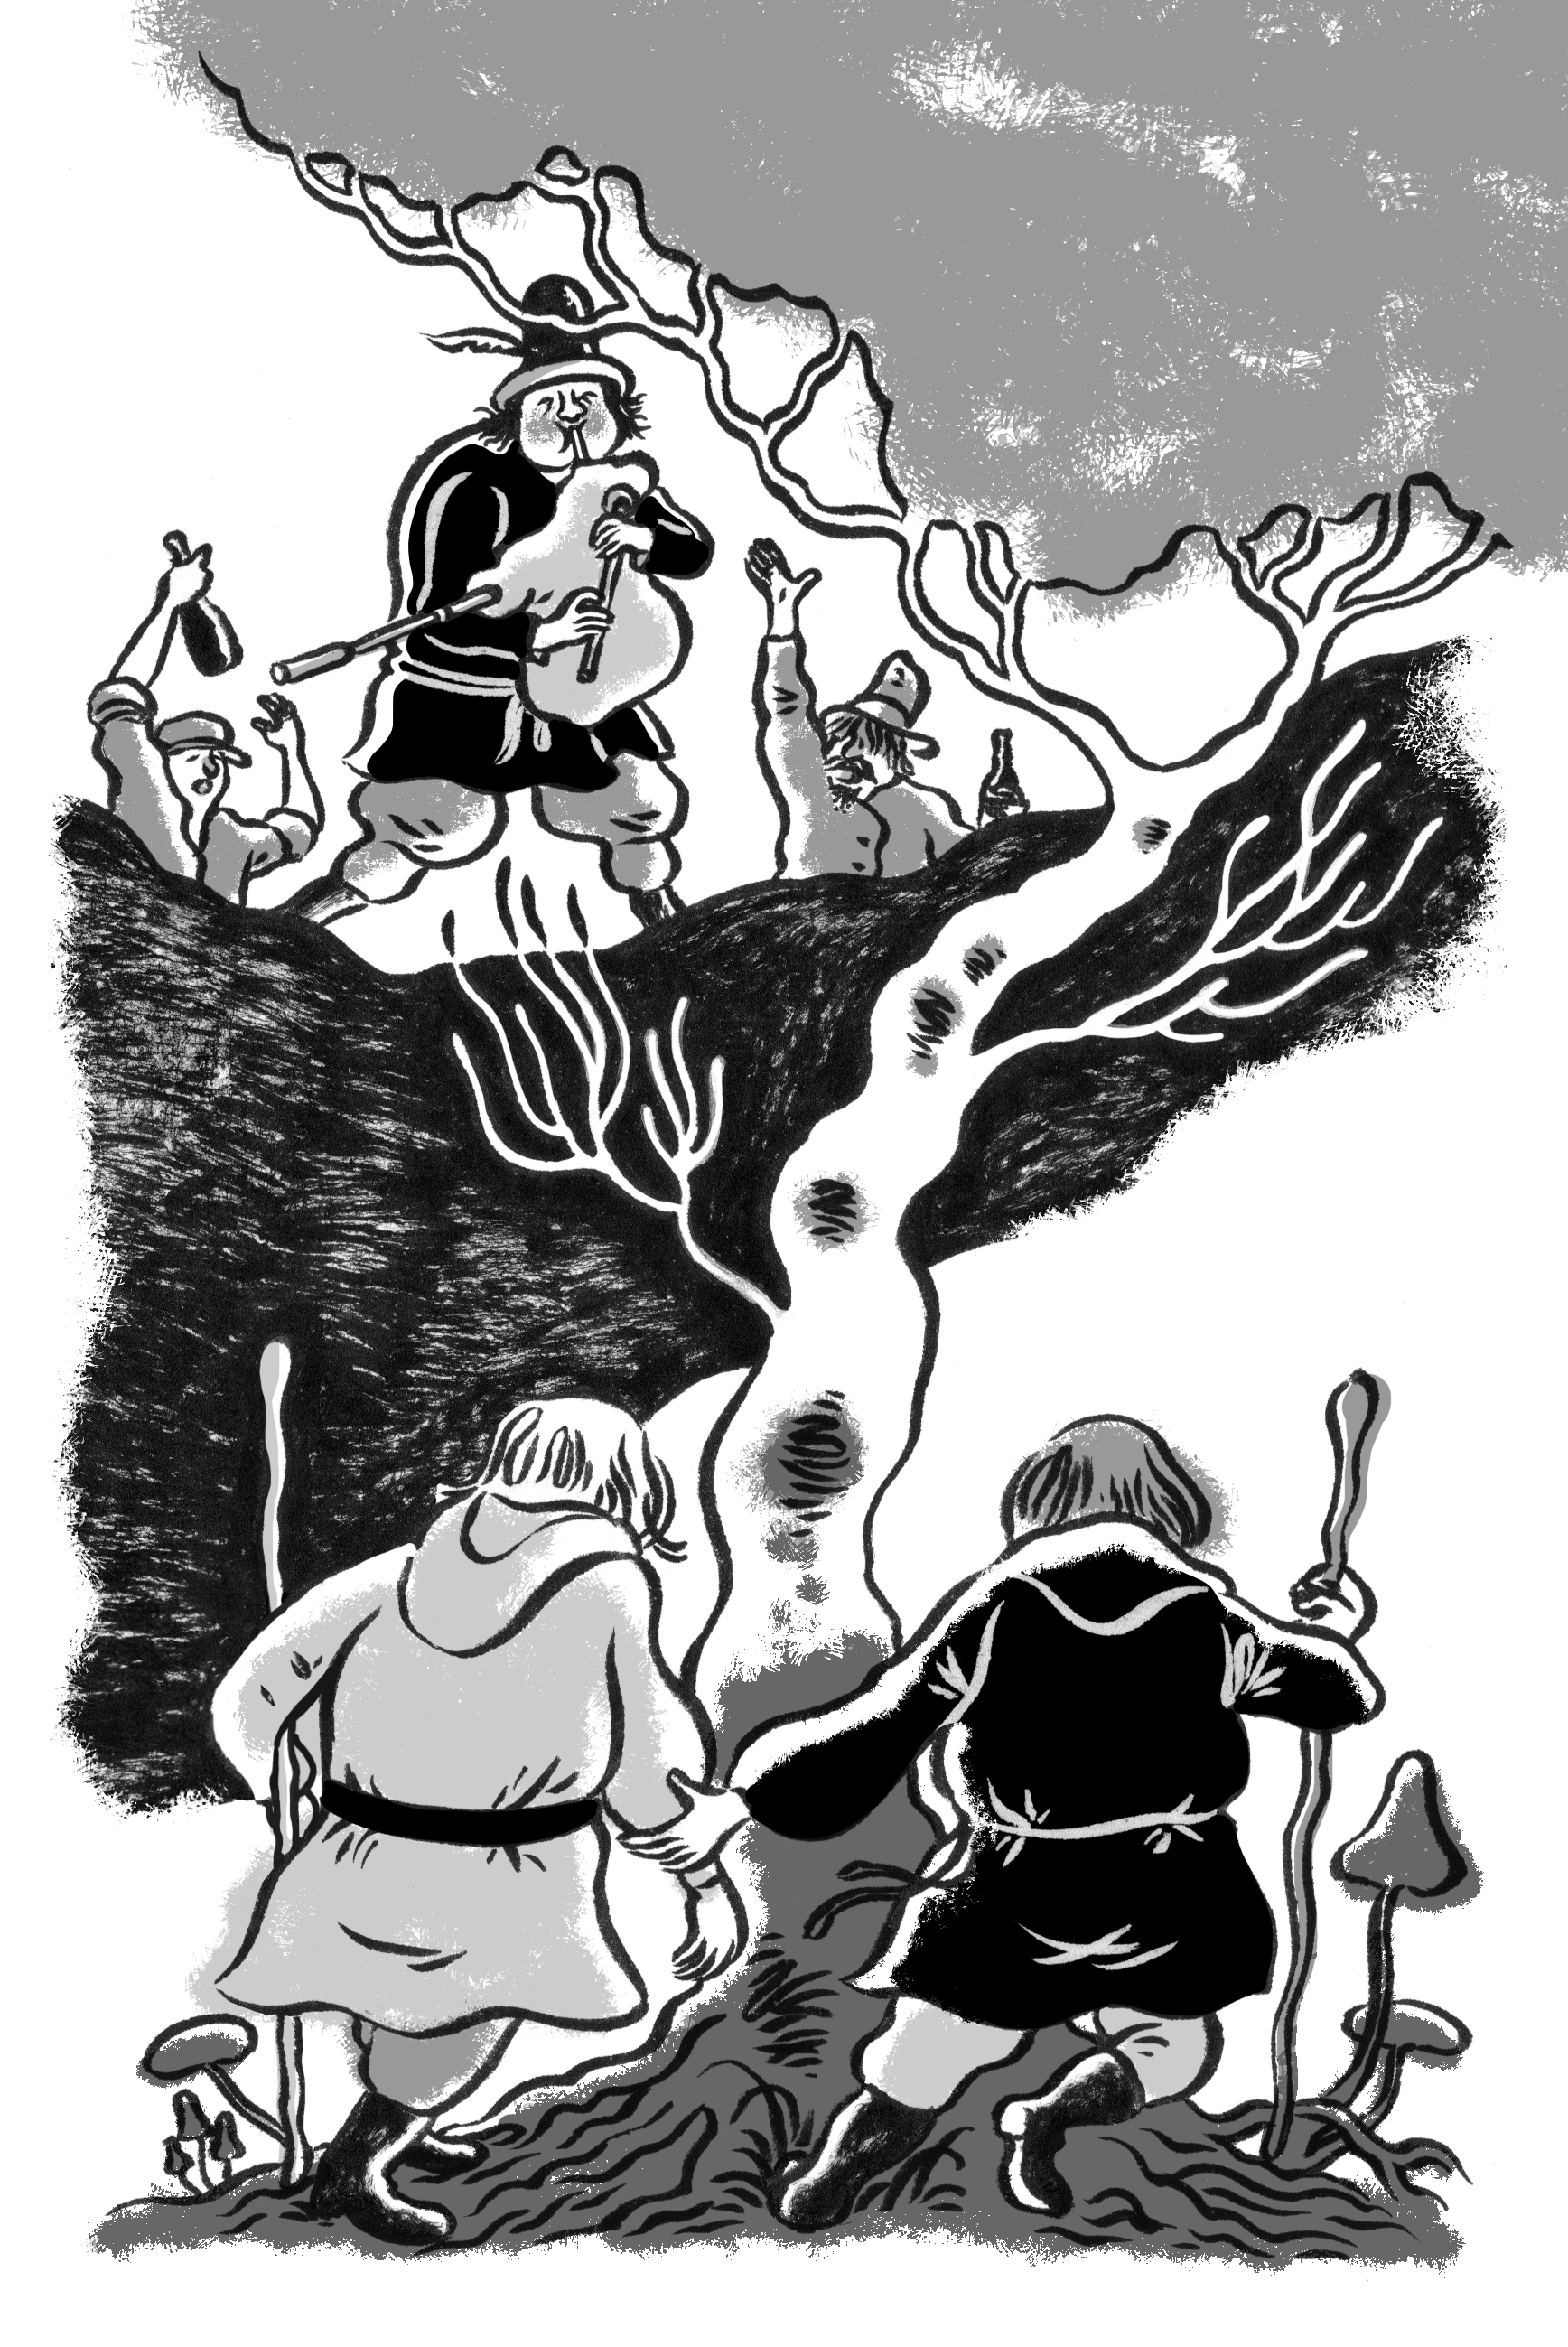
\includegraphics{./imgs/cena1.jpg}
\end{figure}

Despertaram com o nascer do dia, agradeceram ao anfitrião, que não quis
aceitar nada pelo pernoite, e se puseram a caminho. Após percorrerem
meio quilômetro,\footnote{No original, foi usada \emph{verstá,} antiga
  medida russa para distâncias equivalente a 1,067km. Todas as
  ocorrências do termo foram adaptadas.} ouviram ao longe uma gaita de
foles. Cloro quis se aproximar, mas Juízo tentou persuadi"-lo, dizendo
que a gaita os afastaria do caminho. Tomado pela curiosidade, o
tsarévitche aproximou"-se da gaita de foles, porém, ao ver as
barbaridades que os bêbados faziam em volta do gaiteiro, assustou"-se e
se lançou nos braços de Juízo. Este voltou a colocá"-lo no caminho reto,
onde, após passarem pela mata, avistaram uma subida íngreme. O guia disse
ao tsarévitche que lá crescia a rosa sem espinhos, que não picava. Daí
Cloro sentiu o calor do sol e ficou cansado; começou a se aborrecer,
disse que aquele caminho não tinha fim, perguntou se demoraria muito, se
não podiam ir por outro. Juízo respondeu que o levava pelo caminho mais
curto e que só a paciência supera as dificuldades. O tsarévitche, com
insatisfação, replicou: ``Então vou procurar outro caminho sozinho'', e,
abanando o braço em sinal de desaprovação, acelerou o passo e afastou"-se
do guia.

Juízo ficou para trás e o seguia calado, em passo silencioso. Cloro
enfiou"-se em um vilarejo, no qual mal olharam para ele, pois era dia de
negociar e todos estavam ocupados com regateios e trocas na praça do
mercado. Andando por entre as telegas,\footnote{Telega, carroça de carga
  usada na Rússia puxada por cavalos.} no burburinho do mercado, o
tsarévitche começou a chorar. Um sujeito que não o conhecia passou a seu
lado e, ao ver uma criança chorando, disse: ``Pare de berrar, fedelho,
sem isso aqui já é barulhento o suficiente''. Juízo alcançou"-o bem nessa
hora; o menino se queixou do homem que o ofendera. Juízo, sem dizer uma
palavra, tirou"-o de lá; quando Cloro perguntou por que ele não estava
lhe falando como antes, o guia disse: ``Você não pediu meus conselhos,
meteu"-se sozinho nesse lugar indecente, então não fique bravo se
encontrar pessoas ou discursos que não condizem com suas ideias''. Ele
quis continuar a fala, mas toparam com um homem que não era novo, porém
tinha aspecto agradável, cercado de muitos jovens. Cloro, sempre
curioso, chamou um deles e perguntou quem era o homem. O jovem disse:
``É o nosso professor; terminamos a aula e vamos passear; e vocês, para
onde vão?''. O tsarévitche respondeu: ``Procuramos uma rosa sem
espinhos, que não pique''. ``Eu ouvi'', falou o jovem, ``do nosso
professor a explicação da rosa sem espinhos, que não pica; essa flor não
é nada além da virtude; uns pensam alcançá"-la por caminhos tortuosos,
mas ninguém a alcança fora do caminho reto; feliz daquele que, com
firmeza e pureza no coração, supera todas as dificuldades do trajeto.
Vejo sua montanha, onde cresce a rosa sem espinhos, que não pica, mas o
caminho é íngreme e rochoso.'' Após dizer isso, despediu"-se deles e foi
atrás de seu mestre.

Cloro e seu guia dirigiram"-se à montanha e encontraram uma trilha
estreita e rochosa, pela qual andaram com dificuldade. Daí se depararam
com um velho e uma velha vestindo roupas brancas, ambos de ar
respeitável; eles lhes estenderam seus cajados, dizendo: ``Apoiem"-se
neles e tentem não tropeçar''. Os que ali estavam disseram que o nome de
um era Honestidade e da outra Verdade.

Apoiados nos cajados, chegaram ao sopé da montanha e foram obrigados a
sair da trilha e a trepar num galho e, de galho em galho, alcançaram o
topo da montanha, onde encontraram a rosa sem espinhos, que não picava.
Mal a tiraram do arbusto, soaram trombetas e timbales na catedral dos
arredores, e por toda parte correu o rumor de que o tsarévitche Cloro,
tão novo, encontrara a rosa sem espinhos, que não picava. Ele apressou"-se
em levar a flor até o cã, e o cã mandou Cloro e a flor para o tsar. Este
ficou tão contente com a chegada do tsarévitche e com seus êxitos, que
se esqueceu de toda angústia e tristeza por que tinha passado. O
tsarévitche, o tsar, a tsarina e todas as pessoas do reino se amavam
mais a cada hora e por isso a cada hora a virtude se fortalecia entre eles. Aqui
acaba a história e quem souber que conte outra.\enlargethispage{\baselineskip}

%\medskip

{\footnotesize\hfill\emph{Tradução: Irineu Franco Perpetuo.}}

\chapter*{}
\label{part2}
\thispagestyle{empty}

\begin{vplace}[1.5]
{\HUGES\hfill\textbl{VLADÍMIR ODÓIEVSKI}}

{\LARGE\hfill\textlt(1803–1869)}
\end{vplace}

\pagebreak
\thispagestyle{empty}
\mbox{}
\vfill
\begin{center}
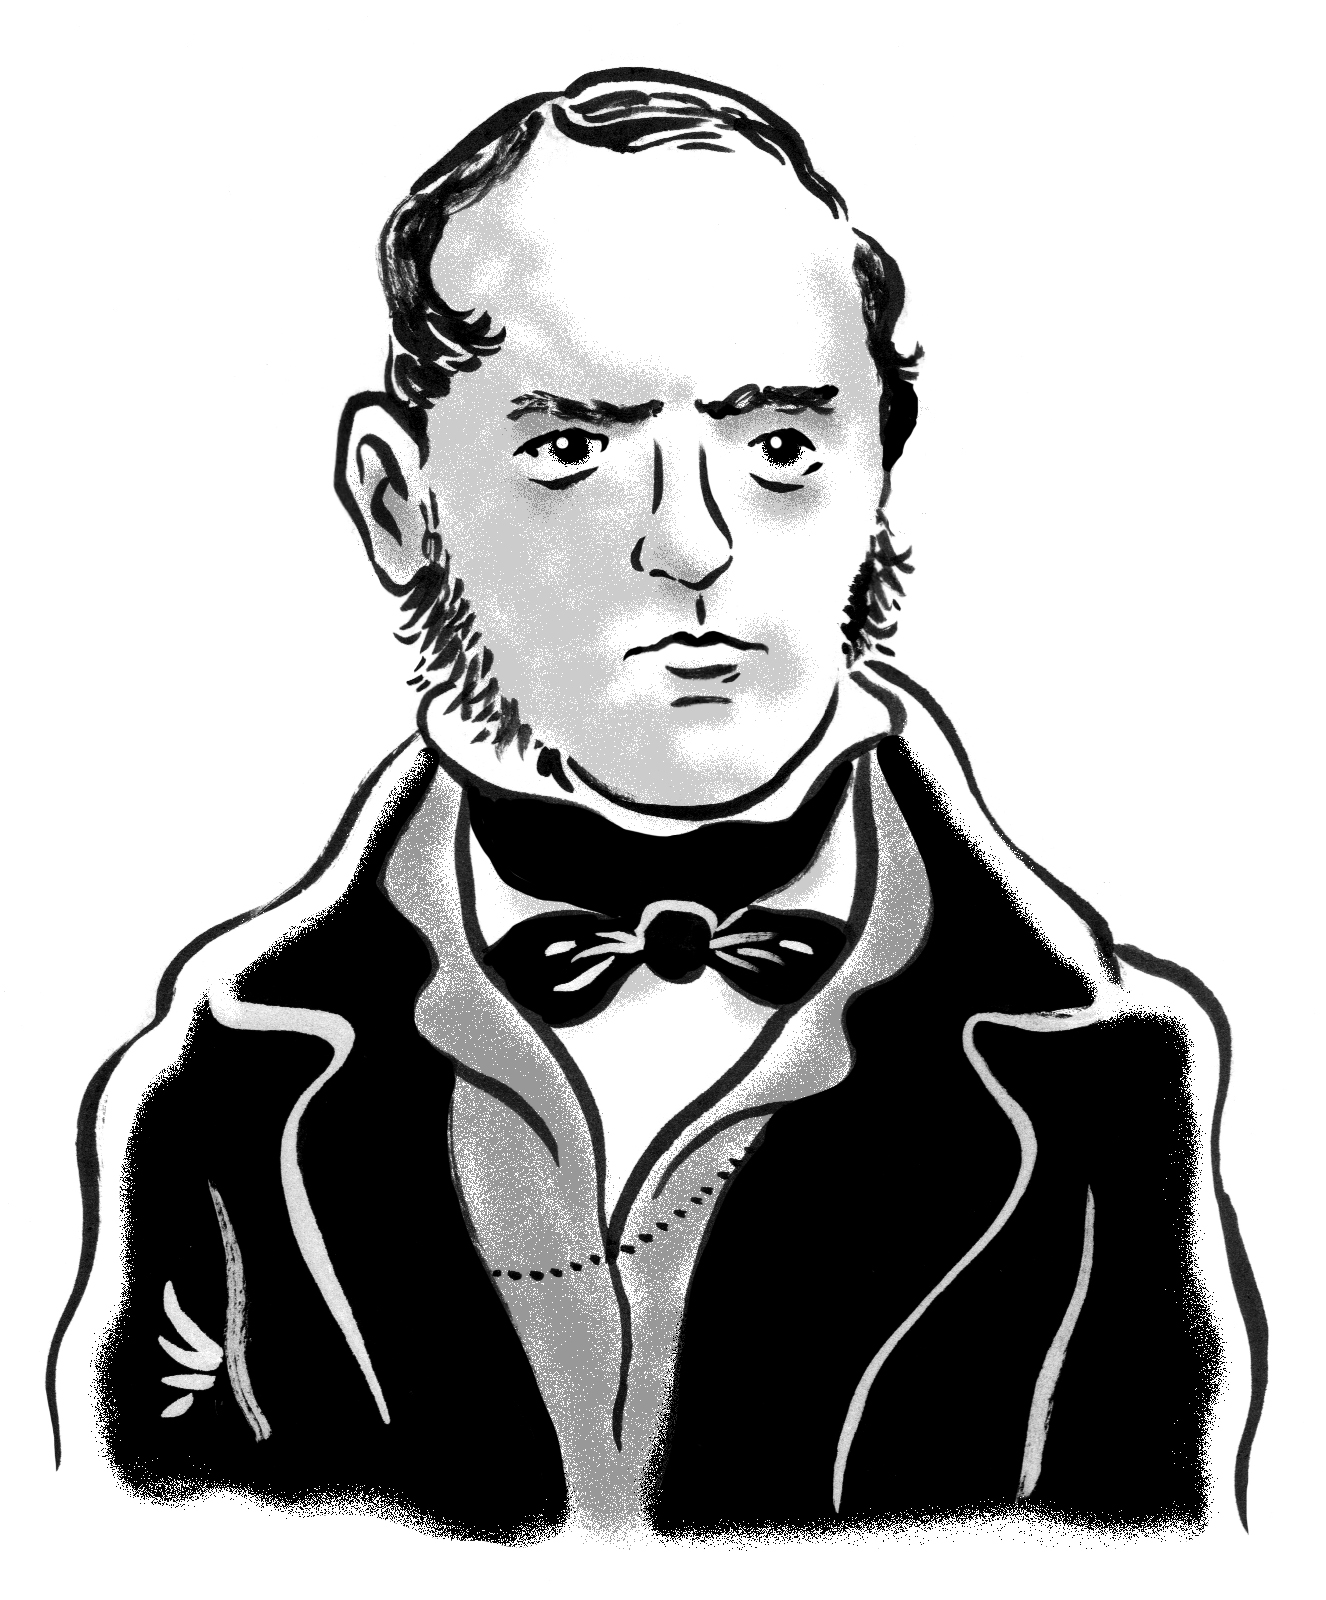
\includegraphics[width=6cm]{./imgs/autor2.jpg}
\end{center}


\chapter{A cidadezinha na tabaqueira}

O pai colocou uma tabaqueira na mesa.

--- Venha cá, Micha, dê uma olhada --- disse ele.

Мicha era um menino obediente, no mesmo instante largou os brinquedos e
foi até seu pai. E havia bem o que olhar! Que tabaqueira maravilhosa!
Colorida, de tartaruga. E a tampa era inacreditável! Portões, torres,
uma casinha, outra, mais uma, uma quarta, nem dava para contar, cada vez
menores, e todas de ouro; аs árvores também eram de ouro e suas folhas
de prata; detrás das árvores, erguia"-se um solzinho cujos raios rosados
espalhavam"-se por todo o céu.

--- Que cidadezinha é essa? --- perguntou Micha.

--- É a cidadezinha de Din"-din --- respondeu o pai e acionou uma
mola\ldots{}

E o que aconteceu? De repente, não se sabe de onde, começou a soar uma
música. De onde vinha essa música Micha não conseguia compreender; foi
até a porta --- não seria do outro quarto? E até o relógio --- não seria
de dentro do relógio? Foi até a escrivaninha, até a cristaleira; aguçou
o ouvido, olhou até debaixo da mesa\ldots{} Finalmente, convenceu"-se de
que a música estava vindo de dentro da tabaqueira. Aproximou"-se dela e
olhou --- o sol saiu detrás das árvores e andou de mansinho pelo céu, e
o céu e a cidadezinha iam ficando mais e mais claros; as janelas
brilhavam como fogo e as torres pareciam irradiar luz. Daí o solzinho,
cada vez mais baixo, foi para o outro lado do céu e, por fim,
desapareceu completamente atrás de uma colina, então a cidadezinha
escureceu, os contraventos se fecharam e as torres se apagaram, mas não
por muito tempo. Logo se acendeu uma estrelinha, depois outra, depois
uma lua com chifres surgiu por trás das árvores, a cidade voltou a ficar
clara e as janelinhas prateadas, e das torres saíam raios azulados.

--- Papai! Papai, posso entrar nessa cidadezinha? Como eu queria!

--- É difícil, meu amigo. Essa cidadezinha não é do seu tamanho.

--- Não tem problema, papai, sou pequeno. Só me deixe ir, eu queria
tanto saber o que acontece lá\ldots{}

--- Na verdade, meu amigo, lá já é apertado sem você.

--- Mas quem mora lá?

--- Quem mora lá? Lá moram sininhos.

Com essas palavras, o pai levantou a tampa da tabaqueira, e o que Micha
viu? Sininhos, martelinhos, um cilindro e rodas. O menino ficou admirado.

--- Para que estes sininhos? Para que os martelinhos? Para que o
cilindro com os ganchos? --- Micha perguntou ao seu pai.

E ele respondeu:

--- Não vou dizer, Micha. Observe com atenção e pense bem: talvez
adivinhe. Apenas não toque nessa mola, senão tudo quebrará.

O pai saiu e Micha ficou com a tabaqueira. Sentou na frente dela, olhou,
olhou, pensou, pensou: o que fazia os sinos soarem?

Enquanto isso, a caixinha de música da tabaqueira continuava a soar, só
que cada vez mais baixo, como se alguma coisa prendesse cada nota, como
se algo afastasse um som do outro. Daí Micha viu, debaixo da tabaqueira,
abrir uma portinhola e por ela sair correndo um menino de cabecinha
dourada e saiote de aço. Ele parou na soleira e chamou Micha com um
aceno.

``Mas por que'', pensou ele, ``papai disse que essa cidadezinha já é
apertada sem mim? Não, pelo visto tem gente boa morando lá; veja só,
estão me convidando para fazer uma visita.''

--- Obrigado, com imenso prazer.

Сom essas palavras, Micha correu até a portinhola e reparou com surpresa
que ela era exatamente do seu tamanho. Como um rapaz bem"-educado,
considerava que seu primeiro dever era dirigir"-se ao seu guia.

--- Com licença, gostaria de saber --- disse Micha --- com quem tenho a
honra de falar?

--- Din, din, din --- respondeu o desconhecido. --- Sou o
menino"-sininho, morador dessa cidade. Ouvimos dizer que você queria
muito nos visitar, por isso decidimos pedir"-lhe que nos conceda a honra
de ser nosso hóspede. Din, din, din, din, din, din.

Micha curvou"-se respeitosamente, o menino"-sininho tomou"-o pela mão e os
dois partiram. Então Micha notou que acima deles havia uma abóbada feita
de papel estampado de borda dourada. Na frente deles, havia outra
abóbada, só que menor; depois uma terceira, ainda menor; uma quarta,
ainda menor, e assim por diante; quanto mais para a frente, menores as
abóbadas ficavam, até que sob a última a cabecinha do guia mal passava.

--- Muito agradecido pelo convite --- disse Micha ---, mas não sei se
poderei aproveitar. É verdade que por aqui eu passo livremente, mas veja como lá as abóbadas são baixas; permita"-me falar com
franqueza, mas lá eu não passo nem me arrastando. Estou espantado por
você conseguir\ldots{}

--- Din, din, din --- respondeu o menino ---, vamos, não se preocupe,
apenas venha atrás de mim.

Мicha obedeceu. De fato, a cada passo as abóbadas pareciam se levantar,
e nossos meninos passaram livremente por todos os lugares; quando
chegaram à última abóbada, o menino"-sininho pediu a Micha que olhasse
para trás. Ele olhou, e o que viu? Agora a primeira abóbada, aquela por
onde passara ao entrar pela portinhola, parecia pequena, como se tivesse
encolhido. Micha ficou muito surpreso.

--- Como é possível? --- perguntou a seu guia.

--- Din, din, din --- respondeu o guia, rindo ---, de longe sempre
parece assim; pelo visto, você nunca olhou para nada com atenção: de
longe tudo parece pequeno e, quando você se aproxima, grande.

--- Sim, é verdade --- respondeu Micha ---, até agora não tinha me dado
conta disso, e veja só o que me aconteceu: anteontem, quis desenhar
mamãe tocando piano ao meu lado e papai lendo um livro na outra ponta da
sala. Só que não consegui fazer de jeito nenhum! Eu me esforcei para
valer, desenhei o mais fielmente possível, mas no papel sempre surgia
papai sentado ao lado da mamãe, com a poltrona dele ao lado do piano; só
que eu via muito bem que o piano estava perto de mim, junto da janela, e
papai estava sentado na outra ponta, perto da lareira. Mamãe me disse
que eu devia desenhar papai pequeno, mas achei que estava brincando,
pois ele é muito mais alto do que ela, mas agora estou vendo que disse a
verdade: eu tinha que ter desenhado papai pequeno, porque estava sentado
longe; fico muito agradecido pela explicação, muito agradecido.

O menino"-sininho morreu de rir.

--- Din, din, din, que engraçado! Din, din, din, que engraçado! Não sabe
desenhar papai e mamãe! Din, din, din, din, din!

Micha ficou chateado porque o menino"-sininho ria dele de forma tão
impiedosa e disse muito polidamente:

--- Permita"-me perguntar: por que, a cada palavra, você diz ``din, din,
din''?

--- É o nosso bordão --- respondeu o menino"-sininho.

--- Bordão? --- observou Micha. --- Papai diz que não é bonito usar
bordões.

O menino"-sininho mordeu a língua, não disse uma palavra.

Diante deles se abriram outras portinholas, e Micha viu"-se numa rua. Que
rua! Que cidadezinha! Calçada revestida de madrepérola; céu
multicolorido, de tartaruga; um sol dourado pairando; bastava
chamá"-lo com um aceno para que ele descesse, então rodopiava em volta de
sua mão e subia de novo. E casinhas de aço polido, tapadas por
conchinhas de diversas cores e, embaixo de cada tampa, sentava um
menino"-sininho de cabeça dourada, saiote prateado, e eram muitos, muitos
deles, um ficando menor do que o outro.

--- Não, agora não me enganam mais --- disse Micha ---, parecem menores
de longe, mas os sininhos são todos iguais.

--- Ah, não é verdade --- respondeu o guia ---, os sininhos não são
iguais. Se todos nós fôssemos iguais, um teria a mesma voz que o outro;
mas você não escuta os sons que tiramos? É que alguns de nós são maiores
e têm a voz mais grossa; por acaso você não sabia? Que isso lhe sirva de
lição, Micha: não ria de quem usa bordões; a pessoa pode usar bordões,
mas saber mais do que a outra e ter algo a ensinar.

Foi a vez de Micha morder a língua.

Enquanto isso, eles foram cercados por meninos"-sininhos, que puxavam a
roupa de Micha, tilintavam, saltitavam, corriam.

--- A vida de vocês é alegre --- disse Micha ---, eu ficaria com vocês
para sempre; não fazem nada o dia inteiro; não têm aula nem professor, e
ainda tocam música sem parar.

--- Din, din, din! --- gritaram os sininhos. --- Acha que somos alegres?
Não, Micha, nossa vida é ruim. É verdade que não temos aulas, mas de que
adianta? Não temos medo de aulas. Toda nossa desgraça (pobres de nós!)
está no fato de não termos o que fazer; de não termos livros nem
desenhos, nem pai nem mãe, nada que nos ocupe; o dia inteiro tocando e
tocando, e isso, Micha, é maçante, muito maçante! Nosso céu de tartaruga
é bonito, nosso solzinho dourado é bonito, as árvores douradas também,
mas, pobres de nós, já olhamos o bastante para eles, estamos fartos de
tudo isso; nunca pusemos os pés fora da cidade, e você pode imaginar o
que é passar a vida sem ter nada para fazer, dentro de uma caixinha de
música de uma tabaqueira?

--- Sim --- respondeu Micha ---, está dizendo a verdade. Isso também
acontece comigo: quando, depois das aulas, pego meus brinquedos, é
divertido; mas, quando, em um feriado, brinco o dia inteiro, fica
tedioso à noite; posso pegar um brinquedo, outro, nada é especial.
Fiquei muito tempo sem entender por que era assim, mas agora entendo.

--- Como se não bastasse, temos outra desgraça, Micha: temos bedéis.

--- Mas que espécie de bedéis?

--- Os bedéis"-martelinhos --- responderam os sininhos ---, como são
malvados! Vivem andando pela cidade e batendo na gente. Os maiores levam
menos toc"-toc, mas os pequenos apanham até doer.

De fato, Micha viu andando pela rua uns senhores narigudos de perninhas
finas resmungando entre si: toc"-toc"-toc! Toc"-toc"-toc! Levante, toque.
Toc"-toc"-toc! Toc"-toc"-toc!

De fato, os bedéis"-martelinhos faziam ora toc"-toc em um sininho, ora em
outro, sem cessar, até o coitado do Micha sentiu pena. Ele se aproximou
dos senhores, fez uma reverência muito cortês e perguntou com ar bondoso
por que eles martelavam os pobres meninos sem ter dó.

Os martelinhos respondiam:

--- Fora daqui, não atrapalhe! Lá na sala há um inspetor de roupão que
nos manda bater. Tudo gira e se encaixa. Toc"-toc"-toc! Toc"-toc"-toc!

--- Quem é o inspetor? --- Micha perguntou aos sininhos.

--- É o senhor Cilindro --- eles tilintaram ---, um homem bom em alto
grau. Fica dia e noite grudado no sofá. Não podemos nos queixar dele.

Micha foi até o inspetor. Viu que estava mesmo de roupão deitado no
sofá, girando de um lado para outro, porém sempre de cara virada para
cima. E, em seu roupão, havia pinos e ganchinhos a perder de vista;
quando aparecia um martelinho, o inspetor o encaixava num gancho e
depois o soltava, e o martelinho batia em um sininho.

\begin{figure}%[ht!]
\vspace*{-2.5cm}
\hspace*{-2.2cm}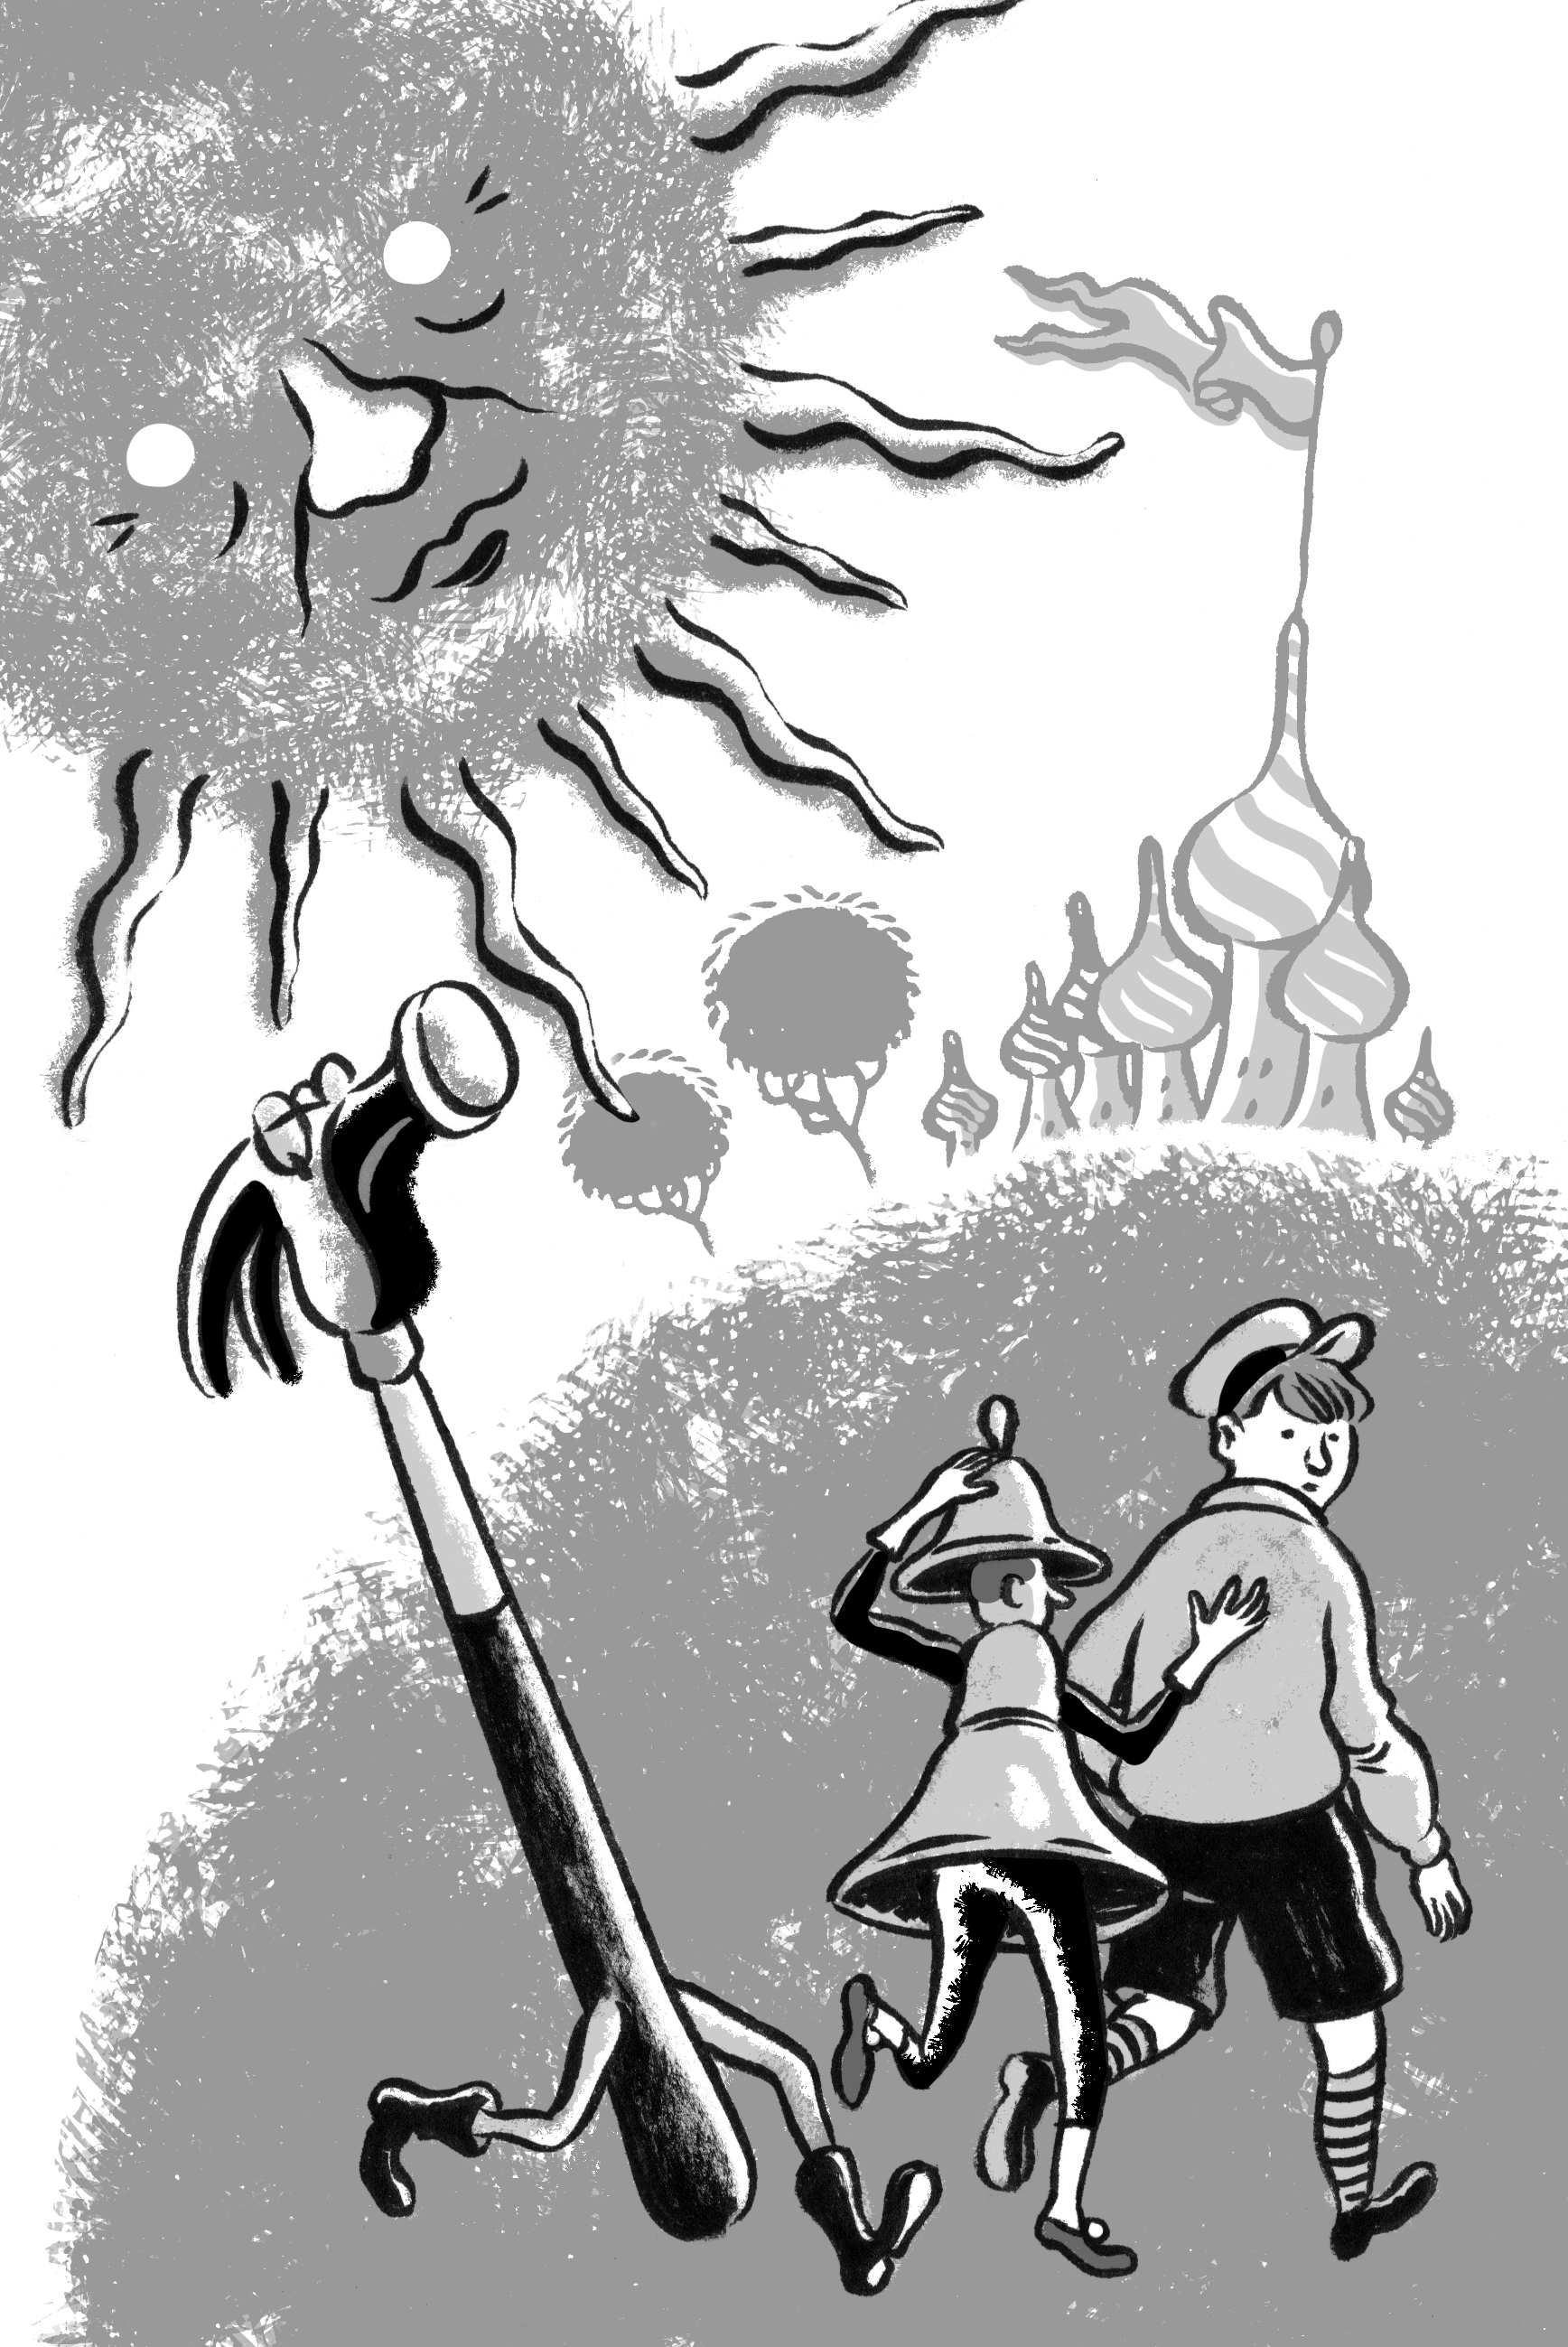
\includegraphics{./imgs/cena2.jpg}
\end{figure}

Assim que Micha se aproximou dele, o inspetor gritou:

--- Uni"-duni"-tê! Quem está andando por aqui? Quem está vagando por aqui?
Uni"-duni"-fora, quem não vai embora? Quem não me deixa dormir?
Uni"-duni"-tê! Uni"-duni"-tê!

--- Sou eu --- respondeu Micha, corajoso ---, eu, Micha\ldots{}

--- E o que deseja? --- perguntou o inspetor.

--- Tenho pena dos pobres meninos"-sininhos, são tão inteligentes, tão
bonzinhos, tão musicais e, por seu decreto, os bedéis batem neles sem
parar\ldots{}

--- Que tenho eu com isso, ora, ora? Eu não sou o maioral daqui. Que os
bedéis continuem batendo nos meninos! Que tenho eu com isso? Sou um
inspetor decente, fico deitado no sofá e não olho para ninguém\ldots{} Ora,
ora\ldots{}

--- Quem diria, aprendi muitas coisas nessa cidade! --- Micha disse
consigo mesmo. --- Às vezes fico aborrecido quando o inspetor não tira
os olhos de mim na escola! ``Que malvado'', penso eu. ``Afinal, ele não
é nem papai nem mamãe. Por que é da conta dele se eu faço travessuras?
Devia ficar em seu quarto.'' Não, agora estou vendo o que acontece com
os pobres meninos quando não há ninguém para cuidar deles.

Enquanto isso, Micha seguiu adiante e de repente parou. Viu uma tenda
dourada com uma franja de pérolas em cima da qual rodava, como um moinho
de vento, um cata"-vento dourado e, embaixo da tenda, estava deitada a
rainha"-mola, que, feito uma serpente, enrolava"-se e desenrolava"-se,
empurrando o flanco do inspetor sem parar. Micha ficou muito surpreso e
disse:

--- Senhora rainha! Por que fica empurrando o inspetor?

--- Zás, zás, zás --- respondeu a rainha ---, que menino desmiolado, que
menino tonto! Olha para tudo e não vê nada! Se eu não empurrasse o
cilindro, o cilindro não giraria; se o cilindro não girasse, não
encaixaria nos martelinhos; se os martelinhos não batessem, os sininhos
não tocariam; se os sininhos não tocassem, não haveria música! Zás, zás,
zás!

Micha teve vontade de saber se a rainha estava dizendo a verdade. Ele se
inclinou e apertou"-a com o dedinho --- e o que aconteceu? Em um instante
a mola desenrolou com força, o cilindro girou com força, os martelinhos
bateram rápido, os sininhos tocaram um disparate e, de repente, a mola
rebentou. Tudo se calou, o cilindro parou, os martelinhos caíram, os
sininhos tombaram de lado, o solzinho ficou pendurado, as casinhas se
quebraram. Então Micha se lembrou de que seu pai o mandara não tocar na
mola, assustou"-se e\ldots{} despertou.

--- Com que você sonhou, Micha? --- seu pai perguntou.

Micha demorou muito a recobrar os sentidos. Olhou em volta: era o quarto
do pai, a tabaqueira estava na sua frente; ao lado, seu pai e sua mãe
estavam sentados e riam.

--- Cadê o menino"-sininho? Cadê o bedel"-martelinho? Cadê a rainha"-mola?
--- perguntou Micha. --- Não passou de um sonho?

--- Sim, Micha, a música o embalou e você caiu no sono. Conte, pelo
menos, com que sonhou?

--- Sim, veja, papai --- disse Micha, esfregando os olhos ---, eu queria
saber como saía música da tabaqueira; comecei a olhar com atenção e a
examinar o que se mexia e como se mexia; pensei, pensei, e já estava
quase lá quando, de repente, vi a portinhola da tabaqueira se abrir\ldots{}
--- aí Micha contou todo o seu sonho.

--- Bem, agora estou vendo --- disse seu pai --- que você quase entendeu
por que sai música da tabaqueira; mas irá compreender mais quando for
estudar a mecânica.

\medskip

{\footnotesize\hfill\emph{Tradução: Irineu Franco Perpetuo.}}

\chapter*{}
\label{part3}
\thispagestyle{empty}

\begin{vplace}[1.5]
{\HUGES\hfill\textbl{IVAN TURGUÊNIEV}}

{\LARGE\hfill\textlt(1818–1883)}
\end{vplace}

\pagebreak
\thispagestyle{empty}
\mbox{}
\vfill
\begin{center}
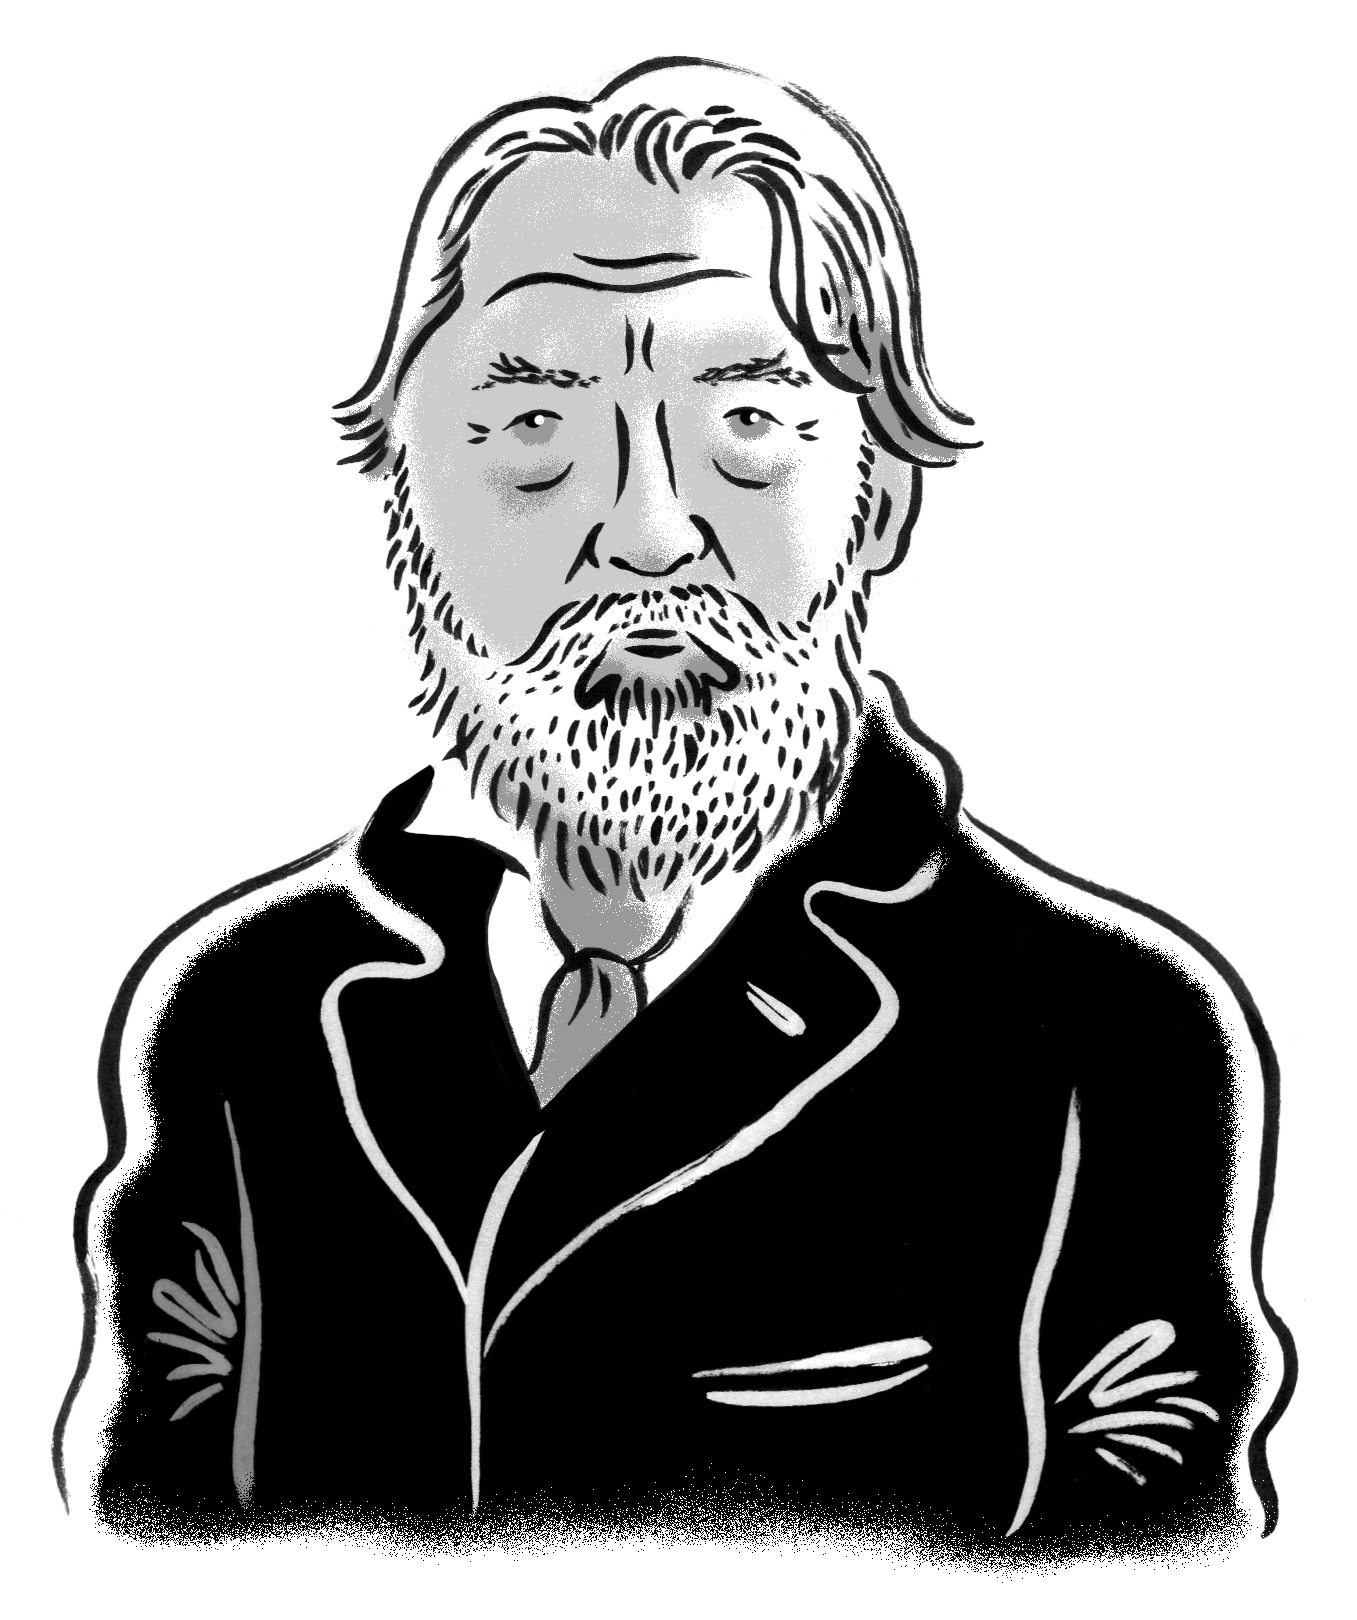
\includegraphics[width=6cm]{./imgs/autor3.jpg}
\end{center}

\chapter{Мuмu}


Em uma rua afastada de Moscou, em uma casa cinzenta de colunas brancas,
com uma mansarda e um terraço retorcido, morava outrora uma fidalga, uma
viúva rodeada de numerosos criados. Seus filhos serviam em São
Petersburgo, as filhas tinham se casado; ela saía pouco e passava
sozinha os últimos anos de sua velhice avara e tediosa. A luz do seu
dia, infeliz e sombrio, se apagara havia tempos e seu entardecer era
mais negro do que a noite.

De todos os seus serviçais, o mais notável era o caseiro Guerássim, um
homem de quase dois metros de altura, com compleição de
\emph{bogatyr}\footnote{\emph{Bogatyr,} guerreiro mitológico de
  narrativas russas antigas.} e surdo"-mudo de nascença. A patroa
trouxe"-o de uma aldeia, onde ele morava sozinho, numa pequena
isbá,\footnote{Isbá, casa de camponês na Rússia, tradicionalmente
  feita de troncos.} separado dos irmãos, e considerava"-o talvez o mais
correto dos mujiques\footnote{Mujique, campônio russo, assim designado
  principalmente antes de 1917.} no pagamento dos tributos senhoriais.
Dotado de força extraordinária, trabalhava por quatro --- as tarefas
fluíam em suas mãos, e era divertido vê"-lo quando lavrava e, apoiando
com força as mãos enormes no arado de madeira, parecia abrir o peito
rijo da terra sozinho, sem ajuda de cavalos, ou quando, no dia de São
Pedro, manejava a gadanha de forma tão arrasadora, que poderia arrancar
pela raiz um bosque inteiro de bétulas\footnote{Bétula (berioza), árvore
  com o caule de casca branco"-prateada que é um símbolo nacional na
  Rússia.} jovens, ou quando debulhava sem cessar com um mangual de mais
de dois metros,\footnote{No original, foi usado \emph{archin,} antiga
  medida russa equivalente a 71,1 cm. Todas as ocorrências do termo
  foram adaptadas.} subindo e descendo, como uma alavanca, os músculos
firmes e alongados de seu ombro. O silêncio constante conferia uma
importância solene a seu trabalho inesgotável. Era um mujique esplêndido
e, se não fosse por seu infortúnio, qualquer moça se casaria com ele de
bom grado\ldots{} Eis que levaram Guerássim a Moscou, compraram"-lhe botas,
fizeram"-lhe um cafetã para o verão e um sobretudo de peles para o
inverno, colocaram"-lhe uma vassoura e uma pá na mão, e tornaram"-no
caseiro.

No começo, ele não gostara da nova vida de jeito nenhum. Desde criança,
estava acostumado ao trabalho no campo, ao modo de vida da aldeia.
Privado, devido ao seu infortúnio, da companhia de pessoas, crescera
mudo e poderoso, como uma árvore em solo fecundo\ldots{} Transferido para a
cidade, não entendia o que lhe acontecia --- aborrecia"-se e ficava
perplexo como um touro jovem e saudável recém"-tirado de um pasto onde a
grama suculenta roçava"-lhe a barriga. Pegaram Guerássim, colocaram"-no em
um vagão de trem, e pronto; envolvendo o corpo obeso dele ora com fumaça
e fagulhas, ora com vapor ondulante, arrastavam"-no, arrastavam"-no com
batidas e ganidos, mas para onde o arrastavam só Deus sabia! Depois da
dureza dos trabalhos no campo, as tarefas de Guerássim em sua nova
função pareciam"-lhe brincadeiras; em meia hora, tudo já estava pronto e
ele ora voltava a ficar parado no meio do pátio, olhando boquiaberto
para todos os transeuntes, como se quisesse obter deles a solução do
enigma de sua situação, ora ia repentinamente para algum canto e,
jogando para longe a vassoura e a pá, atirava"-se de cara ao chão,
deitando"-se de bruços por horas a fio, imóvel, como uma fera capturada.
Mas a pessoa se acostuma a tudo, e Guerássim acostumou"-se, finalmente,
ao modo de vida urbano. Suas obrigações não eram muitas; consistiam em
manter o pátio limpo, carregar uma pipa de água duas vezes por dia,
rachar e trazer lenha para a cozinha e para casa, não admitir estranhos
e fazer a vigia noturna. E deve"-se dizer que tudo era cumprido com zelo;
em seu pátio, jamais havia um cachorro à toa, nem lixo; se, quando
estava lamacento, o rocim alquebrado que fora colocado sob seu comando
ficasse atolado com a telega carregada de água, bastava a Guerássim
mover o ombro para tirar do lugar não apenas a carroça, como o próprio
cavalo; quando se punha a rachar lenha, seu machado retinia como vidro,
com estilhaços e achas voando por todas as direções, e, no que se
referia a pessoas de fora, depois que, uma noite, capturando dois
ladrões, ele batera a testa de um contra a do outro de tal jeito que nem
fora preciso levá"-los à polícia, todos dos arredores começaram a
respeitá"-lo muito; mesmo quem passava por lá de dia e não era vigarista,
apenas gente desconhecida, ao ver o terrível caseiro, acenava e gritava
cumprimentos, como se ele pudesse ouvir esses gritos. Com o resto dos
criados, Guerássim encontrava"-se em relações não exatamente amigáveis
--- eles o temiam ---, mas respeitosas; considerava"-os sua gente. Ele
compreendia os sinais que usavam para comunicar"-se com ele, cumprindo
com exatidão todas as ordens, mas também conhecia seus direitos, de modo
que ninguém ousava sentar"-se em seu lugar à mesa. Em geral, Guerássim
era de temperamento rigoroso e sério, gostava de ordem em tudo; mesmo os
galos, em sua presença, não se atreviam a brigar --- ai deles! Se os
flagrasse, pegava"-os pelas pernas, girava"-os dez vezes no ar, como uma
roda, e arremessava"-os para lados opostos. No pátio da patroa também
havia gansos, mas o ganso, como se sabe, é ave importante e sensata;
Guerássim os respeitava, cuidava deles e os alimentava; ele mesmo
parecia um ganso da estepe. Designaram"-lhe um cubículo em cima da
cozinha; ele se arrumou por lá sozinho, segundo seu gosto, armou uma
cama de tábuas de carvalho sobre quatro cepos --- um verdadeiro leito de
\emph{bogatyr;} podiam colocar mais de uma tonelada\footnote{No
  original, foi usado \emph{pud}, antiga medida de peso equivalente a
  16,3 kg. Todas as ocorrências do termo foram adaptadas.} em cima dela
que não cederia ---; embaixo da cama, havia um baú resistente; no canto,
uma mesinha igualmente robusta e, junto à mesinha, uma cadeira baixa de
três pés tão sólida, que acontecia de o próprio Guerássim erguê"-la para
vê"-la cair, achando graça nisso. O cubículo era fechado com um cadeado
que lembrava um \emph{kalatch},\footnote{\emph{Kalatch}, pão de trigo
  em forma de cadeado.} só que preto; o caseiro nunca tirava da
cintura a chave do cadeado. Não gostava que fossem até lá.

Assim passou um ano, no fim do qual ocorreu a Guerássim um pequeno
incidente.

A velha fidalga da qual ele era caseiro seguia os antigos costumes em
tudo, mantendo uma criadagem numerosa; em sua casa havia não apenas
lavadeiras, costureiras, marceneiros, alfaiates e modistas, mas até um
seleiro, que também era veterinário e médico da criadagem; havia um
médico da casa para a patroa e, por fim, um sapateiro de nome Kapiton
Klímov, um beberrão amargurado. Klímov considerava"-se uma criatura
ultrajada e não valorizada à altura de seus méritos, um homem criado na
capital, instruído, que não devia viver em Moscou,\footnote{Naquela
  época, a capital da Rússia era São Petersburgo.} sem ocupação, em um
fim de mundo, e, se bebia, como ele mesmo dizia pausadamente e batendo
no peito, bebia exatamente de pesar. Eis que, uma vez, surgiu uma
conversa a seu respeito entre a patroa e seu primeiro mordomo, Gavrila,
um homem que, a julgar apenas por seus olhinhos amarelados e nariz de
pato, parecia ter sido destinado à chefia. A patroa lamentava a
moralidade corrompida de Kapiton, que na véspera fora encontrado caído
no meio da rua.

--- E então, Gavrila? --- disse ela, de repente. --- Não devíamos
casá"-lo? O que acha? Pode ser que crie juízo.

--- Por que não casá"-lo, senhora? É possível, senhora --- respondeu
Gavrila ---, até seria muito conveniente, senhora.

--- Sim, mas quem casaria com ele?

--- Claro, senhora. Aliás, será como a senhora quiser. Afinal, ele, por
assim dizer, pode satisfazer alguém; não é de se jogar fora.

--- Será que Tatiana gosta dele?

Gavrila quis retrucar algo, mas mordeu os lábios.

--- Sim!\ldots{} Que case com Tatiana --- decidiu a patroa, cheirando rapé
com satisfação. --- Ouviu?

--- Sim, senhora --- proferiu Gavrila e saiu.

De volta ao seu quarto (ficava em um anexo, quase todo atravancado de
baús reforçados com chapas de ferro), Gavrila primeiro despachou sua
mulher e depois se sentou junto à janela para refletir. A ordem
inesperada da patroa, pelo visto, o havia desconcertado. Por fim,
levantou"-se e mandou chamar Kapiton Klímov. Kapiton apareceu\ldots{} Mas,
antes de informar ao leitor a conversa que se desenrolou entre os dois,
julgamos proveitoso contar, em poucas palavras, quem era a Tatiana que
queriam casar com Kapiton e por que a conduta da patroa havia deixado o
mordomo embaraçado.

Tatiana, que desempenhava, como referido acima, a função de lavadeira
(aliás, como lavadeira hábil e treinada, era encarregada apenas da roupa
de baixo fina), era uma mulher de vinte e oito anos, pequena, magra,
loira, com marcas de nascença na face esquerda. Marcas de nascença na
face esquerda são consideradas mau sinal na Rússia --- presságios de uma
vida infeliz\ldots{} Tatiana não podia se gabar de sua sorte. Desde muito
nova, fora mantida em linha dura; trabalhava por duas, nunca teve
mostras de afeto; recebia as piores roupas e a menor remuneração; seus
parentes e nada eram a mesma coisa: um tio velho despenseiro, largado na
aldeia por inépcia, e uns tios mujiques, e nada mais. Numa época, ela
passara por beldade, mas a beleza logo a abandonou. Seu temperamento era
muito pacífico, ou melhor, assustado; para consigo mesma sentia absoluta
indiferença, temendo os outros mortalmente; pensava apenas em como
terminar as tarefas no prazo, nunca falava com ninguém e estremecia só à
menção do nome da patroa, embora esta mal colocasse os olhos nela.
Quando Guerássim foi trazido da aldeia, a lavadeira quase morreu de
susto à vista daquela figura imensa, tentava de todas as formas
evitá"-lo, chegava a semicerrar os olhos quando lhe ocorria passar ao
lado dele, correndo dе casa para a lavanderia. No começo Guerássim não
lhe dava atenção, depois começou a achar graça quando se deparava com
ela, depois passou a reparar nela e, finalmente, não lhe tirava os
olhos. Ela caiu no seu agrado; fosse pela expressão dócil, fosse pela
timidez dos movimentos, só Deus sabia! Eis que, um dia, ela entrava no
pátio, erguendo cuidadosamente nos dedos abertos uma blusa engomada da
patroa, quando alguém a pegou com força pelo cotovelo; ela se virou e
gritou: atrás dela, postava"-se Guerássim. Com um sorriso estúpido e
murmurando carinhosamente, estendia"-lhe um bolo de mel em forma de galo,
com ouropel na cauda e nas asas. Ela quis recusar, porém ele enfiou o
doce em sua mão, meneou a cabeça e partiu, virando"-se e murmurando
amigavelmente. Desde então, não lhe deu sossego: não importava onde
Tatiana fosse, lá estava ele indo ao seu encontro, sorria, murmurava,
abanava os braços, tirava subitamente uma fita do peito e dava a ela com
ímpeto, com a vassoura limpava o pó na frente dela. A pobre moça
simplesmente não sabia como se portar e o que fazer. Logo a casa inteira
ficou sabendo das artes do caseiro mudo; zombarias, gracejos, palavras
maliciosas choveram sobre Tatiana. De Guerássim, contudo, poucos
quiseram escarnecer: ele não gostava de piadas e, em sua presença, a
lavadeira também era deixada em paz. Quisesse ou não, a moça estava sob
sua proteção. Como todo surdo"-mudo, ele era muito perspicaz e entendia
muito bem quando estavam rindo dele ou dela. Uma vez, no almoço, a
roupeira, chefe de Tatiana, começou a, como dizem, amolá"-la, a ponto de
a coitada não saber onde enfiar os olhos e por pouco não chorar de
desgosto. Guerássim ergueu"-se de repente, estendeu a mão imensa,
colocou"-a na cabeça da roupeira e fitou"-a com um furor tão sombrio, que
a mulher se curvou sobre a mesa. Todos se calaram. Guerássim voltou a
pegar a colher e continuou sorvendo sua sopa de repolho. ``Arre, diabo
surdo, \emph{léchi}!'',\footnote{\emph{Léchi,} ser da mitologia eslava
  que habita as florestas e protege os animais e muitas vezes tem a
  forma de um homem gigante e abrutalhado.} disseram todos a meia voz,
enquanto a roupeira levantava"-se e ia para o quarto das criadas. E,
outra vez, reparando que Kapiton, aquele mesmo de quem acabamos de
falar, tratava Tatiana com amabilidade excessiva, Guerássim chamou"-o com
o dedo, levou"-o ao galpão das carroças e, pegando pela extremidade um
tirante, ameaçou"-o com ele, de forma ligeira, mas significativa. Desde
então, ninguém falou mais com Tatiana. E por tudo isso Guerássim não
sofreu consequências. Na realidade, a roupeira, que desfaleceu ao entrar
correndo no quarto das criadas, agiu de forma tão hábil, que, no mesmo
dia, a notícia do comportamento rude de Guerássim chegou à patroa. A
velha extravagante apenas riu e, para grande ultraje da roupeira,
fez"-lhe repetir algumas vezes como o caseiro tinha esticado a mão até
ela e, no dia seguinte, mandou um rublo a ele. A fidalga o respeitava
como guardião fiel e forte. Guerássim a temia bastante, mesmo assim
contava com sua benevolência e estava prestes a pedir"-lhe permissão para
se casar com Tatiana. Esperava apenas o cafetã novo que o mordomo lhe
prometera, para comparecer diante da patroa com aspecto decente, quando,
de repente, passou pela cabeça dessa mesma patroa a ideia de casar
Tatiana com Kapiton.

O leitor agora compreende com facilidade o motivo do embaraço que se
apoderou do mordomo Gavrila após a conversa com a senhora. ``É claro'',
pensou ele, sentado junto à janela, ``que a senhora respeita Guerássim
(o mordomo sabia disso muito bem, por isso também o favorecia), mesmo
assim é uma criatura privada de palavras; não tenho como informar à
senhora que ele está cortejando a Tatiana. E, vamos e venhamos, que tipo
de marido ele daria? Mas, por outro lado, Deus me livre, quando ficar
sabendo que Tatiana irá se casar com Kapiton, o \emph{léchi} quebrará
tudo em casa, ai"-ai. Afinal, não dá para confrontá"-lo; com o perdão da
palavra, um diabo desses, não há jeito de convencê"-lo\ldots{} É a pura
verdade!\ldots{}''

A aparição de Kapiton interrompeu a linha de raciocínio de Gavrila. O
sapateiro leviano entrou, colocou as mãos para trás, encostou"-se com
desembaraço no canto da parede junto à porta, pondo o pé direito na
frente do esquerdo, e sacudiu a cabeça. ``Estou aqui. O que deseja?''

Gavrila olhou para Kapiton e tamborilou no umbral da janela. Kapiton
apenas apertou um pouco os olhos inexpressivos, mas não os baixou,
chegou a esboçar um sorriso e passou a mão nos cabelos embranquecidos
que se eriçavam para todas as direções, como se dissesse: ``Pois bem,
estou aqui. O que está olhando?''.

--- É bonito --- disse Gavrila e se calou. --- É bonito, não há o que
dizer!

Kapiton apenas contraiu os ombros. ``Mas você por acaso é melhor?'',
pensou consigo mesmo.

--- Bem, olhe para si mesmo, olhe --- prosseguiu Gavrila com censura
---, com quem você se parece?

Kapiton lançou um olhar tranquilo para a própria sobrecasaca surrada e
em farrapos, as calças remendadas, examinou com particular atenção as
botas esburacadas, especialmente aquela em cujo bico apoiava com
afetação seu pé direito, então voltou a encarar o mordomo.

--- E então, senhor?

--- E então, senhor? --- respondeu Gavrila. --- E então, senhor? Você
ainda diz ``e então''? Parece um diabo, com o perdão da palavra, mas é
isso que parece.

Kapiton piscou os olhinhos rapidamente.

``Xingue, xingue, Gavrila Andréitch'', voltou a pensar consigo mesmo.

--- Afinal, você ficou bêbado de novo --- começou Gavrila. --- Não foi?
Hem? Ora, responda.

--- Por fraqueza de saúde, sujeitei"-me de fato ao uso de bebidas
alcoólicas --- replicou Kapiton.

--- Por fraqueza de saúde!\ldots{} Você recebe pouca punição, é isso; quando
vivia em Píter,\footnote{Píter, apelido da cidade de São Petersburgo.}
era aprendiz\ldots{} Aprendeu muito! Só fica comendo pão de graça.

--- Nesse caso, Gavrila Andréitch, tenho apenas um juiz: o senhor Deus,
e mais ninguém. Só ele sabe que homem sou neste mundo e se como pão de
graça. No que se refere às considerações sobre bebedeira, nesse caso, o
culpado não sou eu, mas um camarada; ele me atraiu, mas escafedeu"-se
espertamente, ou seja, foi embora, enquanto eu\ldots{}

--- Enquanto você ficou na rua, energúmeno. Ah, que homem leviano! Pois
bem, a questão não é essa --- continuou o mordomo. --- É o seguinte. A
patroa\ldots{} --- ele fez uma pausa. --- A patroa deseja que você se case.
Ouviu? Ela acha que você vai criar juízo ao se casar. Entendeu?

--- Como não entender, senhor.

--- Pois bem. Na minha opinião, seria melhor enquadrá"-lo. Enfim, a
questão não é essa. E então? Você concorda?

Kapiton sorriu, mostrando os dentes.

--- O matrimônio é uma coisa boa para o homem, Gavrila Andréitch; eu, de
minha parte, terei muita satisfação.

--- Pois bem --- replicou Gavrila, pensando consigo mesmo: ``Não há o
que dizer, o homem fala bem''. --- Só tem uma coisa --- prosseguiu em
voz alta ---, a noiva que encontraram é boa demais para você.

--- Quem é, se permite a curiosidade?\ldots{}

--- Tatiana.

--- Tatiana?

E Kapitоn esfregou os olhos e se afastou da parede.

--- Ora, por que essa agitação?\ldots{} Por acaso ela não é do seu agrado?

\textls[-26]{--- Como não seria, Gavrila Andréitch! Nada contra ela, é trabalhadora,
uma moça pacífica\ldots{} Mas o senhor sabe, Gavrila Andréitch, que o
\emph{léchi}, aquela \emph{kikímora}\footnote{\emph{Kikímora,}
  criatura normalmente feminina da mitologia eslava, um espírito nocivo
  do lar que pode ser contraposto ao \emph{domovoi,} o qual protege as
  casas.} da estepe, vive atrás dela\ldots{}}

--- Sei, meu caro, sei de tudo --- interrompeu"-o o mordomo com desgosto
---, mas veja\ldots{}

--- Tenha piedade, Gavrila Andréitch! Ele vai me matar, por Deus, vai me
matar como uma mosca, com uma palmada; veja a mão dele, tenha a bondade
de examinar que mão ele tem; é simplesmente a mão de Mínin e
Pojárski.\footnote{Kuzmá Mínin (segunda metade séc. \textsc{xvi}--1616) e
  Dmítri Pojárski (1577--1642), heróis da luta russa contra os
  poloneses, no século \textsc{xvii}.} Pois ele é surdo, bate e não escuta, e
como bate! Agita os punhos sem perceber. E não há nenhuma possibilidade
de acalmá"-lo. E sabe por que, Gavrila Andréitch? Porque ele é surdo como
uma porta e, ainda por cima, estúpido. É uma espécie de fera, uma besta,
Gavrila Andréitch, ou pior do que uma besta, um brutamontes\ldots{} Por que
devo agora sofrer na mão dele? Claro que eu não valho nada agora: sou um
homem conformado, gasto, sebento como um pote da velha Kolomna, só que
mesmo assim sou um homem, e não um traste qualquer.

--- Sei, sei, não precisa se descrever\ldots{}

--- Senhor Deus! --- prosseguiu o sapateiro com ardor. --- Quando será o
fim? Quando, senhor? Sou um pobre"-diabo, um pobre"-diabo sem saída! Que
destino, que destino o meu, pense bem! Nos anos de juventude apanhei do
patrão alemão, na flor da idade do próprio irmão e, por fim, na idade
madura, veja a que ponto cheguei\ldots{}

--- Ah, que alma frouxa --- afirmou Gavrila. --- Para que exagerar desse
jeito? Que coisa!

--- Como não, Gavrila Andréitch? Não tenho medo da surra, Gavrila
Andréitch. Que o Senhor me castigue entre quatro paredes, mas me saúde
diante das pessoas, e continuarei a ser um homem entre os outros, mas
aqui de quem serei obrigado a apanhar\ldots{}

--- Pois bem, vá embora --- interrompeu"-o Gavrila, impaciente.

Kapiton virou"-se e saiu lentamente.

--- Mas suponhamos que ele não existisse --- gritou o mordomo na direção
dele ---, você concordaria?

--- Ao seu dispor --- retrucou Kapiton e desapareceu.

A eloquência não o abandonava mesmo em ocasiões extremas.

O mordomo deu algumas voltas pelo quarto.

--- Pois bem, agora chame Tatiana --- disse finalmente.

Em alguns instantes, Tatiana veio, quase inaudível, e parou na soleira.

--- O que deseja, Gavrila Andréitch? --- ela disse em voz baixa.

O mordomo olhou"-a fixamente.

--- Pois bem --- proferiu ele ---, Taniucha,\footnote{Taniucha,
  diminutivo de Tânia, apelido Tatiana.} quer se casar? A patroa arrumou um noivo para
você.

--- Continue, Gavrila Andréitch. E quem foi designado como meu noivo?
--- acrescentou ela, indecisa.

--- Kapiton, o sapateiro.

--- Continue, senhor.

--- É um homem leviano, isso é certo. Mas a patroa tem esperança em você
nesse caso.

--- Sim, senhor.

--- O único problema\ldots{} é esse surdo, Guerássim, ele a corteja. Como
você enfeitiçou esse urso? Pois ele é capaz de matá"-la, um urso
desses\ldots{}

--- Vai matar, Gavrila Andréitch, vai matar sem falta.

--- Vai matar\ldots{} Ora, isso nós veremos. Como você diz que vai matar? Por
acaso ele tem direito de matá"-la? Julgue você mesma.

--- Não sei se tem direito ou não, Gavrila Andréitch.

--- Cada uma! Você não lhe prometeu nada\ldots{}

--- O que o senhor deseja?

O mordomo calou"-se e pensou um pouco: ``Que alma submissa!''.

--- Pois bem --- acrescentou ---, ainda falarei com você, agora vá,
Taniucha; estou vendo que você é realmente humilde.

Tatiana virou"-se, apoiando"-se de leve no batente, e saiu.

``Mas pode ser que amanhã a patroa se esqueça dessas núpcias'', pensou o
mordomo. ``E para que eu me agitei à toa? Vamos amarrar esse desordeiro;
se for o caso, chamaremos a polícia\ldots{}''

--- Ustínia Fiódorovna! --- gritou bem alto à esposa. --- Sirva o
samovar,\footnote{Samovar, utensílio tradicional russo usado para
  ferver a água do chá.} minha cara\ldots{}

Tatiana passou quase o dia inteiro na lavanderia. Chorou um pouco,
enxugou as lágrimas, então voltou ao trabalho de antes. Kapiton ficou
até tarde da noite em uma taberna com um conhecido de ar sombrio, a quem
contou em detalhes como morava, em Píter, com um fidalgo que era bom em
tudo, observador da ordem, embora se permitisse umа pequenа fraqueza:
tomava muitas bebedeiras e, quanto ao sexo feminino, simplesmente
aceitava qualquer tipo\ldots{} O camarada sombrio só fazia coro com ele; mas,
quando Kapiton finalmente anunciou que, no dia seguinte, por uma
contingência, seria obrigado a se matar, o camarada observou que estava
na hora de dormir. E eles se separaram com rudeza e em silêncio.

Enquanto isso, as expectativas do mordomo não se cumpriram. A patroa
estava tão tomada pela ideia do casamento de Kapiton, que, mesmo de
noite, falou disso sem parar com uma de suas acompanhantes, que era
mantida em casa unicamente para o caso de insônia e, como um cocheiro
noturno, dormia de dia. Quando Gavrila foi fazer o relatório à fidalga,
depois do chá, a primeira pergunta dela foi: e o nosso casamento, está
andando? Naturalmente ele respondeu que não podia andar melhor e que
Kapiton, nesse mesmo dia, viria lhe apresentar seus respeitos. A patroa
estava algo indisposta; ocupou"-se dos negócios por pouco tempo. O
mordomo retornou a seu quarto e convocou um conselho. O assunto
certamente requeria um julgamento especial. Claro que Tatiana não o
contrariou; mas Kapiton afirmou em alto e bom som que tinha apenas uma
cabeça, não duas nem três\ldots{} Guerássim lançava olhares severos e rápidos
a todos, não se afastava da ala das moças e parecia adivinhar que
tramavam algo de ruim contra ele. Os reunidos (entre os quais estava um
velho copeiro, apelidado Tio Cauda, a quem todos se dirigiam
respeitosamente atrás de conselhos, embora só ouvissem dele: ah, que
coisa; sim, sim, sim) começaram, por segurança, para qualquer
eventualidade, trancando Kapiton no quartinho da máquina de decantar
água e puseram"-se a pensar com seriedade. Claro que seria fácil recorrer
à força; mas Deus nos livre! Haveria gritaria, a patroa seria
importunada, uma desgraça! O que fazer? Pensaram, pensaram e, por fim,
inventaram algo. Observaram repetidamente que Guerássim não podia
suportar beberrões\ldots{} Sentado ao portão, virava"-se indignado toda vez
que passava um sujeito alcoolizado, com passos vacilantes e a pala do
quepe caída na orelha. Resolveram instruir Tatiana a fingir"-se bêbada e
a passar por Guerássim cambaleando e tropicando. A pobre moça discordou
durante muito tempo, mas convenceram"-na; de mais a mais, ela mesma
percebia que, de outra forma, não afastaria seu adorador. E se foi.
Deixaram Kapiton sair do quartinho: em todo caso, o assunto lhe dizia
respeito. Guerássim estava sentado em um postezinho, junto ao portão, e
cavoucava a terra com uma pá\ldots{} De todos os cantos, por trás de todas as
cortinas das janelas olhavam para ele\ldots{}

A artimanha não podia ter tido mais êxito. Ao ver Tatiana, ele no
começo, como de hábito, meneou a cabeça com um murmúrio carinhoso;
depois fitou a lavadeira atentamente, deixou cair a pá, levantou"-se num
pulo, aproximou"-se, e levou seu rosto para perto do dela\ldots{} De pavor,
ela cambaleou ainda mais e fechou os olhos\ldots{} Ele a tomou pelo braço,
correu pelo pátio e, entrando com ela no aposento em que o conselho
estava reunido, empurrou"-a para Kapiton. Tatiana ficou petrificada\ldots{}
Guerássim, ali postado, olhou para ela, fez um aceno com a mão, riu e
foi para seu cubículo, pisando forte\ldots{} Ficou horas inteiras sem sair de
lá. O boleeiro Antipka depois contou que, através de uma fresta, via
como Guerássim, sentado na cama, com a mão na face, volta e meia cantava
com murmúrios, em tom baixo, compassado, ou seja, balançava"-se de olhos
fechados e sacudia a cabeça, como um cocheiro ou um puxador de sirgas ao
entoar canções tristes. Antipka sentira um arrepio e se afastara da
fresta. Quando, no dia seguinte, Guerássim saiu do cubículo, não era
possível notar nele nenhuma mudança em particular. Apenas parecia mais
sombrio e não dava a menor atenção nem para Tatiana nem para Kapiton.
Nessa mesma noite, os dois dirigiram"-se à patroa com gansos debaixo do
braço e, em uma semana, casaram"-se. No dia das bodas, Guerássim não
alterou seu comportamento em nada; apenas voltou do rio sem água: de
algum jeito, quebrou a pipa no meio do caminho e, à noite, na
estrebaria, limpou e esfregou seu cavalo com tamanho empenho que este
cambaleou, como um talo ao vento, bambeando ao passar de uma perna para
outra sob os punhos de ferro do caseiro.

Tudo isso aconteceu na primavera. Passou um ano, no decorrer do qual
Kapiton embebedou"-se de vez e, como um completo imprestável, foi mandado
com a mulher, em um comboio de carroças, para uma aldeia distante. No
dia da partida, ele inicialmente se fez de valente, assegurando que,
fosse para onde fosse, mesmo para onde Judas perdeu as botas, aguentaria
firme; mas, depois, deprimiu"-se, começou a se queixar de que seria
levado para um lugar de gente sem educação e, por fim, ficou tão fraco,
que não conseguia nem colocar o próprio chapéu; uma alma compassiva
botou"-o em sua testa, endireitou a aba e ergueu"-a com uma palmada.
Quando tudo estava pronto e os mujiques já estavam com as mãos nas
rédeas, esperando apenas as palavras ``vão com Deus'', Guerássim saiu de
seu cubículo, aproximou"-se de Tatiana e deu"-lhe, como lembrança, um
lenço vermelho de algodão que comprara um ano antes para ela. Tatiana,
que até esse instante suportara com grande indiferença todas as
vicissitudes de sua vida, não aguentou, debulhou"-se em lágrimas е,
sentando"-se na telega, deu três beijos cristãos em Guerássim. Ele quis
acompanhá"-la até a barreira e partiu ao lado de sua telega, mas de
repente parou no vau da Crimeia,\footnote{Saindo do rio Moscou, não
  longe do Krêmlin, fica o vau da Crimeia (\emph{Krýmski brod}). Sobre
  ele fizeram uma ponte e, na época de Turguêniev, às vezes, mencionando
  o vau, se referiam a ela.} fez um aceno com a mão e marchou ao longo
do rio.

Tudo ocorreu ao entardecer. Ele caminhava em silêncio com os olhos fitos
na água. De súbito, teve a impressão de que algo se revolvia no lodo,
junto à margem. Inclinou"-se e avistou um cachorro pequeno, branco de
manchas pretas que, apesar de todo o seu esforço, não conseguia sair da
água, debatia"-se, escorregava e tremia inteiro com seu corpo molhado e
úmido. Guerássim olhou para o cãozinho infeliz, pegou"-o com uma mão,
enfiou"-o no peito e dirigiu"-se para casa a passos largos. Entrou em seu
cubículo, acomodou o filhote salvo na cama e cobriu"-o com seu sobretudo
pesado, então correu primeiro à estrebaria atrás de palha, depois à
cozinha atrás de uma xícara de leite. Levantando o casaco e estendendo a
palha com cuidado, colocou o leite na cama. O pobre cachorrinho não
tinha mais de três semanas; fazia pouco tempo que seus olhos se abriram,
um olho até parecia um pouco maior do que o outro; ainda não sabia beber
da xícara e só tremia e apertava a vista. Guerássim pegou o filhote com
delicadeza, colocando dois dedos na nuca dele, e baixou seu focinho até
o leite. O cachorro de repente começou a beber com avidez, fungando,
sacudindo"-se, engasgando. Guerássim olhou, olhou, até que repentinamente
sorriu\ldots{} Cuidou dele a noite inteira, embalou"-o, limpou"-o e, por fim,
ao seu lado teve um sono alegre e tranquilo.

Nenhuma mãe cuida tanto de seu bebê quanto Guerássim cuidou de sua
pupila (o cachorro revelou"-se uma cadela). No começo, ela era muito
fraca, mirrada e feia, mas aos poucos melhorou e se aprumou e, uns oito
meses depois, graças à incansável dedicação de seu salvador,
transformou"-se em uma \emph{spaniel} muito jeitosa, de orelhas
compridas, cauda felpuda em forma de tubo e olhos grandes e expressivos.
Apegou"-se apaixonadamente a Guerássim e não se afastava um passo dele,
sempre balançando o rabo. Ele até lhe deu um apelido --- os mudos sabem
que seus murmúrios despertam atenção e chamou"-a de Mumu. Todos da casa
gostaram dela e também passaram a chamá"-la de Mumu. Ela era
extraordinariamente inteligente, fazia festa para todo mundo, mas só a
Guerássim amava. E ele próprio a amava perdidamente\ldots{} Não gostava
quando outros a acariciavam: se temia por ela ou se tinha ciúme, só Deus
sabia! Mumu o acordava pela manhã, puxando"-o pela manga; trazia"-lhe
pelas rédeas o velho cavalo que transportava a água, com quem vivia em
grande amizade; com aspecto imponente ela ia com o dono até o rio,
vigiava suas vassouras e pás, não deixava ninguém entrar em seu
cubículo. O caseiro fez uma abertura na porta especialmente para ela,
que como que sentia que apenas no cubículo de Guerássim era a verdadeira
dona da casa e, assim que lá entrava, com ar satisfeito saltava na cama.
De madrugada, a cachorra não dormia de jeito nenhum, mas não latia
indistintamente, como um vira"-lata estúpido que, sentado nas patas
traseiras, erguendo a fuça e semicerrando os olhos, late simplesmente de
tédio para as estrelas, normalmente três vezes seguidas. Não! A vozinha
fina de Mumu nunca soava à toa: ou um estranho passava perto da cerca,
ou um ruído ou um sussurro suspeito se erguia em algum lugar\ldots{} Em suma,
ela vigiava muito bem. Além dela, havia no pátio um velho cão amarelo de
manchas pardas chamado Lobinho, que nunca era solto, nem de madrugada, e
ele mesmo, devido à sua decrepitude, jamais reclamava por sua liberdade
--- ficava deitado, enrodilhado em sua casinha, e só de vez em quando
emitia um latido roufenho, quase inaudível, que interrompia de imediato,
como se sentisse quão inútil era. Na casa senhorial, Mumu não entrava e,
quando Guerássim levava lenha para os aposentos, ela sempre ficava para
trás, aguardando"-o, impaciente, nos degraus da entrada, de orelha em pé
e virando a cabeça, ora para a direita, ora subitamente para a esquerda,
ao menor barulho que ouvia atrás das portas\ldots{}

\begin{figure}%[ht!]
\vspace*{-1.8cm}
\hspace*{-1.8cm}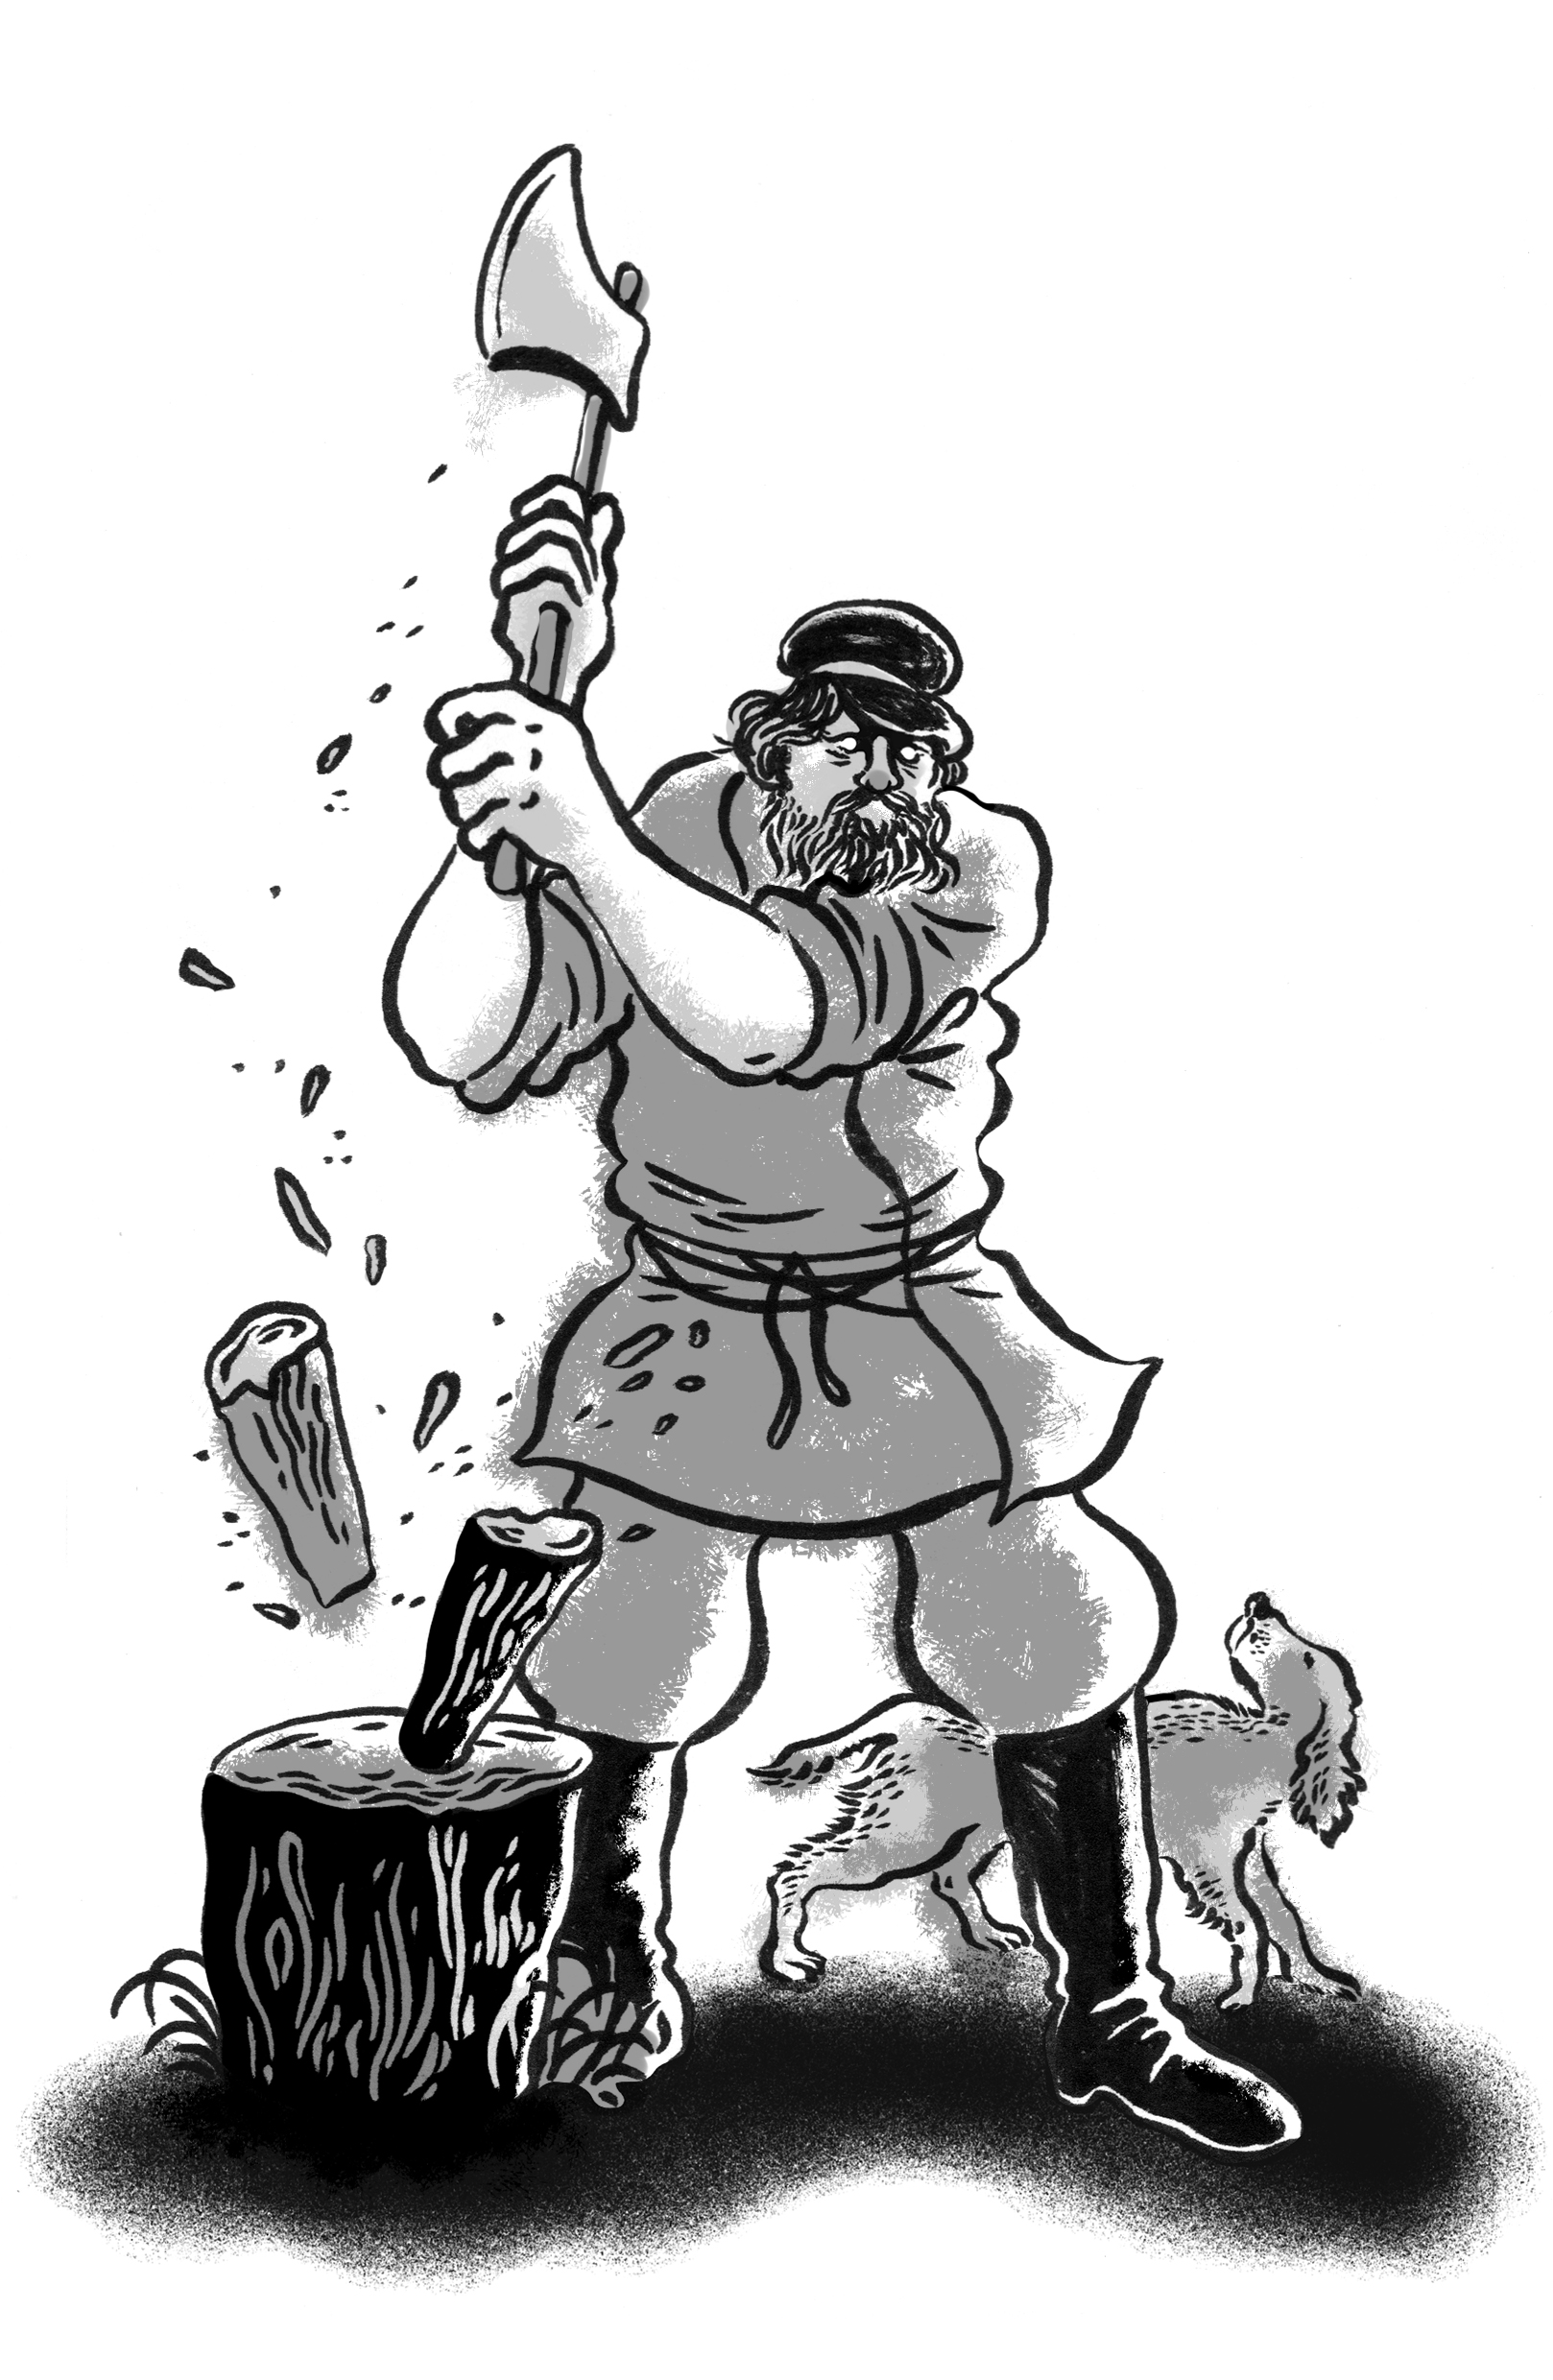
\includegraphics{./imgs/cena3.jpg}
\end{figure}

Assim passou mais um ano. Guerássim continuou com seus afazeres de
caseiro e estava muito satisfeito com seu destino quando, de repente,
ocorreu uma circunstância inesperada\ldots{}

Foi o seguinte: em um lindo dia de verão, a patroa perambulava pela sala
de visitas com suas comensais. Estava bem"-disposta, ria e gracejava; as
comensais também riam e gracejavam, mas não se sentiam particularmente
contentes: nessa casa, não gostavam muito quando a patroa se encontrava
nesse estado, porque, em primeiro lugar, ela sempre exigia de todos uma
participação imediata e plena e se zangava se o rosto de alguém não
expressava satisfação; em segundo lugar, esses arroubos duravam pouco
tempo e normalmente se transformavam em um humor sombrio e azedo. Nesse
dia, ela acordara alegre: nas cartas, saíram"-lhe quatro valetes --- a
realização dos desejos (sempre tirava a sorte pela manhã) --- e o chá
lhe pareceu especialmente saboroso, motivo pelo qual a copeira recebeu
elogios em palavras e dez copeques em dinheiro. Com um sorriso doce nos
lábios enrugados, a patroa, passeando pela sala, se aproximou da janela.
Em frente, tinham feito um jardinzinho e, no canteiro do meio, embaixo
de um arbusto de rosas, Mumu estava deitada roendo um osso, meticulosa.
A patroa a viu.

--- Meu Deus! --- ela gritou de repente. --- Que cachorro é esse?

A comensal a quem a patroa havia se dirigido hesitou, pobrezinha, com a
preocupação angustiada que normalmente se apossa dos dependentes quando
ainda não sabem ao certo como entender a exclamação da autoridade.

--- N\ldots{} n\ldots{} não sei, senhora --- balbuciou ---, parece que é do mudo.

--- Meu Deus! --- interrompeu a patroa. --- Mas é um cachorro muito
engraçadinho! Mande trazê"-lo para mim. Faz tempo que ele o tem? Como é
que eu não o vi até agora?\ldots{} Mande trazê"-lo.

A comensal imediatamente voou para a antessala.

--- Homem, homem! --- gritou. --- Traga logo Mumu! Está no jardinzinho.

--- E se chama Mumu --- proferiu a patroa ---, um nome muito bonito.

--- Ah, muito mesmo, senhora! --- replicou a comensal. --- Rápido,
Stepan!

Stepan, um rapaz robusto que cumpria a função de lacaio, lançou"-se a
toda pressa para o jardinzinho e tentou apanhar Mumu, que habilmente lhe
escapou entre os dedos e, levantando a cauda, partiu em desabalada
corrida na direção de Guerássim, o qual, nessa hora, limpava um barril
na cozinha --- sacudia"-o e tirava"-lhe a sujeira, pondo"-o de boca para
baixo como se fosse um tambor de criança. Stepan correu atrás dela, quis
capturá"-la aos pés do dono; mas a cadela ágil não se entregava a mãos de
estranhos, deu um pulo e se esquivou. Guerássim assistiu a toda essa
algazarra com um risinho no rosto; por fim, Stepan ergueu"-se com
irritação e apressadamente lhe explicou por sinais que a patroa exigia a
presença da cadela. Guerássim ficou um pouco surpreso, contudo chamou
Mumu, levantou"-a do chão e a entregou. Stepan levou"-a à sala de visitas
e a colocou no parquete. A patroa pôs"-se a chamá"-la com voz carinhosa.
Mumu, que jamais estivera em aposentos tão magníficos, ficou muito
assustada e quis se lançar à porta, mas, contida pelo prestimoso Stepan,
começou a tremer e se apertou contra a parede.

--- Mumu, Mumu, venha cá, venha para a patroa --- dizia a senhora ---,
venha, tolinha\ldots{} Não tenha medo\ldots{}

\textls[-15]{--- Vá para a patroa, Mumu, vá --- repetiam as comensais ---, vá.}

Mas Mumu olhava ao redor com tristeza e não saía do lugar.

--- Traga"-lhe algo para comer --- disse a patroa. --- Como ela é tola!
Não vem até a patroa. De que tem medo?

--- Ela ainda não se acostumou --- afirmou uma das comensais, com voz
tímida e aduladora.

Stepan trouxe um pratinho com leite e o colocou na frente de Mumu, que
nem sequer o cheirou, tremendo e olhando ao redor como antes.

--- Ah, como você é! --- afirmou a patroa, que foi até ela, inclinou"-se
e quis acariciá"-la, mas Mumu virou a cabeça convulsivamente e arreganhou
os dentes. A fidalga retirou rapidamente a mão\ldots{}

Produziu"-se um instante de silêncio. Mumu gania sem força, como se
lamentasse e se desculpasse. A patroa se afastou e franziu o cenho. O
movimento rápido da cadela a assustara.

--- Ah! --- todas as comensais gritaram ao mesmo tempo. --- Ela não
mordeu a senhora, graças a Deus! (Mumu nunca havia mordido ninguém em
sua vida.) Ah, ah!

--- Leve"-a embora daqui --- disse a velha com voz alterada. --- Que
cachorra terrível! Como é malvada!

E, virando"-se devagar, encaminhou"-se para seu gabinete. As comensais
entreolharam"-se timidamente e quiseram ir atrás da patroa, mas esta
parou, fitou"-as com frieza, soltou um ``Para que isso? Eu não as
chamei'', e se retirou.

As comensais apontaram as mãos com desespero para Stepan, que pegou Mumu
e a jogou rapidamente porta afora, nos pés de Guerássim --- em meia
hora, na casa já reinava um silêncio profundo, com a viúva sentada em
seu sofá sob uma nuvem sombria e ameaçadora.

Que ninharias, pense bem, podem às vezes abalar uma pessoa!

Até o entardecer, a patroa ficou indisposta, não falou com ninguém, não
jogou cartas e teve uma noite ruim. Achou que a água"-de"-colônia que lhe
deram não era a mesma de sempre e que seu travesseiro fedia a sabão,
fazendo a roupeira cheirá"-lo --- em suma, estava nervosa e muito
``inflamada''. Na manhã seguinte, mandou chamar Gavrila uma hora antes
do habitual.

--- Diga, por favor --- começou, assim que ele, resmungando mentalmente,
chegou à soleira de seu gabinete ---, que cachorro é esse que ficou
latindo a noite inteira no pátio? Não me deixou dormir!

--- Um cachorro, senhora?\ldots{} Qual, senhora?\ldots{} Pode ser a cadela do mudo
--- disse ele com voz hesitante.

--- Não sei se é do mudo ou de outra pessoa, só que não me deixou
dormir. Mas me espanto com essa multidão de cachorros. Gostaria de saber
para quê. Afinal, já não temos um cachorro no pátio?

--- Como não, senhora, temos sim, senhora. O Lobinho, senhora.

--- Então para que mais um cachorro? Só causa desordem. Não há comando
na casa, é isso. E por que o mudo precisa de cachorro? Quem lhe deixou
ter um cachorro no meu pátio? Ontem me aproximei da janela e a cadela
estava deitada no jardinzinho, arrastava e roía uma nojeira qualquer, e
lá tenho umas rosas plantadas\ldots{}

A patroa se calou.

--- Quero que hoje a cachorra saia daqui\ldots{} Ouviu?

--- Sim, senhora.

--- Hoje sem falta. E agora vá embora. Depois o chamo para me passar o
relatório.

Gavrila saiu.

Ao passar pela sala de visitas, o mordomo, para pôr ordem, mudou a
sineta de uma mesa para outra, assoou o nariz de pato furtivamente no
salão e foi para a antessala. Ali Stepan dormia em um banco na posição
de um guerreiro abatido de batalhão, com as pernas nuas muito esticadas
debaixo da sobrecasaca que lhe servia de cobertor. Dando"-lhe sacudidas,
o mordomo despertou"-o e, a meia voz, transmitiu"-lhe a ordem da patroa, a
que Stepan respondeu meio bocejando, meio rindo. Gavrila partiu, e o
outro se levantou de salto, envergou cafetã e botas, saiu e parou junto
à escadaria da entrada. Não passaram nem cinco minutos, apareceu
Guerássim carregado de um imenso feixe de lenha nas costas e acompanhado
da inseparável Mumu. (A patroa mandava acender as estufas em seu
dormitório e gabinete mesmo no verão.) Ele ficou de lado diante da
porta, empurrou"-a com o ombro e irrompeu em casa com seu fardo. Mumu,
como de hábito, ficou à espera dele. Então Stepan, aproveitando o
momento oportuno, repentinamente se jogou sobre a cachorra, como um
falcão sobre um pintinho, apertou o peito dela contra o solo, enlaçou"-a
com força e, sem sequer colocar o quepe, saiu em disparada com ela pelo
pátio, entrando na primeira carroça que apareceu, e foi até o
\emph{Okhótny riad}.\footnote{\emph{Okhótnyi riad,} tradicional
  centro comercial de Moscou.} Lá ele logo achou um comprador --- que a
levou por meros cinquenta copeques com a condição de que a mantivesse
amarrada por pelo menos uma semana --- e voltou imediatamente. Stepan
desceu da carroça antes de chegar à propriedade e, contornando o pátio,
entrou em casa pela travessa de trás saltando a cerca; tinha medo de
passar pela cancela e encontrar Guerássim.

A preocupação do lacaio fora em vão. Guerássim não estava mais no pátio.
Ao sair de casa, deu pela falta de Mumu de imediato --- não se lembrava
de nenhuma vez em que ela não estivesse esperando por seu retorno ---,
então pôs"-se a correr por toda parte, procurando"-a e chamando por ela à
sua maneira\ldots{} Precipitou"-se no seu cubículo, no palheiro, correu para a
rua, para lá e para cá\ldots{} Tinha desaparecido! Abordava as pessoas,
perguntava por ela fazendo os sinais mais desesperados, apontava um
terço de metro acima do solo, desenhava"-a por meio de gestos\ldots{} Uns não
sabiam mesmo onde Mumu fora parar e só balançavam a cabeça, outros
sabiam e sorriam a ele em resposta. O mordomo assumiu um ar de grande
importância e se pôs a gritar com os cocheiros. Nessa altura, Guerássim
já tinha corrido para fora do pátio.

Estava escuro quando ele voltou. Por seu aspecto fatigado, pelo passo
irregular, pela roupa empoeirada, era possível supor que percorrera meia
Moscou. Parou diante das janelas da patroa, lançou um olhar à escadaria
da entrada, onde havia sete criados reunidos, virou"-se e murmurou outra
vez: ``Mumu!'' --- Mumu não respondeu. Ele se retirou. Todos olharam em
sua direção, mas ninguém riu, nem disse palavra\ldots{} Na manhã seguinte,
Antipka, o boleeiro curioso, contou na cozinha que o mudo gemera a noite
inteira.

No outro dia, Guerássim não apareceu nenhuma vez, de modo que, no lugar
dele, o cocheiro Potáp teve que ir buscar água, ficando muito
insatisfeito com isso. A patroa perguntou a Gavrila se sua ordem fora
cumprida. Ele respondeu que sim. Na manhã que se seguiu, Guerássim saiu
de seu cubículo para trabalhar. Foi jantar e voltou a sair, sem
cumprimentar ninguém. Seu rosto, que já era inerte como os rostos de todos os
surdos"-mudos, agora parecia literalmente de pedra. Depois do jantar,
saiu do pátio outra vez, mas por pouco tempo e, ao voltar, imediatamente
se dirigiu ao palheiro. Caiu a noite, de lua, clara. Guerássim estava
deitado, suspirando pesadamente e revirando"-se sem parar, quando, de
repente, teve a impressão de que lhe puxaram a manga; estremeceu todo,
mas não ergueu a cabeça e até semicerrou os olhos; aí puxaram a manga de novo,
mais forte do que antes, e ele se levantou de salto\ldots{} Na sua frente,
com um farrapo no pescoço, rodopiava Mumu. Um grito prolongado de
felicidade saiu de seu peito mudo; ele agarrou Mumu, estreitou"-a no
peito; em um instante, ela já lhe lambia o nariz, os olhos, o bigode e a
barba\ldots{} Ele ficou ali parado, pensou um pouco, desceu cuidadosamente do
colchão de palha, olhou ao redor e, após se assegurar de que ninguém
estava vendo, conseguiu introduzir"-se em seu cubículo. Guerássim já
imaginava que a cadela não havia sumido sozinha, que devia ter sido
levada por ordem da patroa --- as pessoas lhe contaram por sinais que
Mumu tinha arreganhado os dentes para a fidalga ---, e ele decidiu tomar
suas medidas. Primeiro, deu um pãozinho à cachorra, acariciou"-a e a colocou
na cama, então começou a imaginar e passou a noite inteira imaginando
como seria melhor escondê"-la. Por fim, resolveu deixá"-la o dia todo no
cubículo, ir vê"-la de vez em quando e levá"-la para passear tarde da
noite. Tapou firmemente a abertura da porta com seu sobretudo velho e
saiu. Mal os primeiros raios de luz surgiram no pátio, lá estava ele,
como se nada tivesse ocorrido, conservando no rosto (ardil ingênuo) a
tristeza de antes. Pobre surdo, não podia passar pela cabeça dele que
Mumu se entregaria sozinha com seus ganidos: de fato, todos na casa logo
ficaram sabendo que a cadela do mudo regressara e estava presa no
cubículo, porém, por pena de ambos e, em parte, por medo dele, não lhe
deixaram descobrir que desvendaram seu segredo. Apenas o mordomo coçou a
cabeça, mas abanou os braços: ``Pois bem, que Deus esteja com ele! Desde
que isso não chegue à patroa!''. Em compensação, nunca o mudo
empenhara"-se tanto como nesse dia: limpou e arrumou todo o pátio,
arrancou as ervas daninhas, tirou com as próprias mãos todas as estacas
da cerca do jardinzinho, para se assegurar de que estavam firmes o
suficiente, e cravou"-as de volta --- em suma, mostrou tanto zelo e
preocupação que até a patroa prestou atenção em seus esforços. Ao longo
do dia, Guerássim foi duas vezes, em surdina, ver sua anacoreta; quando
chegou a noite, dormiu com a cachorra no cubículo, e não no palheiro, e
só à uma da madrugada saiu para passear com ela ao ar livre. Depois de
dar uma boa caminhada com ela pelo pátio, estava se preparando para
voltar quando, de repente, detrás da cerca, dos lados da travessa, soou
um ruído. Mumu ficou de orelha em pé, rosnou, aproximou"-se da cerca,
cheirou e deu um latido alto e pronunciado. Um sujeito bêbado inventara
de se aninhar ali para pernoitar. A patroa tinha acabado de adormecer
depois de uma prolongada ``agitação nervosa'': essas agitações sempre
lhe ocorriam após um jantar muito farto. O latido repentino despertou"-a;
seu coração palpitou e parou. ``Moças, moças!'', disse ela gemendo.
``Moças!'' As criadas, assustadas, irromperam no quarto da fidalga.
``Oh, oh, estou morrendo!'', falou ela, abrindo os braços, angustiada.
``De novo, de novo essa cachorra!\ldots{} Oh, mandem buscar o doutor. Querem
me matar\ldots{} A cachorra, de novo a cachorra! Oh!'', e jogou a cabeça para
trás, o que devia significar um desmaio. Correram atrás do doutor, ou
seja, do médico da casa, Khariton. Esse médico --- cuja arte consistia
em usar botas de sola macia, em tomar o pulso com delicadeza, em dormir
catorze horas por dia e em ficar o resto do tempo suspirando e
oferecendo incessantemente à patroa gotas de folha de louro"-cereja ---
acudiu no mesmo instante, defumou penas queimadas\footnote{Acreditava"-se
  que o cheiro de penas queimadas de pássaro exercia um efeito curativo
  em caso de desmaios.} e, quando a patroa abriu os olhos, sem demora
lhe estendeu, em uma bandejinha de prata, um cálice com as gotas
secretas. A fidalga tomou"-as, mas logo, com voz lacrimosa, pôs"-se
novamente a se queixar da cachorra, de Gavrila, de sua sorte, de que
ela, uma pobre velha, fora abandonada por todos, de que ninguém se
apiedava, de que todos desejavam sua morte. Enquanto isso, a infeliz
Mumu continuava a latir, ao passo que Guerássim inutilmente tentava tirá"-la
da cerca. ``Olhe\ldots{} olhe\ldots{} de novo\ldots{}'', disse a patroa, voltando a
revirar os olhos. O médico sussurrou algo a uma criada, esta voou para a
antessala, acordou com uma sacudida Stepan, este, por sua vez, correu
para despertar Gavrila, o qual, na afobação, mandou que a casa inteira se
levantasse.

Guerássim virou"-se, avistou luzes e sombras tremeluzindo nas janelas e,
sentindo a desgraça se aproximar, colocou Mumu debaixo do braço, correu
para o cubículo e se trancou. Minutos depois, cinco homens estavam
forçando a porta dele, porém, sentido a resistência do ferrolho,
pararam. Gavrila veio correndo, terrivelmente ofegante, mandou que todos
ficassem ali vigiando até amanhecer, depois se precipitou na direção do
quarto das criadas e, através de uma velha dama de companhia, Liubóv
Liubímovna, com quem roubava e inventariava chá, açúcar e outros
mantimentos, mandou informar à patroa que o animal, infelizmente,
voltara a fugir, mas que, no dia seguinte, não estaria mais entre os
vivos e pediu que ela fizesse o favor de não se irritar e de acalmar"-se.
A fidalga, provavelmente, não teria se acalmado tão rápido, mas o
médico, na pressa, em vez de vinte gotas, servira logo quarenta: a força
do louro"-cereja fez seu efeito e, um quarto de hora depois, ela já
dormia profunda e tranquilamente, enquanto Guerássim jazia, muito
pálido, em sua cama, apertando fortemente o pescoço de Mumu.

Na manhã seguinte, a patroa acordou bem tarde. Gavrila aguardava seu
despertar para dar a ordem de uma investida decisiva contra o refúgio de
Guerássim, preparando"-se para suportar uma tempestade forte. Mas a
tempestade não ocorreu. Deitada na cama, a patroa mandou chamar sua
velha comensal.

--- Liubóv Liubímovna --- começou com voz baixa e fraca; às vezes, ela
gostava de se passar por uma sofredora oprimida e abandonada, e não é
preciso mencionar que, nessas ocasiões, todos em casa ficavam muito
desconfortáveis ---, Liubóv Liubímovna, a senhora está vendo a minha
situação; vá até Gavrila Andréitch, queridinha, fale com ele: será que
para ele um cachorro qualquer é mais caro do que a tranquilidade, do que
a própria vida de sua patroa? Não quero acreditar nisso --- acrescentou
com uma expressão de profunda dor ---, vá, queridinha, seja bondosa, vá
até Gavrila Andréitch.

Liubóv Liubímovna dirigiu"-se até o quarto de Gavrila. Não se tem
conhecimento do teor da conversa dos dois, porém, passado algum tempo,
uma turba avançava pelo pátio na direção do cubículo de Guerássim: à
frente, ia Gavrila segurando o quepe com a mão, embora não houvesse
vento; perto dele iam os lacaios e o cozinheiro; Tio Cauda espiava da
janela e dava ordens, ou seja, apenas abria os braços; atrás de todos,
saltitavam e faziam caretas uns meninos, metade dos quais era de fora.
Na escadinha estreita que levava ao cubículo estava sentada uma
sentinela; junto à porta, havia mais duas, com bastões. Puseram"-se a
subir pela escada, ocuparam"-na em toda a extensão. Gavrila aproximou"-se
da porta, bateu com o punho e gritou:

--- Abra.

Ouviu"-se um latido abafado, mas não houve resposta.

--- Estou dizendo, abra! --- repetiu.

--- Ora, Gavrila Andréitch --- observou Stepan de baixo ---, se ele é
surdo, não ouve.

Todos riram.

--- Que fazer então? --- replicou Gavrila de cima.

--- Ele tem um buraco na porta --- respondeu Stepan ---, cutuque aí com
o bastão.

Gavrila se abaixou.

--- Ele tapou o buraco de algum jeito com o sobretudo.

--- Empurre o sobretudo para dentro.

Nesse ínterim, soou um latido surdo de novo.

--- Veja, veja, ela mesma está se entregando --- notaram e voltaram a
rir.

Gavrila coçou detrás da orelha.

--- Não, meu caro --- continuou ele por fim ---, empurre você mesmo se
quiser.

--- Pois não, com licença!

Stepan subiu, pegou o bastão, empurrou o sobretudo para dentro e começou
a cutucar o orifício, dizendo: ``Saia, saia!''. Estava ainda mexendo o
bastão quando, de repente, a porta do cubículo se abriu rapidamente ---
no mesmo instante toda a criadagem desceu a escada e o primeiro a descer
foi Gavrila. Tio Cauda fechou a janela.

--- Ora, ora, ora, ora --- gritava Gavrila no pátio ---, espere só para
ver!

Guerássim estava postado na soleira, imóvel. A turba reuniu"-se ao pé da
escada. Apoiando as mãos de leve na cintura, ele olhou de cima para toda
aquela gentinha usando cafetãs de estilo alemão; em sua camisa vermelha
de camponês, parecia um gigante diante deles. Gavrila deu um passo
adiante.

--- Veja, meu velho --- proferiu ---, não crie caso.

E se pôs a explicar"-lhe, por sinais, que a patroa exigia de qualquer
jeito a cadela: ``Entregue"-a agora, senão será uma desgraça''.

Guerássim olhou para ele, apontou para a cadela, fez um gesto com a mão
ao redor do pescoço dela, como se estivesse apertando um nó, e, com
rosto interrogativo, olhou para o mordomo de novo.

--- Sim, sim --- este replicou acenando com a cabeça ---, sem falta.

Guerássim baixou os olhos, depois de repente se sacudiu, voltou a
apontar para a cachorra --- ela ficou o tempo todo a seu lado, abanando o rabo
de forma inocente e encolhendo as orelhas com curiosidade ---, repetiu o
gesto de estrangulamento ao redor do pescoço dela e bateu no próprio
peito significativamente, como se afirmasse que ele próprio daria cabo
de Mumu.

--- Mas você vai nos enganar --- Gavrila acenou"-lhe a mão em resposta.

Guerássim olhou para ele, rindo com desprezo, voltou a bater no próprio
peito e fechou a porta com estrondo.

Todos se entreolharam em silêncio.

--- O que isso quer dizer? --- começou Gavrila. --- Ele se trancou?

--- Deixe"-o, Gavrila Andréitch --- afirmou Stepan ---, ele vai fazer o
que prometeu. É do seu feitio\ldots{} Quando promete algo, é para valer. Ele
não é como nossa gente. Justiça seja feita. Sim.

--- Sim --- repetiram todos, consentindo com as cabeças. --- É isso
mesmo. Sim.

Tio Cauda abriu a janela e também disse: ``Sim''.

--- Pois bem, vamos ver --- replicou Gavrila ---, mas não suspendam a
vigilância. Ei, Erochka! --- acrescentou dirigindo"-se a um homem pálido,
que vestia um casaco curto amarelo de nanquim e cumpria a função de
jardineiro ---, o que está fazendo? Pegue um bastão e sente aqui e, se
algo houver, corra até mim imediatamente!

Erochka pegou o bastão e se sentou no último degrau da escada. A turba
se dispersou, tirando alguns curiosos e meninos; Gavrila voltou para
casa e, através de Liubóv Liubímovna, informou a patroa que tudo tinha
sido resolvido e, para qualquer eventualidade, enviou o boleeiro até a
polícia. A patroa deu um nó em um lencinho, embebeu"-o de
água"-de"-colônia, aspirou"-o, esfregou as têmporas, tomou chá e, ainda sob
efeito das gotas de louro"-cereja, voltou a dormir.

Uma hora depois de todo esse alarde, a porta do cubículo se abriu e
Guerássim apareceu. Trajava um cafetã de festa e levava Mumu por uma
cordinha. Erochka afastou"-se e lhe deu passagem. Guerássim dirigiu"-se
para o portão. Os meninos e os que estavam no pátio o seguiram com os
olhos, em silêncio. Ele nem sequer se virou; só colocou o chapéu na rua.
Gavrila mandou que Erochka fosse atrás dele na qualidade de observador.
Ele viu de longe o caseiro entrar em uma taberna com a cadela e ficou à
espera de sua saída.

Na taberna Guerássim era conhecido e entendiam seus sinais. Ele pediu
sopa de repolho com carne e sentou"-se, apoiando os braços na mesa. Mumu
ficou junto à sua cadeira, fitando"-o tranquilamente com seus olhinhos
inteligentes. Seu pelo estava lustroso: era visível que fora penteado
fazia pouco tempo. Trouxeram a sopa a Guerássim. Ele esfarelou pão nela,
cortou a carne em pedaços miúdos e colocou o prato no chão. Mumu começou
a comer com sua habitual elegância, mal tocando o focinho na comida.
Guerássim admirou"-a demoradamente; duas súbitas lágrimas pesadas
escaparam de seus olhos: uma caiu na testinha proeminente da cadela,
outra na sopa. Ele cobriu o rosto com a mão. Mumu comeu meio prato e se
afastou, lambendo"-se. Guerássim levantou"-se, pagou a sopa e saiu,
acompanhado pelo olhar algo perplexo do garçom. Erochka, ao ver o
caseiro, levantou"-se num pulo em seu canto e, deixando"-lhe passar,
continuou a segui"-lo.

Guerássim caminhava sem pressa, sem soltar a cordinha de Mumu. Ao chegar
à esquina, ele se deteve, como que mergulhado em pensamentos, e de
súbito pôs"-se a andar em ritmo acelerado para o vau da Crimeia. No
caminho, passou pelo pátio de uma casa em que construíam um anexo e saiu
de lá com dois tijolos debaixo do braço. No vau da Crimeia, caminhou
pela margem, chegou a um lugar onde havia dois barcos a remo, presos com
estacas (ele já os tinha notado antes), e pulou em um deles com Mumu. Um
velhote coxo saiu de uma choupana que ficava no canto de uma horta e deu
de gritar. Mas Guerássim só fez balançar a cabeça e começou a remar com
tanta força, que, embora estivesse contra a corrente, em um minuto tinha
percorrido cem braças. O velho esperou, esperou, coçou as costas,
primeiro com a mão esquerda, depois com a direita, e voltou mancando
para a choupana.

Guerássim remava e remava. Moscou já tinha ficado para trás. Ao longo da
margem, estendiam"-se prados, hortas, campos e bosques, surgiam isbás. O
ar do campo soprava. Ele largou os remos, encostou a cabeça em Mumu ---
ela estava sentada na sua frente, em uma tábua seca (o fundo do barco se
enchera de água) --- e ficou imóvel, com as mãos poderosas cruzadas nas
costas dela, enquanto as ondas levavam o barco, aos poucos, de volta
para a cidade. Finalmente Guerássim aprumou"-se e, apressado, com uma
expressão doentia, enrolou em uma ponta da corda os tijolos que pegara,
fez um nó na outra ponta, colocou"-o no pescoço de Mumu, ergueu"-a sobre o
rio e fitou"-a pela última vez\ldots{} Ela olhava para o dono com confiança,
sem medo, abanando o rabo de leve. Ele se virou, fechou os olhos e
descerrou a mão\ldots{} Guerássim não ouviu nada, nem o ganido rápido de Mumu
ao cair, nem o borrifar pesado da água; para ele, o dia mais ruidoso era
silente e mudo, assim como para nós a noite mais calma é ruidosa; ao
voltar a abrir os olhos, ondas pequenas, como antes, deslizavam pelo
rio, como se uma perseguisse a outra, e batiam nas laterais do barco, e
apenas ao longe, na direção da margem de trás, círculos largos se
formavam.

Erochka, assim que Guerássim desapareceu da vista dele, voltou para casa
e relatou tudo o que tinha conseguido ver.

--- Pois bem --- observou Stepan ---, ele vai afogá"-la. Pode ficar
tranquilo. Se ele prometeu\ldots{}

Ao longo do dia, ninguém viu o caseiro. Não almoçou em casa. Anoiteceu;
todos se reuniram para jantar, menos ele.

--- Que homem esquisito é Guerássim! --- piou uma lavadeira gorda. ---
Ficar de vadiagem por causa de um cachorro!\ldots{} Vamos e venhamos!

--- Mas Guerássim esteve aqui --- exclamou de repente Stepan,
servindo"-se de uma colherada de mingau.

--- Como? Quando?

--- Mais ou menos duas horas atrás. Isso mesmo. Topei com ele no portão;
estava indo embora daqui, saindo do pátio. Eu queria perguntar da
cadela, mas ele visivelmente não estava para conversas. Aí me empurrou;
com certeza só queria me afastar, como que dizendo: ``não me amole'',
mas esse \emph{léchi} descomunal me deu tal pancada na espinha que
ui"-ui"-ui! --- e Stepan, com um riso forçado, encolheu"-se e esfregou a
nuca. --- Sim --- acrescentou ---, abençoada mão, não há o que discutir.

Todos riram de Stepan e, depois do jantar, separaram"-se para ir dormir.

Enquanto isso, nessa mesma hora, na estrada de T\ldots{}, um gigante
caminhava de modo incansável e ininterrupto, com um saco nos ombros e um
longo cajado na mão. Era Guerássim. Apressava"-se sem olhar para trás,
indo para casa, para sua aldeia, para sua terra natal. Depois de afogar
a pobre Mumu, correu para seu cubículo, empacotou com agilidade uns
trastes num xairel velho, fez um nó nele, colocou"-o no ombro e se foi.
Ele tinha observado bem o caminho quando fora levado a Moscou; a aldeia
de onde a patroa o tirara ficava a uns vinte e cinco quilômetros da
estrada principal. Ele caminhava com coragem indestrutível, com
determinação e uma espécie de entusiasmo desesperado. Caminhava de peito
aberto; os olhos ávidos fixos na frente. Apressava"-se como se a velha
mãe o aguardasse na aldeia, como se o chamasse após uma longa
peregrinação por terra estrangeira, entre pessoas estranhas\ldots{} A noite
de verão, que acabara de cair, era silenciosa e quente; do lado onde o
sol tinha se posto, a extremidade do céu ainda estava branca,
enrubescendo de leve com o último brilho do dia que se fora; do outro
lado, já se erguia a escuridão azul e cinzenta. A noite vinha de lá.
Centenas de codornizes ressoavam ao redor, codornizões chamavam uns aos
outros, tentando chegar primeiro\ldots{} Guerássim não podia ouvi"-los, assim
como não podia ouvir o delicado cochicho noturno das árvores, diante das
quais suas pernas fortes o levavam, mas sentia o cheiro conhecido do
centeio maduro que exalava dos campos escuros, sentia o vento da aldeia
soprar ao encontro dele e ternamente lhe golpear o rosto, brincando com
seus cabelos e sua barba; via a sua frente a estrada embranquecer, a
estrada de casa, reta como uma seta; via no céu estrelas sem conta
iluminando"-lhe o caminho e, como um leão, andava com passos fortes e
enérgicos, de modo que, quando o sol nascente espalhou seus raios úmidos
e vermelhos sobre o jovem que partia, trinta e cinco quilômetros já o
separavam de Moscou\ldots{}

Dois dias depois, já estava em casa, em sua isbazinha, para grande
perplexidade da mulher de soldado que havia se instalado lá. Ao fazer
uma prece diante dos ícones, Guerássim dirigiu"-se ao
estaroste.\footnote{Estaroste, chefe da aldeia.} O estaroste
inicialmente se espantou com a vinda dele, mas a sega do feno tinha
acabado de começar; nas mãos de Guerássim, trabalhador exemplar, logo
puseram uma gadanha e ele foi segar como antigamente, surpreendendo os
mujiques com a amplitude de seu movimento e o tamanho de sua braçada\ldots{}

Em Moscou, no dia seguinte à fuga de Guerássim, deram por sua falta.
Foram ao seu cubículo, revistaram"-no e avisaram Gavrila. O mordomo veio,
olhou e deu de ombros, decidindo que o mudo ou tinha fugido, ou tinha se
afogado com sua cadela estúpida. Informaram a polícia, relataram à
patroa. A fidalga zangou"-se, caiu no choro, ordenou que o procurassem,
custasse o que custasse, garantiu que jamais mandara matar o cachorro e,
por fim, passou em Gavrila tamanha reprimenda, que este, o dia inteiro,
só balançava a cabeça e dizia ``ora, ora'', até que o Tio Cauda chamou"-o
à razão, dizendo ``ora, bolas!''. Finalmente, veio da aldeia a notícia
da chegada de Guerássim. A fidalga sossegou um pouco; primeiro pensou em
exigir que ele voltasse a Moscou sem demora, depois, contudo, afirmou
que não precisava de jeito nenhum de um ingrato desses. Aliás, ela
morreu pouco tempo depois; seus herdeiros não se interessaram por
Guerássim e liberaram também o resto da criadagem da mãe em troca de
tributos.

Desde então Guerássim vive sem família em sua isbá solitária; saudável e
forte como antes, trabalhando por quatro como antes, com ar importante e
sério como antes. Mas os vizinhos notaram que, desde seu regresso de
Moscou, ele parou completamente de se importar com mulheres, nem mesmo
olha para elas, e não tem nenhum cachorro para criar. ``Pensando bem'',
afirmam os mujiques, ``feliz dele por não precisar de mulher; e
cachorro, de que lhe serve um cachorro? Nenhum ladrão entrará no pátio
dele, nem forçado!'' Esses são os rumores que correm sobre a força de
\emph{bogatyr} do homem mudo.

\medskip

{\footnotesize\hfill\emph{Tradução: Irineu Franco Perpetuo.}}


\chapter*{}
\label{part4}
\thispagestyle{empty}

\begin{vplace}[1.5]
{\HUGES\hfill\textbl{LEV TOLSTÓI}}

{\LARGE\hfill\textlt(1828–1910)}
\end{vplace}


\pagebreak
\thispagestyle{empty}
\mbox{}
\vfill
\begin{center}
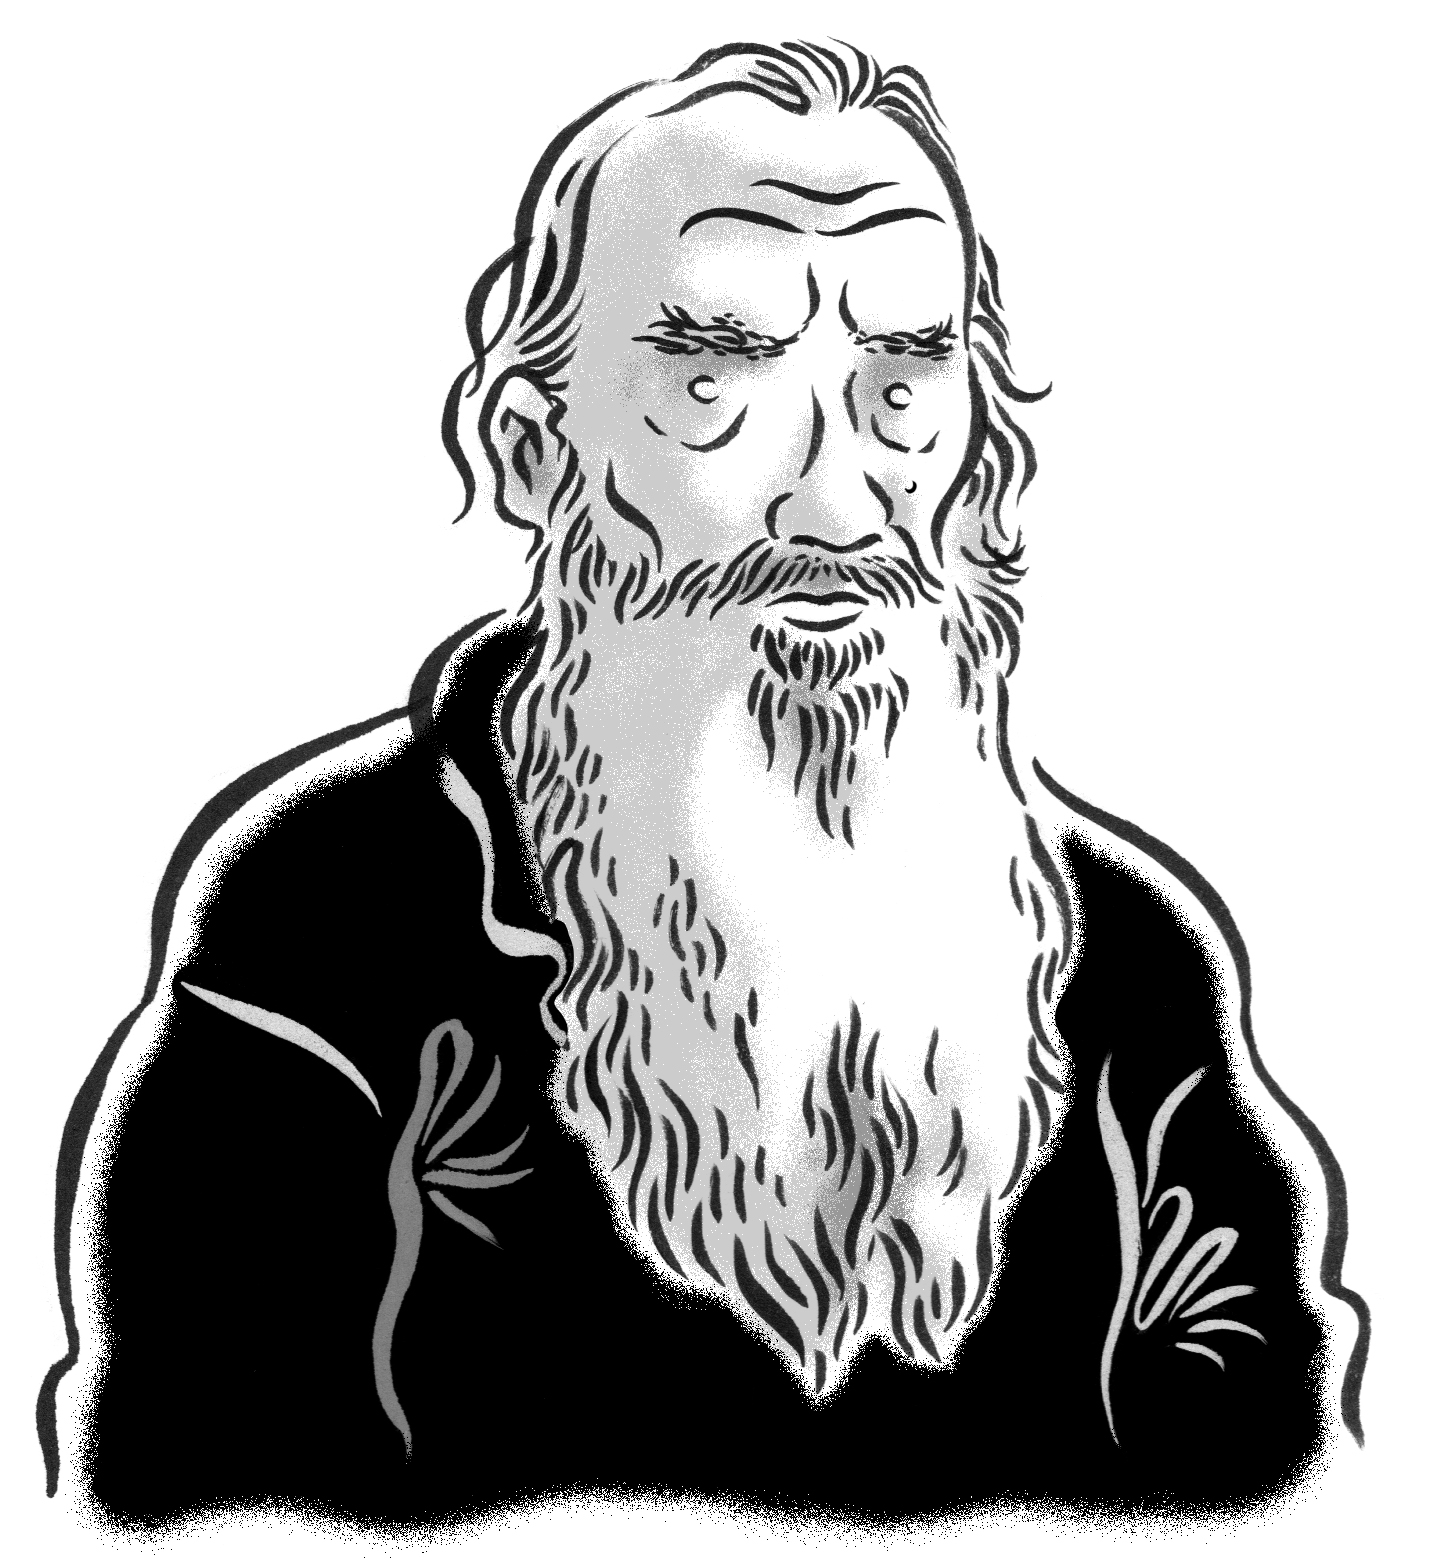
\includegraphics[width=6cm]{./imgs/autor4.jpg}
\end{center}


\chapter{O prisioneiro do cáucaso \subtitulo{(História verdadeira)}}

\section{1}

\noindent{}Um fidalgo servia no Cáucaso como oficial. Seu nome era Jílin.

Um dia, chegou uma carta de casa. A velha mãe lhe escrevia: ``Já estou
velha e quero ver o filho amado antes de morrer. Venha se despedir,
enterre"-me e depois volte com Deus para o serviço militar. Também
encontrei uma noiva para você: é inteligente, boa e tem posses. Se você
gostar dela, case e fique de vez''.

Jílin refletiu: ``De fato: a velha já está mal; talvez eu nem consiga
vê"-la. Eu vou e, se a noiva for boa, posso até casar''.

Foi ao coronel, tirou licença, disse adeus aos camaradas, ofereceu
quatro baldes de vodca a seus soldados na despedida e se preparou para
partir.

O Cáucaso, nessa época, estava em guerra.\footnote{A Guerra do Cáucaso
  (1817--1864), muito retratada na literatura russa do séc. \textsc{xix},
  envolveu uma série de conflitos, resultando na anexação, por parte do
  Império Russo, do norte do Cáucaso.} Não havia como passar pelas
estradas, nem de dia nem de noite. Bastava um russo sair da fortaleza, a
pé ou a cavalo, e os tártaros o matavam ou o levavam para as montanhas.
Estabeleceu"-se que, duas vezes por semana, uma escolta de soldados ia de
fortaleza em fortaleza. À frente e atrás iam soldados e, no meio, civis.

Era verão. Os comboios da fortaleza se reuniram ao amanhecer, os
soldados da escolta saíram e marcharam pela estrada. Jílin andava a
cavalo e a telega com suas coisas seguia com o comboio.

Havia vinte e cinco quilômetros a percorrer. O comboio ia devagar; ora
os soldados se detinham, ora a roda de alguma carroça soltava, ora um
cavalo empacava, e todos paravam e esperavam.

Já tinha passado do meio"-dia e o comboio só percorrera metade do
caminho. Areia, calor, sol pelando, e não havia onde se esconder. A
estepe nua, nem uma arvorezinha ou um arbusto à vista.

Jílin, à frente, se deteve e esperou a chegada do comboio. Ouviu um
toque de clarim --- pararam de novo. Ele pensou: ``Por que não vou
sozinho, sem os soldados? Minha égua é excelente; se os tártaros
atacarem, eu fujo. Vou ou não vou?\ldots{}''.

Parou, refletiu. E dele se aproximou outro oficial a cavalo, Kostýlin,
com uma espingarda, e disse:

--- Vamos sozinhos, Jílin. Não suporto mais, quero comer, e ainda este
calor de rachar. Minha camisa está ensopada.

Kostýlin, que era um homem corpulento e gordo, estava todo vermelho e
suava em bicas. Jílin pensou e perguntou:

--- A espingarda está carregada?

--- Está.

--- Pois então vamos. Com uma condição: não devemos nos separar.

E seguiram adiante pela estrada. Iam pela estepe conversando e olhando
para os lados. Ao redor, podia"-se ver longe.

Assim que a estepe acabou, a estrada passou por um desfiladeiro entre
duas montanhas. Jílin disse:

--- É preciso subir a montanha e olhar antes; eles podem aparecer por
trás dela, sem vermos.

Mas Kostýlin disse:

--- Olhar o quê? Vamos em frente.

Jílin não lhe deu ouvidos.

--- Não --- disse ---, espere aqui embaixo, só darei uma olhada.

E conduziu o cavalo pela esquerda na direção da montanha. A égua era de
caça (Jílin pagara cem rublos pela potra em uma manada e a adestrara
sozinho); ela o carregou pela escarpa como se tivesse asas nos pés.
Subiram a galope e, na frente deles, num raio de um hectare, surgiram
tártaros montados --- cerca de trinta. Jílin os viu e virou"-se para
trás; os tártaros o viram e lançaram"-se em seu encalço, tirando as
espingardas dos coldres na cavalgada. Ele desceu a escarpa à rédea
solta, gritando para Kostýlin:

--- Saque a espingarda! --- e para sua égua falou em pensamento:
``Amiguinha, carregue"-me, não enganche a pata, não tropece, ou estamos
perdidos. Vou pegar a espingarda, não me entregarei''.

Mas Kostýlin, assim que viu os tártaros, em vez de esperar, saiu em
disparada para a fortaleza. Com o açoite, fustigava o cavalo ora de um
lado, ora de outro. Apenas através da poeira era possível ver a cauda do
animal se mexer.

Jílin percebeu que a coisa estava feia. A espingarda se fora e só com um
sabre não podia fazer nada. Fez a égua recuar, na direção dos soldados,
pensando em fugir. Viu que seis sujeitos cavalgavam para lhe cortar o
caminho. Seu cavalo era bom, mas os deles eram melhores, e cavalgavam
para lhe cortar o caminho. Ele começou a dar a volta, quis retornar, mas
a égua já tinha disparado, incontida, voando ao encontro deles. Ele viu
se aproximar um tártaro de barba ruiva montado em um cavalo cinza. O
homem gania e arreganhava os dentes, a espingarda em riste.

``Pois bem'', pensou Jílin, ``eu conheço esses diabos, se me pegam vivo,
colocam"-me num fosso e me açoitam. Não me entregarei com vida.''

Jílin, embora de pequena estatura, era audaz. Sacou o sabre e fez a égua
saltar para cima do tártaro ruivo, pensando: ``Ou o esmago com o cavalo,
ou corto sua cabeça com o sabre''.

Estava a um cavalo de distância do tártaro quando lhe deram um tiro de
espingarda por trás e acertaram a égua. Ela caiu no solo com todo o seu
peso, desabando em cima da perna do oficial.

Quis se levantar, mas dois tártaros fétidos já estavam sentados sobre
ele, torcendo"-lhe o braço para trás. Conseguiu soltar"-se e derrubou os
tártaros, mas outros três apearam dos cavalos e se puseram a bater na
cabeça dele com coronhas. Os olhos dele toldaram e ele cambaleou.
Capturaram"-no, tiraram as cilhas sobressalentes da sela, prenderam"-lhe
com elas as mãos nas costas, atando"-as com um nó tártaro, e o arrastaram
até a sela. Derrubaram o chapéu de Jílin, tiraram"-lhe as botas,
revistaram tudo, tomaram o dinheiro e o relógio, e rasgaram as roupas.
Ele olhou para sua égua. Sua querida amiga jazia de lado, do jeito que
havia caído, e somente batia as pernas no chão, sem conseguir se erguer;
na cabeça, ela tinha um buraco de onde jorrava sangue negro, que
irrigava quase um metro da areia ao redor.

Um tártaro se aproximou do animal e começou a tirar"-lhe a sela. Como a
égua ainda se debatia, ele sacou o punhal e a degolou. Da garganta dela
saiu um assobiou, ela estremeceu e morreu.

Os tártaros terminaram de tirar a sela e o arreio. O sujeito de barba
ruiva montou em seu cavalo, enquanto os outros colocaram Jílin em cima
da sela dele; o oficial, para que não caísse, foi amarrado com uma
correia ao cinturão do cavaleiro e levado para a montanha.

Jílin estava sentado atrás do tártaro, balançando e batendo o rosto nas
costas fétidas dele. Só via diante de si as costas robustas do tártaro,
seu pescoço musculoso e a nuca azulada e raspada debaixo do gorro. A
cabeça de Jílin estava ferida, sangue coagulou sobre os olhos. Ele não
tinha como se ajeitar em cima do cavalo, nem como enxugar o sangue. Os
braços estavam tão retorcidos, que lhe machucavam a clavícula.

Por muito tempo passaram de montanha em montanha, então cruzaram o vau
de um rio, saíram para a estrada e entraram em um vale.

Jílin queria observar o caminho, ver por onde o levavam, mas os olhos
continuavam sujos de sangue e ele não conseguia se virar.

Começou a escurecer. Atravessaram mais um riacho e começaram a subir uma
montanha pedregosa; cheirava a fumaça, cães ladravam.

Chegaram ao \emph{aul}.\footnote{\emph{Aul}, aldeia tártara.
  (Nota de Tolstói.)} Os homens apearam dos cavalos, crianças tártaras
se reuniram e cercaram Jílin, piando, alegrando"-se e atirando"-lhe
pedregulhos.

Um tártaro enxotou as crianças, tirou Jílin do cavalo e chamou um
criado. Veio um nogai\footnote{Nogai, povo de origem turcomana que
  vivia nas montanhas no norte do Cáucaso.} de zigomas salientes, usando
apenas uma camisa. Rasgada, a camisa deixava"-lhe o peito nu à mostra. O
tártaro deu"-lhe uma ordem. O criado trouxe um grilhão: dois cepos de
carvalho presos a anéis de ferro, e em um deles havia uma argola com um
cadeado.

Ao desamarrarem os braços de Jílin, colocaram"-lhe o grilhão, levaram"-no
a um celeiro, empurrando"-o lá, e trancaram a porta. O oficial caiu em
cima de esterco. Abatido, tateou no escuro para achar um lugar macio e
se deitou.

\section{2}

Jílin quase não dormiu aquela noite. As noites lá eram curtas. Viu por
uma fresta que começava a clarear. Ergueu"-se, alargou a fresta e se pôs
a observar.

Viu uma estrada que descia a montanha; à direita, uma
\emph{sáklia}\footnote{\emph{Sáklia,} casa dos montanheses do
  Cáucaso.} tártara com duas árvores ao lado. Um cachorro preto estava
deitado na soleira, uma cabra andava com seus cabritos agitando os
rabos. Viu subir a montanha uma tártara jovenzinha que vestia uma camisa
colorida sem cinto, calças e botas, e carregava sobre a cabeça coberta
por um cafetã\footnote{Usado pela proibição a mulheres muçulmanas de
  mostrarem o rosto.} um grande jarro de lata com água. Caminhava com as
costas arqueadas, tremendo, e levava pela mão um menininho tártaro de
cabeça raspada usando apenas uma camisa. A jovem chegou com a água à
\emph{sáklia}; o sujeito de barba ruiva da véspera saiu trajando um
\emph{bechmet}\footnote{\emph{Bechmet,} cafetã de colarinho alto,
  traje típico dos povos montanheses, depois adotado como parte do
  uniforme dos regimentos dos cossacos.} de seda, um punhal prateado na
cintura e sapatаs nos pés nus. Na cabeça, um gorro alto preto, de couro
de carneiro, deslocado para trás. Saiu, espreguiçou"-se e acariciou a
barba ruiva. Ali postado, deu uma ordem ao criado e foi para algum
lugar.

Depois apareceram dois meninos a cavalo vindos do bebedouro. Os cavalos
tinham as fuças molhadas. Vieram correndo outros garotos, de cabeça
raspada, só de camisa e sem calças; formaram um grupo, foram até o
celeiro, pegaram uma vara e a enfiaram na fresta. Jílin ergueu a voz: os
moleques gritaram com estridência e saíram correndo dali com os joelhos
nus brilhando.

Jílin queria tomar água, tinha a garganta seca; pensava que pelo menos
devesse se fazer notar. Aguçou os ouvidos --- estavam abrindo o celeiro.
Veio o sujeito ruivo acompanhado por outro tártaro, mais baixo,
moreninho. Olhos negros e brilhantes, rosto corado, barbicha bem
aparada; expressão alegre, sempre risonha. O traje do moreno era ainda
melhor: \emph{bechmet} azul de seda adornado com galões. O punhal da
cintura era grande, de prata; as sapatas vermelhas de marroquim também
tinham galões prateados. E, em cima das sapatas finas, usava outras,
mais grossas. Um gorro alto, branco, de pelo de carneiro.

O tártaro ruivo entrou, disse algo que parecia um xingamento e ficou ali
postado; o sujeito, apoiando"-se no batente da porta, mexia no punhal
olhando para Jílin de soslaio, como um lobo. O moreninho --- rápido,
vivo, como se fosse movido por uma mola --- foi direto até Jílin,
acocorou"-se, arreganhou os dentes e deu"-lhe um tapinha no ombro, então
balbuciou algo rápido no seu idioma, piscou os olhos e estalou a língua,
dizendo sem parar: ``\emph{bon"-russo}! \emph{Bon"-russo}!''.

Jílin nada compreendeu e disse: ``Beber, deem água para beber!''.

O moreno riu: ``\emph{Bon"-russo}'', continuando a balbuciar na sua
língua.

Jílin mostrou com os lábios e as mãos que queria beber.

O moreno entendeu, riu, olhou para a porta e chamou alguém: ``Dina!''.

Veio correndo uma moça, delicada, magrinha, de treze anos, parecida de
rosto com o moreno. Pelo visto, era a filha. Os mesmos olhos negros e
brilhantes, e bonita de rosto. Vestia uma camisa longa e azul, de mangas
largas, sem cinto, com costura em vermelho nas abas, no peito e nas
mangas. Nas pernas e nos pés, usava calças e sapatas e, em cima delas,
outras sapatas de salto mais alto; no pescoço, um colar todo feito de
moedas russas de cinquenta copeques. A cabeça descoberta\footnote{A
  obrigação de cobrir a cabeça entre as mulheres muçulmanas geralmente
  começa após o casamento.} tinha uma trança vermelha com uma fita em
que pendiam penduricalhos e um rublo de prata.

O pai lhe deu uma ordem. Ela saiu e voltou trazendo um jarrinho de lata.
Deu água ao russo, acocorou"-se e se arqueou de um jeito que os ombros
ficaram abaixo dos joelhos. Agachada e de olhos bem abertos, observava
Jílin bebendo como um animal.

Ele devolveu"-lhe o jarro, e ela saltou para trás, como uma cabra
selvagem. Até o pai riu. Deu"-lhe outra ordem. Dina pegou o jarro, saiu
correndo e voltou trazendo pão ázimo em uma pequena tábua redonda; então
sentou de novo, arqueada, sem tirar os olhos de Jílin.

Os tártaros saíram e trancaram a porta de novo.

Pouco depois, o nogai se aproximou de Jílin e disse:

--- Arre, patrão, arre!

Também não sabia russo. Jílin só entendeu que o estava mandando ir a
algum lugar.

Saiu com o grilhão, claudicando de uma perna, e, sem conseguir pisar,
virou o pé para o lado. Ia atrás do nogai. Viu a aldeia tártara, cerca
de dez casas e a igreja deles com uma torre. Em uma casa, havia três
cavalos selados. Meninos seguravam as rédeas. O tártaro moreno saiu de
lá e acenou para que Jílin fosse até ele. Riu, falando algo em sua
língua, e foi para dentro. Jílin entrou. O aposento era bom, com paredes
revestidas de argila lisa. Colchões coloridos de penas estavam apoiados
na parede em frente; nas laterais foram pendurados tapetes caros; nos
tapetes, espingardas, pistolas e sabres de prata. Perto de uma parede,
ficava uma pequena estufa construída no mesmo plano que o solo. O chão
era de terra, limpo como uma eira, e todo o canto da frente estava
coberto de feltro; sobre o feltro, havia tapetes com almofadas de penas.
Nos tapetes, estavam sentados tártaros usando sapatas: o moreno, o ruivo
e três convidados. Nas costas de todos colocaram almofadas e, diante
deles, uma tábua redonda com panquecas de painço, manteiga derretida de
leite de vaca num pote e cerveja tártara --- а \emph{buzá}\footnote{\emph{Buzá,}
  bebida adocicada e fermentada (de trigo, milho ou painço) de baixo
  teor alcoólico, consumida na Crimeia e no Cáucaso.} \emph{---} em um
jarrinho. Comiam com as mãos lambuzadas.

O moreno ergueu"-se de salto e mandou Jílin sentar"-se ao lado, não no
tapete, mas no chão duro, então voltou a sentar e regalou os convidados
com panquecas e \emph{buzá.} Um criado acomodou Jílin, então ele mesmo
tirou as sapatas de cima, colocou"-as junto à porta, onde os outros
calçados se enfileiravam, e se sentou sobre o feltro, mais perto do dono
da casa; ao ver como estavam comendo, começou a salivar.

Quando os tártaros terminaram de comer, apareceu uma tártara vestindo
uma camisa igual à da moça de antes e calças; tinha a cabeça coberta por
um lenço. Retirou a manteiga e as panquecas e trouxe uma boa selha e um
jarro de bico estreito. Eles se puseram a lavar as mãos, depois cruzaram
os braços, ajoelharam"-se, sopraram em todas as direções e rezaram.
Conversavam na língua deles. Então um dos convidados virou"-se para Jílin
e começou a falar em russo.

--- Você foi capturado por Kazi Muhammed --- disse ele e apontou para o
tártaro ruivo ---, que o deu para Abdul Murat --- apontou para o
moreninho. --- Abdul Murat agora é o seu dono.

Jílin ficou calado. Abdul Murat começou a falar, sempre apontando para
Jílin, rindo e dizendo: ``soldado \emph{bon"-russo, bon"-russo}''.

O tradutor redisse: ``Está mandando você escrever para casa atrás de um
resgate. Assim que o dinheiro chegar, você será solto''.

Jílin pensou e disse: ``E ele quer um resgate grande?''.

Os tártaros falaram e o tradutor repetiu:

--- Três mil rublos.

--- Não --- disse Jílin ---, não posso pagar isso.

Abdul ergueu"-se num pulo, começou a agitar os braços, disse algo a Jílin
como se este pudesse compreendê"-lo. O tradutor verteu: ``Quanto você
dará?''.

Jílin pensou e disse: ``Quinhentos rublos''.

Daí entre os tártaros levantou"-se um berreiro. Abdul se pôs a gritar com
o ruivo de maneira tão incompreensível e rápida, que salpicava saliva de
sua boca. E o ruivo só fazia semicerrar os olhos e estalar a língua.

Calaram"-se e o tradutor disse:

--- O patrão acha que quinhentos rublos de resgate é pouco. Ele pagou
duzentos rublos por você. Kazi Muhammed tinha uma dívida com ele. Ele
tomou você no lugar do acerto da dívida. Três mil rublos, não se pode
admitir menos. Se você não escrever, vão colocá"-lo num fosso e
castigá"-lo com o açoite.

``Ah!'', pensou Jílin, ``com esses aí, quanto mais me intimidar, pior
será''. Ficou de pé e disse:

--- Pois diga a esse cachorro que, se ele quiser me assustar, não darei
um copeque, nem escreverei para casa. Nunca tive e nunca terei medo de
vocês, cachorros!

O tradutor falou tudo aos tártaros e de novo se levantou uma gritaria.

Balbuciaram por muito tempo, até que o moreno se levantou de salto e se
aproximou de Jílin.

--- \emph{Bon"-russo} --- disse ---, \emph{djiguit, djiguit}!

\emph{Djiguit,} na língua deles, significa ``valente''.\footnote{\emph{Djiguit,}
  para os povos da Ásia Central e do Cáucaso, é um cavaleiro habilidoso
  e valoroso.} Ele riu, disse algo ao tradutor, que explicou:

--- Dê mil rublos.

Jílin não arredou pé: ``Mais de quinhentos rublos eu não darei. E, se me
matarem, ficarão de mãos abanando''.

Os tártaros começaram a discutir e mandaram o criado a algum lugar,
olhando ora para Jílin, ora para a porta. O criado voltou seguido de um
homem meio gordo, descalço e esfarrapado, também com um grilhão no pé.

Jílin, então, deu um ``ah'' --- reconheceu Kostýlin. Também tinha sido
capturado. Os dois foram colocados lado a lado e começaram a conversar;
os tártaros assistiam em silêncio. Jílin contou o que lhe ocorrera;
Kostýlin contou que seu cavalo empacara, a espingarda falhara e que o
próprio Abdul o havia alcançado e capturado.

Abdul ergueu"-se num pulo, apontou para Kostýlin e disse algo.

O tradutor explicou que eles agora pertenciam ao mesmo dono e que, quem
pagasse o resgate primeiro, seria solto primeiro.

--- Veja --- disse a Jílin ---, você fica irritado, mas o seu camarada é
pacífico; escreveu uma carta para casa, vão mandar cinco mil rublos.
Então será bem alimentado e não sofrerá ofensas.

Jílin disse:

--- Camarada, como quiser; ele pode ser rico, mas eu não sou. --- Eu ---
continuou ele --- farei o que disse. Podem me matar, se quiserem, mas
não vão tirar proveito disso, e escrever pedindo mais de quinhentos
rublos eu não vou.

Ficaram calados. De repente, Abdul deu um salto, pegou um bauzinho,
tirou uma pena, um pedaço de papel e um tinteiro e colocou tudo na
frente de Jílin, então bateu"-lhe no ombro e apontou: ``Escreva''. Havia
concordado com os quinhentos rublos.

--- Espere um pouco --- Jílin disse ao tradutor. --- Diga a ele que nos
alimente bem, que dê roupas e calçados decentes e não nos separe,
ficaremos mais felizes assim, e que tire o grilhão.

Olhou para o dono da casa e riu. Este também riu. Terminou de ouvi"-lo e
disse:

--- As melhores roupas eu darei: \emph{tcherkeskas}\footnote{\emph{Tcherkeska,}
  espécie de cafetã que se disseminou por todo o Cáucaso.} e botas tão
boas, que poderiam casar com elas. Serão alimentados como príncipes.
Querem morar juntos, que morem no celeiro. Mas o grilhão não tiro; vocês
fugirão. Tiro só de noite --- ergueu"-se e deu"-lhe um tapa no ombro. ---
\emph{Bon} para Ivan, \emph{bon} para Abdul!

Jílin escreveu a carta, mas colocou o endereço errado, para que ela não
chegasse ao seu destino. Pensava consigo: ``Vou fugir''.

Conduziram Jílin e Kostýlin ao celeiro, levaram para lá palha de milho,
um jarro de água, pão, duas \emph{tcherkeskas} velhas e botas gastas de
soldado. Pelo visto, tinham sido arrancadas de soldados mortos. À noite,
tiraram"-lhes os grilhões dos pés e trancaram o celeiro.

\section{3}

Jílin e seu camarada viveram assim um mês inteiro. O dono da casa
gracejava sempre. ``\emph{Bon} para Ivan; \emph{bon} para Abdul.'' Mas
os alimentava mal, só dava pão ázimo de farinha de painço, panqueca
rústica assada, e uma espécie de massa sem cozimento.

Kostýlin escreveu para casa mais uma vez, esperava o tempo todo pelo
envio de dinheiro e se aborrecia. Passava os dias no celeiro contando as
horas para a carta chegar ou dormindo. Mas Jílin sabia que sua carta não
chegaria e não escreveu outra.

``Onde minha mãe arranjaria tanto dinheiro para pagar por mim?'',
pensava ele. ``Ela vivia do que eu mandava. Se tiver que arrumar
quinhentos rublos, vai se arruinar de vez. Se Deus quiser, escaparei
daqui.''

E tudo observava, tentando descobrir uma forma de escapar. Às vezes
caminhava assoviando pelo \emph{aul}; às vezes se sentava para fazer
algum trabalho manual --- modelava uma boneca de argila ou trançava um
cesto de vime. Jílin era mestre em trabalhos manuais.

Uma vez, forjou uma boneca com nariz, braços e pernas e uma camisa
tártara e colocou"-a no telhado.

As tártaras saíram para buscar água. Dina, a filha do dono, avistou a
boneca e chamou as outras meninas. Largaram as jarras, olharam, riram.
Jílin pegou a boneca e esticou para elas. Todas riram, mas não se
atreveram a pegá"-la. Ele deixou a boneca ali, foi para o celeiro e ficou
olhando para saber o que aconteceria.

Dina veio correndo, lançou um olhar ao redor, pegou a boneca e fugiu.

No dia seguinte, ao amanhecer, Dina apareceu na soleira com a boneca.
Ela a tinha envolvido em retalhos vermelhos e a embalava como um bebê,
ninando"-a em sua língua. Uma velha surgiu, ralhou com a menina, pegou o
brinquedo e o quebrou,\footnote{No Islã, é proibido retratar ou
  esculpir imagens de seres humanos.} mandando"-a ir trabalhar.

Jílin fez outra boneca, ainda melhor, e deu à Dina. Ela trouxe um jarro,
pousou"-o no chão e sentou"-se. Então olhou risonha para o oficial
apontando para o jarro.

``O que há de engraçado?'', pensou Jílin. Ele pegou o jarro e pôs"-se a
beber. Pensou que fosse água, mas era leite. Bebeu e disse: ``que bom''.
Como Dina ficou contente!

--- Bom, Ivan, bom! --- e ela se ergueu num pulo, batendo palmas,
agarrou o jarro e saiu correndo.

\begin{figure}%[ht!]
\vspace*{-1.6cm}
\hspace*{-1.8cm}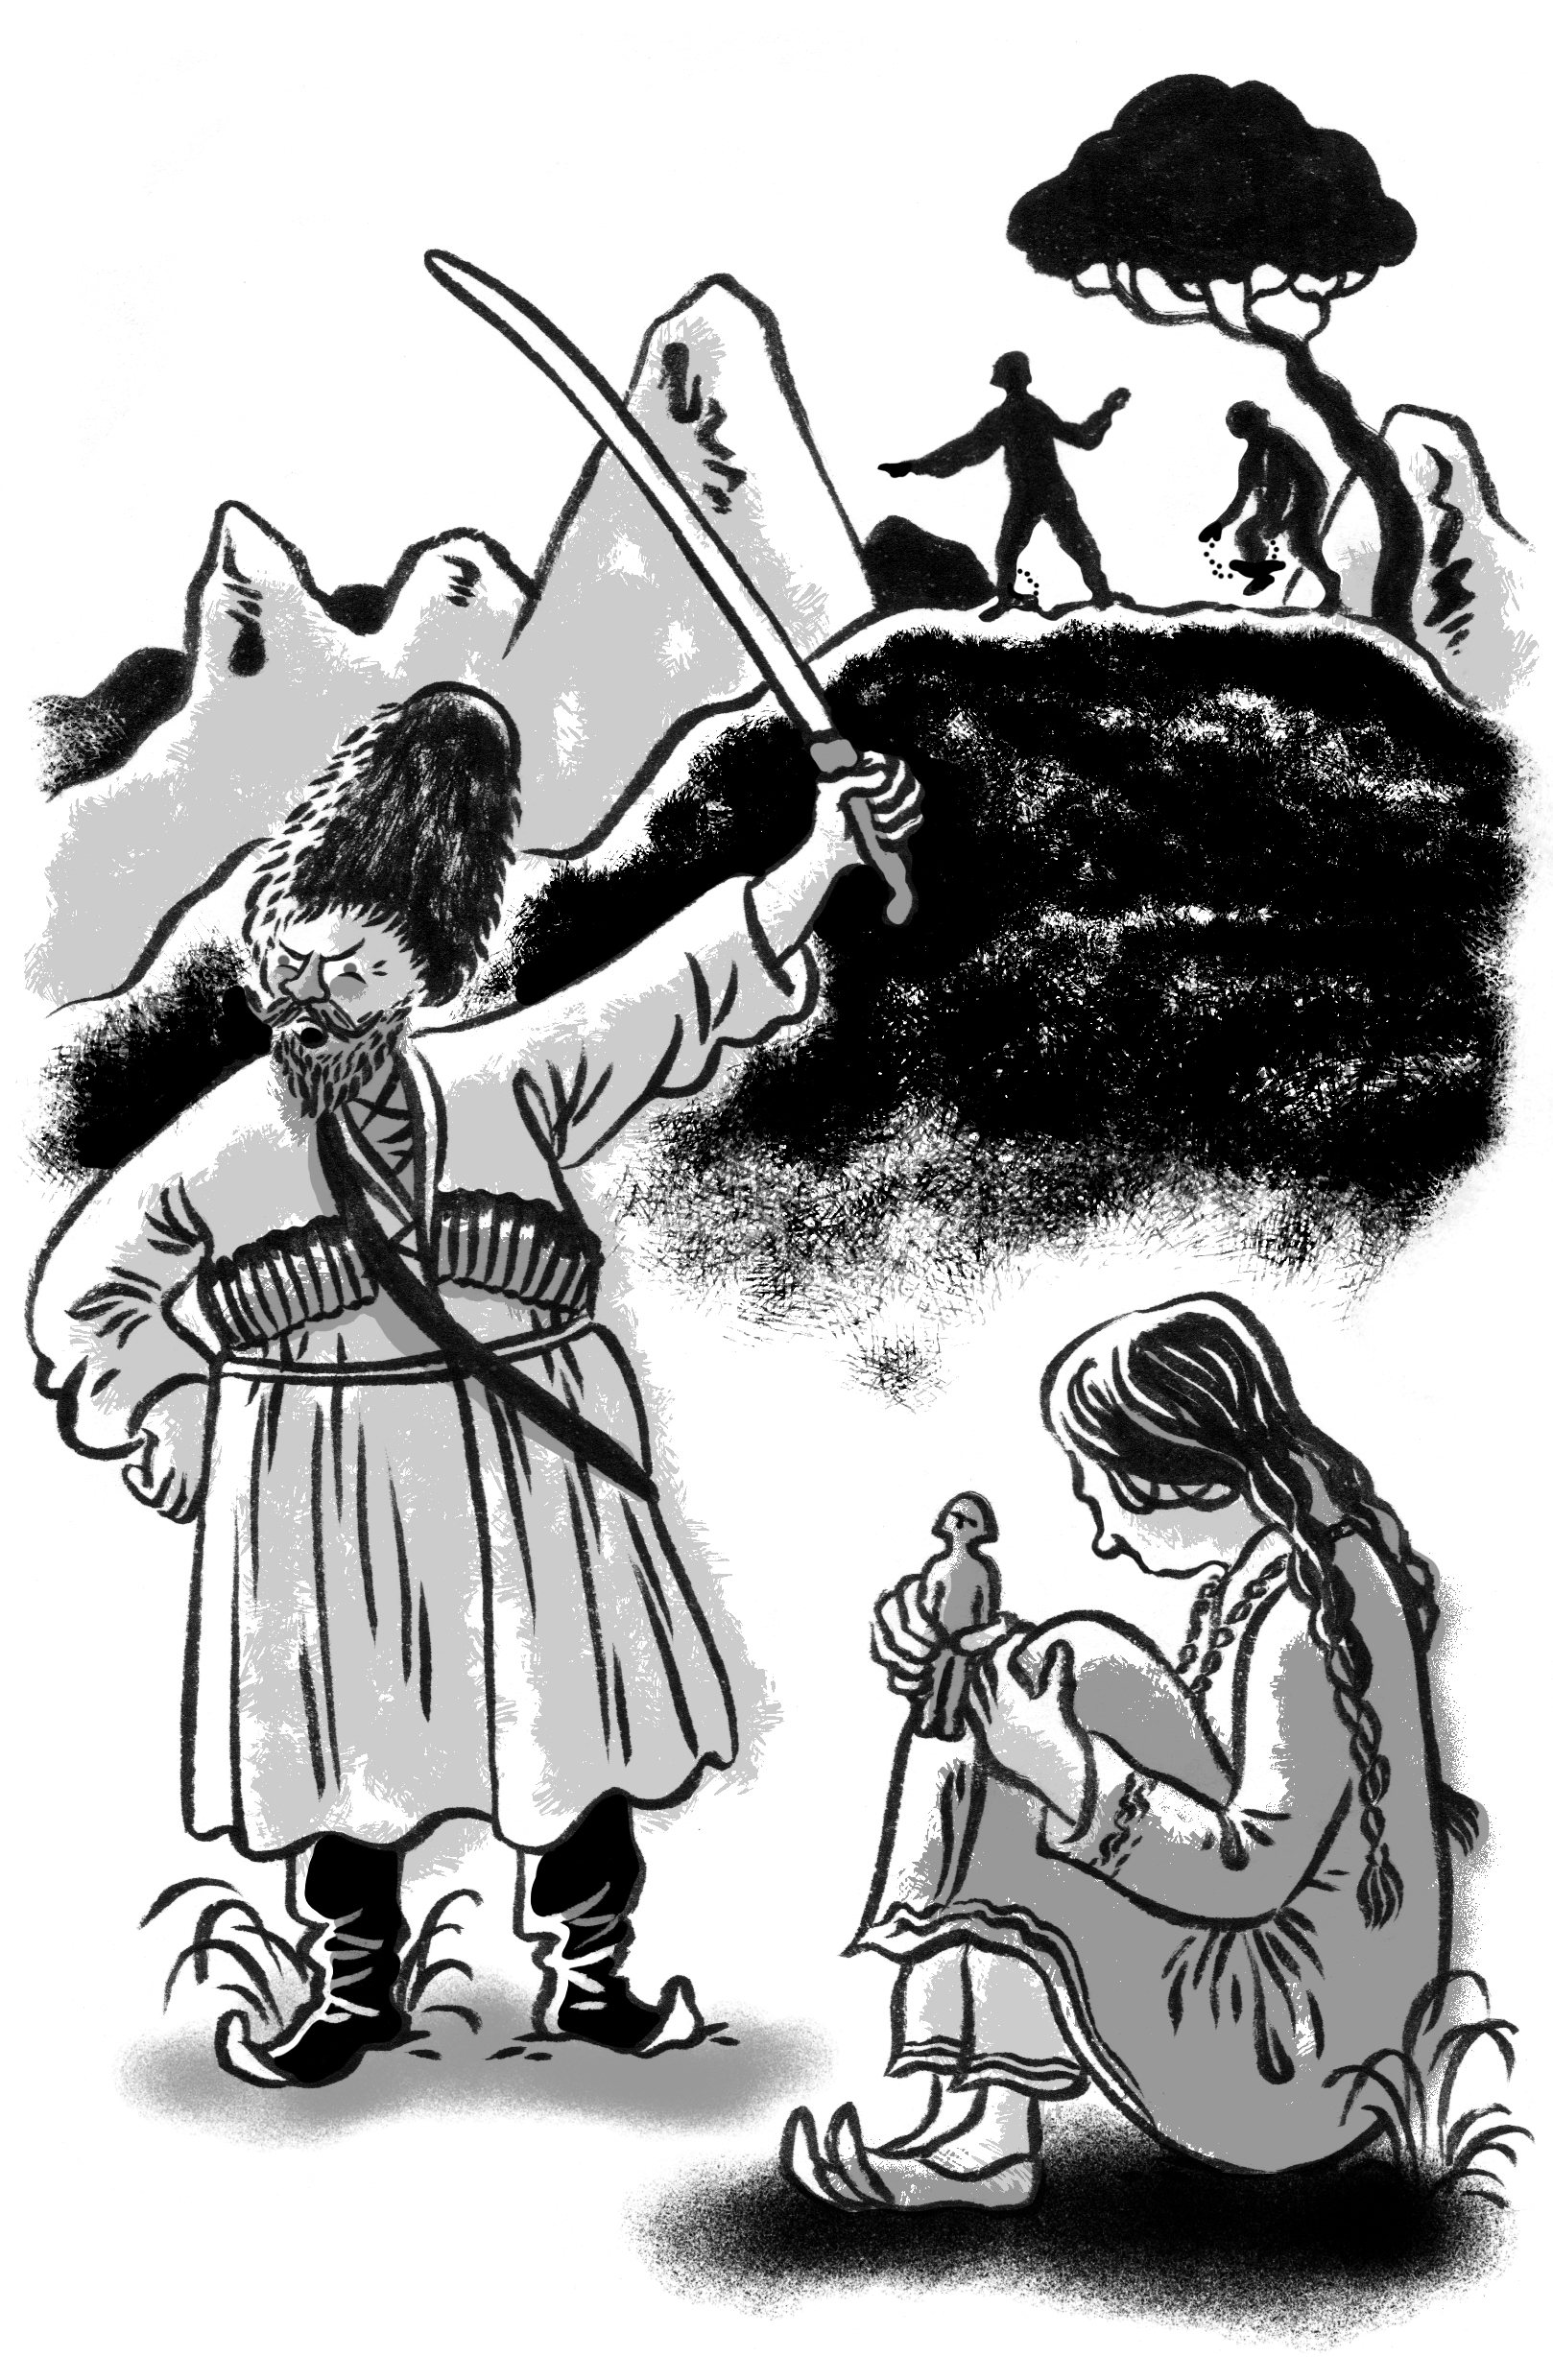
\includegraphics{./imgs/cena4.jpg}
\end{figure}

Desde então, ela passou a lhe dar leite, na surdina, todo dia. Quando os
tártaros fizeram panquecas de queijo de leite de cabra, que secavam nos
telhados, ela as trouxe em segredo ao oficial. E, da vez em que seu pai
abateu um carneiro, ela levou na manga um pedaço de carne para Jílin.
Largou"-o com ele e saiu correndo.

Um dia, houve uma tempestade forte, choveu a cântaros por uma hora.
Todos os riachos ficaram turvos; onde havia vau a água passou de dois
metros de altura e revirou pedras. Córregos fluíam em todo lugar, um
rumor pairava nas montanhas. Assim que passou o temporal, na aldeia
córregos começaram a correr por toda parte. Jílin pediu um canivete ao
dono da casa, esculpiu um pequeno eixo e tábuas para fazer uma roda, e
em cada lado da roda colocou um boneco.

As garotas levaram"-lhe retalhos e ele vestiu os bonecos: de mujique e de
camponesa, fixou"-os na roda e a colocou num córrego. A roda girava e os
bonecos saltavam numa dança.

A aldeia inteira se reuniu: meninos, meninas, mulheres; os tártaros
vieram, estalando as línguas:

--- Ah, \emph{bon"-russo}! Ah, Ivan.

Abdul tinha um relógio russo quebrado. Chamou Jílin, mostrou"-lhe,
estalou a língua. O oficial disse:

--- Está bem, eu conserto.

Pegou o relógio, abriu"-o com o canivete, desmontou"-o, montou"-o outra vez
e o entregou. O relógio estava funcionando.

O dono ficou contente, trouxe um \emph{bechmet} velho, todo em farrapos,
e deu a ele. Não havia como recusá"-lo --- ao menos serviria de coberta à
noite.

Desde então, Jílin levou fama de artesão. Vinham para vê"-lo de aldeias
distantes: um trazia a trava da espingarda ou da pistola para consertar,
outro o relógio. O dono forneceu"-lhe os apetrechos: pinças, verrumas e
limas.

Uma vez, adoeceu um tártaro e recorreram a Jílin: ``Vá, cure"-o''. Jílin
não sabia nada de medicina. Aproximou"-se, examinou o sujeito e pensou:
``Pode ser que sare sozinho''. Foi para o celeiro, pegou água e areia e
os misturou. Na frente dos tártaros, sussurrou algo sobre a água e a deu
ao doente. Por sorte, o tártaro se restabeleceu. Jílin passou a
compreender um pouco da língua deles. Alguns tártaros se habituaram a
ele --- quando era preciso, chamavam"-no: ``Ivan, Ivan!'' ---, e outros o
olhavam de soslaio, como para um animal feroz.

O ruivo não gostava de Ivan. Assim que topava com ele, franzia o cenho e
se afastava ou o insultava. Havia ainda um velho. Ele não morava no
\emph{aul,} mas vinha do sopé da montanha. Jílin só o via quando ele ia
fazer suas preces na mesquita. Era de baixa estatura, tinha um pano
branco enrolado no gorro, a barba e o bigode aparados e brancos como
neve, e o rosto enrugado e vermelho como tijolo. O nariz, em forma de
gancho, lembrava o bico do açor, os olhos eram cinzentos e raivosos, e
dos dentes só restaram os dois caninos. Andava com seu turbante, apoiado
em sua bengala, olhando ao redor como um lobo. Assim que via Jílin,
bufava e lhe dava as costas.

Um dia Jílin passou pelo sopé da montanha e foi espiar a morada do
velho. Desceu por uma trilha, viu um jardinzinho com uma cerca de pedra
e, detrás da cerca, cerejeiras, damasqueiros e uma isbá de teto plano.
Chegou mais perto; viu colmeias de palha trançada e abelhas voando e
zunindo. E o velho estava de joelhos, ocupado com algo numa colmeia.
Jílin subiu para olhar e o grilhão rangeu. O velho deu uma olhada e
ganiu; tirou a pistola da cintura e disparou na direção do intruso. Este
conseguiu por pouco proteger"-se atrás de uma pedra.

O velho foi se queixar ao dono, que chamou Jílin, riu e perguntou:

--- Para que foi à casa do velho?

--- Eu --- disse ele --- não lhe fiz nada de mal. Queria ver como vive.

O dono transmitiu"-o. Mas o velho, irritado, chiou, balbuciou algo,
mostrou os caninos e agitou os braços para Jílin.

Ele não compreendeu tudo, mas entendeu que tinha mandado seu dono matar os
russos em vez de mantê"-los no \emph{aul.} O velho foi embora.

Jílin quis saber quem era e perguntou ao seu dono, que explicou:

--- É um grande homem! Foi o primeiro \emph{djiguit,} matou muitos
russos, era rico. Tinha três mulheres e oito filhos. Todos moravam na
mesma aldeia. Vieram os russos, arrasaram a aldeia e mataram sete
filhos. O que sobrou se entregou a eles. Daí o velho também se entregou.
Morou três meses com os russos, encontrou o filho, matou"-o e fugiu.
Desde então, parou de guerrear e foi para Meca rezar a Deus. Por isso o
turbante. Quem esteve em Meca é chamado de \emph{hadji} e usa turbante.
Ele não gosta dos seus irmãos. Mandou matá"-lo; mas não posso, paguei por
você e gosto de você, Ivan; nem o deixaria partir se não tivesse dado a
palavra, que dirá matá"-lo --- riu e disse em russo: ``\emph{bon} para
Ivan, \emph{bon} para Abdul!''.

\section{4}

Jílin passou o mês assim: de dia caminhava pelo \emph{aul} ou se ocupava
com trabalhos manuais e, quando anoitecia e a aldeia sossegava, cavava
no chão do celeiro. Era difícil cavar por causa das pedras, mas ele as
triturava com ajuda da lima --- abriu um buraco debaixo da parede
através do qual conseguia perfeitamente passar. ``Só preciso conhecer
bem o lugar, descobrir para que lado ir. Nenhum tártaro me dirá isso'',
pensava ele.

Então escolheu um dia em que o dono estava fora e saiu do \emph{aul} depois do almoço 
na direção da montanha --- de lá queria observar o local.
Mas, antes de Abdul sair, tinha mandado seu filho ir atrás de Jílin e
não o perder de vista. O menino correu atrás dele e gritou:
--- Não vá! Papai não deixa. Vou chamar todo mundo agora mesmo.

Jílin pôs"-se a persuadi"-lo.

--- Eu não vou longe --- disse ele ---, só vou subir aquela montanha:
preciso encontrar uma erva para tratar seu povo. Venha comigo; com o
grilhão não vou escapar. E amanhã faço um arco e umas flechas para você.

Convenceu o pequeno e eles se foram. Ao olhar para a montanha, ela não
parecia tão distante, mas era difícil se locomover com o grilhão; ele
andou, andou, escalou"-a com muito custo. O oficial sentou e começou a
examinar o local. No sul, atrás da montanha, viu uma ampla ravina com um
rebanho pastando e, na parte de baixo, outro \emph{aul}. Para além
dele, havia outra montanha, mais íngreme, e depois dela ainda
outra. Entre elas, um bosque brilhava com reflexos azuis e ali montanhas
se erguiam mais e mais. Mais altas do que todas e brancas como açúcar
surgiam as montanhas cobertas de neve. E uma delas pairava acima das
outras. De leste a oeste, sempre montanhas; aqui e ali, \emph{auls}
fumegavam em desfiladeiros. ``Pois bem'', pensou ele, ``esse é lado
deles''. Pôs"-se a olhar para o lado russo: a seus pés, um riacho, o
\emph{aul} onde morava, jardins em volta. No riacho, pequenas
como bonecas, viu mulheres enxaguando roupa. Atrás do \emph{aul,}
embaixo, divisou uma montanha, depois dela mais duas e depois um bosque;
entre essas duas montanhas azulava uma planície, onde, ao longe, um fio
de fumaça se estendia. Jílin tentou se lembrar onde o sol nascia e onde
se punha quando morava na fortaleza. Olhou e teve certeza que naquele
vale ficava nossa fortaleza. Lá, entre aquelas duas montanhas, era por
onde tinha que fugir.

O sol começou a se pôr. As montanhas brancas nevadas ficaram vermelhas;
as montanhas escuras escureceram mais; névoa erguia"-se das amplas
ravinas e, ao cair do sol, o vale onde a fortaleza deveria estar parecia
em chamas. Jílin olhou atentamente e distinguiu algo que ao longe
parecia fumaça de chaminé. Então achou que era exatamente ali que a
fortaleza russa estava.

Tinha ficado tarde. Ouvia"-se o mulá\footnote{Mulá, clérigo islâmico.}
gritar. Tocavam o gado para casa, vacas mugiam. O menino chamava Jílin:
``vamos'', mas ele não tinha vontade de ir.

Finalmente voltaram para casa. ``Pois bem'', pensou Jílin, ``agora, que
conheço o lugar, preciso fugir.'' Queria partir nessa mesma noite. As
noites estavam escuras --- era lua minguante. Por azar, os tártaros
regressaram ao anoitecer. Normalmente vinham animados, conduzindo o
gado. Mas, dessa vez, não conduziam ninguém, mas traziam na sela um
tártaro morto, irmão do ruivo. Estavam zangados, prepararam"-se para
enterrá"-lo. Jílin saiu para ver. Envolveram o morto em um pano, sem
caixão,\footnote{Conforme o islamismo, os mortos não são enterrados em
  caixões e não se constroem mausoléus ou monumentos nos túmulos, para
  evitar ostentações.} levaram"-no para fora da aldeia, sob os plátanos,
e o colocaram sobre a relva. Veio o mulá, velhos se reuniram, enrolaram
panos nos gorros, tiraram os sapatos, e abaixaram"-se sobre os
calcanhares diante do morto.

À frente o mulá, depois três velhos de turbante, lado a lado, e atrás o
resto dos tártaros. Estavam agachados, com os olhos baixos e em
silêncio. Ficaram muito tempo calados. Então o mulá ergueu a cabeça e
disse:

--- Alá (quer dizer Deus)! --- disse somente essa palavra, então de novo
baixaram os olhos e silenciaram longamente, agachados, sem se mexerem. O
mulá voltou a erguer a cabeça:

--- Alá! --- e todos repetiram: ``Alá'', e se calaram outra vez.

O morto jazia na relva sem se mover, e eles estavam parados como mortos.
Nenhum deles se mexia. Só se ouviam as folhas do plátano reviradas pela
brisa. Depois o mulá leu uma prece, todos se levantaram, ergueram o
morto nos braços e carregaram"-no até uma cova. E não era uma simples
cova, fora escavada por baixo da terra como um porão. Pegaram o morto
debaixo do braço e pela batata da perna, dobraram"-no, baixaram"-no com
cautela, sentaram"-no debaixo da terra e colocaram as mãos dele sobre o
ventre.

Cobriram a cova com junco verde trazido pelo nogai, encheram"-na rápido
de terra, nivelaram"-na com a superfície e colocaram uma pedra em pé na
cabeceira do morto. Pisaram na terra e voltaram a se sentar alinhados
diante do túmulo. Ficaram muito tempo em silêncio.

--- Alá! Alá! Alá! --- por fim disseram, suspiraram e se levantaram.

Depois de distribuir dinheiro entre os velhos, o ruivo ergueu"-se, pegou
o açoite, golpeou"-se três vezes na testa e foi para casa.

Na manhã seguinte, Jílin viu o ruivo levando uma égua para fora da
aldeia, seguido por três tártaros. Saindo da aldeia, o ruivo tirou o
\emph{bechmet,} arregaçou as mangas --- os braços eram fortes ---, sacou
um punhal e o afiou na mó. Os tártaros ergueram a cabeça do animal, o
ruivo se aproximou, cortou"-lhe a garganta, derrubou a égua e começou a
esfolá"-la, tirando a pele com suas mãos grandes. Vieram mulheres e moças
e se puseram a lavar as tripas e as entranhas. Depois cortaram a égua e
levaram os pedaços para uma isbá. Toda a aldeia se reuniu na casa do
ruivo para rezar pela alma do morto.

Por três dias comeram a égua e beberam \emph{buzá} em memória do
defunto. Todos os tártaros ficaram em casa. No quarto dia, Jílin viu
que, na hora do almoço, preparavam"-se para ir a algum lugar. Trouxeram
cavalos, aprontaram"-se e partiram, uns dez homens, incluindo o ruivo; só
Abdul ficou. A lua era nova, e as noites ainda estavam escuras.

``Pois bem'', pensou Jílin, ``é preciso fugir agora'', e comunicou a
Kostýlin. Mas este se intimidou.

--- Mas como fugir? Nem sequer conhecemos o caminho.

--- Eu conheço o caminho.

--- Mas não chegaremos em uma noite.

--- Se não chegarmos, pernoitaremos na floresta. Eu peguei umas
panquecas. Para que quer ficar aqui parado? Se mandarem o dinheiro,
ficará bem; mas se não conseguirem mandar? E os tártaros agora estão
bravos, porque os russos mataram um deles. Dizem que querem nos matar.

Kostýlin pensou, pensou.

--- Então vamos.

\section{5}

Jílin se enfiou no buraco e o alargou para Kostýlin poder passar, e
ficaram esperando que o \emph{aul} sossegasse.

Assim que as pessoas do \emph{aul} silenciaram, Jílin meteu"-se debaixo
da parede, saiu do outro lado e sussurrou para Kostýlin: ``Venha''.
Kostýlin entrou no buraco, mas enroscou o pé em uma pedra e fez barulho.
E o dono tinha um vigia, um cão malhado, muito bravo e maldoso, que era
chamado Uliáchin. Jílin tinha dado comida a ele uma vez. Uliáchin ouviu
o barulho, começou a latir e a pular, seguido por outros cachorros.
Jílin deu um assobio baixo e jogou um pedaço de panqueca a Uliáchin, que
o reconheceu, abanou o rabo e parou de latir.

O dono ouviu e gritou da \emph{sáklia}: ``Quieto! Quieto! Uliáchin!''.

Mas Jílin já estava acariciando as orelhas dele. O cachorro
estava calado, esfregando"-se nas pernas do oficial e abanando o rabo.

Ficaram sentados atrás do celeiro. Tudo se acalmou: só se ouvia uma
ovelha balindo no curral e, abaixo, a água murmurando pelos pedregulhos.
Estava escuro; as estrelas pairavam alto e, sobre a montanha, a lua nova
enrubescia, com as pontas viradas para cima. No vale, a neblina era
branca como leite.

Jílin levantou"-se e disse ao camarada: ``Pois bem, meu velho, vamos!''.

Partiram; assim que se puseram em movimento, ouviram o mulá cantando no
telhado: ``Alá! \emph{Bismillah}! \emph{Al"-Rahman}!''.\footnote{\emph{Bismillah},
  ``em nome de Alá''; \emph{Al"-Rahman}, um dos nomes de Alá.}
Significava que estavam indo para a mesquita. Sentaram"-se de novo,
escondendo"-se atrás de um muro. Aguardaram muito tempo o povo passar.
Voltou a fazer silêncio.

--- Vamos, que Deus nos acompanhe! --- fizeram o sinal da cruz e
partiram.

Atravessaram o pátio, desceram pela escarpa até o riacho e o cruzaram
indo na direção da ampla ravina. Uma neblina espessa pairava baixa,
enquanto estrelas brilhavam sobre suas cabeças. Jílin determinava pelas
estrelas a direção a seguir. A neblina fresca não dificultava a
caminhada, mas as botas gastas eram incômodas. Jílin tirou as suas,
jogou"-as fora e continuou descalço. Pulava de pedra em pedra, observando
as estrelas. Kostýlin ficou para trás.

--- Vá devagar --- disse ele ---, malditas botas, arrebentaram"-me os
pés.

--- Pois tire, será mais fácil.

Kostýlin continuou a marcha descalço e foi ainda pior; machucava os pés
nas pedras e ficava sempre para trás. Jílin disse:

--- Se esfolar os pés, eles cicatrizam; mas, se nos alcançarem, eles nos
matam, será muito pior.

Kostýlin não dizia nada, andava e gemia de vez em quando. Desceram a
ravina por muito tempo. Aguçaram os ouvidos: à direita, cachorros
ladravam. Jílin parou, olhou ao redor e subiu uma montanha tateando.

--- Ei --- disse ---, nos enganamos, fomos pela direita. Aqui é outro
\emph{aul,} vi da montanha; precisamos voltar e subir pela esquerda. O
bosque tem que estar lá.

Mas Kostýlin disse:

--- Espere um pouquinho, deixe"-me respirar, meus pés estão sangrando.

--- Ei, meu velho, vão cicatrizar; mais fácil ir pulando. Assim!

E Jílin deu marcha a ré, para a esquerda, para a montanha, para o
bosque. Kostýlin sempre se atrasava, cheio de ais e uis. O outro o
chamava com um psiu e continuava adiante.

Subiram a montanha. Lá estava o bosque. Entraram rasgando nos espinhos
as últimas roupas. No bosque, deram com uma trilha. Foram por ela.

--- Pare! --- ouviram"-se batidas de cascos soando na estrada.

Pararam, escutaram. Soou algo como um patear de cavalo e cessou.
Seguiram --- e de novo os cascos bateram. Eles pararam --- e as batidas
pararam. Jílin esgueirou"-se e viu algo imóvel num ponto iluminado da
estrada. Parecia um cavalo sem ser, tinha algo estranho em cima que não
lembrava uma pessoa. Ouviu um bufar. ``Que raio é isso?'' Jílin assobiou
baixinho --- a criatura saiu em disparada da estrada rumo ao bosque,
crepitando, voando como uma ventania, quebrando os galhos.

Kostýlin caiu de medo. E Jílin riu:

--- É um cervo. Está ouvindo como quebra os galhos com os chifres?
Ficamos com medo dele e ele com medo de nós.

Seguiram em frente. A constelação das Plêiades já começava a baixar, a
manhã não estava distante. Mas não sabiam para que lado ir. Jílin achava
que tinha sido trazido por aquele caminho e que estavam a uns dez
quilômetros de distância dos seus irmãos; mas nada indicava isso e de
noite não se distinguem as coisas. Saíram para uma clareira. Kostýlin
sentou"-se:

--- Faça o que quiser, mas eu não vou --- as pernas não obedecem.

Jílin tentou persuadi"-lo.

--- Não --- disse ---, não vou, não consigo.

Jílin irritou"-se, desistiu de persuadir e o xingou.

--- Então vou sozinho, adeus!

Kostýlin ergueu"-se num pulo e foi adiante. Percorreram quatro
quilômetros. A neblina do bosque estava mais espessa, não enxergavam um
palmo diante do nariz, e as estrelas já quase não eram visíveis.

De repente, ouviram um tropel de cavalos à frente. Ouviram as ferraduras
prendendo nas pedras. Jílin deitou"-se de bruços e pôs"-se a auscultar o
solo.

--- É isso, um cavaleiro está vindo em nossa direção.

Saíram correndo da estrada, agacharam"-se em um arbusto e esperaram.
Jílin se arrastou até a estrada e viu um tártaro a cavalo conduzindo uma
vaca e cantarolando. O tártaro passou por eles. Jílin voltou para perto
de Kostýlin.

--- Deus nos poupou; levante"-se, vamos.

Kostýlin quis se erguer e caiu.

--- Não consigo, meu Deus, não consigo; não tenho forças.

O homem roliço, pesado, cobria"-se de suor; gelado da neblina do bosque,
com os pés dilacerados, ele desabou. Jílin tentou levantá"-lo à força,
mas Kostýlin começou a gritar:

--- Ai, dói!

Jílin ficou petrificado.

--- Por que está gritando? Os tártaros estão perto --- ouça.

E pensou: ``Está mesmo um caco; que faço com ele? Não se deve largar um
camarada''.

--- Pois bem --- disse ele ---, levante"-se, monte nas minhas costas; se
você não consegue andar, eu o levo.

Colocou Kostýlin em cima de si, acomodou as mãos sob as coxas e foi para
a estrada com o camarada nas costas.

--- Só não me aperte a garganta, santo Deus --- suplicou ele. --- Segure
no ombro.

Kostýlin era pesado para Jílin --- seus pés também sangravam e ele
estava fatigado. Ele se curvava e se erguia em seguida, jogava o outro
para o alto, para ajeitá"-lo melhor nas costas, e seguia pelo caminho.

Pelo visto, o tártaro tinha escutado Kostýlin gritar. Jílin ouviu alguém
galopando atrás e o chamando na língua dos tártaros. Jogou"-se nos
arbustos. O tártaro sacou a espingarda, atirou --- não acertou ---, deu
um grito em sua língua e saiu galopando pela estrada.

--- Pois bem, meu velho --- disse Jílin ---, estamos perdidos. Esse
cachorro agora vai reunir os tártaros para nos perseguirem. Se não
percorrermos pelo menos três quilômetros, estamos perdidos

E pensou consigo sobre Kostýlin: ``Para que diabo inventei de carregar
esse peso? Sozinho, eu teria escapado há muito tempo''.

Kostýlin disse:

--- Vá sozinho, por que se arriscar por minha causa?

--- Não, não se deve abandonar um camarada.

Colocou"-o nos ombros de novo e continuou a andar. Percorreu cerca de um
quilômetro assim. Caminhava sempre pelo bosque, que parecia não ter fim.
Mas a neblina já começava a se dispersar, nuvens iam surgindo, e as
estrelas não eram mais visíveis. Jílin estava esgotado.

Chegou a uma fonte revestida de pedras junto à estrada. Parou e desceu
Kostýlin.

--- Vamos descansar --- disse ---, beber um pouco dessa água. Comer
panquecas. Não devemos estar longe.

Mal se inclinou para beber, ouviu um tropel atrás. Jogaram"-se para a
direita, nos arbustos, e ficaram deitados sob uma escarpa.

Ouviram vozes de tártaros; tinham parado no lugar em que os oficiais
desviaram da estrada. Os tártaros conversaram entre si e depois pareciam
instigar os cachorros para atacar. Algo estalou nos arbustos e um
cachorro desconhecido foi direto até os fugitivos. Parou e começou a
latir.

Uns tártaros se enfiaram ali, também desconhecidos, e capturaram os
dois, que foram amarrados, colocados em cima de cavalos e levados
embora.

Percorreram três quilômetros e encontraram Abdul acompanhado por dois
homens. Falaram algo em tártaro e transferiram aos cavalos dele os
russos, que foram conduzidos de volta ao \emph{aul.}

Abdul já não fazia seus gracejos e não disse uma palavra aos dois.

Chegaram ao \emph{aul} ao amanhecer e os fizeram sentar em plena rua. As
crianças correram para lá. Dando gritos, elas começaram a apedrejá"-los e
a açoitá"-los.

Os tártaros reuniram"-se num círculo, incluindo o velho do sopé da
montanha. Entabularam uma discussão. Jílin entendeu que decidiam o que
fazer com eles. Uns diziam que era preciso mandá"-los para longe, além
das montanhas, enquanto o velho afirmava: ``Devem morrer''. Abdul se
opunha: ``Dei dinheiro por eles, vou receber um resgate''. Mas o velho
retrucava: ``Eles não vão pagar, só causarão desgraças. E alimentar
russos é pecado. Matem e acabem com essa história''.

Dispersaram"-se. O dono foi até Jílin e disse:

--- Se não me mandarem o resgate em duas semanas, vou açoitá"-los para
valer. E, se tentarem fugir de novo, mato"-os como cachorros. Escrevam
uma carta, mas escrevam direito!

Levaram papel aos dois, que escreveram as cartas. Colocaram"-lhes os
grilhões e os conduziram para trás da mesquita. Lá havia um fosso de
mais de três metros de profundidade, aonde os baixaram.

\section{6}

A vida de Jílin e Kostýlin ficou muito difícil. Não lhes tiravam os
grilhões, nem os deixavam sair ao ar livre. Jogavam ao fosso massa sem
cozimento, como se fossem dois cachorros, e baixavam jarros de água. Ali
dentro, o ar era fedorento, abafado e úmido. Kostýlin adoeceu muito,
inchou, doíam"-lhe todos os ossos do corpo; quando não estava gemendo,
estava dormindo. Jílin desanimou, via que as coisas iam mal. E não sabia
como escapar dali. Quis começar a cavar uma passagem, mas não tinha onde
jogar terra; o dono viu e ameaçou matá"-lo.

Uma vez, estava de cócoras pensando com tristeza na vida em liberdade
quando, de repente, caiu uma panqueca direto no seu colo, depois outra,
e choveram cerejas. Ele olhou para cima e lá estava Dina. Ela olhou para
ele, riu e saiu correndo. Jílin pensou: ``Dina não ajudaria?''.

Limpou um lugarzinho, amassou barro e pôs"-se a modelar bonequinhos. Fez
pessoas, cavalos, cachorros, pensando: ``Assim que Dina vier, lançarei
para ela''.

Só que no dia seguinte Dina não veio. E Jílin ouviu um tropel de
cavalos: tártaros se reuniram perto da mesquita, discutiram, gritaram e
mencionaram os russos. E ouviu a voz do velho. Não entendeu ao certo,
mas deduziu que os russos estavam próximos e os tártaros temiam que
entrassem no \emph{aul} e não sabiam o que fazer com os prisioneiros.

Depois de conversar, foram embora. De repente, ouviu um farfalhar em
cima de si. Ele olhou: Dina estava de cócoras com os joelhos acima da
cabeça, inclinava"-se tanto que o colar com moedas balançava sobre o
fosso. Os olhinhos brilhavam como estrelas; ela tirou da manga duas
panquecas de queijo e as lançou para ele. Jílin as pegou e disse:

--- Por que ficou tanto tempo sem vir? Fiz uns brinquedos para você.
Estão aqui! --- e começou a jogá"-los para o alto, um por um.

Mas ela abanava a cabeça, sem olhar.

--- Não precisa --- disse ela e fez uma pausa, então sentou"-se e
continuou a falar: --- Ivan! Querem matá"-lo --- apontou com a mão para o
pescoço.

--- Quem quer me matar?

--- Meu pai, os velhos mandaram. E tenho pena de você.

Jílin disse:

--- Se tem pena, traga"-me uma vara comprida.

Ela abanou a cabeça, como que dizendo: ``Não posso''.

Ele juntou as mãos e começou a suplicar:

--- Dina, por favor! Traga, queridinha!

--- Não posso --- disse ela ---, vão descobrir, estão todos em casa ---
e foi embora.

À noite, Jílin ficou refletindo sobre o que aconteceria. Olhava o tempo
todo para cima. Estrelas podiam ser vistas, mas a lua ainda não tinha
saído. O mulá gritou, tudo silenciou. Jílin, quase cochilando, ainda
pensava: ``A menina está com medo''.

De repente, caiu barro sobre sua cabeça; ele olhou para cima e viu uma
vara comprida fincada na extremidade oposta. A vara agitou"-se um pouco,
começou a baixar e deslizou para dentro do fosso. Jílin ficou contente,
pegou"-a e a desceu --- era uma vara grande que ele já tinha visto no
telhado do dono.

Olhou para o alto: as estrelas brilhavam alto no céu e, sobre o fosso,
os olhos de Dina, como os de uma gata, cintilavam na escuridão. Ela
inclinou o rosto na beirada e sussurrou: ``Ivan, Ivan!'', agitando as
mãos diante do rosto, como se dissesse: ``Fale baixo''.

--- Que foi? --- disse Jílin.

--- Saíram todos, só ficaram duas pessoas em casa.

Jílin disse:

--- Bem, Kostýlin, vamos tentar pela última vez; eu o ajudo a subir.

Kostýlin não quis ouvir nem um pio sobre isso.

--- Não --- disse ---, para mim não há como sair daqui, está claro. Aonde vou se nem para me virar tenho forças?

--- Então adeus, não guarde rancor --- e se beijaram.

Jílin agarrou a vara, mandou Dina segurá"-la e começou a escalar. Caiu
duas vezes --- o grilhão atrapalhava. Kostýlin segurou"-o e ele conseguiu
sair à superfície. Com suas mãozinhas Dina puxou"-o pela camisa, com toda
a força, e riu.

Jílin pegou a vara e disse:

--- Ponha no lugar, Dina, senão darão pela falta dela e baterão em você.

Ela saiu arrastando a vara e Jílin foi para o sopé da montanha. Desceu
pela escarpa, pegou uma pedra afiada e tentou arrancar o cadeado do
grilhão. Mas o cadeado era firme, não tinha como quebrá"-lo, e
incomodava. Ouviu alguém descer correndo a montanha, saltitando ligeiro.
Pensou: ``Deve ser Dina de novo''. Ela se aproximou, pegou a pedra e
falou:

--- Deixe comigo.

Ficou de joelhos e tentou arrancar o grilhão. Mas as mãozinhas eram
finas como varetas e não tinham força. Ela largou a pedra e desatou a
chorar. Ele ocupou"-se de novo do cadeado, e Dina ficou ao lado, de
cócoras, apoiada no ombro dele. Jílin lançou um olhar ao redor e viu, à
esquerda, detrás da montanha, um clarão vermelho: era a lua surgindo.
``Pois bem'', pensou, ``antes que a lua apareça, preciso cruzar a grande
ravina e chegar ao bosque.'' Ergueu"-se e largou a pedra. Com grilhão ou
sem, ele tinha que ir.

--- Adeus --- disse ---, querida Dina. Vou me lembrar de você para
sempre.

Dina abraçou"-o e tateou"-o, procurando um lugar onde colocar panquecas.
Ele as pegou.

--- Obrigado --- disse ---, menina esperta. Agora quem fará bonecas para
você? --- e acariciou"-lhe a cabeça.

Ela caiu no choro, cobriu o rosto com as mãos e correu pela montanha,
saltitando como uma cabrita. Na escuridão, só se ouvia o tilintar dos
penduricalhos em suas tranças ao bater nas suas costas.

Jílin fez o sinal da cruz, segurou o cadeado do grilhão, para que ele
não retinisse, e foi pela estrada --- arrastava a perna e mantinha os
olhos fitos no clarão de onde a lua surgia. Reconheceu o caminho. Tinha
que andar reto por uns oito quilômetros. Devia chegar ao bosque antes
que a lua saísse por inteiro. Cruzou o rio e a luz atrás da montanha
ficou mais visível. Andando pela ampla ravina, olhava para o alto: ainda
não se podia ver a lua. O clarão reluzia e um lado da ravina ia ficando
mais iluminado. Uma sombra deslizava sob a montanha, aproximando"-se
dele.

Jílin caminhava mantendo"-se na sombra. Apressava"-se, mas a lua ia mais
rápido; à direita, cumes de montanhas brilhavam. Ele estava chegando
perto do bosque, e a lua se revelava atrás da montanha --- uma lua
branca e clara como o dia. Já podia discernir todas as folhas das
árvores. Nas montanhas, estava silencioso e claro, como se tudo tivesse
deixado de existir. Apenas se ouvia, embaixo, o riacho murmurar.

\textls[-10]{Jílin chegou ao bosque sem cruzar com ninguém no caminho. Escolheu um
lugarzinho escuro e sentou"-se para descansar.}

Descansou e comeu panquecas. Encontrou uma pedra e pôs"-se novamente a
bater no grilhão. Machucou as mãos, mas não o quebrou. Levantou"-se e
seguiu pelo caminho. Percorreu um quilômetro, ficou sem forças e com as
pernas doloridas. A cada dez passos ele parava. ``Não há o que fazer'',
pensava ele, ``vou me arrastar enquanto tiver forças. Se me sentar, não
me levanto mais. Não conseguirei chegar à fortaleza, mas, quando
amanhecer, eu me deitarei no bosque, passarei o dia lá e, de noite,
continuarei.''

Andou a noite inteira. Dois tártaros a cavalo apareceram, mas Jílin os
ouviu de longe e escondeu"-se atrás de uma árvore.

\textls[-8]{A lua começou a empalidecer e o orvalho a cair; estava perto de clarear
e Jílin não tinha chegado à margem do bosque. ``Pois bem'', pensou,
``vou dar mais trinta passos, aí entro no bosque e me sento.'' Deu
trinta passos e viu que o bosque tinha acabado. Saiu para a margem ---
tinha clareado completamente e, diante dos seus olhos, estavam a estepe
e a fortaleza, e à esquerda, encostados ao sopé da montanha, fogos
ardiam e se consumiam, fumaça se estendia, e pessoas contornavam as
fogueiras.}

Ele olhou atentamente e discerniu espingardas brilhando,
cossacos,\footnote{Cossacos, guerreiros que pertenciam a comunidades
  seminômades e habitaram várias regiões da Rússia, passando a servir ao
  regimento imperial no século \textsc{xix}.} soldados!

\textls[-30]{Jílin alegrou"-se, reuniu as forças que restavam e foi para o sopé da
montanha. E pensou: ``Deus me livre de encontrar um cavaleiro tártaro em
campo aberto; mesmo estando perto, não escaparei''.}

Mal pensou, à esquerda, em uma colina, viu três tártaros num raio de
dois hectares. Eles o avistaram e saíram ao seu encalço. O coração de
Jílin parou. Ele acenou os braços e gritou com todas as forças:

--- Irmãos! Socorro! Irmãos!

Os nossos cossacos os ouviram e dispararam a cavalo. Lançaram"-se em sua
direção, para cortar o caminho dos tártaros.

Os cossacos estavam longe e os tártaros perto. Jílin reuniu as últimas
forças, pegou o grilhão com a mão e correu ao encontro dos cossacos, sem
consciência de seus atos, fazendo o sinal da cruz e gritando:

--- Irmãos! Irmãos! Irmãos!

Havia cerca de quinze cossacos. Os tártaros se assustaram e, sem
alcançá"-lo, detiveram"-se. E Jílin saiu correndo na direção dos russos.

\textls[-8]{Os cossacos cercaram"-no e perguntaram quem era, que fazia, de onde
viera. Jílin estava fora de si, apenas chorava e dizia:}

--- Irmãos! Irmãos!

Soldados vieram correndo e rodearam Jílin; um lhe deu pão, outro cereais
cozidos, outro vodca, outro o cobriu com um capote, outro lhe quebrou o
grilhão.

Os oficiais o reconheceram e o levaram à fortaleza. Os soldados ficaram
contentes, velhos camaradas se reuniram ao redor de Jílin.

Ele contou tudo o que lhe ocorrera e disse:

--- E eu estava voltando para casar! Pelo visto, não quis o destino.

Jílin continuou servindo no Cáucaso. Kostýlin só foi resgatado depois de
um mês em troca de cinco mil rublos. Estava quase morto quando o
trouxeram.

\medskip

{\footnotesize\hfill\emph{Tradução: Irineu Franco Perpetuo.}}


\chapter*{}
\label{part5}
\thispagestyle{empty}

\begin{vplace}[1.5]
{\HUGES\hfill\textbl{NIKOLAI LESKÓV}}

{\LARGE\hfill\textlt(1831–1895)}
\end{vplace}

\pagebreak
\thispagestyle{empty}
\mbox{}
\vfill
\begin{center}
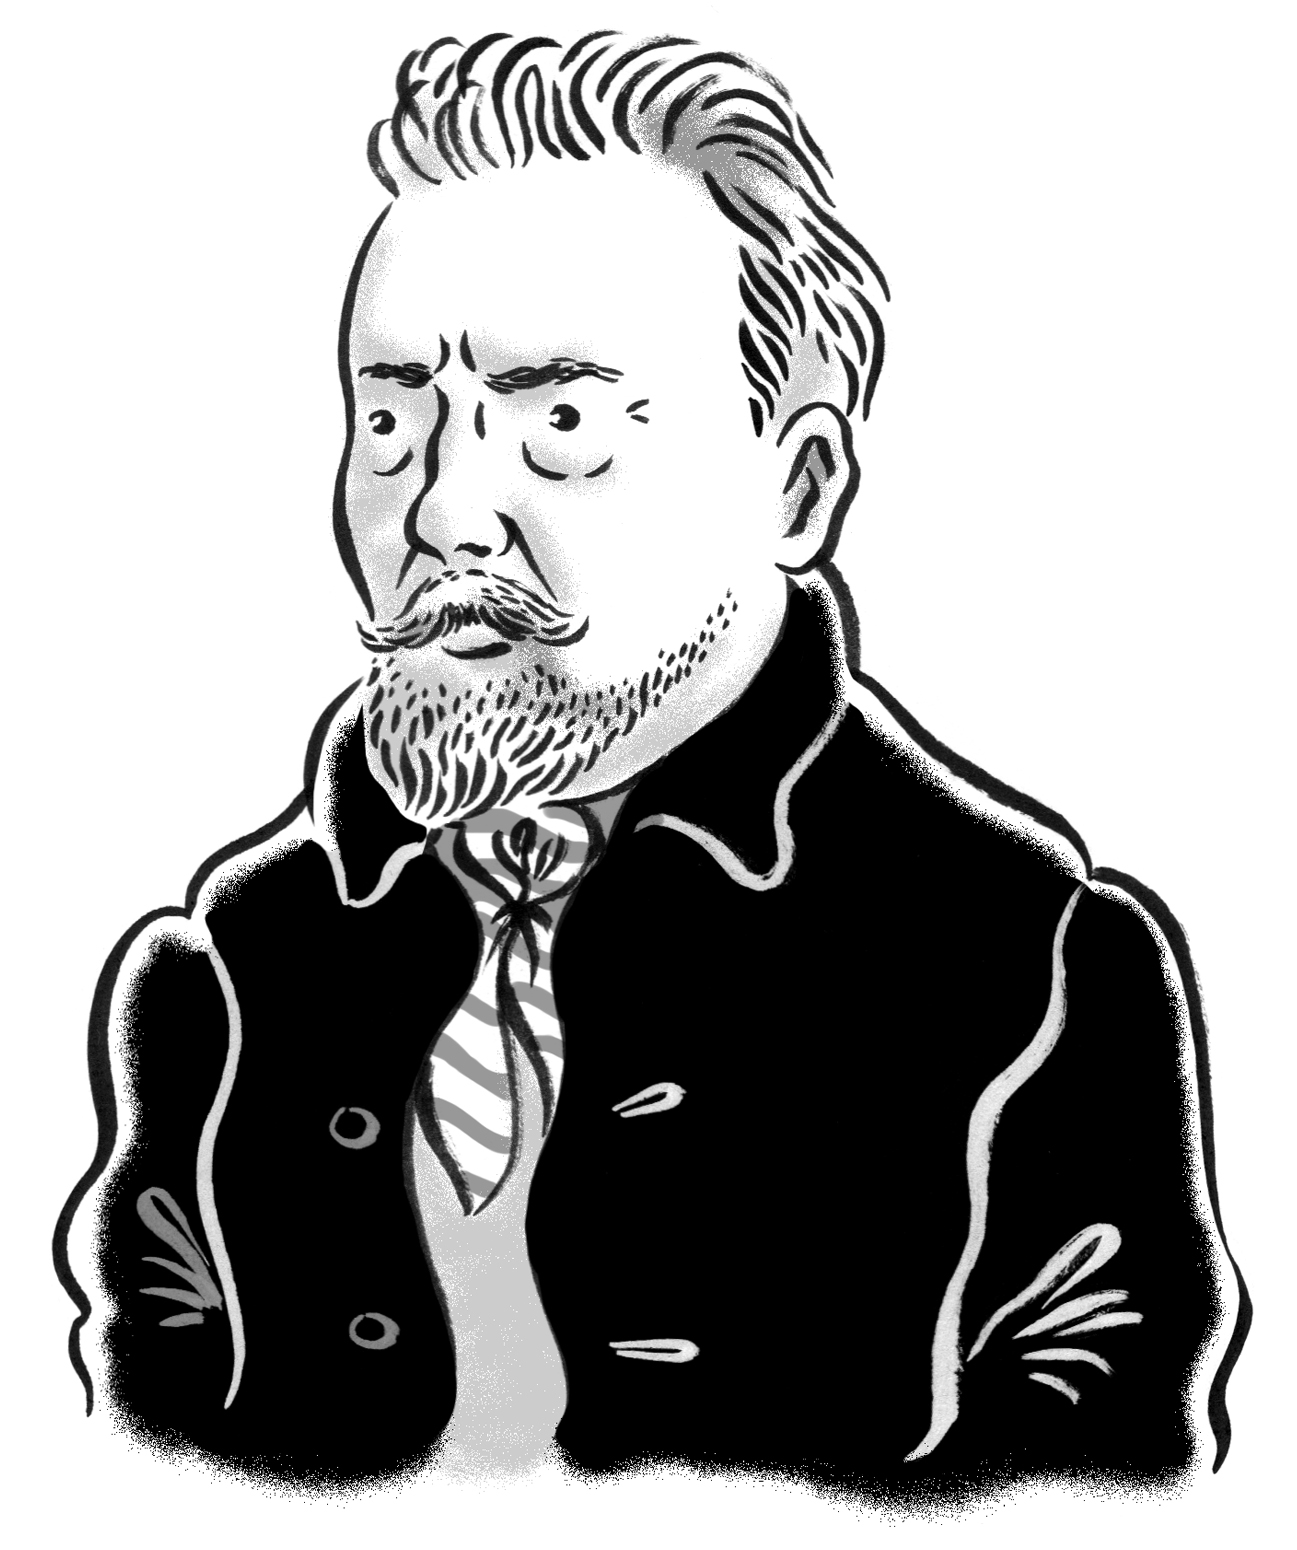
\includegraphics[width=6cm]{./imgs/autor5.jpg}
\end{center}


\chapter{Bobinho}

Quem deve ser considerado um bobo? Ao que parece, todo mundo sabe, mas,
se você se puser a verificar o que cada um entende por bobo, verá que as
pessoas não têm a mesma compreensão da bobice. Segundo o dicionário
acadêmico, em que cada palavra tem seu significado explicado, ``bobo é
um homem fraco do juízo, estúpido, desprovido de raciocínio, louco,
bufão''\ldots{} Para reforçar a explicação, é dado um exemplo literário:
``Ele foi e será o bobo dos bobos''. ``Bobinho é uma versão atenuada da
palavra \emph{bobo}.'' Não há para que buscar explicação mais
científica; contudo, na vida, acontece de encontrarmos bobos ou bobinhos
que receberam tal apelido, mas no fundo não são loucos, nem estúpidos,
nem têm nada de bufão\ldots{} São pessoas curiosas, e de uma delas vou falar.

Na nossa aldeia, havia um menino servo de pais desconhecidos chamado
Panka. Cresceu numa casa senhorial, vestia o que lhe davam e sentava à
mesa para comer com a ordenhadora e seus filhos. Sua função era ``ajudar
todo mundo''; isso significava que todos os trabalhadores da propriedade
tinham direito de obrigar Panka a fazer qualquer tarefa; dessa forma,
ele trabalhava sem parar. Agora assim ele me surge na memória: no
inverno --- e nossos invernos são rigorosos ---, quando nos levantávamos
e corríamos para a janela, Panka, curvado, já estava puxando trenós
grandes com feixes de feno, palha e cestos com espigas de cereais e
outros alimentos miúdos para o gado e as aves. Quando estávamos
acordando, ele já tinha se cansado de trabalhar e era visto raramente
--- ele ficava sentado no estábulo comendo um pedacinho de pão e tomando
água com uma concha de madeira.

Você perguntava a ele:

--- Panka, por que está mastigando pão seco?

E ele respondia com gracejos:

--- Como seco? Veja, é com água pura.

--- Você devia ter pedido algo mais: repolho, pepinos ou batatas!

E Panka sacudia a cabeça e respondia:

--- Ora, para quê?\ldots{} Já me empanturrei --- glória ao Senhor!

Punha o cinto e voltava para o pátio para carregar isso ou aquilo. Seu
trabalho não tinha fim, pois sempre alguém o forçava a ajudar em algo.
Limpava a estrebaria e o estábulo, dava comida ao gado, levava os ovinos
ao bebedouro e, à noite, trançava alpercatas para si e para os outros;
era o último a deitar e o primeiro a levantar, antes de amanhecer;
estava sempre vestido em farrapos. E ninguém tinha a menor pena dele, apenas
diziam:

--- Para ele, tanto faz --- é um bobinho.

--- Ele é bobinho em quê?

--- Em tudo\ldots{}

--- Por exemplo?

--- Quer exemplo? A ordenhadora dá todos os pepinos e as batatas para
seus filhos e nada para Panka, e para ele tanto faz\ldots{} Ele não pede para
ela, nem se queixa. Bobo!

Nós, crianças, não conseguíamos compreender isso muito bem e --- embora
nunca tivéssemos ouvido Panka dizer tolices e até sentíssemos carinho
por ele, porque nos fazia moinhos de brinquedo e cestinhos de bétula ---, como todos em casa, dizíamos igualmente que Panka não passava de
um bobinho, e ninguém discutia, mas logo aconteceu tal caso que discutir
sobre isso deixou de ser possível.

Tínhamos empregado um administrador geral severo, muito severo, que
gostava de castigar as pessoas por qualquer falta. Ia em um
\emph{drójki}\footnote{\emph{Drójki,} carruagem leve, aberta, de
  quatro rodas, usada para distâncias curtas.} ligeiro, olhando para
todos os lados à procura de negligência. E, se notava algo em desordem,
imediatamente parava, chamava o culpado e mandava:

--- Vá agora ao escritório e diga em meu nome ao supervisor que lhe deem
vinte e cinco varadas e, se não aparecer, à noite mando darem o dobro.

Ninguém ousava pedir perdão, pois ele não suportava isso e ainda
aumentava o castigo.

Uma vez, no verão, o administrador estava fazendo sua ronda quando viu
potros caminhando entre o cereal recém"-plantado, e eles não apenas
arrancavam a erva como pisoteavam e puxavam as raízes com os cascos\ldots{}

O homem saiu ralhando.

Os potros, nesse ano, tinham sido colocados sob guarda do menino
Petrucha,\footnote{Petrucha, apelido de Piotr.} filho da ordenhadora
Arina, a que negava batatas a Panka para dá"-las às suas crianças. O tal
Petrucha tinha, na época, doze anos e era muito menor e mais fino de
corpo do que Panka, motivo pelo qual era chamado, provocativamente, de
``ricotinha'' --- em suma, era um menino mimado pela mãe, fraco para o
trabalho e franzino para represálias. Depois de conduzir os potros de
manhã cedo ``para o orvalho'', começou a ter calafrios, cobriu"-se com
uma espécie de cafetã e, ao se aquecer, sentiu sono --- ele adormeceu e,
nessa hora, os potros foram até a plantação de cereais.

O administrador, ao ver isso, imediatamente deu um açoite em Petrucha e
disse:

--- Panka por enquanto vai cuidar das coisas dele e das suas, e você
agora vá até o posto de ordens e diga ao ajudante do supervisor para lhe
dar doze varadas; e, se até eu voltar para casa você não tiver cumprido,
de mim ganhará o dobro.

Disse e foi embora.

E Petrucha se debulhou em lágrimas. Tremia todo, pois nunca tinha sido
castigado com uma vara. Ele disse a Panka:

--- Panka, meu amigo, estou com muito medo\ldots{} Diga, o que devo fazer?

Panka acariciou"-lhe a cabeça e disse:

--- Eu também fiquei com medo\ldots{} Mas o que fazer?\ldots{} Bateram também em
Cristo\ldots{}

Petrucha chorou ainda mais amargamente e disse:

--- Tenho medo de ir e de não ir\ldots{} Melhor me jogar na água.

Panka se pôs a tranquilizá"-lo:

--- Ora essa: fique aqui de olho nas minhas coisas e nas suas, eu vou
correndo me empenhar por você --- talvez Deus tenha piedade. Veja como
você é medroso.

Petrucha perguntou:

--- Mas como você vai se empenhar, Panka?

--- Eu pensei numa coisa --- vou me empenhar!

E Panka saiu correndo lépido pelo campo, na direção da propriedade, e
uma hora depois voltou sorridente.

--- Não tema, Petrucha --- disse ---, está feito; não vá a lugar nenhum,
está livre do castigo.

Petrucha pensou: ``No fim das contas, tenho que acreditar nele'', e não
foi ao posto.

No dia seguinte, na isbá onde ficava o posto, o administrador perguntou
ao ajudante do supervisor:

--- E então, o pastorzinho veio apanhar ontem?

--- Como poderia não vir? --- disse o outro. --- Veio, Excelência.

--- Malharam o menino?

--- Sim --- o outro respondeu ---, malharam.

--- E bem?

--- Bem, com empenho.

A coisa sossegou, mas depois ficaram sabendo que não tinham surrado o
pastorzinho designado, Piotr, mas Panka, e a notícia correu a
propriedade e a aldeia: todos riram dele e o outro escapou da sova.

--- Que fazer? --- disseram. --- Mesmo que o bobo tenha ajudado, não se
vai castigar dois por um único pecado.

Pois então, nosso Panka não foi mesmo um bobo?

E assim ele continuou a viver.

Em alguns anos, estourou a guerra da Crimeia\footnote{A Guerra da
  Crimeia (1853--1856) envolveu, de um lado, o Império Russo e, de outro,
  a Inglaterra, a França e o Império Otomano. Nesse embate a Rússia
  perdeu parte da Bessarábia.} e começaram a convocar recrutas. O choro
percorreu a aldeia: ninguém tinha vontade de padecer na guerra. As mães,
especialmente, queriam matar"-se pelos filhos --- lamentavam um a um.

Panka, que nessa época já tinha chegado à idade adulta, aproximou"-se sem
aviso do dono da propriedade e solicitou: ``Mande'', disse ele, ``que me
levem à cidade para virar soldado''.

--- Que espécie de vontade é essa?

--- É isso --- respondeu ---, de repente me veio uma vontade grande.

--- Mas por quê? Repense.

--- Não --- disse ---, não há o que pensar.

--- Por que não?

--- O senhor não ouve como estão chorando ao redor? Eu sou amado apenas
por Deus, não há quem chore por mim, e quero partir.

Tentaram dissuadi"-lo.

--- Veja só como é desajeitado; na certa todos vão rir de você na
guerra.

E ele respondeu:

--- Melhor assim: rir é mais divertido do que brigar; se todos ficarem
felizes, farão as pazes.

Voltaram a lhe dizer:

--- O melhor é se consolar e ficar em casa!

Mas ele insistiu com firmeza.

--- Não --- disse ---, esse será o meu consolo.

Consolaram Panka, levaram"-no à cidade e o conduziram para o
recrutamento. Quando os emissários regressaram, todos começaram a
interrogá"-los com curiosidade:

--- Pois bem, como nosso bobo virou"-se por lá? Não o viram depois de o
entregarem?

--- Como não? --- disseram. --- Vimos, sim.

--- Por certo, riram da falta de jeito dele.

--- Sim --- disseram ---, riram no começo; daí, com os dois rublos que
lhe demos de gratificação, ele comprou travessas cheias de torta de
ervilha e de cereais cozidos, e as distribuiu entre todos, mas de si
mesmo esqueceu. Cada um se pôs a balançar a cabeça e a separar metade da
sua porção para ele. Mas ele ficou envergonhado e disse: ``O que é isso,
meus velhos, aqui não tem truque! Comam''. Os recrutas começaram a lhe
dar palmadinhas no ombro com amizade: ``Como você é amável!''. E, de
manhã, Panka levantou"-se antes de todos no quartel, arrumou tudo e
limpou as botas dos soldados veteranos. Os veteranos começaram a
elogiá"-lo e nos perguntaram: ``O que ele é, o bobo de vocês?''.

Os emissários responderam:

--- Bobo não, mas\ldots{} um pouco assim, de nascença.

Então Panka, com sua bobice, foi servir e passou a guerra inteira como
\emph{profos}\footnote{\emph{Profos,} no exército russo dos séculos
  \textsc{xviii} e \textsc{xix}, soldado ou suboficial encarregado de funções como a
  limpeza das instalações, supervisão dos presos e execução de sentenças
  de punição corporal.} --- escavava fossos e enterrava o lixo na
retaguarda ---; quando lhe deram baixa, por estar acostumado ao
pastoreio, foi contratado por tártaros da estepe para tomar conta de
manadas de cavalos.

Dirigiu"-se aos tártaros de Penza e ficou anos sem voltar, errando e
conduzindo cavalos, em um lugar distante perto do árido
Ryn"-Peski,\footnote{Ryn"-Peski é um deserto localizado a sudeste da
  República de Calmúquia (Rússia), a oeste do Cazaquistão e ao norte do
  mar Cáspio.} por onde, então, vagava o magnata local, Cã Djangar.
Quando ia vender cavalos em Sura, Cã Djangar portava"-se de forma
aparentemente dócil, porém, na sua estepe, fazia o que desse na telha:
punia ou dava privilégios a quem quisesse.

\begin{figure}%[ht!]
\vspace*{-1.6cm}
\hspace*{-1.8cm}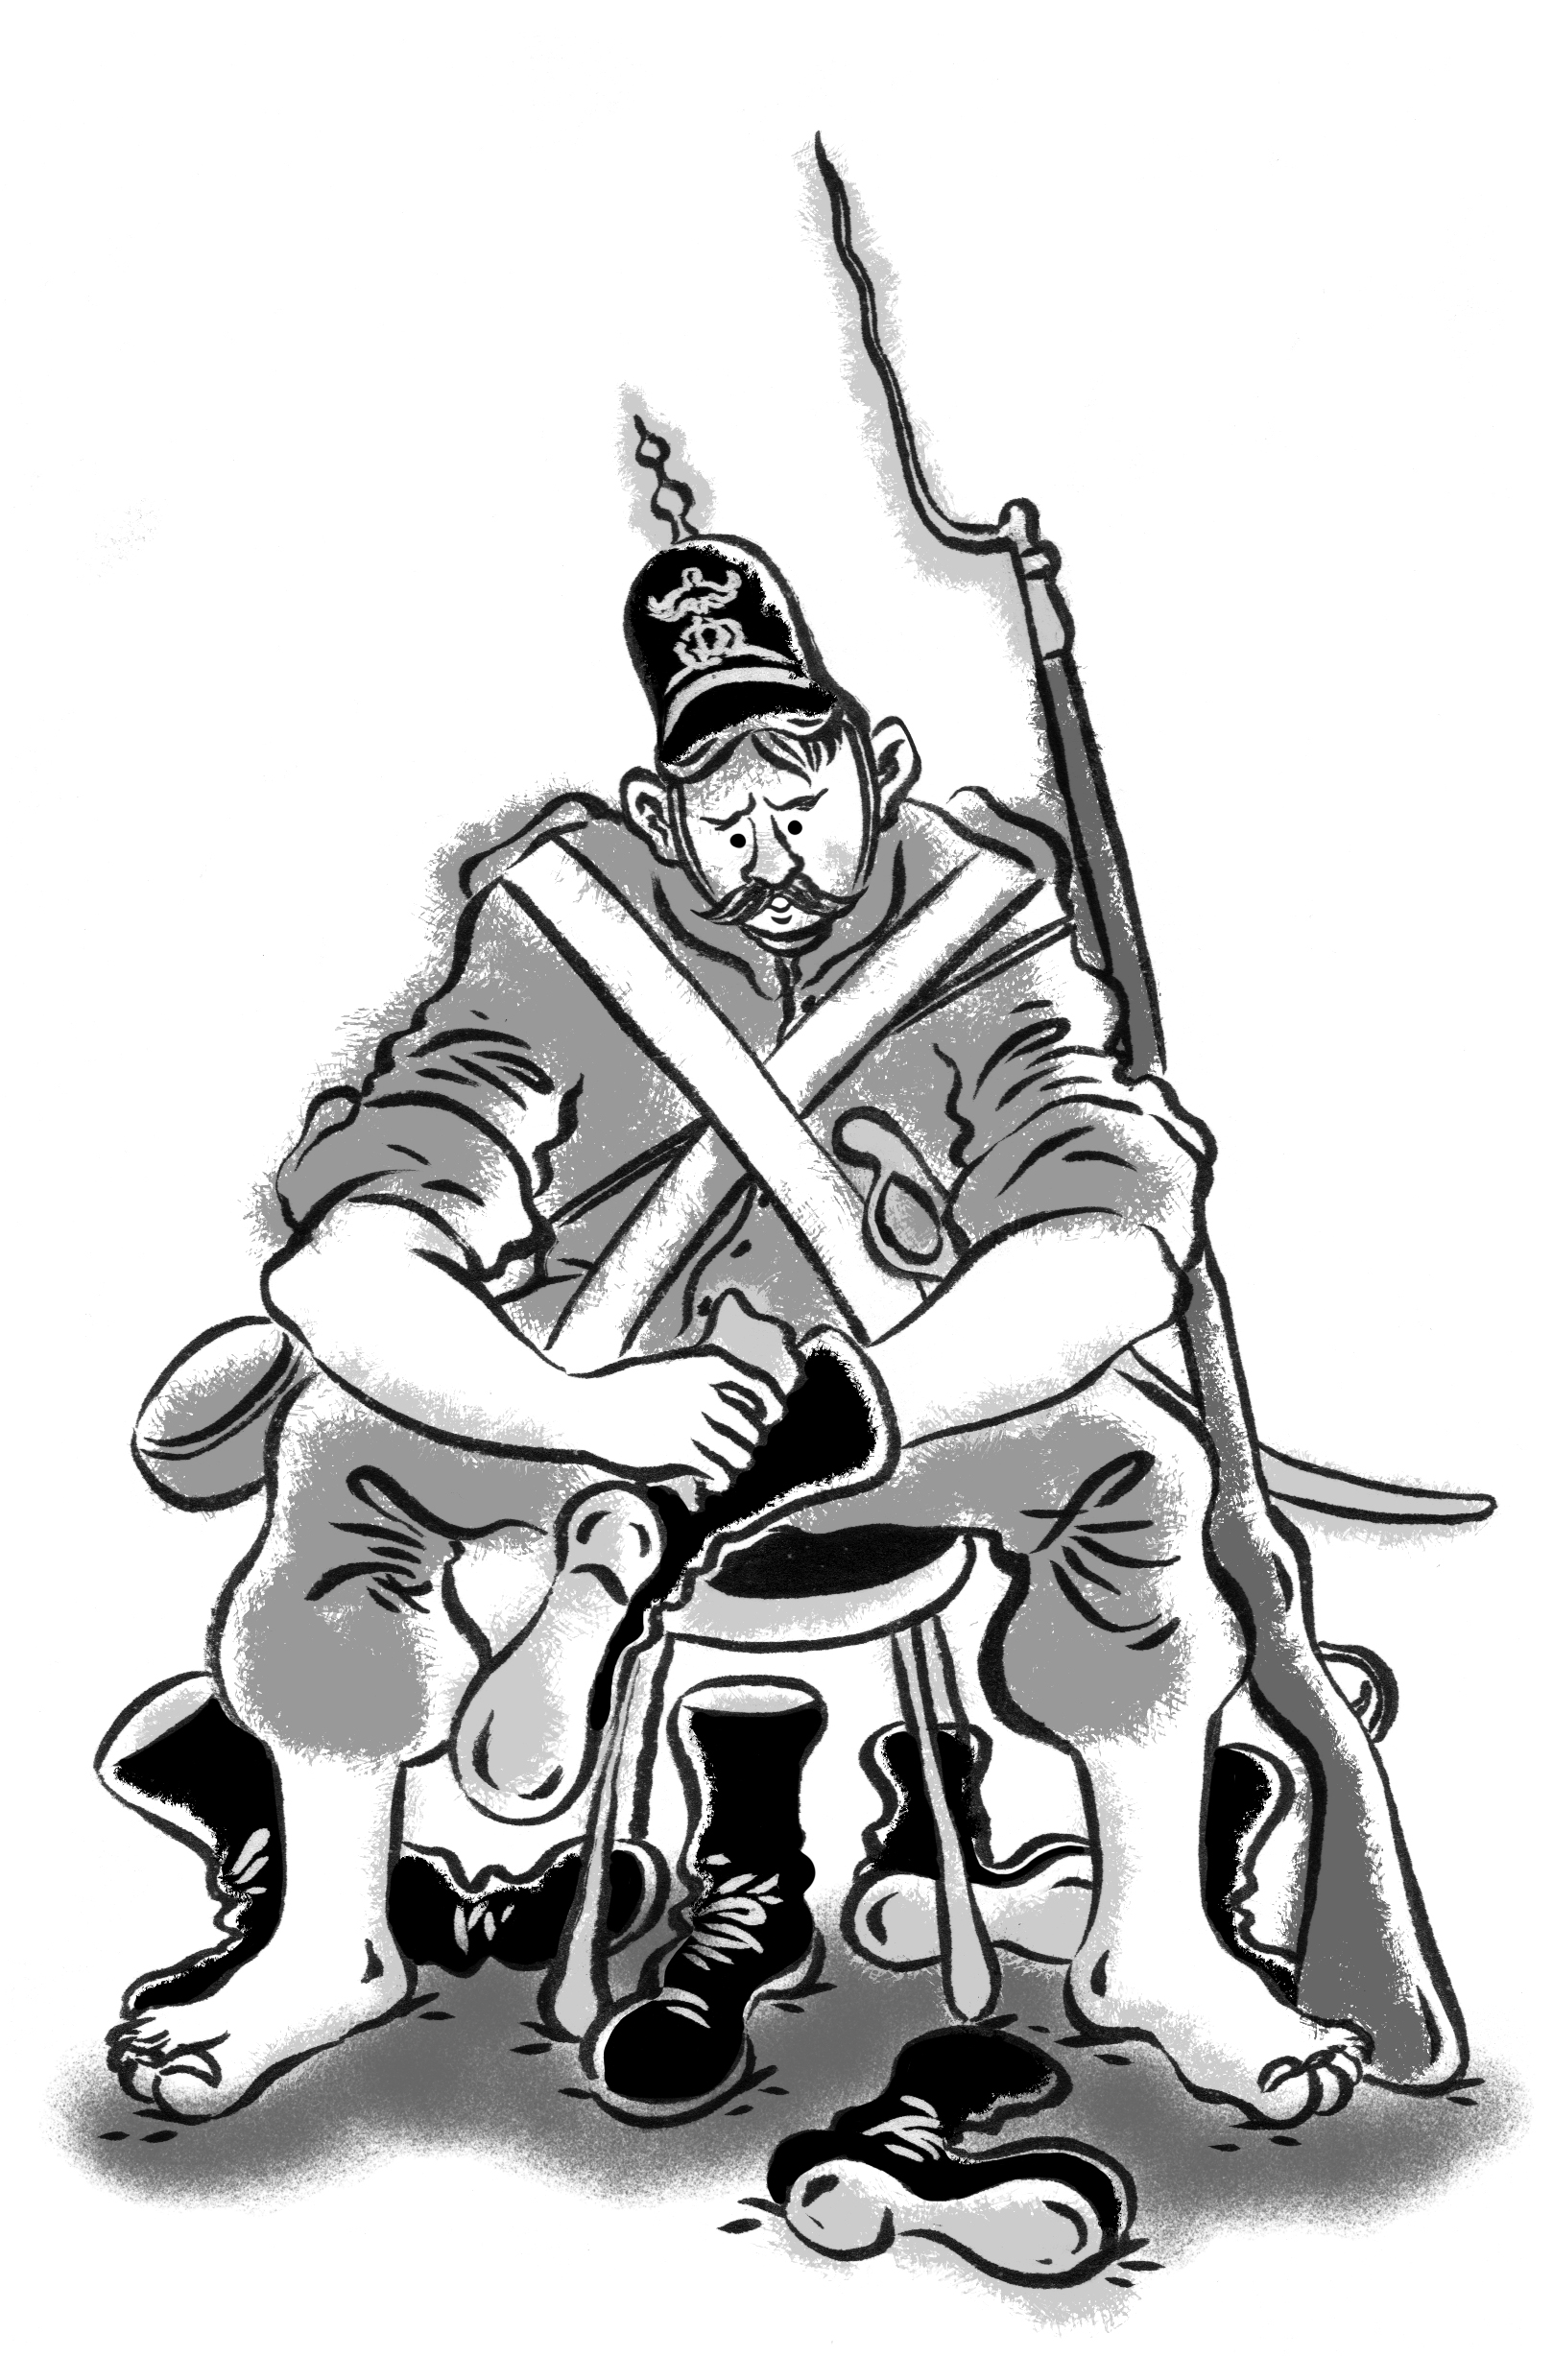
\includegraphics{./imgs/cena5.jpg}
\end{figure}

Era impossível vigiá"-lo no deserto distante e selvagem, ele reprimia a
seu bel"-prazer. Mas não era o único a se portar assim, havia outros
arbitrários e um deles era o ladrão audaz de nome Khabibula. Ele começou
a roubar os melhores cavalos do Cã Djangar, e por muito tempo não havia
quem pudesse capturar o velhaco. Mas, um dia, houve uma rixa entre os
tártaros e Khabibula foi ferido e aprisionado. Isso aconteceu num
momento em que Cã Djangar tinha pressa de ir a Penza e não conseguiria
acampar e julgar Khabibula, punindo"-o com uma execução tão terrível, que
produziria medo e terror nos outros ladrões.

Para não chegar atrasado à feira de Penza e não aparecer com Khabibula
onde houvesse autoridades russas, Cã Djangar resolveu deixar, perto de
uma fonte pequena e exígua, Panka com um cavalo e o prisioneiro ferido
acorrentado nele. O cã deu painço e um odre de água e ordenou
severamente a Panka:

--- Guarde esse homem como a sua alma! Entendeu?

Panka disse:

--- Como não entender? Entendi perfeitamente e vou fazer exatamente o
que disse.

Cã Djangar partiu com sua horda, e Panka deu de dizer a Khabibula:

--- Veja até onde a sua roubalheira o levou! Você é muito valente, só
que toda a sua valentia não foi usada para o bem, mas para o mal. Seria
melhor você se emendar.

E Khabibula respondeu:

--- Se não me emendei até agora, é tarde demais.

--- Como ``tarde demais''? A questão toda é a pessoa querer de verdade,
e o resto vem por si só\ldots{} Afinal, você tem uma alma como todo mundo:
abandone o mal, e Deus conceberá uma forma de ajudá"-lo a fazer o bem, e
tudo ficará bem.

Khabibula ouviu e suspirou.

--- Não --- disse ---, pensar nisso agora é um despropósito!

--- Mas por que um despropósito?

--- Porque estou acorrentado, à espera da morte.

--- Então eu o liberto.

Khabibula não acreditava nos próprios ouvidos, mas Panka sorriu, afável,
e disse:

--- Não estou brincando, estou dizendo a verdade. Cã me disse para
guardá"-lo ``como a própria alma'', e você sabe como se deve guardar uma
alma? Meu velho, não se tem piedade dela, é ela que sofre pelo próximo.
E agora é disto que preciso, pois não posso suportar quando os outros
padecem --- vou tirar suas algemas e colocá"-lo em um cavalo. Vá para
onde quiser, salve"-se, e, se voltar a cometer o mal, não será a mim que
enganará, mas ao Senhor.

Dizendo isso, agachou"-se, quebrou as correntes de ferro de Khabibula,
montou"-o em um cavalo e disse:

--- Saia pelo mundo, aos quatro ventos.

E Panka ficou ali aguardando o regresso de Cã Djangar e o aguardou por
muito tempo, até o riacho secar e quase não restar água no odre.

Então veio Cã Djangar acompanhado por seu séquito.

Ele olhou e perguntou:

--- Mas onde está Khabibula?

Panka respondeu:

--- Soltei"-o.

--- Como soltou? O que está me dizendo?

--- Estou lhe dizendo que segui verdadeiramente a sua ordem e o seu
desejo. Você me mandou guardar Khabibula como a minha alma, e a minha
alma eu guardo livrando"-a da necessidade de se atormentar pelo
próximo\ldots{} Pois você queria torturar Khabibula, e eu não suporto quando
torturam um homem; pegue"-me e mande que me torturem no lugar dele, para
que minha alma seja feliz e livre de todos os medos, porque não tenho
nem uma gota de medo de você nem dos outros homens, não tenho medo de
ninguém.

Cã Djangar lançou os olhos para todas as direções, depois ajeitou
o solidéu na cabeça e disse a seus homens:

--- Cheguem mais perto: vou dizer o que penso.

Os tártaros se apertaram em volta do cã. E ele disse baixinho:

--- Ao que parece, não podemos executar Panka, pode ser que exista um
anjo dentro dele\ldots{}

--- Sim --- responderam os tártaros, todos em voz baixa ---, não podemos
fazer mal a ele: não o compreendemos por muitos anos, mas agora, em um
instante, tudo ficou claro; pode ser que ele seja um justo.

\medskip

{\footnotesize\hfill\emph{Tradução: Irineu Franco Perpetuo.}}




\chapter*{}
\label{part6}
\thispagestyle{empty}

\begin{vplace}[1.5]
{\HUGES\hfill\textbl{АNTON TCHÉKHOV}}

{\LARGE\hfill\textlt(1860–1904)}
\end{vplace}

\pagebreak
\thispagestyle{empty}
\mbox{}
\vfill
\begin{center}
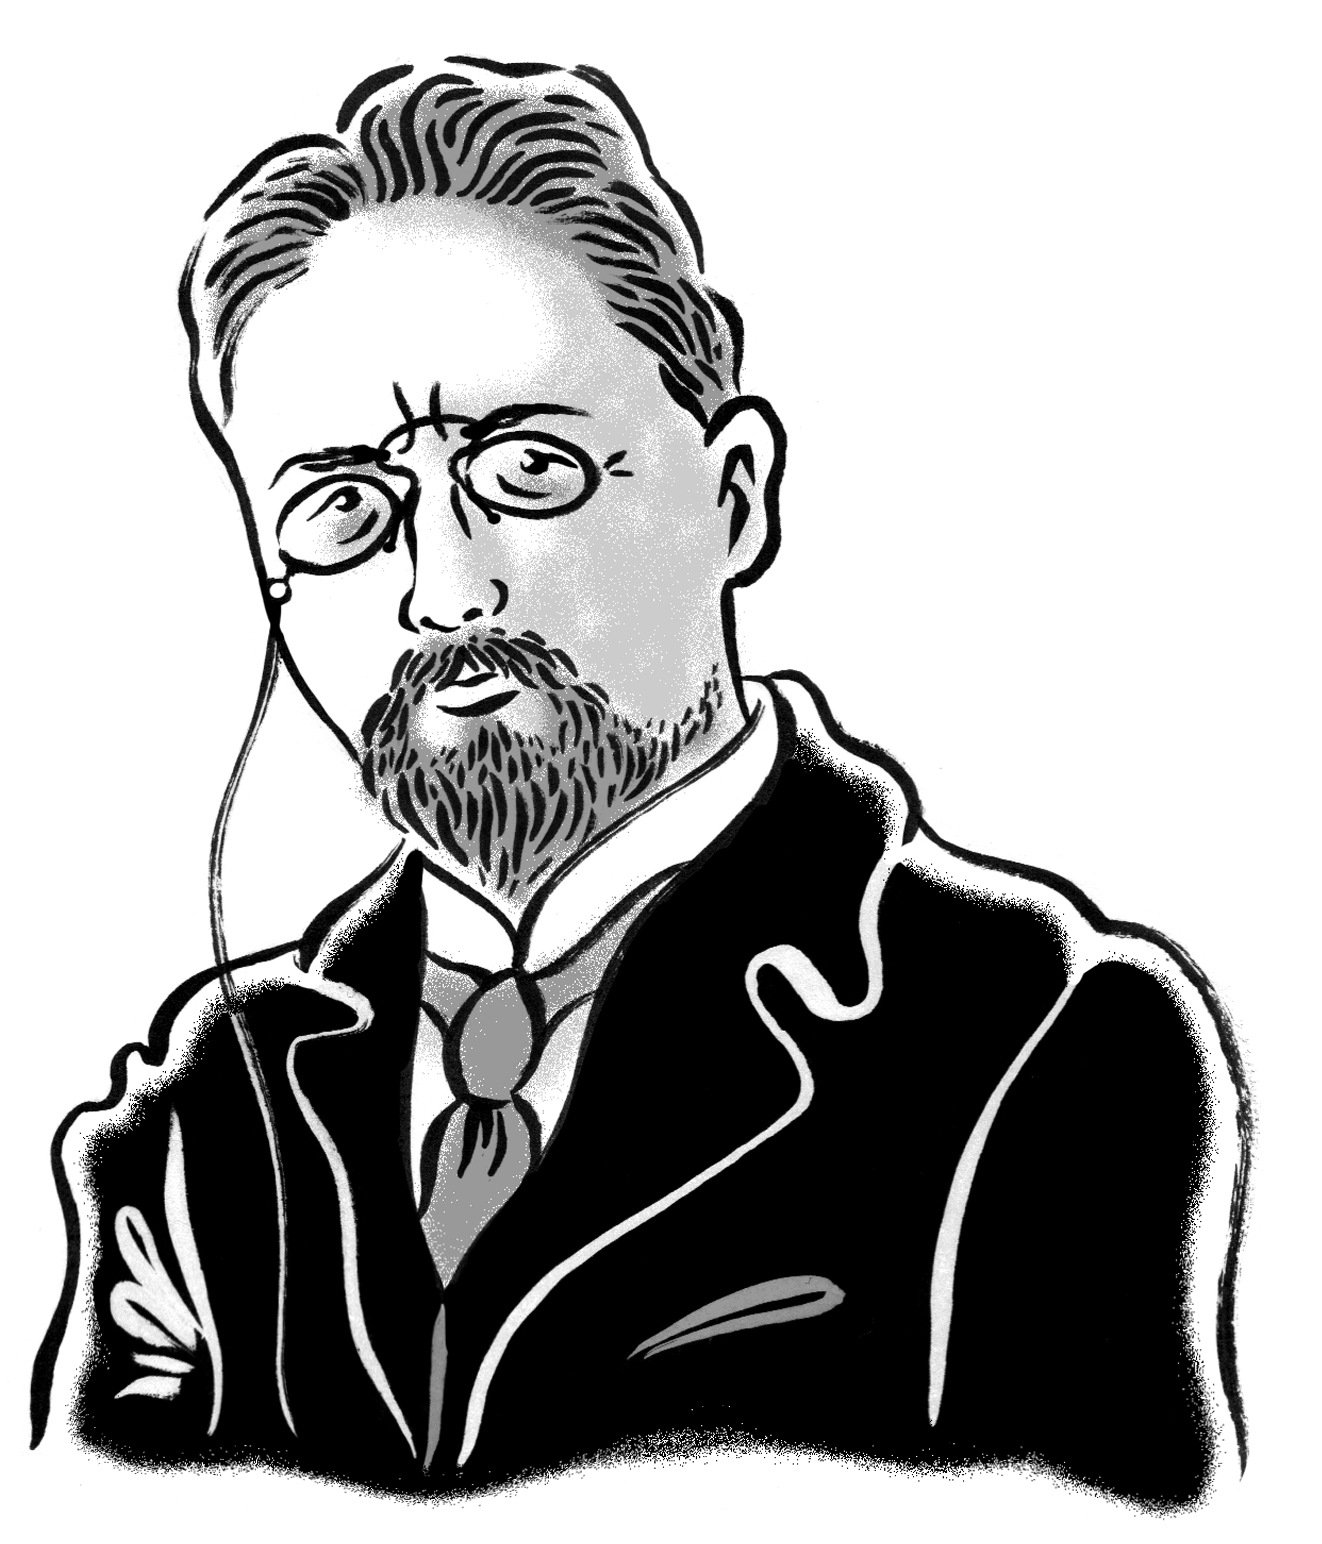
\includegraphics[width=6cm]{./imgs/autor6.jpg}
\end{center}

\chapter{Vanka}

Vanka Júkov, menino de nove anos que fora levado, três meses antes, à
casa do sapateiro Aliákhin para aprender o ofício, não foi para a cama
na noite de Natal. Após o patrão e os aprendizes saírem para as matinas,
o menino pegou no armário do patrão um frasquinho de tinta e uma caneta
de pena enferrujada e, abrindo uma folha de papel amarrotada, começou a
escrever. Antes de desenhar a primeira letra, lançou alguns olhares para
a porta e as janelas, espiando o ícone escurecido, nas quais se
estendiam dos dois lados prateleiras para sapatos, e suspirou
entrecortado. O papel estava em um banco diante do qual ele se
ajoelhara.

``Querido vovô Konstantin Makárytch!'', escreveu ele. ``Estou lhe
escrevendo uma carta. Desejo que tenha um feliz Natal e que Deus lhe dê
tudo de bom. Não tenho pai nem mãe, só me sobrou você.''

Vanka virou os olhos para a janela escura, onde tremeluzia o reflexo de
sua vela, imaginando vivamente seu avô, Konstantin Makárytch, que
trabalhava de guarda noturno na casa dos senhores Jívarev. Era um
velhote magricela de 65 anos, mas extraordinariamente ágil e vivaz, de
rosto sempre sorridente e olhos ébrios. De dia, dormia na cozinha dos
serviçais ou gracejava com as cozinheiras; já à noite, agasalhado com um
sobretudo de peles, andava em torno da propriedade e girava sua matraca.
Atrás dele, de cabeça baixa, iam a velha cadela Castanha e o cãozinho
Enguia, que recebera esse nome devido à cor negra e ao corpo comprido de
doninha. O Enguia era muito respeitoso e amável, olhava com o mesmo
afeto para pessoas de casa e para estranhos, mas não era digno de
confiança. Debaixo de seu respeito e submissão, ocultava"-se uma malícia
jesuítica. Ninguém melhor do que ele sabia a hora de chegar
sorrateiramente e morder a perna de alguém, meter"-se na cave fria de
mantimentos, ou roubar a galinha de um mujique. Mais de uma vez apanhara
nas patas traseiras, chegara a ser pendurado duas vezes, levava surras
semanais até ficar semimorto, mas sempre sobrevivia.

Agora, provavelmente, o avô estava no portão apertando os olhos para ver
o vermelho intenso saindo das janelas iluminadas da igreja da aldeia
e, batendo no chão com as botas de feltro, gracejava com a criadagem.
Sua matraca ficava amarrada ao cinto. Esfregava as mãos, encolhia"-se de
frio e, com risinho de velho, beliscava ora a copeira, ora a cozinheira.

--- Não quer cheirar rapé? --- dizia oferecendo a tabaqueira às
mulheres.

As mulheres cheiravam e espirravam. Vovô entrava em um êxtase
indescritível, dava uma risada alegre e gritava:

--- Arranquem do nariz, o tabaco congelou!

Também esticava o tabaco para os cachorros cheirarem. Castanha
espirrava, revirava o focinho e, ofendida, afastava"-se para o lado. Já
Enguia, por respeito, não espirrava e abanava a cauda. O tempo estava
magnífico. O ar calmo, transparente e fresco. A noite era escura, mas se
podia ver toda a aldeia com seus telhados brancos, os fios de fumaça
saindo das chaminés, as árvores prateadas pela geada, os montes de neve.
O céu se cobria de estrelas cintilantes, e a Via Láctea delineava"-se tão
clara, que era como se tivesse sido lavada e polida com neve antes das
festas\ldots{}

Vanka suspirou, molhou a pena e continuou a escrever:

``Ontem eu levei um castigo. O patrão me arrastou pelos cabelos no
quintal e me bateu com a cinta, porque eu estava embalando o bebezinho
deles no berço e, por acidente, peguei no sono. Durante a semana, a
patroa me mandou limpar um arenque, eu comecei pelo rabo e ela pegou o
peixe e meteu o focinho dele na minha cara. Os aprendizes riem de mim,
mandam"-me buscar vodca na taberna e roubar pepinos do sapateiro, que
bate com o que lhe cair na mão. E ganho um nada de comida. De manhã dão
pão, no almoço mingau e, de noite, pão de novo; o chá e a sopa de
repolho, os patrões os dividem entre si. Mandam"-me dormir no corredor da
entrada e, quando o bebezinho chora, eu não prego o olho e fico
balançando o berço. Querido vovô, faça uma graça divina, leve"-me embora
para casa, para a aldeia, não tenho chance aqui\ldots{} Juro de joelhos que
vou sempre orar a Deus, leve"-me daqui, senão eu morro\ldots{}''.

Vanka entortou a boca, enxugou os olhos com o punho preto e soluçou.

``Vou picar tabaco para você'', prosseguiu ele, ``orar a Deus e, se for
preciso, açoite"-me sem piedade. Se você achar que não terei serventia,
pedirei ao administrador que me deixe, pelo amor de Deus, limpar botas
ou tomar o lugar de Fédia de ajudante de pastor. Querido vovô, aqui não
tenho chance nenhuma, apenas a morte. Queria fugir a pé para a aldeia,
mas não tenho botas e tenho medo do frio. E, quando eu ficar grande, vou
alimentá"-lo, não deixarei ninguém ofendê"-lo e, depois que você morrer,
rezarei por sua alma, como pela alma da mamãe Pelagueia.

Moscou é uma cidade grande. As casas são todas senhoriais e há uma
porção de cavalos, mas não tem ovelhas, e os cachorros não são bravos.
Os meninos não andam com estrelas,\footnote{Meninos do coro, como um
  ritual natalino, tinham o costume de andar segurando estrelas.
  Acompanhados pelo diácono, iam de casa em casa e, onde tivessem
  permissão de entrar, cantavam diante do ícone.} e ali não deixam
ninguém cantar no coro da igreja; uma vez eu vi, pela janela de uma
loja, venderem anzóis com linha, para qualquer tipo de peixe, os olhos
da cara, e existe até anzol que aguenta um bagre de mais de quinze
quilos. E vi cada loja, com espingardas de fidalgo que não devem
sair por menos de cem rublos \ldots{} E os açougues têm tetrazes, perdizes e
lebres, mas lá os vendedores não dizem onde foram abatidos.

Querido vovô, quando o patrão armar a árvore de Natal com guloseimas,
pegue uma noz dourada para mim e esconda no bauzinho verde. Peça à
senhorita Olga Ignátivena, diga que é para Vanka.''

Vanka suspirou convulsivamente e voltou a fitar a janela. Lembrava que o
avô sempre ia buscar uma árvore de Natal na floresta para os patrões e o
levava consigo. Que tempo feliz! Vovô grasnava, o gelo grasnava e, ao
olhar para eles, Vanka grasnava. Antes de podar a árvore, o avô fumava
cachimbo, tragando o tabaco longamente e rindo do pequeno Vanka
congelado\ldots{} Os novos abetos, cobertos de geada, ficavam imóveis,
esperando para saber qual deles morreria. Não se sabe de onde, uma lebre
vinha voando pelos montes de neve\ldots{} O avô não se continha e começava a
gritar:

--- Segure, segure\ldots{} segure! Ah, diabo de rabo cortado!

O avô arrastava o abeto cortado até a casa senhorial, onde se punham a
enfeitá"-lo\ldots{} A mais empenhada era a senhorita Olga Ignátievna, a
favorita de Vanka. Quando a mãe de Vanka, Pelagueia, ainda era viva e
trabalhava como arrumadeira dos patrões, Olga Ignátievna dava balas ao
menino e, por falta do que fazer, ensinou"-o a ler, a escrever, a contar
até cem e até a dançar quadrilha. Quando Pelagueia morreu, mandaram o
órfão para o avô, na cozinha dos serviçais, e da cozinha para Moscou,
para o sapateiro Aliákhin\ldots{}

``Venha, vovô querido'', continuava Vanka, ``imploro ao Senhor Jesus
Cristo, leve"-me daqui. Tenha piedade de mim, um órfão infeliz que apanha
sem parar e quer desesperadamente comer; e é tamanha tristeza, que nem
se pode explicar, choro o tempo todo. Outro dia o patrão me golpeou na
cabeça com uma forma de sapato de tal jeito, que eu caí e com muito
custo recobrei os sentidos. Minha vida está perdida, sou pior do que um
cachorro\ldots{} Lembranças para Aliona, o zarolho Egorka e o cocheiro, e não
dê meu acordeão a ninguém. Sempre seu neto, Ivan\footnote{Vanka é
  apelido de Ivan.} Júkov, venha, vovô querido.''

Vanka dobrou em quatro a folha rabiscada, colocando"-a no envelope que
comprara na véspera por um copeque\ldots{} Após pensar um pouco, umedeceu a
pena e escreveu o endereço:

``Para a aldeia do vovô''.

Depois se coçou, pensou de novo e acrescentou: ``Konstantin Makárytch''.
Satisfeito por não ter sido impedido de escrever, colocou o gorro e saiu
correndo à rua em mangas de camisa\ldots{}

Os vendedores do açougue que ele interrogara na véspera disseram que as
cartas eram deixadas nas caixas de correio e das caixas se espalhavam
pelo mundo em troicas postais com cocheiros bêbados e sinetas sonoras.
Vanka correu à caixa de correio mais próxima e enfiou a preciosa carta
pela fresta\ldots{}

\begin{figure}[ht!]
\vspace*{-1.6cm}
\hspace*{-1.8cm}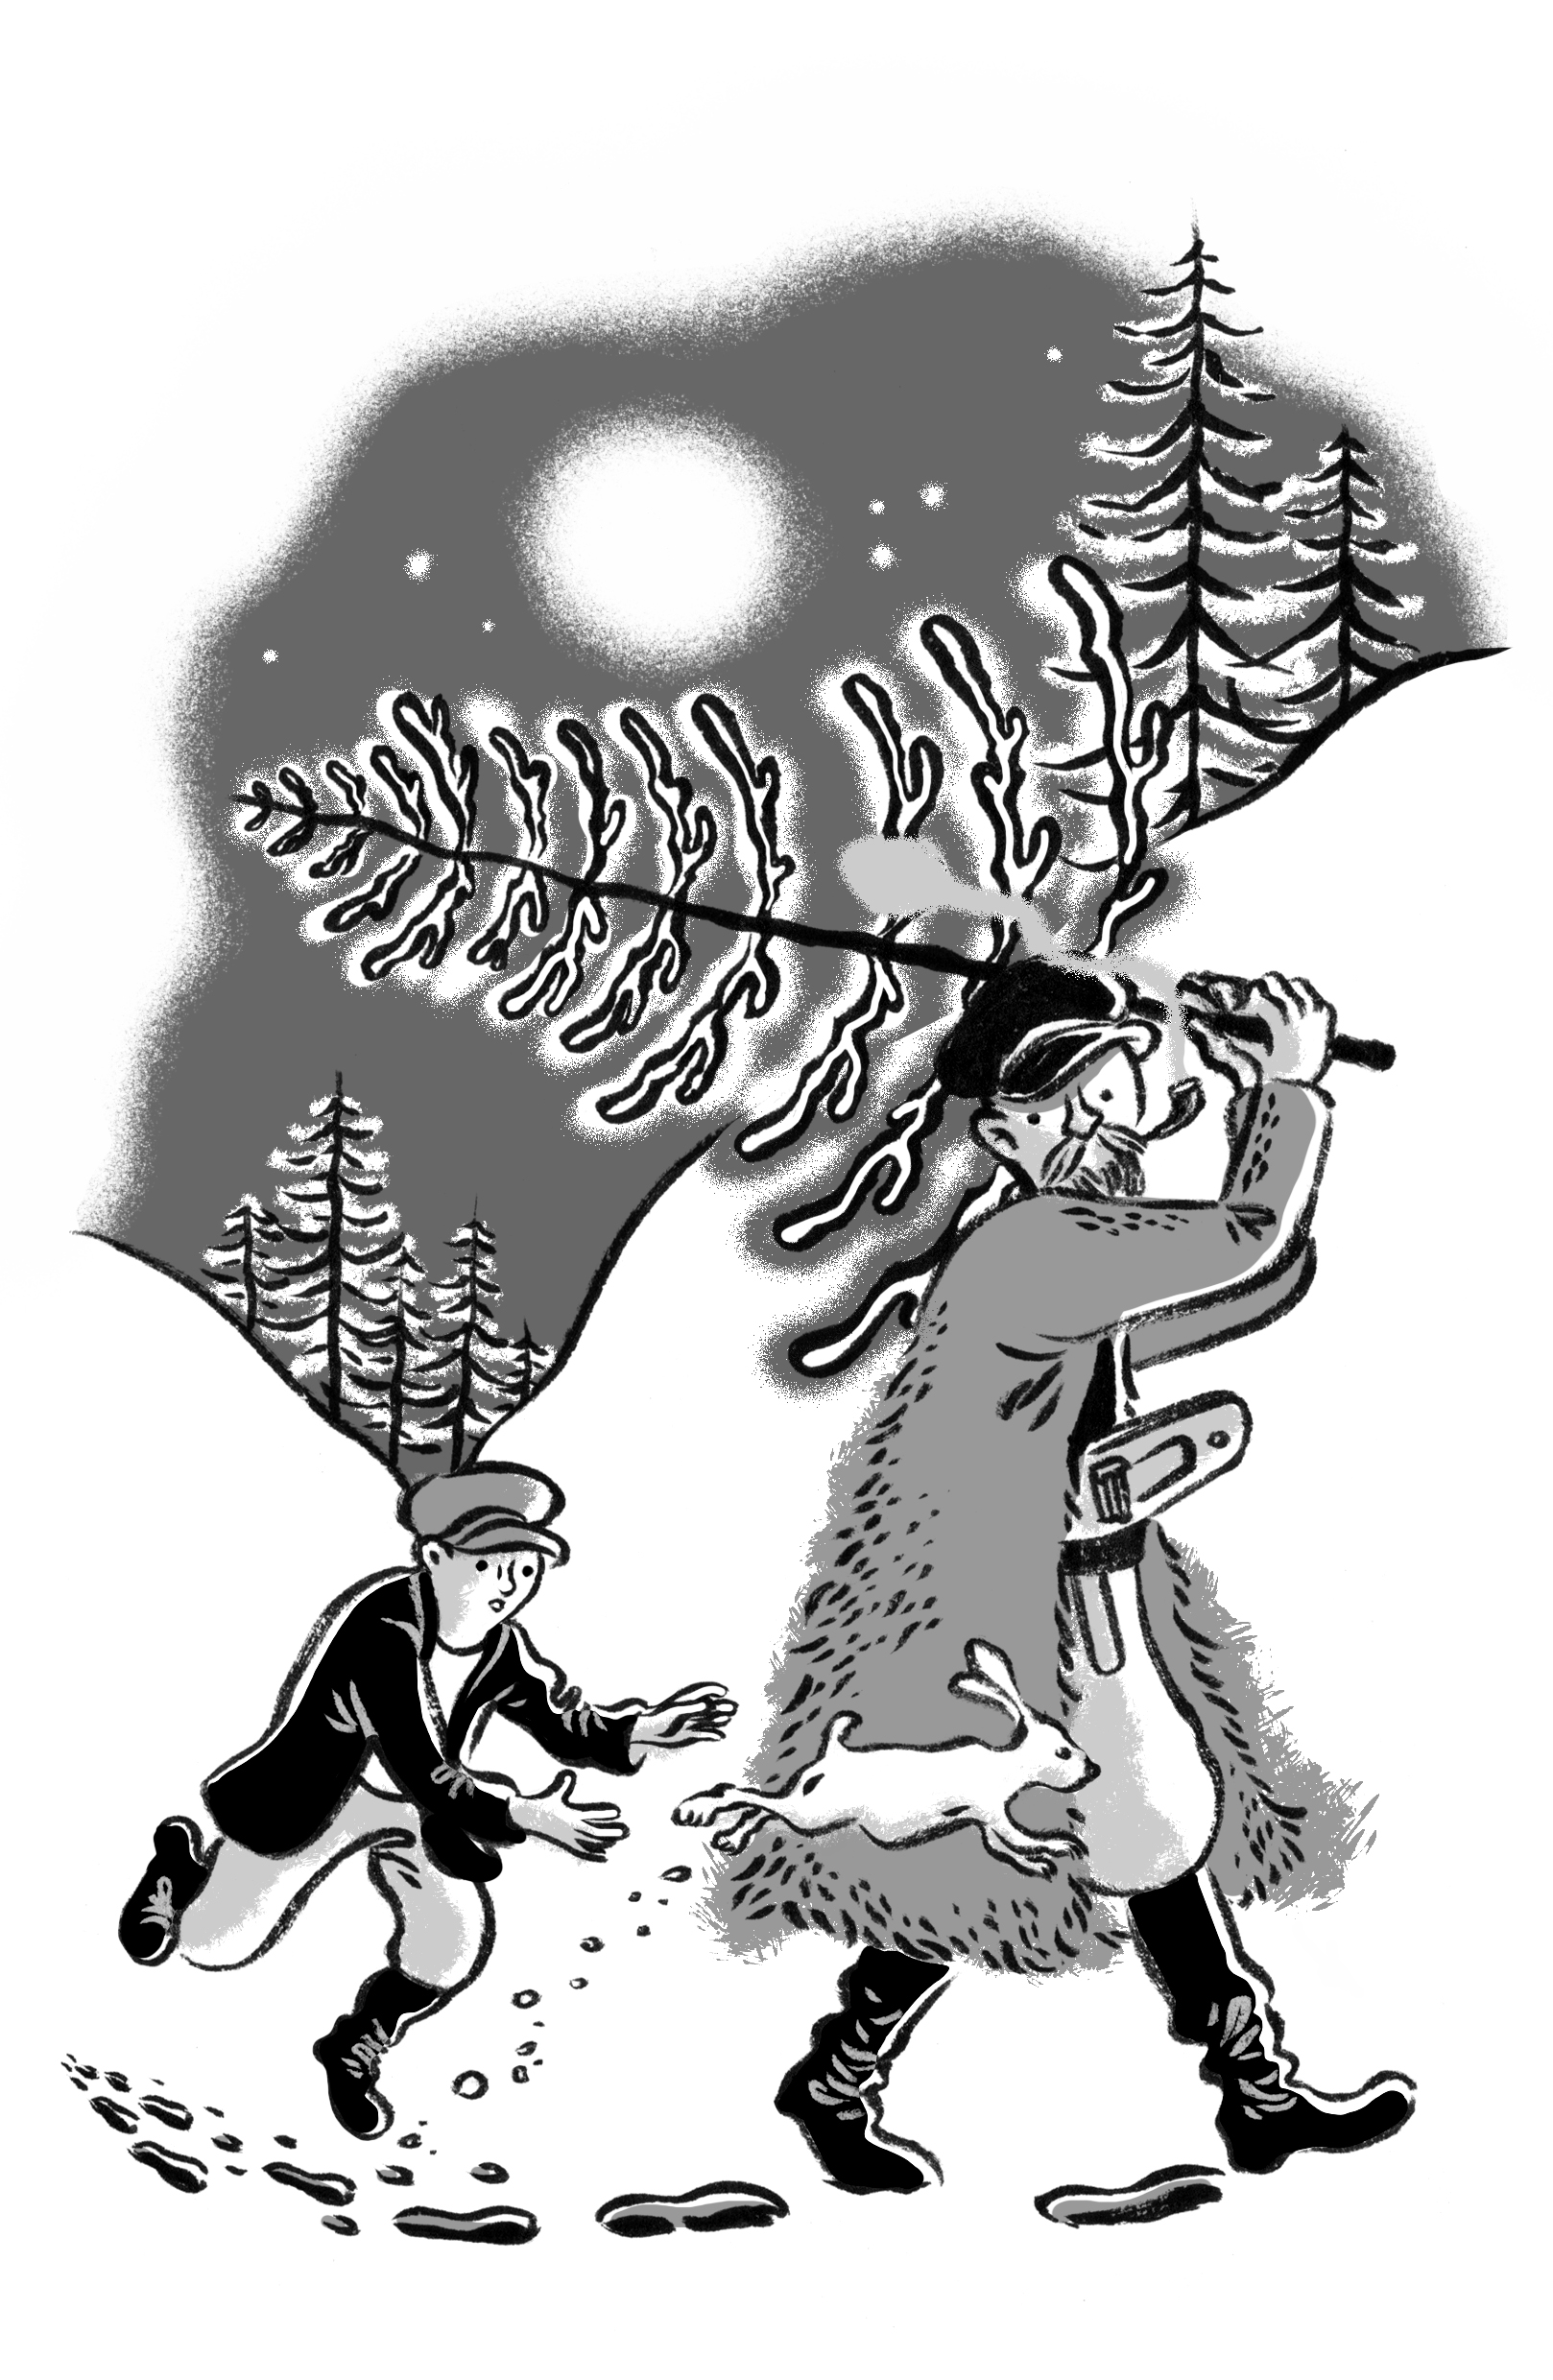
\includegraphics{./imgs/cena6.jpg}
\end{figure}

\textls[-4]{Embalado por esperanças doces, dormiu profundamente uma hora depois\ldots{}
Sonhou com uma lareira. Ao lado, estava sentado seu avô, com os pés
descalços erguidos, lendo a carta para as cozinheiras\ldots{} Enguia andava
em volta e abanava a cauda\ldots{}}

\medskip

{\footnotesize\hfill\emph{Tradução: Irineu Franco Perpetuo.}}

\chapter{O fugitivo}\label{part7}

Foi um procedimento longo. Primeiro, Pachka andou com a mãe debaixo de
chuva por um campo ceifado, em seguida por veredas do bosque, onde
folhas amarelas grudavam nas botinhas dele, e caminhou até amanhecer.
Depois, ficou duas horas num saguão escuro esperando uma porta se abrir.
No saguão não era tão frio e úmido como no pátio, mas mesmo ali o vento
jogava respingos de chuva. Quando o saguão, aos poucos, foi ficando
abarrotado de gente, Pachka, encolhido, apertou o rosto contra o
sobretudo de peles de alguém, com cheiro forte de peixe salgado, e
cochilou. Então o ferrolho rangeu, a porta se abriu, e Pachka entrou com
a mãe na sala de recepção. Lá novamente teve que esperar muito tempo.
Sentados em bancos, todos os doentes estavam imóveis e em silêncio.
Pachka olhou para eles e também ficou em silêncio, embora visse muita
coisa estranha e engraçada. Quando um rapaz entrou na recepção pulando
sobre um pé, Pachka teve vontade de pular do mesmo jeito; cutucou o
cotovelo da mãe, deu um riso em sua manga e disse:

--- Veja, mamãe: um pardal!

--- Silêncio, filho, silêncio! --- disse a mãe.

Um enfermeiro sonolento apareceu na janelinha.

--- Venham se registrar! --- disse com voz grossa.

Todos, incluindo o rapaz que pulava de jeito engraçado, arrastaram"-se à
janelinha. A todo mundo o enfermeiro perguntava o nome e o patronímico,
a idade, o local de residência, quanto tempo estava doente, etc. Pelas
respostas de sua mãe, Pachka ficou sabendo que não se chamava Pachka,
mas Pável\footnote{Pachka é apelido de Pável.} Galaktiónov, que tinha
sete anos, não era alfabetizado e estava doente desde a Páscoa.

Logo após o registro, foi preciso esperar um pouco; um médico de avental
branco e toalha na cintura percorreu a sala de recepção. Passando ao
lado do rapaz que pulava, deu de ombros e disse com voz cantante de
tenor:

--- Mas que bobo! Que foi, não é um bobo? Mandei vir na segunda"-feira, e
você veio na sexta. Para mim tanto faz se você deixar completamente de
andar, mas veja que bobo, perderá a perna!

O rapaz fez uma cara lastimosa, como se pedisse misericórdia, pestanejou
e disse:

--- Tenha piedade, Ivan Mikoláitch!

--- Não venha com ``Ivan Mikoláitch''! --- arremedou o médico. --- Disse
para vir na segunda"-feira, então tem que obedecer. Um bobo, e é tudo\ldots{}

Começou o atendimento. O médico entrou em seu quartinho e chamava os
pacientes pela ordem. De vez em quando, ouviam"-se do quarto gritos
estridentes, choro de criança ou brados zangados do médico:

--- Ora, por que está gritando? Por acaso estou lhe cortando? Pare
quieto!

Chegou a vez de Pachka.

--- Pável Galaktiónov! --- gritou o médico.

A mãe ficou aturdida, como se não esperasse o chamado, e, pegando Pachka
pela mão, levou"-o ao quartinho. O médico estava sentado à mesa, batendo
maquinalmente em um livro grosso com um martelinho.

--- O que dói? --- perguntou sem olhar para os recém"-chegados.

--- O rapazinho tem um machucado
no cotovelo, doutor --- respondeu a mãe, e seu rosto assumiu tal
expressão, que era como se de fato estivesse terrivelmente aflita pelo
machucado de Pachka.

--- Dispa"-o!

Pachka, bufando, desenrolou o lenço do pescoço, depois enxugou o nariz
na manga e se pôs a tirar o sobretudo de pele de carneiro, sem pressa.

--- Dona, isso não é uma visita social! --- disse o médico, zangado. ---
Por que essa moleza? Você não é a única que tenho que atender.

Pachka jogou apressadamente o sobretudo de pele no chão e, com ajuda da
mãe, tirou a camisa\ldots{} O médico fitou"-o com preguiça e deu tapinhas em
seu ventre nu.

--- Pachka, amiguinho, você criou uma pança respeitável --- disse ele e
suspirou. --- Pois bem, mostre o cotovelo.

O menino olhou de esguelha para uma bacia com água suja de sangue, fitou o
avental do médico e começou a chorar.

--- Buá! --- arremedou o médico. --- O travesso já está na época de
casar e fica choramingando! Vergonha.

Tentando não chorar, Pachka fitou a mãe com um pedido impresso no olhar:
``Não vá contar em casa que eu chorei no hospital!''.

O médico examinou"-lhe o cotovelo, apalpou, suspirou, seus lábios
produziram um som de reprovação, e apalpou de novo.

--- Devia levar um sopapo, dona, só não há quem bata --- disse. --- Por
que não o trouxe antes? Esse braço está perdido! Olhe aqui, mulher tola,
a junta está ferida!

--- O doutor é quem sabe\ldots{} --- suspirou a mulher.

--- O doutor\ldots{} Deixou o braço do rapaz apodrecer e agora vem dizer ``o
doutor é quem sabe''. Que trabalhador ele sairá sem um braço? Você terá
que cuidar dele para o resto da vida. Se aparecesse uma espinha no seu
nariz, você viria correndo ao hospital na mesma hora, mas deixou o
menino apodrecendo por meio ano. Vocês são todos iguais.

O homem acendeu um cigarro com boquilha de papel. Enquanto o
cigarro fumegava, ele passava uma descompostura na mulher e balançava a
cabeça no compasso de uma canção que cantarolava mentalmente, pensando
em algo alheio. Pachka estava em pé na sua frente, sem
roupa, ouvindo"-o e olhando para a fumaça. Quando o cigarro apagou, o
médico sacudiu o corpo e se pôs a falar em um tom mais grave:

--- Pois ouça, dona. Unguentos e óleos aqui não vão ajudar. Tem que
deixá"-lo no hospital.

--- Se é preciso, doutor, por que não deixá"-lo?

--- Vamos operá"-lo. Você, Pachka, ficará aqui --- disse o médico,
batendo no ombro do menino. --- Sua mãe irá embora, mas nós ficaremos
aqui, amiguinho. Aqui é bom, uma beleza! Vamos nos ajeitar bem, Pachka,
iremos apanhar pintassilgos e eu lhe mostrarei uma raposa! Faremos
visitas juntos! Hem? Quer? E mamãe amanhã virá vê"-lo! Hem?

Pachka fitou a mãe de forma interrogativa.

--- Fique, filho! --- disse ela.

--- Fique, fique! --- gritou o médico, alegre. --- Não há o que
discutir! Vou lhe mostrar uma raposa viva! Iremos juntos à feira comprar
balas! Mária Deníssovna, leve"-o para cima!

O médico, pelo visto um sujeito alegre e bondoso, estava alegre com a
companhia; Pachka quis satisfazê"-lo, principalmente porque nunca na vida
tinha estado na feira e veria uma raposa viva de bom grado, mas como se
viraria sem a mãe? Depois de ponderar um pouco, resolveu pedir ao doutor
que deixasse sua mãe também ficar no hospital, mas, nem bem abriu a
boca, a enfermeira o levou escada acima. Ele foi olhando para os lados,
boquiaberto. A escada, o chão e o umbral --- enormes, lisos e brilhantes
--- estavam pintados de um magnífico amarelo, exalando um odor delicioso
de tinta a óleo. Por todo lado havia lâmpadas, passadeiras se estendiam,
torneiras de cobre ressaltavam nas paredes. E mais do que tudo Pachka
gostou da cama em que o acomodaram e do cobertor cinza e áspero. Apalpou
o travesseiro e o cobertor, deu uma olhada na enfermaria e decidiu que
se vivia muito bem com o médico.

A enfermaria dele não era grande, consistia apenas em três leitos. Um
leito estava vazio, o outro era ocupado por Pachka, e o terceiro por um
velho de olhos azedos que tossia e cuspia em uma caneca o tempo inteiro.
Da cama de Pachka, avistava"-se, pela porta, uma parte de outra
enfermaria, com dois leitos: em um dormia um homem muito pálido e
descarnado, com um saco de borracha na cabeça; no outro, apoiando"-se nos
braços abertos, estava sentado um mujique de cabeça enfaixada que
lembrava muito uma mulher.

A enfermeira, após acomodar Pachka, saiu e, pouco depois, voltou
trazendo uma pilha de roupas.

--- É para você --- disse. --- Vista"-se.

\begin{figure}%[ht!]
\vspace*{-2.2cm}
\hspace*{-2.5cm}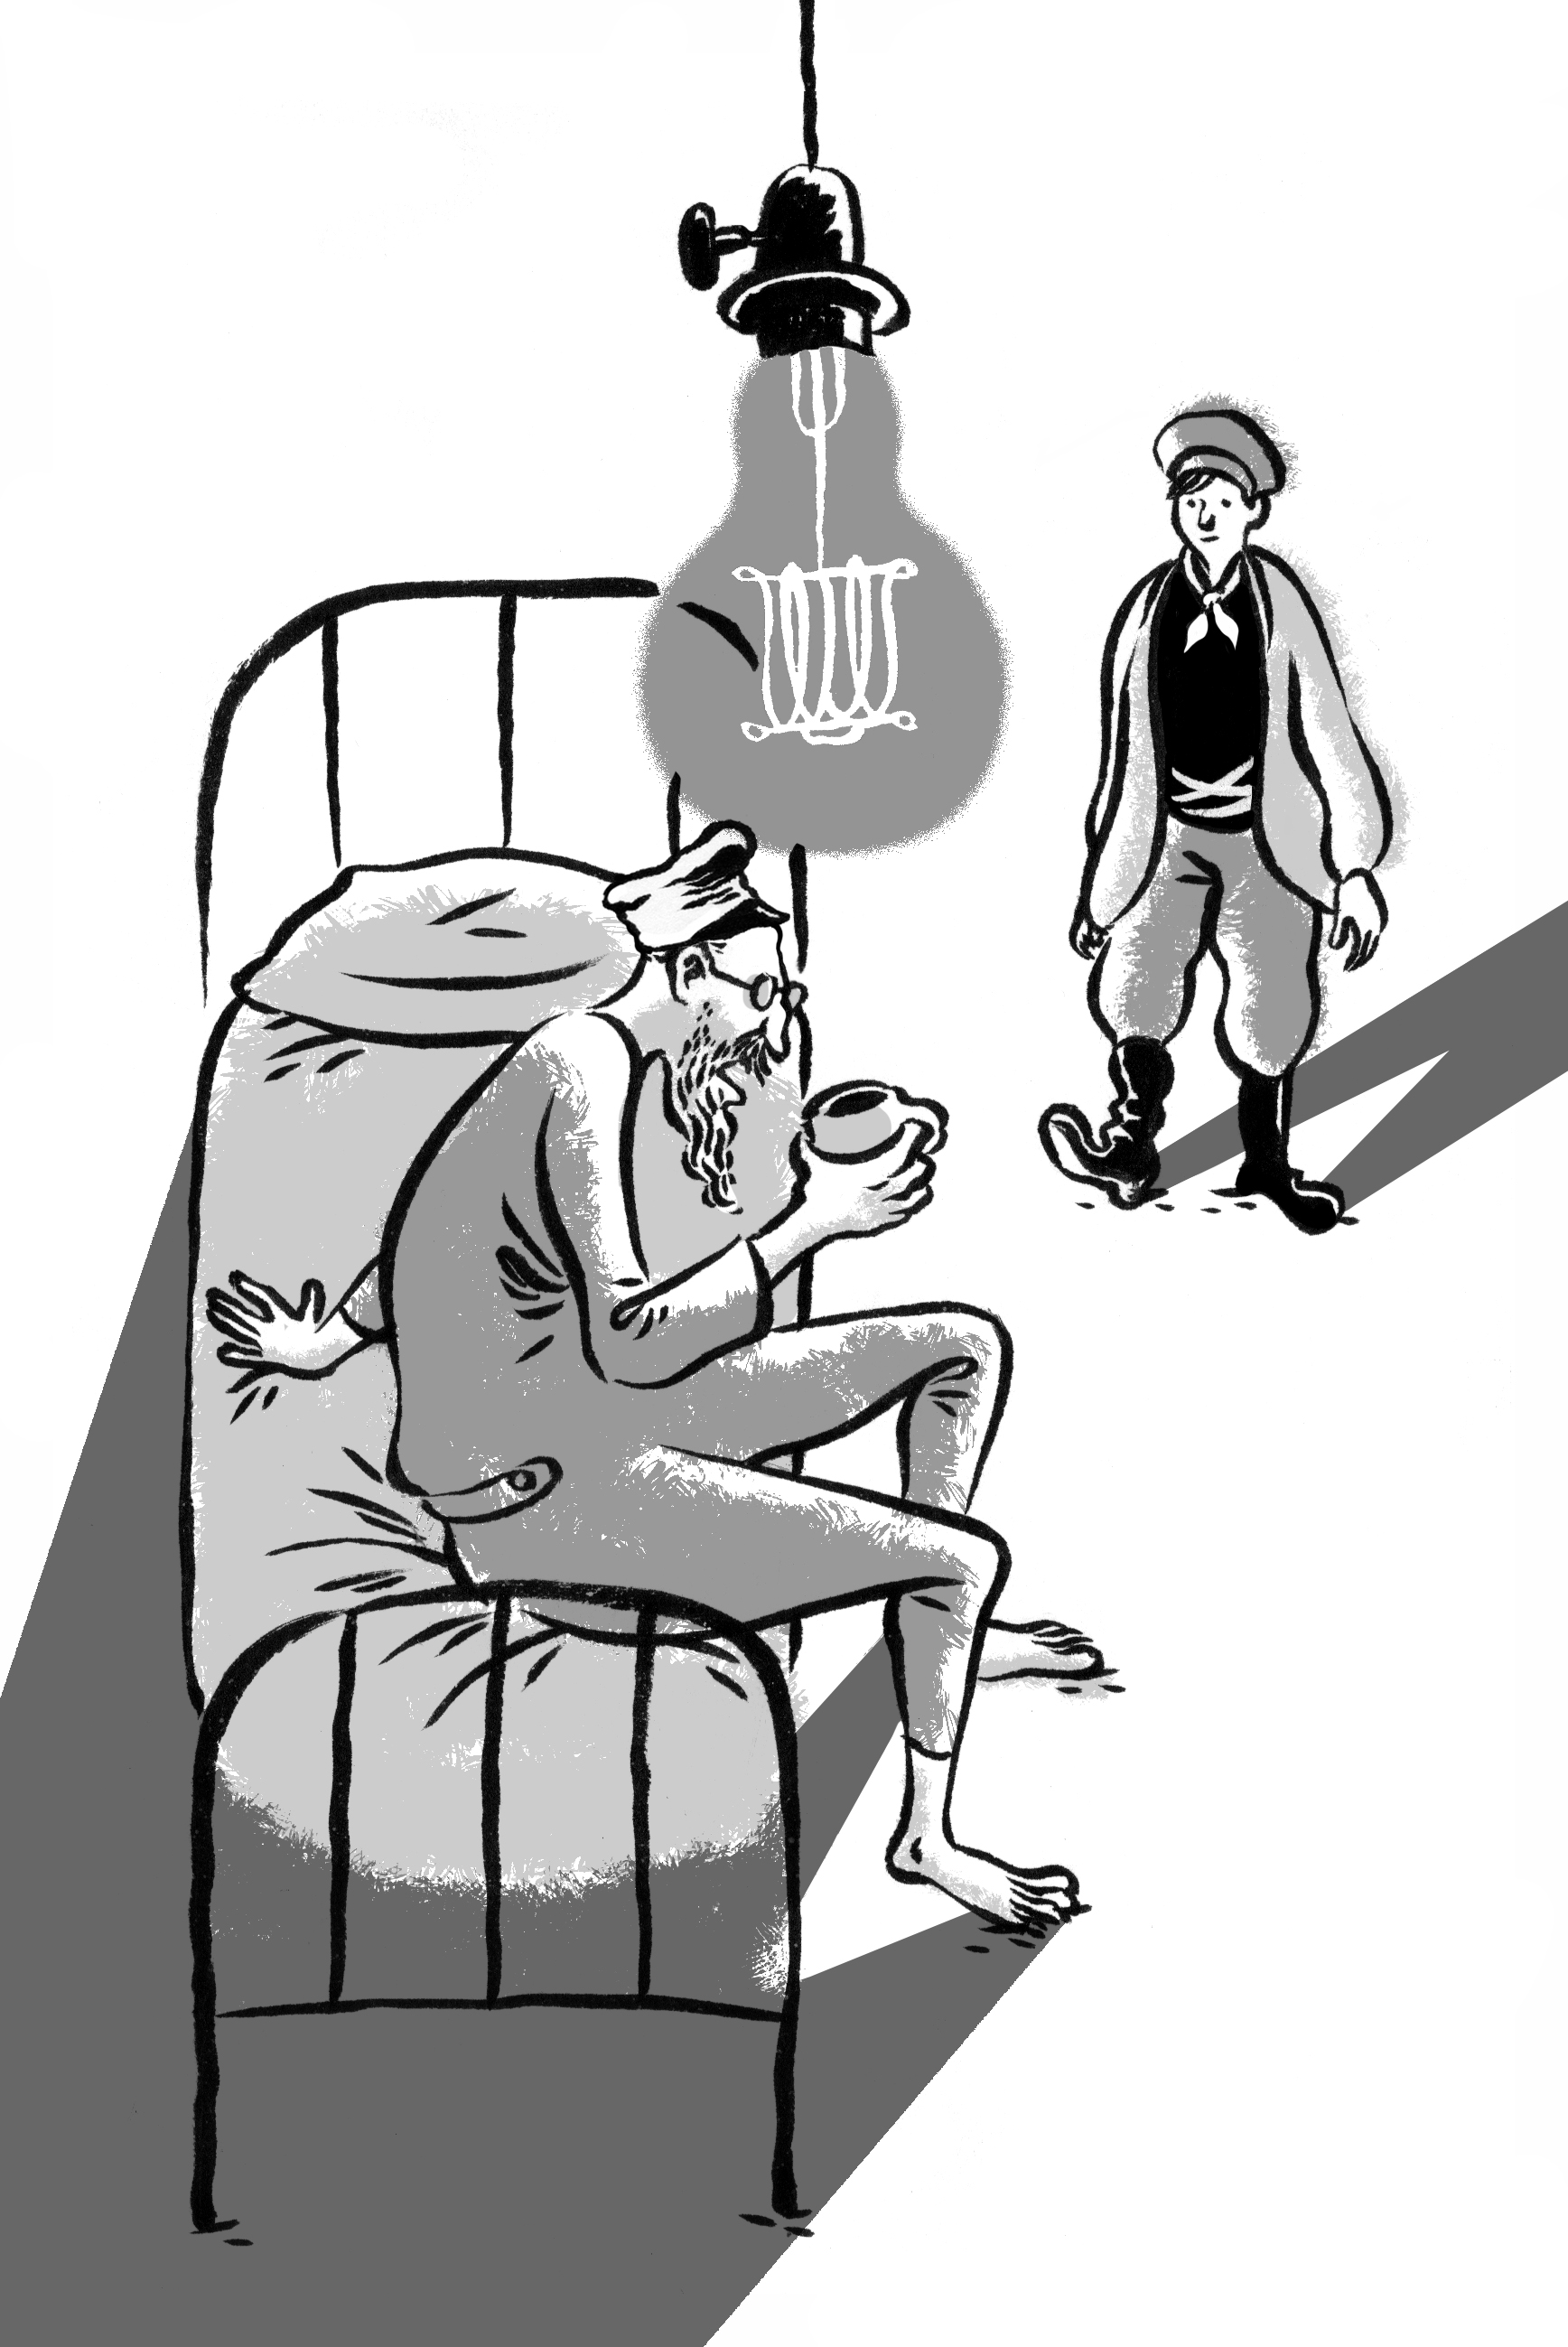
\includegraphics{./imgs/cena7.jpg}
\end{figure}

Pachka despiu"-se e não sem prazer começou a vestir o traje novo. Após
colocar camisa, calças e aventalzinho cinza, olhou para si mesmo com
satisfação, e pensou que não seria ruim passear pela aldeia nessa
indumentária. Em sua imaginação sua mãe o mandava colher folhas de
repolho para o leitão na horta perto do rio; ele caminhava enquanto
meninos e meninas o cercavam e fitavam seu avental com inveja.

Na enfermaria, entrou uma cuidadora trazendo duas tigelas de estanho,
colheres e dois pedaços de pão. Colocou uma tigela na frente do velho e
outra na frente de Pachka.

--- Coma! --- disse.

Ao olhar para tigela, o menino viu uma sopa gordurosa de repolho com um
pedaço de carne dentro, e voltou a pensar que se vivia muito bem com o
médico e que ele não era tão zangado como parecera no começo. Ficou
tomando a sopa bem devagar, lambendo a colher depois de cada trago, e,
quando na tigela não sobrou nada além da carne, olhou de esguelha para o
velho e o invejou por ainda estar sorvendo o caldo. Com um suspiro, o
menino atacou a carne, esforçando"-se para levar o maior tempo possível
para comê"-la, mas não deu em nada: logo a carne também sumiu. Restou
apenas o pedaço de pão. É insosso comer pão seco sem nada para
acompanhar, mas Pachka pensou que não havia nada a fazer e o comeu.
Nessa altura, a cuidadora entrou com tigelas novas. Dessa vez, dentro
havia carne assada com batata.

--- Mas onde está o pão? --- perguntou a cuidadora.

À guisa de resposta, Pachka encheu as bochechas e soprou o ar.

--- Ora, por que engoliu tudo? --- disse a cuidadora em tom de reproche.
--- Agora com que você vai comer o assado?

Ela saiu e trouxe outro pedaço de pão. Ele nunca na vida tinha comido
carne assada e, provando"-a, achou"-a muito saborosa. Ela desapareceu
rapidamente e do pão restou mais agora do que depois da sopa. O velho,
terminado o almoço, escondeu o pão que sobrou numa mesinha. Pachka quis
fazer o mesmo, mas mudou de ideia e comeu sua fatia.

Saciado, ele foi dar uma volta. Na enfermaria vizinha, além dos homens
que avistara pela porta, havia mais quatro. Um deles lhe chamou a
atenção. Era um mujique alto, muito emagrecido, de rosto sombrio e
peludo; estava sentado na cama e, como um pêndulo, acenava a cabeça e
agitava o braço direito sem parar. Pachka ficou muito tempo sem tirar os
olhos dele. No começo, os movimentos pendulares e ritmados do mujique
pareceram curiosos, produzidos para a diversão de todos, mas, ao olhar
para o rosto dele, sentiu"-me mal e compreendeu que aquele homem
tinha uma dor insuportável. Ao passar para a terceira enfermaria, viu
dois mujiques de rostos vermelho"-escuros, como se estivessem sujos de
barro. Sentavam inertes em suas camas e, com as fisionomias estranhas e
quase irreconhecíveis, lembravam ídolos pagãos.

--- Tia, por que eles estão assim? --- Pachka perguntou à cuidadora.

--- Rapazinho, eles têm varíola.

Ao voltar para sua enfermaria, o menino sentou"-se na cama e ficou
esperando pelo doutor, para apanharem pintassilgos ou irem juntos à
feira. Mas o médico não veio. Um enfermeiro atravessou rápido a porta da
enfermaria ao lado. Inclinou"-se sobre o paciente que tinha o saco de
gelo na cabeça e gritou:

--- Mikhailo!

Mikhailo, adormecido, não se movia. O enfermeiro abanou o braço,
desistindo, e saiu. Enquanto esperava pelo médico, Pachka começou a
examinar seu vizinho. O velho tossia e cuspia na caneca sem cessar; sua
tosse era prolongada, rangente. Pachka gostava de uma particularidade
dele: quando, ao tossir, puxava o ar, algo assobiava em seu peito e
entoava diferentes vozes.

--- Vovô, o que é isso assobiando em você? --- perguntou ele.

O velho não respondeu. O menino fez uma pausa e perguntou:

--- Vovô, cadê a raposa?

--- Que raposa?

--- A viva.

--- Mas onde estaria? Na floresta!

Passou muito tempo e mesmo assim o médico não apareceu. A cuidadora
trouxe chá e ralhou com Pachka, porque ele não tinha guardado um pouco
de pão para acompanhar; o enfermeiro tentou mais uma vez acordar
Mikhailo; do outro lado das janelas azulava, luzes se acendiam nas
enfermarias, e o médico não vinha. Já era tarde para ir à feira e para
apanhar pintassilgos; Pachka esticou"-se na cama e pôs"-se a refletir.
Recordou as balas prometidas pelo doutor, o rosto e a voz de sua mãe, a
escuridão de sua isbá, a estufa, a rabugenta avó Egórovna\ldots{} E, de
repente, ficou aborrecido e triste. Mas lembrou que sua mãe viria no dia
seguinte, sorriu e fechou os olhos.

Foi despertado por um murmúrio. Na enfermaria vizinha, alguém andava e
cochichava a meia voz. Sob a luz opaca das lâmpadas de cabeceira e das
lamparinas perto do leito de Mikhailo, três figuras se moviam.

--- Levamos com a cama ou o quê? --- perguntou uma delas.

--- É o seguinte: com a cama não passa. Arre, morreu em hora inoportuna,
que Deus o tenha!

Um pegou"-o pelos ombros, outro pelas pernas e o ergueram: os braços de
Mikhailo e as mangas de seu avental balançavam debilmente no ar. A
terceira figura --- o mujique que lembrava uma mulher --- fez o sinal da
cruz, e o trio saiu da enfermaria com um bater desordenado de pés e
pisando nas abas da roupa do morto.

O peito do velho adormecido emitia um assobio e um canto de vozes
variadas. Pachka aguçou o ouvido, olhou para as janelas escuras e saltou
da cama, apavorado.

--- Ma"-mãe! --- gemeu com voz grave.

Sem esperar por uma resposta, irrompeu na enfermaria vizinha. Lá, a
lâmpada de cabeceira e as lamparinas mal iluminavam a escuridão; os
pacientes, angustiados pela morte de Mikhailo, estavam sentados em seus
leitos, misturados às sombras e despenteados; para Pachka pareciam
maiores, mais altos e cada vez mais numerosos; na última cama, no canto,
onde era mais escuro, estava sentado o mujique agitando a cabeça e o
braço.

O menino, sem distinguir as portas, precipitou"-se para a enfermaria da
varíola, de lá para o corredor, do corredor voou para um quarto grande,
onde estavam deitados e sentados nos leitos monstros de cabelos
compridos e rostos de velhas. Ao atravessar a ala feminina, voltou a
sair para o corredor, avistou o corrimão de uma escada conhecida e
desceu em disparada. Lá, reconheceu a sala de recepção em que estivera
pela manhã e se pôs a procurar a porta de saída.

O ferrolho rangeu, veio uma lufada de ar gelado, e Pachka, aos tropeços,
saiu correndo ao pátio. Tinha só uma ideia --- fugir, fugir! Não sabia o
caminho, mas tinha certeza que, se corresse, iria sem falta parar em
casa, com a mãe. A noite estava nublada, mas a lua brilhava detrás das
nuvens. Ele saiu correndo da escadaria da entrada, contornou um galpão e
deparou"-se com arbustos desfolhados; parando um pouco para refletir,
precipitou"-se de volta ao hospital, contornou"-o e se deteve de novo,
indeciso: atrás do prédio havia cruzes brancas de túmulos.

--- Ma"-mãe! --- gritou e recuou.

Cruzando com pressa construções escuras e severas, avistou uma janela
iluminada.

A mancha vermelha e brilhante parecia assustadora na escuridão da noite,
mas Pachka, tomado de pavor, sem saber para onde correr, virou"-se na
direção dela. Ao lado da janela, havia uma escadaria coberta e a porta
da entrada principal com uma tabuleta branca; o menino subiu correndo os
degraus, olhou pela janela e foi invadido por uma alegria avassaladora.
Ali dentro avistou o médico alegre e bondoso, sentado à mesa, lendo um
livro. Rindo de felicidade, estendeu a mão ao rosto conhecido e quis
gritar, mas uma força invisível prendeu"-lhe a respiração e atingiu suas
pernas; ele cambaleou e tombou nos degraus, sem sentidos.

Quando voltou a si, já estava claro e uma voz familiar, a mesma que na
véspera lhe prometera a feira, as balas e a raposa, dizia a seu lado:

--- Mas que bobo, Pachka! Não é um bobo? Devia levar um sopapo, só não
há quem bata.

\medskip

{\footnotesize\hfill\emph{Tradução: Irineu Franco Perpetuo.}}

\chapter*{}
\label{part8}
\thispagestyle{empty}

\begin{vplace}[1.5]
{\HUGES\hfill\textbl{FIÓDOR SOLOGUB}}

{\LARGE\hfill\textlt(1863–1927)}
\end{vplace}

\pagebreak
\thispagestyle{empty}
\mbox{}
\vfill
\begin{center}
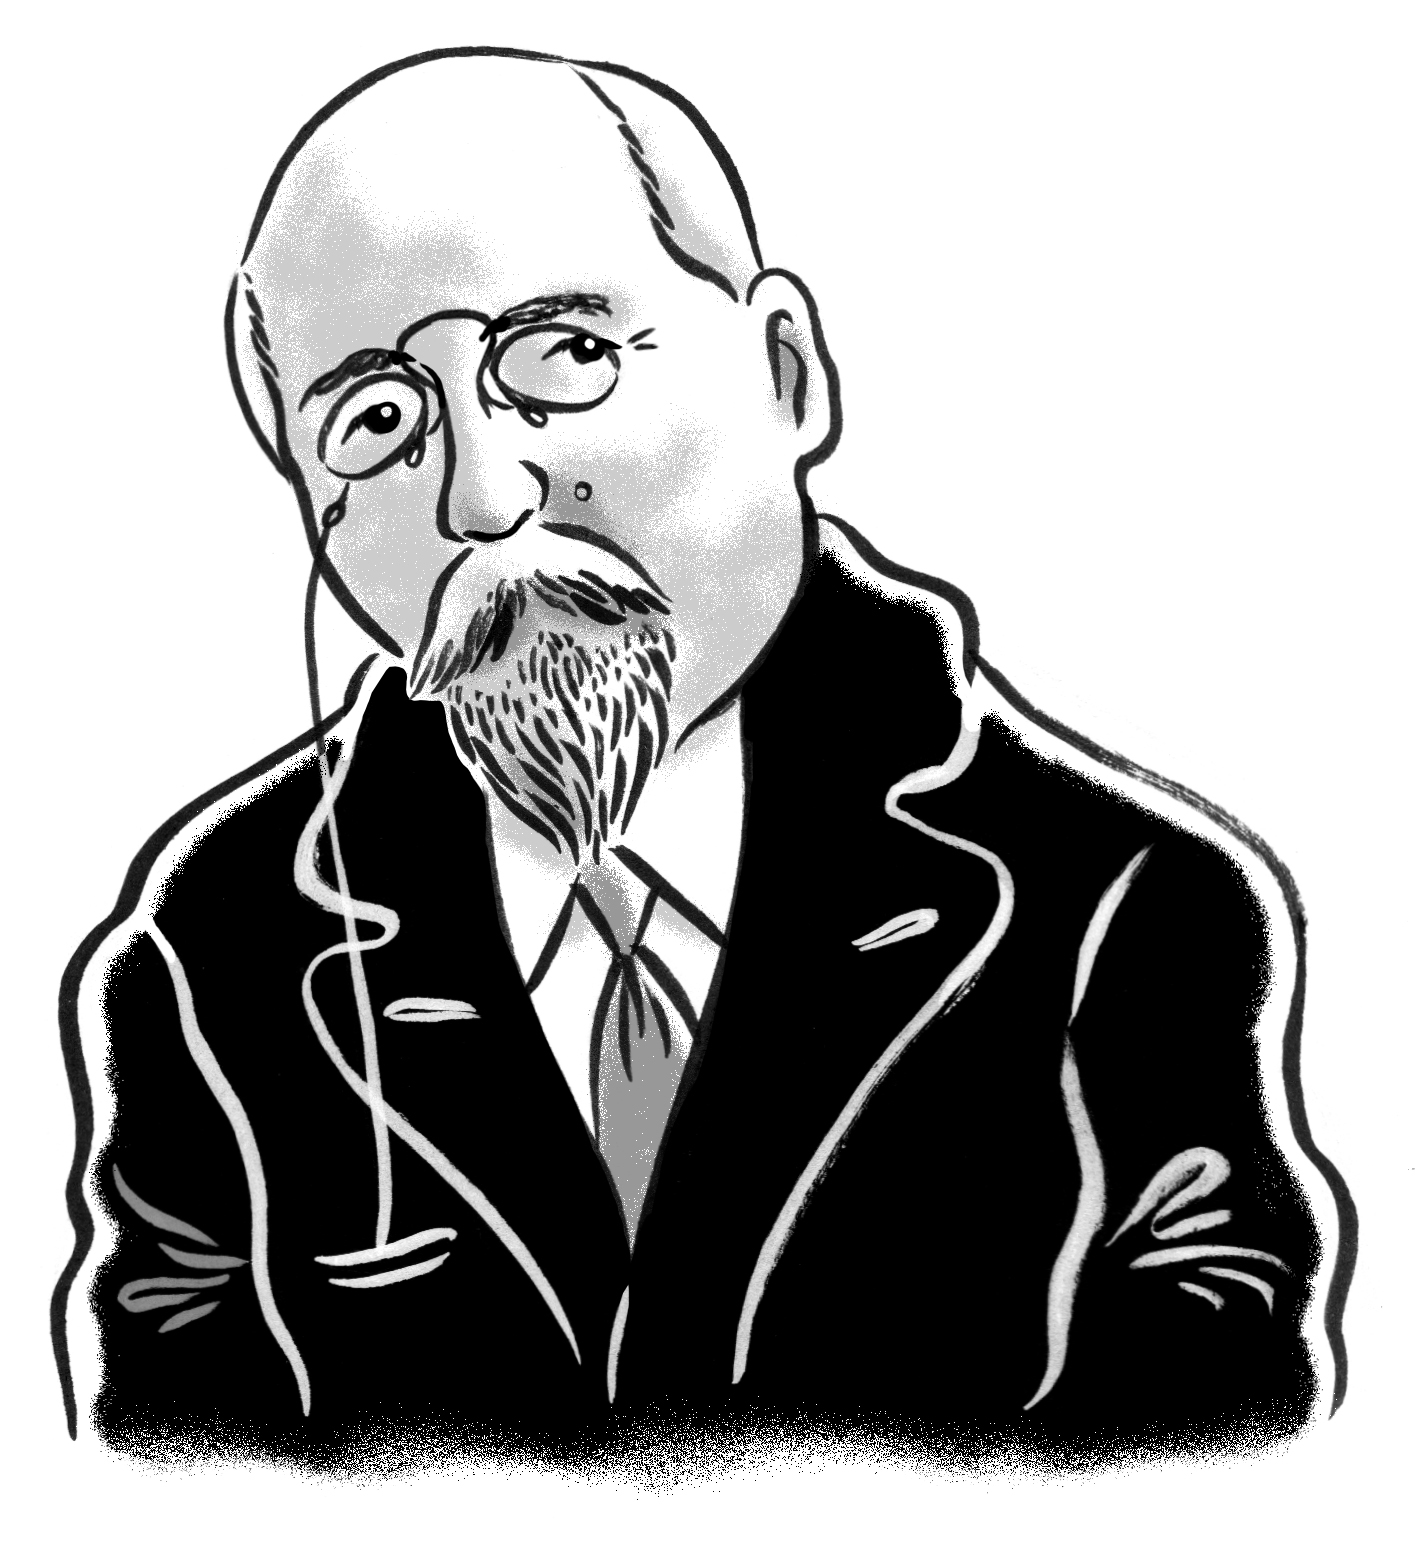
\includegraphics[width=6cm]{./imgs/autor7.jpg}
\end{center}


\chapter{Conto da filha do fabricante de caixões}

Não havia nada de estranho no fato de o jovem funcionário público Leonti
Vassílievitch Elnítski ter"-se enamorado da jovem Zoia Ilina, filha de um
comerciante local. Era uma moça instruída e de boas maneiras, havia
terminado o ginásio, sabia o inglês, costumava ler e dava aulas. E, como
se não bastasse, era encantadora. Pelo menos, para Elnítski.

Ele a visitava com prazer e logo se habituou ao que no início produziu
um efeito penoso nos seus nervos. Logo também se consolou com o
pensamento de que, apesar de tudo, Gavriil Kiríllovitch Ilin, pai de
Zoia, era o primeiro mestre da cidade no ofício.

Gavriil Kiríllovitch dizia:

--- Meu trabalho não é qualquer coisa efêmera. Para os senhores, isso
pode não ser poesia com geografia. Mas nem sequer uma pessoa passará sem
a minha mercadoria. Além do mais, meu negócio é perfeitamente limpo. O
caixão não tem cheiro, e o ar dentro de casa é forte e saudável.

Zoia amiúde ficava no depósito, o quarto onde se guardavam caixões
prontos, para qualquer eventualidade. Vestida de muitas cores e com
elegância --- sempre sobravam do serviço do pai cetim e brocado e até de
bom gosto ---, ela com frequência chamava seu amigo para ir lá.

--- Vamos ao depósito, Leonti Vassílievitch --- dizia ela ---, lá é
quente e seco, dá vontade de contar histórias. Cada tábua exala suas
fantasias.

Eles iam ao depósito. Lá Zoia narrava a Leonti Vassílievitch histórias e
contos de fada que tinha lido, mas os modificava à vontade acrescentando
suas invencionices. No início Elnítski ficava encolhido, desajeitado, e
olhava ao redor com ar sombrio, mas depois começou a expressar suas
opiniões diante de Zoia.

De vez em quando o pai da moça aparecia lá, para trabalhar ou
simplesmente para ouvir a conversa dos dois. Se ia pelo trabalho, Zoia e
Elnítski dirigiam"-se para outros quartos. Se à toa, eles continuavam a
conversar, e o pai os ouvia alisando os longos bigodes grisalhos, com os
olhos azuis brilhantes e alegres, iguais aos da filha, mas esses ainda
jovens. Se alguém observasse aqueles olhos com atenção, entenderia que
eles viram muito e habituaram"-se a observar.

Uma vez, quando os três estavam no depósito, o velho disse a Elnítski:

--- Eu vejo tudo, eu sei de tudo. Claro, como já sou muito conhecido,
não me ocupo da gente simples, porém, no que concerne aos moradores
respeitáveis da nossa cidade, eu conheço a hora e as proporções de cada
um. Tenho tudo preparado, basta o sujeito morrer. Claro, para manter as
aparências, tiro as medidas, mas vou dizer"-lhe francamente, nem
precisaria incomodar o morto. Somente fornecer o aparato conforme o
desejo dos parentes.

Leonti Vassílievitch sorria, incrédulo, e o velho prosseguia:

--- Olhe, aqui há uma pilha de caixões de vários tamanhos; cada um foi
ajustado a alguém no comprimento, na altura e em tudo. Meu olho é
certeiro e minha medição é rápida.

Zoia corou de leve e sorriu, mas Leonti Vassílievitch perguntou:

--- Que tipo de medição?

O velho explicou com prazer:

--- Levo minha Zoia à igreja, a um passeio ou ao teatro. Ela fica de pé
ao lado de quem preciso medir, e eu logo vejo as diferenças na altura e
na largura. Não erro sequer por um centímetro. Certamente, há muita
gente em nossa cidade e coincidências em medidas, e às vezes tenho
vários candidatos para um mesmo caixão. Mantenho uma lista.

Leonti Vassílievitch lembrou que, num daqueles dias, Zoia aproximara"-se
e ficara parada do lado dele, enquanto o velho fitava"-os com atenção. O
jovem sentiu um calafrio correr pela espinha. Ele olhou para Zoia com ar
de reprovação. Ela virou"-se e, com um leve movimento da mãozinha
flexível, apontou para um dos caixões.

--- Aqui está um do meu tamanho --- disse ela com indiferença.

--- E isso não a apavora? --- perguntou Elnítski.

--- Eu cresci aqui --- respondeu ela calmamente.

Nessa noite, enquanto Elnítski ia para casa, ele teve a impressão de que
nunca mais cruzaria a soleira daquele quarto. Mas no dia seguinte Zoia
levou"-o de novo para lá, e ele a seguiu, obediente. Com os olhos
tristes, observou a fileira de caixões e, esforçando"-se para falar
num tom de brincadeira, perguntou:

--- Qual deles é do meu tamanho?

Mas, com desgosto, notou como lhe tremeu a voz.

Zoia sorriu calmamente e disse:

--- Sua hora ainda demora a chegar.

Falou isso com tamanha convicção, que era como se ela soubesse. E o som
das suas palavras trouxe súbita tranquilidade à alma do jovem. Zoia
acariciou a lateral do caixão dela e disse:

--- Outra pessoa irá se deitar nele, e não eu. Quase sinto pena ---
acostumei"-me com ele, até memorizei os desenhos das tábuas.

A cada dia ficava mais claro para Elnítski que ele amava Zoia. E ele
estava certo de que ela também o amava. Seus encontros tornaram"-se mais
frequentes e alegres e suas conversas mais claras e confidentes. Às
vezes, quase sem perceber, tratavam"-se com menos formalidade. Mas ainda
não falavam do amor que sentiam. Algo impedia Elnístki. Já Zoia esperava
tranquilamente, paciente e segura de si, como se fosse de fato uma
conhecedora de todas as horas.

Uma vez Elnítski perguntou:

--- Zoia, você é sonhadora. Mas será possível sonhar com o amor neste
ambiente tão sombrio?

Zoia olhou para ele com atenção e ternura e, enquanto falava, sua voz
era doce e sonora:

--- Nos túmulos as rosas florescem e sobre seus espinhos surge o amor. A
mãe Terra transpira e nos ama igualmente quando florescemos e quando
murchamos. Ela se alegra e celebra a Deus cada vez que nasce um homem.

Numa noite de meados de dezembro, Elnítski foi à casa de Zoia. As
lâmpadas estavam acesas, fazia silêncio. Ele dirigiu"-se para o depósito.
Não viu Zoia. Passou por entre os caixões para sentar"-se perto da
lareira, aquecer"-se e esperá"-la --- na entrada tinham avisado que ela
estava em casa. Seu olhar, até então distraído, deteve"-se de repente num
caixão colocado sobre um banco: lá ele avistou Zoia, estremeceu e
paralisou.

A moça dormia diretamente sobre as tábuas do caixão --- a cabeça
repousava sobre os braços flexionados, os lábios sorriam com ternura, e
a respiração era serena e regular.

Elnítski chamou"-a baixinho:

--- Zoia.

Ela abriu os olhos.

--- Ah, é você --- respondeu ela, soerguendo"-se. --- Hoje estou muito
cansada. E, quando se está muito cansado, nada melhor do que descansar
sobre as tábuas duras.

--- Saia daí --- disse ele, sombrio.

Ele pegou"-a pelos ombros e puxou"-a para si. Ágil e com leveza, ela
saltou para o chão.

--- Por pouco não caí --- disse ela. --- Você me puxou com tanta força.
Ou será que é assim tão cruel?

--- Cruel? Por quê? --- perguntou Elnítski com a voz sufocada.

--- As pessoas são assim --- disse Zoia ---, a crueldade transparece em
tudo, de forma mais forte ou mais fraca, são apenas gradações. Uma
punhalada no seu coração ou nos seus olhos, uma mordida, um beijo ---
são diferentes elos da mesma corrente. Leu hoje sobre o que fizeram com
uma irmã de caridade?

--- O quê? Não, eu não li --- disse Elnítski.

Zoia pegou uma folha aberta do jornal \emph{O discurso}\footnote{\emph{O
  discuso} (\emph{Rietch}), jornal ligado ao Partido Constitucional
  Democrático fundado em 1906 e fechado em 1917.} e a mostrou a ele.

--- Aqui está, leia.

Ele leu e, tomado por súbita indignação, gritou:

--- Canalhas!

Zoia dizia:

\begin{figure}%[ht!]
\vspace*{-2.1cm}
\hspace*{-2.3cm}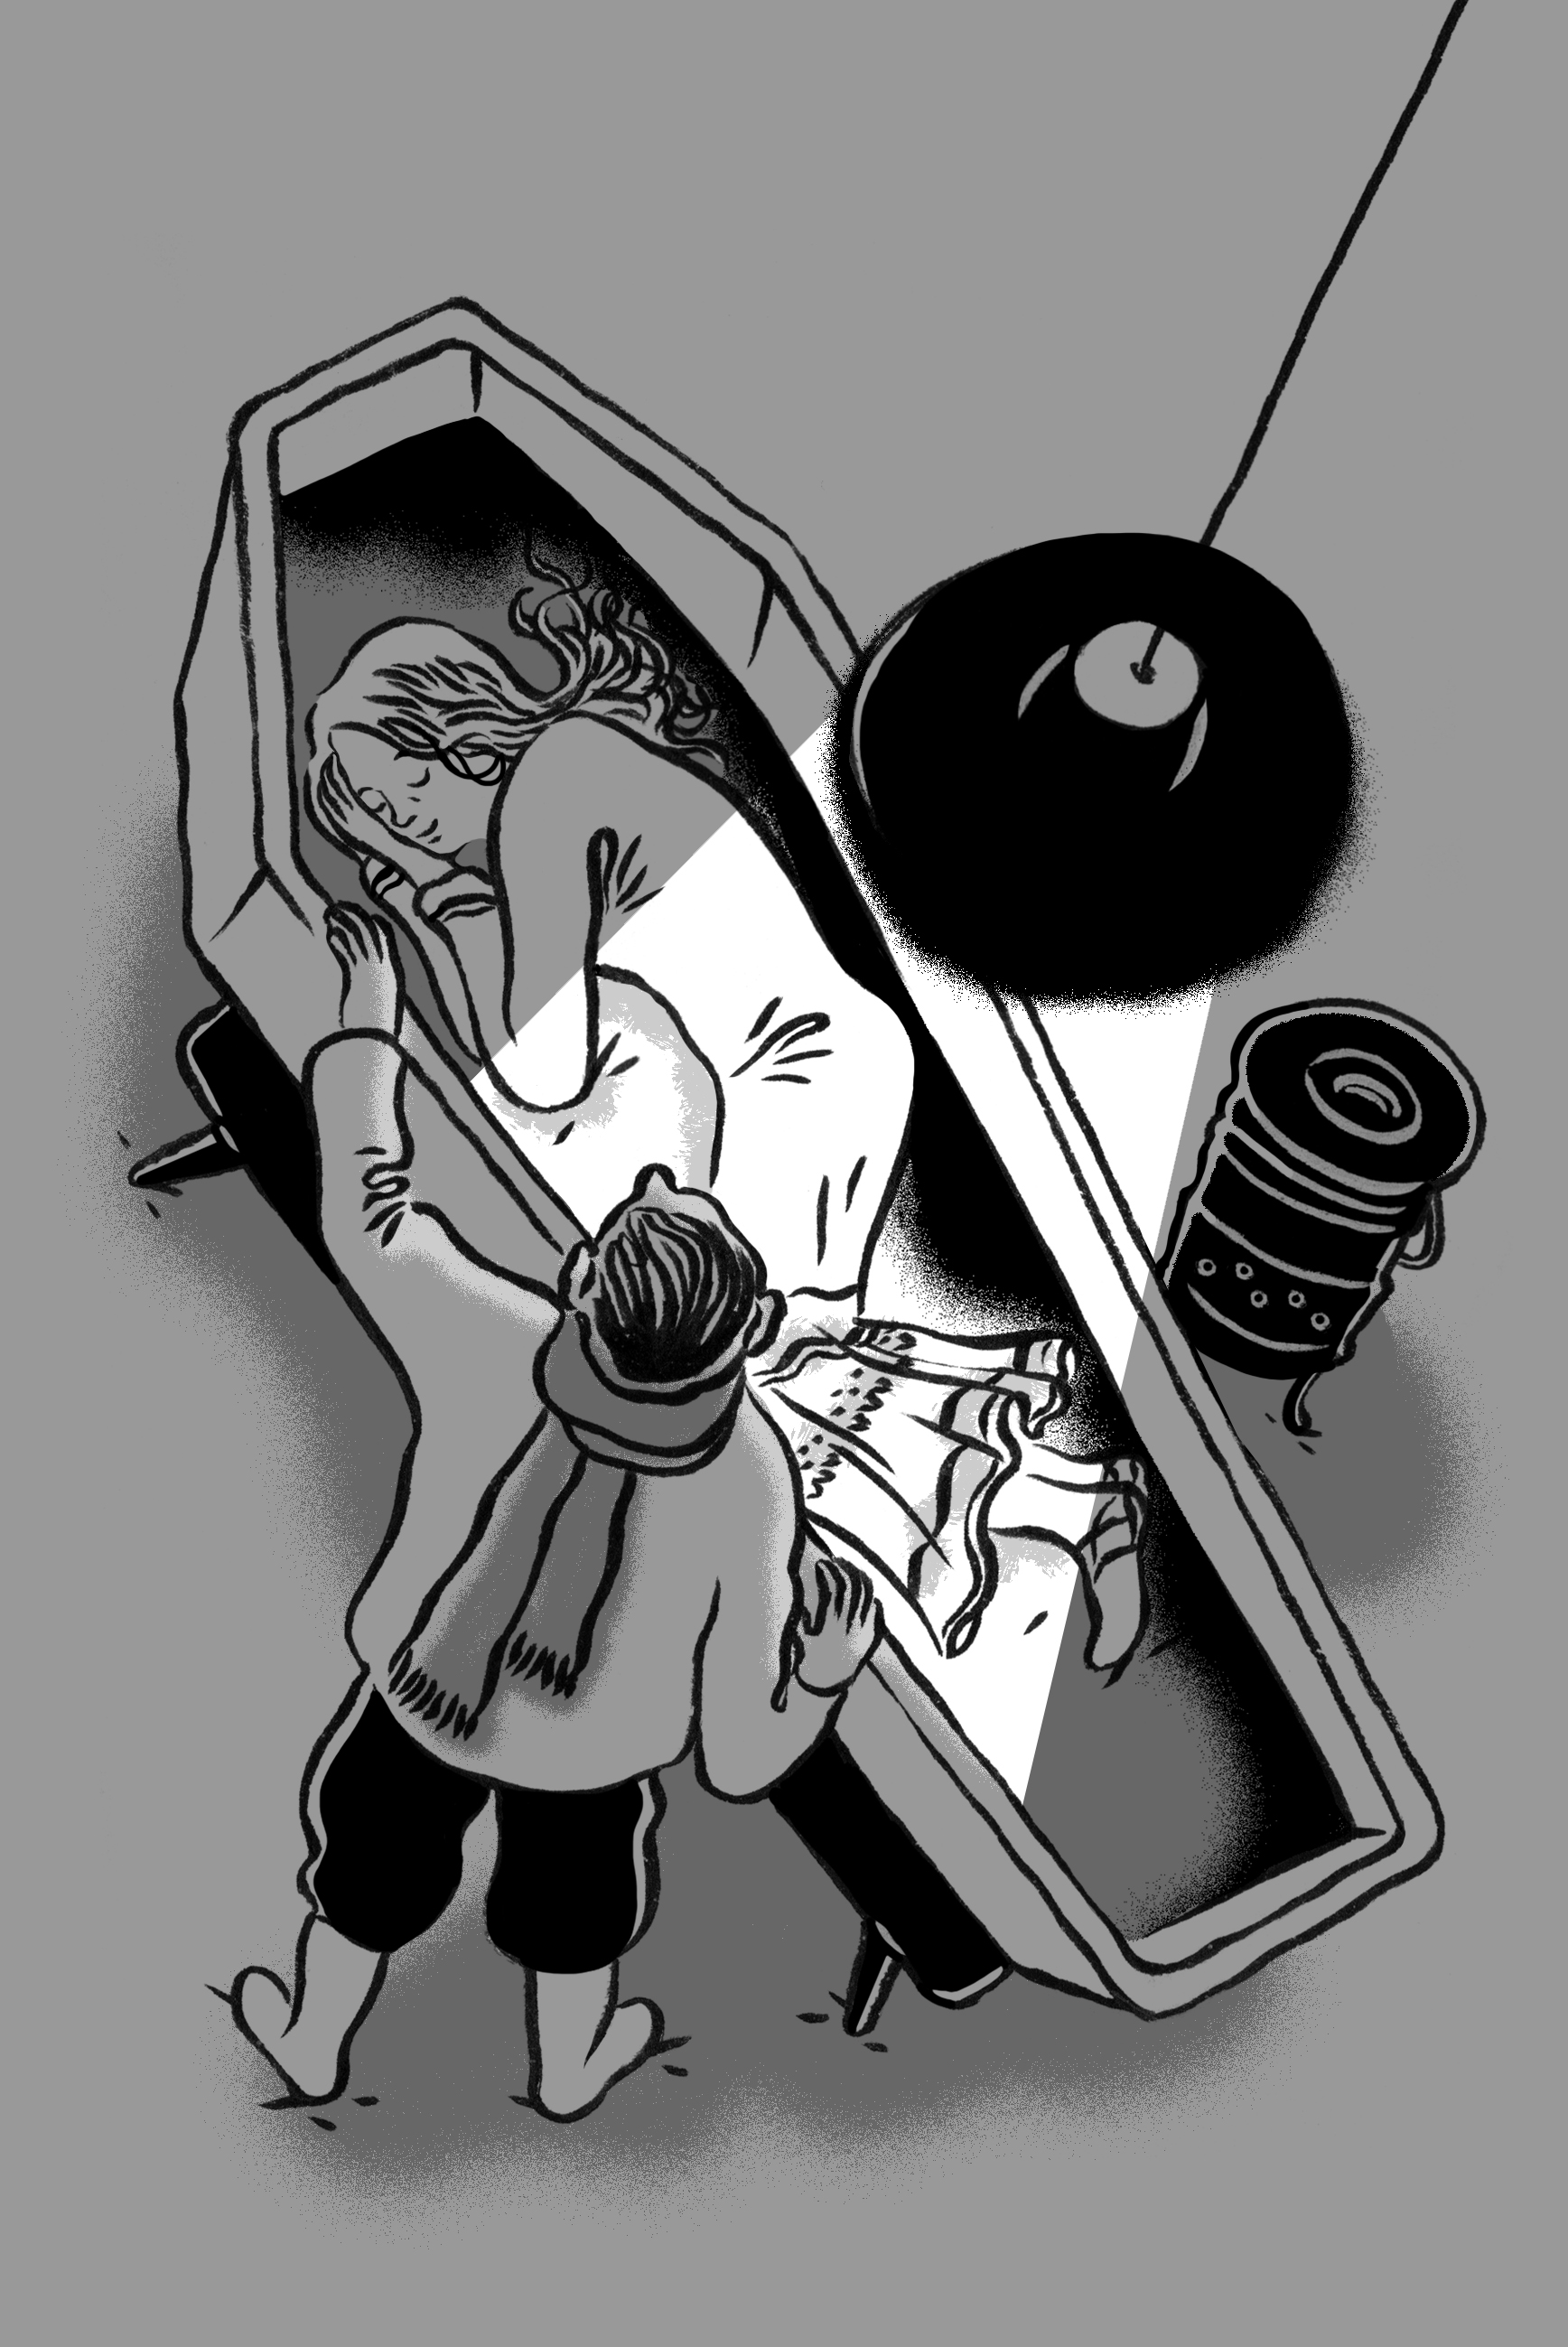
\includegraphics{./imgs/cena8.jpg}
\end{figure}

--- Apenas imagine todo o terror do sofrimento dela! Nua numa noite
gelada, amarrada a uma árvore. Lanternas apontadas para ela e dezenas de
rapazes, jovens fortes, rindo e atirando"-lhe facas. A diversão dura
muito tempo, o sangue escorre pelo seu corpo, uma faca é cravada em seu
olho --- pense, imagine! Agora, diga"-me, talvez isso tudo seja mentira,
um boato infundado, exagerado? Então como o jornal é capaz de publicar
uma coisa dessas? Ou será verdade? Então por que o mundo inteiro não
estremece, não se revolta, por que não aniquila esse grupo perverso?

--- Não é possível raciocinar dessa maneira, Zoia --- discordou
Elnítski. --- Essas pessoas perversas, criminosas, podem existir em
qualquer país.

Zoia abanou a cabeça.

--- Se isso pode acontecer em qualquer país, se uma irmã de caridade
pode ser ultrajada desse jeito por um francês ou um inglês, então isso é
o horror que pode enlouquecer um homem ou fazê"-lo amaldiçoar a
humanidade inteira. Sei que lerão isso como um crime qualquer. Alguém se
indignará um pouco, mas, para os demais, será algo indiferente. Enquanto
não mexem conosco, tudo nos é indiferente. Não passamos de animais
cruéis.

Elnítski sentiu seus pensamentos dispersarem --- decerto poderia ter
argumentado contra essas palavras absurdas e injustas, mas, sem saber
por que, não tinha vontade de falar.

Zoia olhou para ele e sorriu com tristeza.

--- Vejo que não está de acordo comigo. Escute, vou ler um conto deste
livro para você. Já o leu?

Elnítski pegou de uma mesinha de bétula que ficava perto da lareira um
livro de capa branca com desenhos verdes e dourados e leu o título:
``\emph{Tuti"-namé, contos de um papagaio.} Moscou, Editora K.F.
Nekrássov''.\footnote{\emph{Tuti"-namé, contos de um
  papagaio} (\emph{Tuti"-namé. Skázki popugaia}), adaptação, datada do
  século \textsc{xiv}, \emph{Dos setenta contos do papagaio}, escritos em sânscrito no
  século \textsc{xii}, conforme se acredita.}

--- Não, não li.

Zoia, alterando como sempre o que lia, narrava devagar e sem pausas:

--- Um rico e bondoso comerciante de Bagdá de nome Khalis havia
distribuído todas as suas posses entre dervixes pobres e órfãos. Ele não
tinha filhos, de que lhe valia o dinheiro? Mas, sabe, quando se faz
alguma coisa, é fácil deixar"-se levar pelo entusiasmo. Ele havia se
livrado de tudo, compreende, literalmente de tudo, de modo que ficou
apenas com a casa de paredes vazias, sem nada para comer nem como
comprar comida. E ele pensou: ``E daí? Vou vender a casa e doar o
dinheiro, e sobreviverei de algum jeito --- uma cabeça só não é pobre,
mas é pobre quando está só''. E logo se comprometeu com outro
comerciante: este lhe levaria o dinheiro no dia seguinte, e Khalis lhe
entregaria a casa. Aquele comerciante era avarento, percebendo que
Khalis tinha pressa em concluir o negócio, aproveitou para enriquecer de
maneira desonrosa e ofereceu muito menos do que a casa valia. Mas Khalis
não tornou a negociar. Nessa noite, ele sonhou com um homem de trajes
cintilantes. Assustou"-se muito e pensou: ``Ele veio buscar minha alma''.
Mas depois se acalmou e pensou novamente: ``E daí? Não deixarei nada
nesta terra''. Mas o homem reluzente, conhecendo os pensamentos de
Khalis, disse: ``Deus não deseja a sua morte e a sua miséria. Você
permanecerá nesta casa e terá uma esposa, e ela lhe dará filhos e
filhas. Escute, amanhã eu voltarei com a aparência de um brâmane. Você
me baterá na cabeça com um pedaço de pau, e eu me desfarei num monte de
ouro''. Assim ele disse, e Khalis guardou essas palavras na memória.
Perceba, meu querido amigo, é preciso desferir um golpe para conseguir
um tesouro. Que imagem certeira da nossa crueldade e perversidade! 

Zoia calou e então disse baixinho:

--- Acho que não vale a pena terminar a história. Você pode adivinhar
sozinho o que aconteceu. O bom foi recompensado e o avarento castigado.

Mas, entretida com o conto, ela prosseguiu:

--- Pergunte"-me: como foi castigado o avarento? Pois foi assim. De manhã
o comerciante apareceu com o dinheiro --- ele chegou cedo, para que
nenhum outro pudesse oferecer mais. Em seguida, o brâmane entrou na casa
de Khalis. Ele estava vestido com seda amarela; a face era enrugada e
amarela; o gorro de brocado de onde escapavam escassos cachos dourados
era amarelo; e as mãos eram amarelas --- era como se ele fosse todo de
ouro. E o brâmane disse: ``Khalis, mande este comerciante embora, ele
lhe oferece pouco dinheiro''. Khalis respondeu: ``Eu me comprometi com
este homem --- devo receber seu dinheiro e entregar"-lhe a casa''. Mas o
brâmane se colocou entre Khalis e o comerciante avarento, impedindo que
iniciassem o acerto. Nesse momento Khalis lembrou"-se do seu sonho, pegou
um pedaço de pau e gritou: ``Saia daqui, ou eu baterei em você''. Pois
era um homem bom, nunca levantaria a mão contra alguém sem aviso. Mas o
brâmane, insistente, não saía do lugar. Então Khalis golpeou"-o na
cabeça. O brâmane começou a brilhar e sua cabeça a tilintar, ele
encolheu"-se e, de repente, esparramou"-se numa imensa pilha de moedas de
ouro. Khalis contou noventa e nove moedas, deu"-as ao comerciante
avarento e disse: ``Você mesmo viu que eu não poderia ter agido de outra
maneira, viu como fui forçado a isso pelo ouro que veio até mim na forma
de um brâmane. Pegue este dinheiro e não conte a ninguém o que viu''. O
comerciante respondeu: ``Muito bem, desistirei do nosso negócio em troca
destas noventa e nove moedas, mas me dê este pedaço de pau''. Khalis
concordou. Ele sabia que a força não estava ali. Mas o comerciante
avarento pensou que o toco continha uma força milagrosa e que bastaria
bater com ele em um brâmane para este esparramar"-se em ouro. O
comerciante avarento foi para casa e mandou que seus empregados
convidassem todos os brâmanes que ele conhecia na cidade para um
banquete nessa mesma noite. Os brâmanes chegaram e o comerciante
deu"-lhes muito vinho. Quando ficaram bêbados, ele provocou uma briga,
pegou o toco de Khalis e começou a golpear suas cabeças. Não foi pouco o
sangue derramado, mas nenhuma moeda de ouro apareceu. Os brâmanes
levantaram uma gritaria tremenda, o povo veio correndo, o comerciante
foi pego pelos guardas e de manhã levado ao tribunal. O juiz perguntou:
``Por que você bateu nos brâmanes?''. O comerciante respondeu: ``Khalis
ensinou"-me isso''. E contou o que tinha visto na casa de Khalis. Foram
atrás de Khalis e o juiz disse: ``Escute o que este homem diz contra
você''. Depois de ouvir a história do comerciante, Khalis disse ao juiz:
``Senhor, pergunte entre meus vizinhos se alguém viu um brâmane entrando
em minha casa e pergunte aos brâmanes se um deles está desaparecido,
alguém que procuram e não encontram''. E ninguém tinha visto um brâmane
entrando na casa de Khalis, e entre os brâmanes não havia nenhum
desaparecido, ninguém que procuravam e não encontravam. O juiz ordenou
que batessem no comerciante com pedaços de pau, todo o ouro lhe foi
tomado e dividido entre os brâmanes ofendidos.

Zoia calou"-se e Elnítski disse:

--- Cada dia, Zoia, você me conta histórias. Mas sabe qual é a melhor
delas?

--- Sei --- disse Zoia ---, é a que fazemos da nossa vida.

--- Zoia --- perguntou ele ---, você me ama?

--- Não sei --- disse Zoia ---, pois você nenhuma vez me golpeou, nem na
cabeça nem no coração, para que eu me tornasse seu tesouro, o ouro de
sua vida.

Ela riu e o fitou com um olhar desafiante e insolente.

--- Como eu poderia bater em você? --- perguntou ele, desconcertado.

--- Não vai conseguir nenhum tesouro sem esforço --- respondeu Zoia.

Ela estava à frente de Elnítski, provocando"-o com aquele sorriso
insolente e com um olhar obstinado nos olhos sombrios e maldosos.

--- Como seria possível bater em você? --- perguntou Elnítski. --- Você
é mais fraca do que eu.

Ele sentiu a cabeça girar e o coração desfalecer. Foi tomado por uma
incitação maldosa. Zoia começou a rir e seu riso soava com desagradável
estridência.

--- Oh! --- exclamou ela --- não sou assim tão indefesa. Olhe, a faca
está em cima da mesa. Ela está afiada e sua ponta é fina. Se cometer um
erro, ela facilmente irá perfurar seu coração.

Ela empalideceu e, com os lábios trêmulos, começou a estender a mão na
direção da faca.

--- Bruxa malvada! --- gritou Elnítski.

Como se movido por uma força alheia, ele bateu na bochecha de Zoia. O
golpe saiu inesperadamente forte e sonoro, e Elnítski sentiu sob sua mão
o calor que exalava da face delicada da moça. Zoia agitou"-se e atirou"-se
para o lado. O jovem ficou horrorizado com o que havia acontecido.

``O que eu fiz? Eu bati na minha amada! Que desonra!'', pensou ele
rapidamente.

De repente Zoia deu um grito estridente, pegou a faca e atirou"-se contra
Elnítski. O semblante dela deformou"-se com um esgar raivoso, seus olhos
azuis pareciam presos a pequenas esferas por raios pontudos. Elnítski
olhou para ela com pavor e admiração --- Zoia nunca esteve tão bela como
nesse minuto de ira. Ele com uma mão segurou"-lhe a mão direita e desta
pegou com muito custo a faca que reluzia, virando"-a para baixo --- a
ponta já havia atingido a roupa dele e arranhado seu peito ---; a outra
mão ele lançou pesadamente contra o ombro e o pescoço dela. Furiosa, a
moça debatia"-se nas mãos dele, forçando todo o corpo contra o peito do
jovem. De repente Elnítski sentiu uma dor na perna esquerda, deu um
grito agudo e caiu arrastando Zoia consigo. Ele bateu a cabeça na
beirada do banco e, perdendo a consciência, ouviu um grito desesperado
da jovem.

Quando Elnítski voltou a si, estava deitado no sofá da sala. Zoia
ajoelhava"-se em sua frente, chorando e beijando"-lhe as mãos. O velho,
que olhava para eles com um risinho, disse:

--- Bobagem, apenas dois arranhões. Até o casamento irá sarar.

Elnítski lembrou que exatamente com essas palavras sua velha babá o
confortava na infância. Ele sorriu\ldots{}

--- Zoia --- disse ele ---, você é meu tesouro. Quando terminará de me
contar sua história?

--- Zoia é uma contadora de histórias --- respondeu o velho no seu lugar
---, contará muitas histórias aos filhos de vocês.

--- Zoia contará ao filho --- disse Elnítski baixinho --- como o pai
dele foi à guerra. Vê, Zoia, eu entendi --- pena que um pouco tarde ---
que é preciso desferir"-lhe um golpe no coração e fugir de você, fugir
para lançar golpes e triunfar.

--- Você voltará para mim --- disse Zoia com uma estranha certeza.

--- Não sei, Zoia --- respondeu ele ---, e também não faz diferença!

O velho fabricante de caixões abanava a cabeça e dizia:

--- Ainda não é hora, meus filhos, ainda chegará a hora de irem para
suas casas certinhas.

\medskip

{\footnotesize\hfill\emph{Tradução: Moissei Mountian.}}


\chapter*{}
\label{part9}
\thispagestyle{empty}

\begin{vplace}[1.5]
{\HUGES\hfill\textbl{LÍDIA AVÍLOVA}}

{\LARGE\hfill\textlt(1864–1943)}
\end{vplace}

\pagebreak
\thispagestyle{empty}
\mbox{}
\vfill
\begin{center}
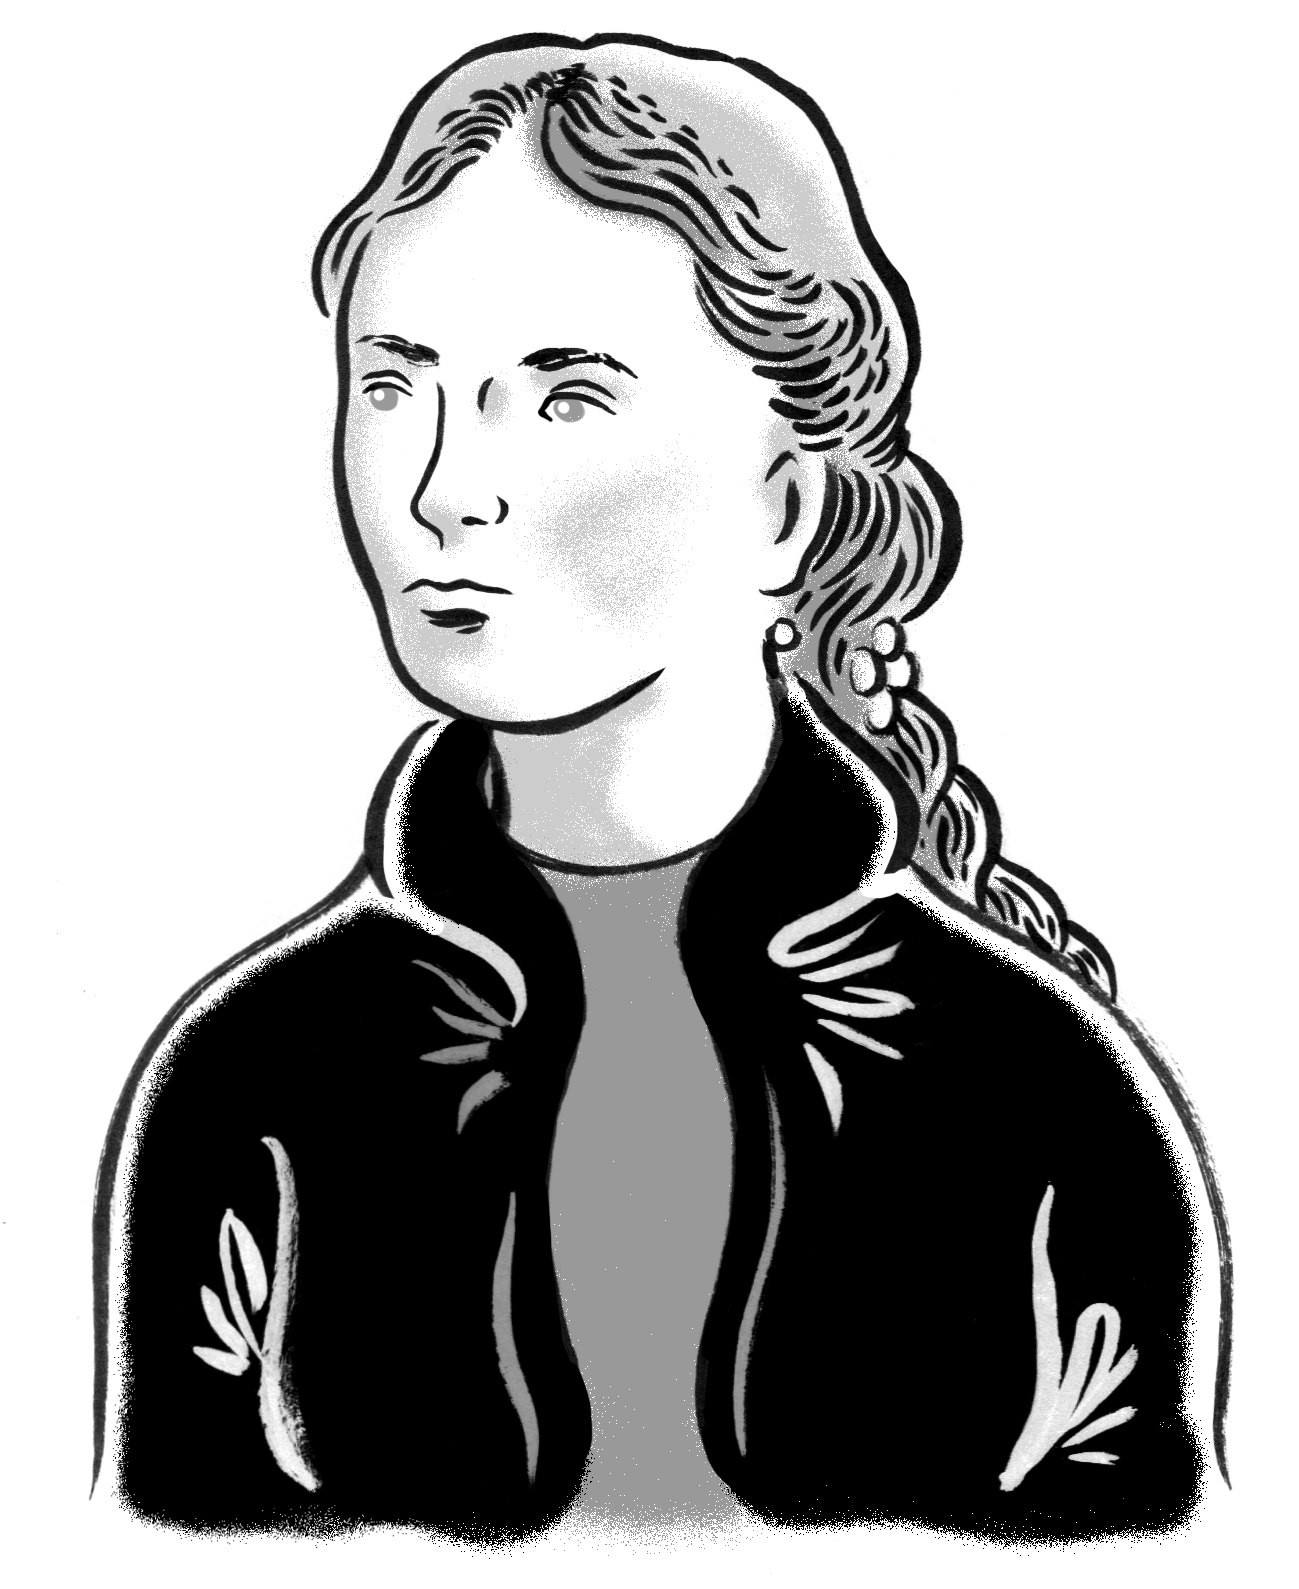
\includegraphics[width=6cm]{./imgs/autor8.jpg}
\end{center}

\chapter{Primeira mágoa}

Quando Gricha saía para o terraço, bastava entrefechar seus olhos
grandes azuis para ver, atrás dos portões abertos da estrebaria, a
traseira redonda e clara de Lóvki no estábulo, uma fileira de bridas no
tabique, e o cocheiro Ignát com um colete velho e um cachimbo
inextinguível entre os dentes. Como de costume, Gricha\footnote{Gricha, apelido de Grigóri.} não resistiu à
tentação por muito tempo: enfiou as mãos nos bolsos de suas calças
curtas, desceu pela escadinha do terraço e andou através de um grande
quintal coberto de ervas daninhas, com passos cerimoniosos de um
verdadeiro patrão.

--- E então? --- perguntou ele a Ignát, observando as coisas que lhe
eram conhecidas e queridas no galpão ---, ainda está mancando?

--- Sim, ainda está mancando! --- com total desembaraço respondeu Ignát
para manter a conversa.

--- E a coelheira, consertou?

--- Sim, agora mesmo estou consertando.

--- Olhe lá, hoje não pode dar meu Koroliók para ninguém!

--- Mas será que isso depende da minha vontade? Dirão: ``É preciso ir
até a estação ou até a vila, atrele já Koroliók'', e eu terei que
atrelá"-lo.

--- Não é justo! Sempre o meu cavalo, sempre o meu\ldots{} --- resmungando,
notou o menino. --- Colocou a aveia para ele?

--- Como é que eu pegaria a aveia sem ordem? --- respondeu Ignát, e seu
rosto barbudo, geralmente fechado, assumiu uma expressão maliciosa. ---
O patrãozinho não mandou.

--- Está sem aveia! --- gritou Gricha em desespero, e de raiva lágrimas
lhe surgiram nos olhos.

Ignát ria alegre e carinhosamente:

--- Veja que cabeça quente! Realmente um cabeça quente --- dizia ele
para tranquilizá"-lo. --- Fique calmo: não vou magoar seu Koroliók.
Tomarei de outro, mas Koroliók será plenamente satisfeito. Não se
preocupe, meu amigo.

Ele espiou com ternura os olhos do menino e lhe acariciou a cabeça com a
mão áspera e grossa. Gricha se tranquilizou e iniciou sua ronda
habitual. Sentou em todas as carruagens, uma por uma: subia nas boleias
e de passagem fazia observações.

--- Que telega excelente! --- disse ele em tom de entendedor.

--- Não posso me queixar dela! --- respondeu Ignát, dando aprovação.

--- Esta carroça de carga\ldots{} deve ser resistente, não é?

--- Vai se sujar de breu, traquinas! --- preveniu o cocheiro. --- A babá
vai ralhar com você.

--- Está bem. Não vou me sujar --- respondeu Gricha calmamente.

Ignát trabalhava na propriedade fazia menos de um ano, mas muito
rapidamente se aproximou de seu pequeno senhor, e entre eles se
estabeleceu uma estranha e sincera amizade.

--- Agora eu vou lhe contar como era a vida na casa dos senhores
Lukhkovski --- começou Ignát. --- Eles tinham um cavalo\ldots{}

--- Você morava com eles antes de nós?

--- Não. Antes eu morava aqui com um comerciante\ldots{} Certamente, por
necessidade\ldots{} Se não fosse a necessidade, eu não moraria com ele nem um
único dia. E fui levado para o tribunal! E a troco de que fui a
julgamento? Será que peguei o que não era meu?

--- Será que o comerciante queria que fosse julgado?

--- Como não?! Ele mesmo fez a queixa. Como se eu tivesse tomado dele um
cavalo e uma telega. Não me pagava o ordenado fazia um ano e também não
me deixava partir. ``More aqui!'' Eu e minha mulher pensamos assim ou
assado. Seria melhor aproveitar, já que não tínhamos
passaporte.\footnote{Na Rússia, o passaporte é o documento de
  identidade, contendo sexo, estado civil, registro de moradia, etc.} O que podia fazer? De noite, eu e Matriona atrelamos o
cavalo à telega e\ldots{} partimos para casa. Será que deveríamos percorrer a
pé, com uma criança pequena, os sessenta quilômetros? Quando o
comerciante se deu conta, tínhamos desaparecido, sem deixar vestígios. O
cavalo eu devolveria, não ficaria com ele. Mas o comerciante, veja só,
ficou furioso por ter perdido o trabalhador gratuito e foi ao tribunal
apresentar uma queixa; e, assim, diz que roubamos.

--- E você foi julgado?

--- Dizem que julgaram.

--- Mas como assim?

--- Assim mesmo! --- respondeu Ignát vagamente; suas sobrancelhas densas
franziram"-se, preocupadas, e seu rosto por muito tempo adotou uma
expressão carrancuda, quase sofredora.

--- Mas poderia ter dito que não teve culpa --- aconselhava Gricha com
ar sério.

--- Será que me perguntaram? E onde está ela, meu amigo, a verdade?
Julgaram, julgaram e fizeram de mim um ladrão. É assim!

--- Como fizeram? --- avidamente indagou o menino.

--- Fizeram e pronto! --- respondeu Ignát, com o cenho franzido e um
sorriso amargo.

E a conversa, como às vezes acontecia, tomou outro rumo.

--- Será que a Matriona é sua esposa? --- perguntou Gricha.

--- De quem mais seria? --- respondeu Ignát, em tom bondoso.

--- Por que, em vez de ficar com você, ela está sempre na casinha da
adega assando os pães?

Ignát sorria.

\begin{figure}%[ht!]
\vspace*{-1.6cm}
\hspace*{-2.3cm}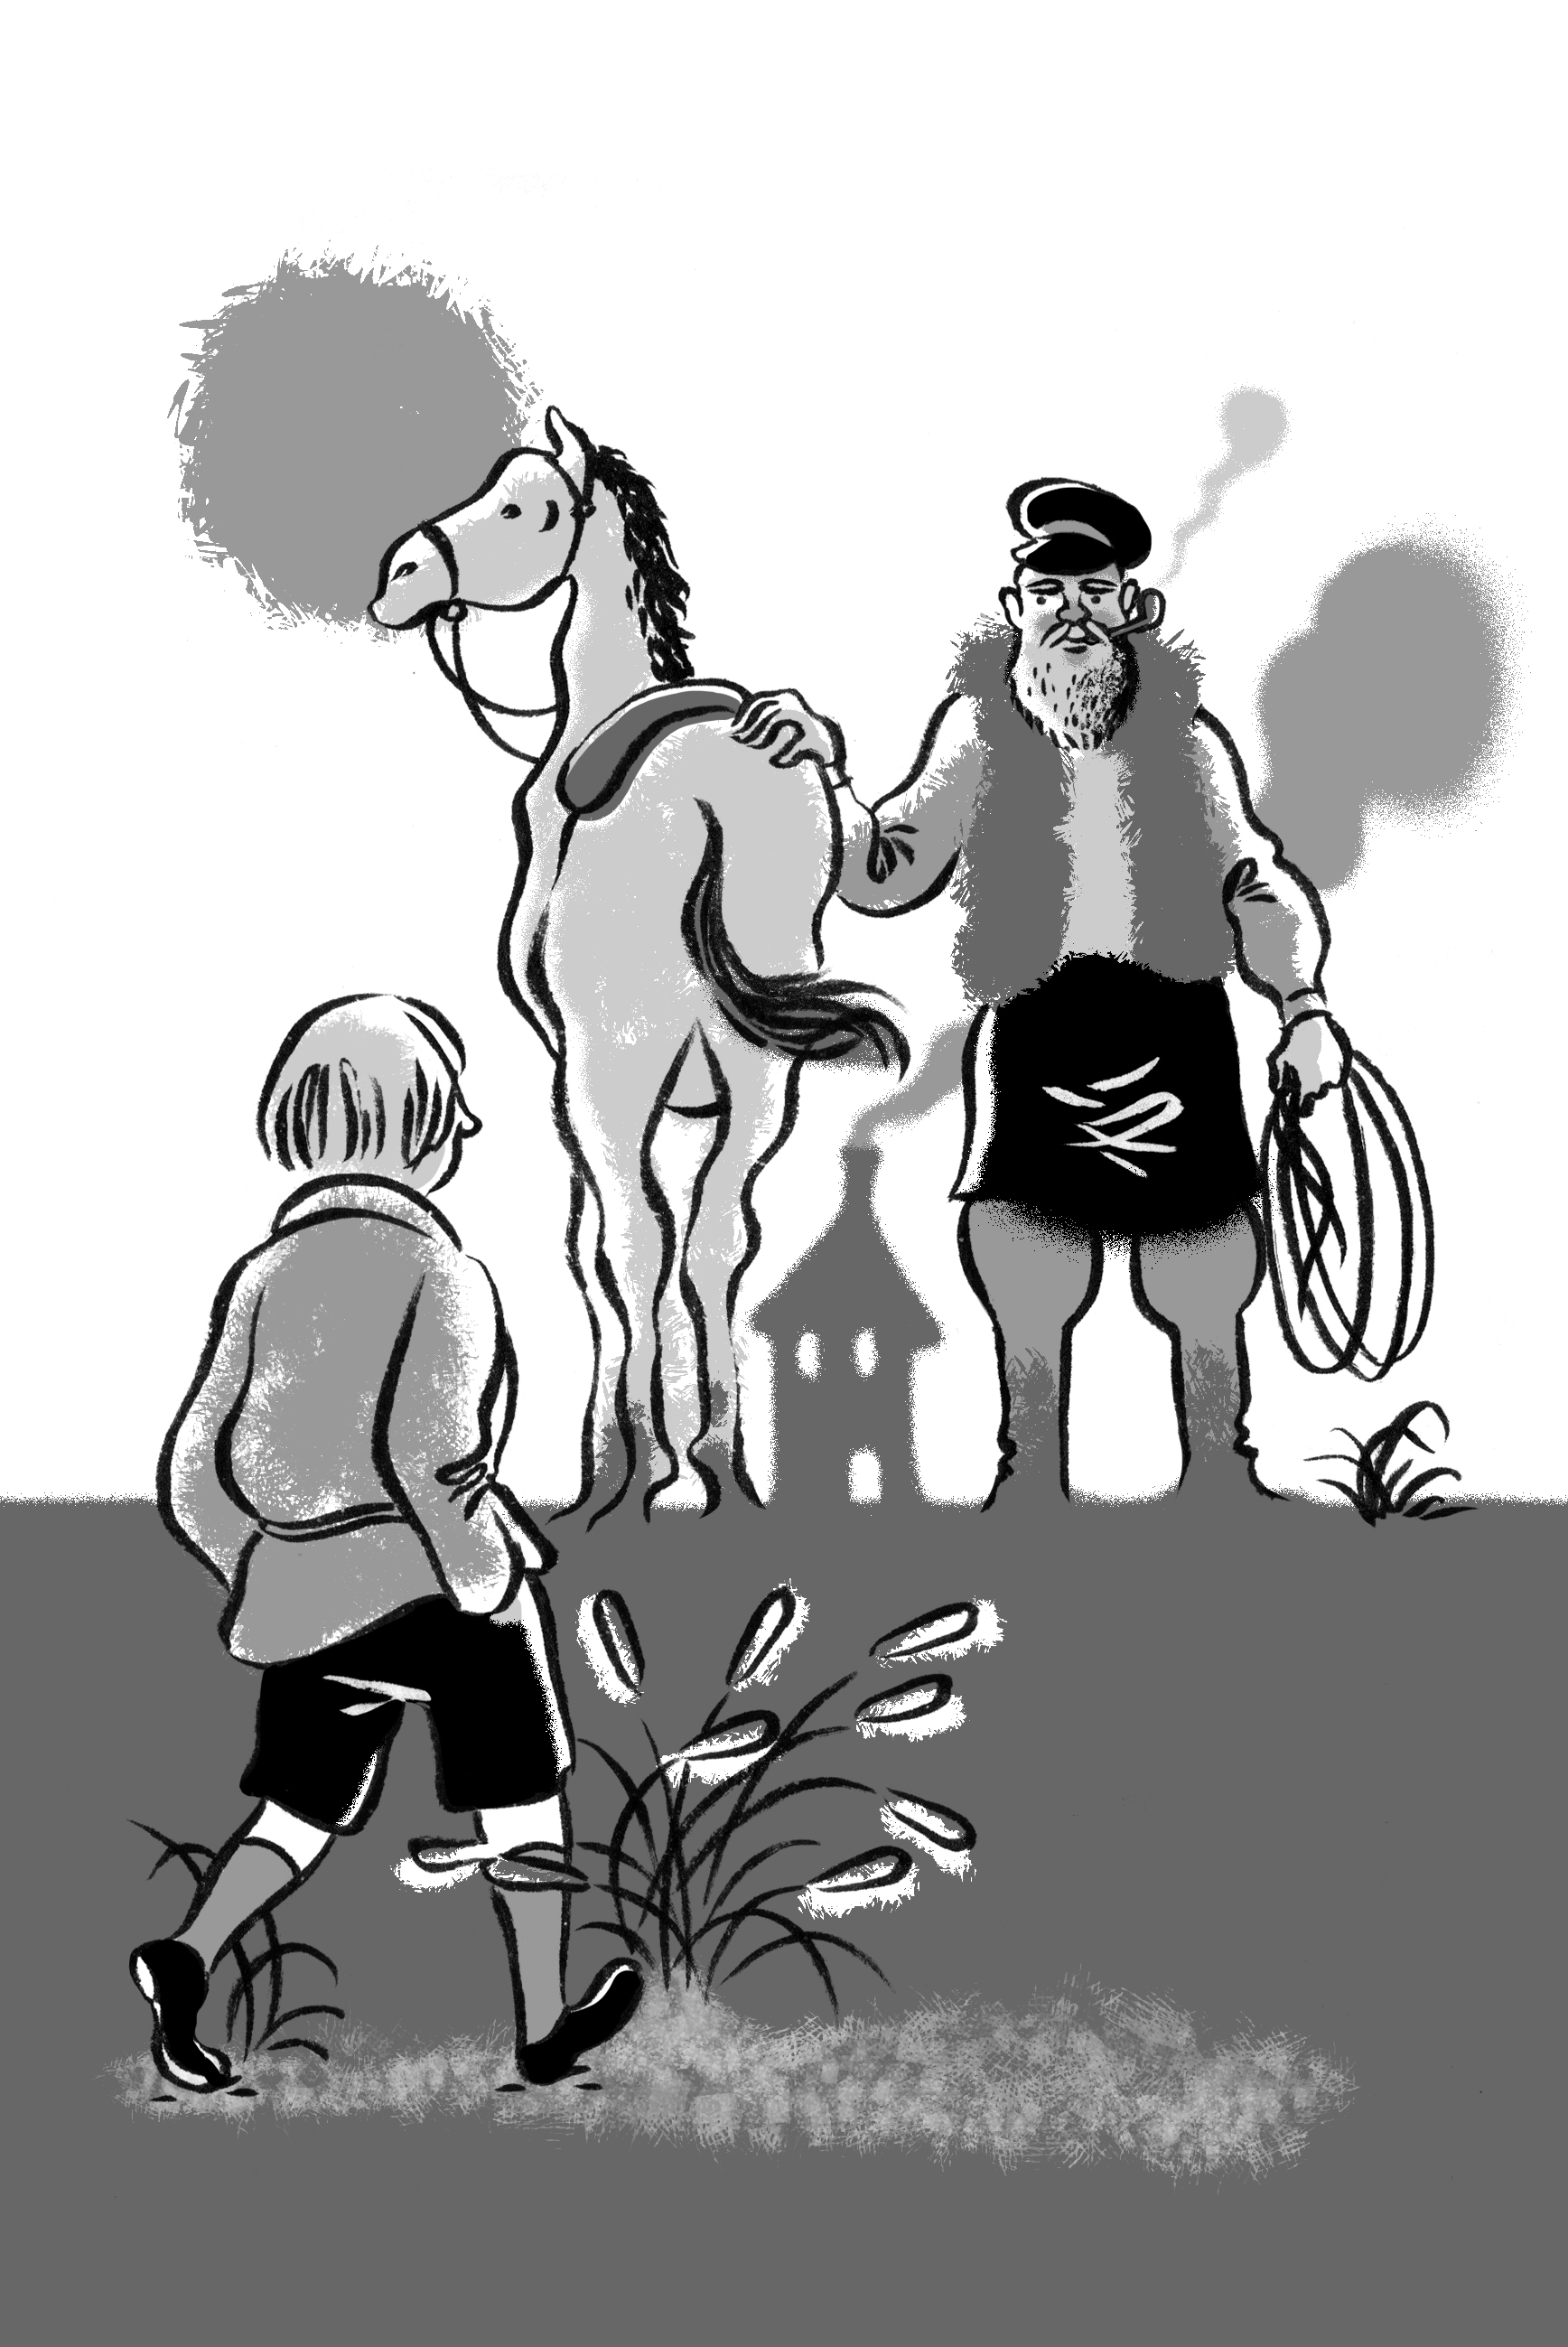
\includegraphics{./imgs/cena9.jpg}
\end{figure}

--- E o que ela faria aqui comigo? Será que contaria contos de fadas
para mim?

--- E o que os contos de fadas vieram fazer aqui? --- retrucava o menino
ardentemente. --- Minha mãe não conta os contos de fadas para meu pai e
vive assim\ldots{} E a Polka, quer dizer que é sua filha?

--- Quer dizer que é minha filha.

--- Mais crianças vocês não tiveram?

--- Não, nenhuma mais.

--- Por que não tiveram mais?

Ignát ria e balançava a cabeça.

--- Só me faltava mais uma criança! --- dizia ele.

--- Por que está rindo? --- continuava Gricha, um pouco ofendido,
explicando o seu raciocínio. --- Meu pai e minha mãe têm três
crianças\ldots{} Ignát! --- ele repentinamente perguntou ao seu amigo em tom
afável, fitando"-o nos olhos ---, quando partirmos para a cidade, você
cuidará do meu Koroliók?

--- Cuidarei, cuidarei! --- prometeu Ignát. --- Apenas, meu amigo,
talvez eu mesmo vá embora antes.

--- Para onde? --- o menino perguntou, surpreso.

--- Mas\ldots{} para aquele lugar! --- respondeu Ignát com seu modo
misterioso de sempre.

A conversa afetuosa entre os dois amigos foi interrompida, como não raro
ocorria, pela velha babá.

--- Será que o menino Gricha está aqui? --- perguntava ela, espiando o
galpão. --- Francamente --- continuava ela, mal"-humorada ---, é filho de
patrões e não sai da estrebaria. Vou me queixar a sua mãe! Veja só:
achou alguém para ser seu amigo. Vá imediatamente daqui, vá. E você,
inútil --- dirigiu"-se a Ignát ---, em vez de criar juízo na criança,
fica atraindo"-o para cá.

--- Qual é o problema, Anna Guerássimovna, eu não faço nada de errado
--- Ignát se isentava confusamente. --- Se eu ensinasse coisas ruins
para ele\ldots{}

--- Só nos faltava ter você como professor --- notava a babá com desdém.
--- Vá, traquinas, vá!

Gricha obedeceu, mas, para mostrar seu descontentamento, andava não ao
lado da babá, mas atrás dela, e enchia as bochechas de ar
exageradamente\ldots{}

--- Por que está ofendendo Ignát? --- finalmente ele perguntou,
lacônico. --- Que mal ele lhe fez?

--- Mas será que ele é companhia para você? --- a babá retrucava
ardentemente. --- Ainda se diz cocheiro. Só se for na palavra. Será que
antigamente os cocheiros eram assim? Não passa de um mujique
desajeitado. Anda de cabeça baixa, a cara cheia de cabelos, mal se pode
ver os olhos.

--- Está mentindo! Dá para ver! --- gritava bravamente o menino.

--- Obrigada, meu bem, muito obrigada, senhorzinho, por ter trocado sua
velha babá por um mujique! Um mujique desajeitado se tornou mais querido
do que sua babá! --- dizia ela com um tom de ofensa. --- Obrigada, muito
obrigada, meu caro!

--- Mas será que eu disse isso? Ora essa! --- Gricha se defendia com
lágrimas na voz.

Essas briguinhas recorrentes terminavam sem tardar em plena
reconciliação, mas não sem deixar vestígios: a afeição proibida começou
a adquirir o valor e a força de tudo o que é proibido. Mais do que
nunca, Gricha era atraído para a companhia de Ignát, mas, temendo magoar
a babá e provocar seu ciúme legítimo, o menino usava da astúcia e
comprava a velha com carinhos. Ficava nervoso, ardendo de alegria e
emoção, quando conseguia enganar a vigilância da babá e ia se esconder
na escuridão salvadora do galpão de carruagens. Nesses momentos, ele de
novo conversava, fazia perguntas, enfiava"-se em todos os lugares,
seguido por Ignát, cujos olhos sombrios e tristes, sob sobrancelhas que
caíam desordenadamente, refletiam uma estranha ternura.

--- Está vindo, Anna Guerássimovna está vindo! --- ele sussurrava às
vezes, sorrindo maliciosamente. Gricha se assustava e depois ambos riam.

\asterisc

Gricha praticamente via o pai e a mãe somente à mesa de jantar. O pai
estava sempre ocupado, e a mãe ficava dias inteiros em seu dormitório
por considerar"-se fraca de saúde. Quando não lhe doía a cabeça, doía
outra parte do corpo, o que a fazia não suportar a companhia ruidosa de
crianças e mesmo a claridade da luz do dia. Quando Gricha tinha a ideia
de visitá"-la, ela o acariciava, beijava"-o impetuosamente, repetidas
vezes, e, em seguida, pedia que ele se retirasse e não a incomodasse.

Às vezes, como dessa vez, Gricha resistia.

--- Mamãe --- dizia ele ---, vou ficar sentado quietinho, bem quietinho.

Ele se sentou na poltrona e apoiou as mãos nos joelhos.

--- Você está se sentindo bem? --- a mãe perguntou com preocupação.

--- Sim --- dizia ele distraidamente, ocupado com alguma ideia intrusa
que logo seria substituída por uma que o interessava; o menino falava
aos sussurros, para não perturbar a disposição geral de silêncio e
tranquilidade.

--- Mamãe --- sussurrava ele ---, por que, quando faz calor, a pessoa
fica sempre suada?

--- Você está com calor? --- perguntou a mãe.

--- Estou com calor\ldots{} Acha que por estar usando duas camisas?

--- Será que está usando apenas uma?

--- Sim, apenas uma! Veja! --- Gricha dava gritinhos sonoros e,
desabotoando a gola de sua \emph{kossovorotka}\footnote{\emph{Kossovorotka,}
  camisa típica russa com gola que se abotoa de lado.} de chita,
mostrava o peito nu.

A mãe franziu o rosto de maneira doentia.

--- Por que você está gritando? --- ela o recriminou.

--- Ah, eu esqueci! --- o menino falou culpadamente e se calou. ---
Mamãe --- sussurrou de novo no minuto seguinte ---, diga, para que serve
o rabo?

--- Que rabo?

--- O dos cavalos, dos cachorros?

--- Como para quê? É um simples rabo. Assim foi concebido.

--- Acontece que não é tão simples! E afugentar as moscas? Com que
afugentariam as moscas?

A tagarelice do menino começou a irritar a mulher nervosa, mas ela
suportou em silêncio, certa de que ele mesmo ficaria entediado na
penumbra e iria embora. Mas Gricha deslizou pelo respaldar da poltrona,
deitou"-se de costas no assento e levantou as pernas, cruzando uma sobre
a outra.

--- Mamãe --- começou ele de novo ---, e você sabe de onde vêm as
pulgas?

A mãe franziu o rosto, enojada, e fechou os olhos.

--- Ora, Gricha! Que conversa é essa?!

--- Das coelheiras dos cavalos. Se pulgas aparecerem, é preciso jogar as
velhas coelheiras fora e as novas\ldots{}

--- É isso que dá passar o tempo todo nos estábulos! No outono
contratarei uma governanta. Tenho vergonha de você!

--- Por que tem vergonha de mim? --- perguntou o menino, surpreso.

--- Está bem, vá embora. Vá ver a babá e suas irmãs. Você está sempre ou
sozinho, ou com mujiques.

Gricha suspirou profundamente, levantou"-se da poltrona sem vontade e
suspirou de novo: ele ainda não estava pronto para deixar o quarto
fresco e a mãe, a quem amava ternamente, mesmo que ela fosse assim tão
triste e doente.

--- Beije"-me! --- a mãe disse baixinho.

O menino começou a beijá"-la, cheio de ternurinhas, esfregando seu rosto
no dela, enquanto ela apalpava sob a camisa os ombros pontiagudos do
filho e adotava um tom queixoso.

--- Meu filho, você é tão magrinho, tão pálido! Gricha, por que você é
assim?

--- São as travessuras! --- o menino respondeu por hábito, mas a ternura
compassiva da mãe atuava sobre seus nervos e o tornava mais indulgente.

--- Meu filho, você é tão pobrezinho! Para você, a vida não é fácil! Meu
menino, você tem sempre uma tristeza na alma!

Eis que, tocado pela piedade dela e por palavras que ainda não lhe eram
conhecidas, Gricha de repente pôs"-se a soluçar no ombro da mãe.

--- O que você tem? --- indagou ela, assustada, tocando na cabeça do
filho para saber se estava febril.

Mas Gricha subitamente se acalmou e retirou"-se. Mal deu tempo de chegar
até a porta, já tinha se esquecido das lágrimas vindas sem motivo,
entretendo"-se com um pensamento novo e interessante. Em seu peito algo
ainda estremecia e soluçava, mas ele já apalpava alegremente um pedaço
de barbante esquecido no bolso, imaginando como faria melhor proveito
dele.

\asterisc

Enquanto isso, a primeira mágoa séria da vida do menino estava prestes a
cair sobre sua cabeça.

Em uma manhã, o pai, sem tirar os olhos do jornal, disse à mãe através
da mesa:

--- Sim\ldots{} está sabendo? Vieram buscar o Ignát!

--- Já vieram? --- a mãe perguntou, assustada, e, como que avaliando
algo, baixou na mesa a xícara de chá não bebida até o fim.

--- Será que nada pode ser feito? Eles têm filhos --- disse ela,
baixinho.

--- O que você sugere? --- o pai deu de ombros. --- Será que eu deveria
me envolver com esse velhaco\ldots{} Qual é o nome dele? Com esse
comerciante\ldots{} Eu o conheço um pouco: um \emph{kulák}\footnote{\emph{Kulák,}
  camponês enriquecido.} vigarista.

--- Está vendo? Mais um motivo! --- disse ela.

--- Mais um motivo para quê? Ele roubou um cavalo e, por tabela, quebrou
um cadeado; como consequência, temos roubo com arrombamento\ldots{} A coisa
está clara.

--- O que eles podiam fazer? --- perguntou a mãe. --- Pois esse homem
aproveitou"-se da demora no passaporte: não pagava o ordenado e o forçava
a trabalhar de graça\ldots{} Ignát simplesmente fugiu da escravidão\ldots{}

--- Mesmo assim não deveria ter roubado o cavalo! Bem, já chega, agora
não há mais nada a ser dito! --- o pai respondeu com desgosto e de novo
afundou a cabeça no jornal.

Gricha ouvia com avidez, mas não compreendia nada.

--- Mamãe, para onde vão levar o Ignát? --- perguntou ele, esbugalhando
os olhos.

A mãe olhou para ele, desnorteada, lembrando"-se de repente da amizade
entre o menino e o cocheiro, franziu o rosto e desviou o olhar.

--- Quem veio buscar Ignát, mamãe? --- Gricha continuava a indagar.

--- Por que não dizer a ele? --- com ar descontente, o pai pôs"-se a
falar. --- Que medo eterno é esse de magoar o menino, de afetar os
nervos dele? Assim dele sairá um franguinho, um trapo de gente, e não um
homem\ldots{}

--- Meu Deus, então fale você mesmo! Será que eu o estou impedindo? ---
exclamou a mãe com lágrimas nos olhos, colocou as mãos nas têmporas e
saiu da mesa.

--- A cena de sempre! A cena de sempre! --- o pai gritou"-lhe pelas
costas. --- Seu Ignát será levado para a prisão por motivo de roubo com
arrombamento. Está entendido? --- disse ele cruelmente, fazendo Gricha
empalidecer. --- Ignát por roubo e sua esposa, Matriona, por
cumplicidade. Ele cumprirá três anos e ela um ano e meio.

--- E a Polka? --- perguntou Gricha.

--- A Polka\ldots{} Sim, e quanto a Polka? Certamente ela não irá para a
prisão\ldots{} Eu não sei para onde ela\ldots{} a Polka\ldots{}

Gricha, com olhos brilhante e bravos, olhava fixamente para ele. O
menino empalidecia mais e mais, porém tinha medo do pai e se conteve o
quanto pôde.

--- Mas por que estão fazendo isso? --- perguntou ele num tom de
desafio.

--- Ele roubou, já lhe disse. Ou o que fez é igual a roubar.

--- Não é igual, absolutamente! E você mesmo disse que o comerciante é
um vigarista.

--- Bem, eu disse.

--- Então? O que é isso? Como é possível?

O pai de repente ficou zangado.

--- Por favor, por favor, sem historinhas! Mimaram tanto você que não
tenho mais forças para aturá"-lo.

Contendo"-se como podia, Gricha se levantou e saiu do recinto. Achando"-se
do outro lado da porta, parecia sufocar com a mágoa e a ira que sentia.
O menino voou pelo corredor na direção do terraço. Seu primeiro
pensamento foi ver Ignát, mas os portões da estrebaria estavam
trancados, o que significava que o cocheiro não estava lá. Gricha correu
para o quarto das criadas. Lá viu a babá sentada à mesa tomando chá e,
na frente dela, um homem de uniforme militar que Gricha não conhecia. O
militar, afastando os cotovelos com afetação, tirava geleia de um pote
de vidro e a comia com goles intercalados de chá. O menino, no mesmo
instante, reconheceu o pote de doces da babá e entendeu que ela servia o
homem, mas estava tão absorto ante a notícia inesperada da partida de
Ignát, que não prestou atenção à presença do visitante.

--- Babá, quem veio buscar o Ignát? --- perguntou com a voz trêmula.

A babá não respondeu diretamente.

--- Sim, agora vão levar seu queridinho e você não correrá mais da babá.

--- Quem veio, babá?

--- Agora ele não escapa\ldots{} Quem veio? Eis quem veio.

Gricha não entendeu imediatamente. Na sua imaginação, quem deveria levar
Ignát e Matriona para a cadeia seria um homem gigantesco, ameaçador e de
aparência desagradável, mas para ele olhava um militar de rosto
bronzeado e bondoso e sorria, de embaraço ou simplesmente de tolice.
Além dele e da babá, não havia ninguém no quarto. Finalmente Gricha
deu"-se conta.

--- É você? --- com surpresa e desconfiança, perguntou o menino olhando
fixamente para o militar.

--- Sim, senhor! --- o outro respondeu abrindo um sorriso largo,
visivelmente em dúvida se deveria levantar"-se para o patrãozinho ou
continuar sentado.

--- Você? --- repetiu Gricha, e sua voz soou de modo estranho e
entrecortado.

--- Gricha, querido! O que você tem? Perdeu o juízo? --- gritou a babá.

Mas o menino não pôde mais se conter: seus olhos toldaram e sua cabeça
estranhamente zunia.

--- Você\ldots{} você é um imprestável. Eu vou fazê"-lo em pedaços! --- gritou
ele de forma estridente e se lançou para a frente. Mas subitamente seu
rosto se contraiu, os cantos da boca tremeram, e ele desfez"-se num choro
alto e queixoso, como o das crianças impotentes e magoadas. O oficial
subalterno ria com embaraço e olhava para os lados, abrindo os braços\ldots{}

Gricha correu para o quarto das crianças, escondeu"-se em um canto perto
de sua cama e encolheu"-se na parede, pressionando ambas as mãos contra o
peito. A indignação impotente ainda fervilhava dentro dele à procura de
uma saída. Vendo no chão uma boneca da irmã, começou a pisotear o
brinquedo e, finalmente, arremessou"-o para o outro lado do quarto. Na
parede estava pendurado um desenho que ele mesmo tinha feito: arrancou"-o
e o jogou no chão. Depois dessa atividade intensa, seus nervos
sossegaram um pouco: ele sentou, encostou a testa no ferro de sua
caminha, acalmou"-se e entregou"-se a devaneios\ldots{} Queria ter força\ldots{}

Precisava de força para vingar"-se, para vencer essas pessoas cruéis e
culpadas: os juízes, que condenaram Ignát; o oficial subalterno, que
fora encarregado de levá"-lo; a babá, que oferecera geleia ao oficial; e
mesmo seu pai\ldots{} Gricha se indignou com o pai pela visível indiferença
dele para com o destino de Ignát. Ele deveria ter intercedido, deveria
ter expulsado o oficial, mas permaneceu calmo, lendo seus jornais, e
chegou a dizer que Ignát era ``igual'' a um ladrão.

``Vai ver só!'', dizia consigo pensando na babá. ``Vou lhe dar uma
lição: não falarei mais com ela, não a perdoarei. Cortarei meu dedo, o
sangue jorrará\ldots{} como numa fonte\ldots{} mas não deixarei enfaixar. Ela que
sirva sua geleia a quem quiser!''

Gricha pensava em vingança e descascava com as unhas os restos de tinta
sobre o ferro da cama. De repente ele se alarmou: ouviu a fala alta do
pai e, em resposta, a voz tímida de Ignát. O menino saltou num relance e
correu ao quarto das criadas. No meio dele estavam Ignát e Matriona, com
as cabeças baixas e trocando os pés de apoio. Perto de Matriona e
enfiando o nariz nos franzidos de seu vestido, postava"-se Polka ---
olhando para a filha de cima, a mãe tinha uma expressão mais de
perplexidade apática do que de medo e mágoa. Atrás deles, do outro lado
da porta, espiavam os rostos curiosos da criadagem.

--- Pois bem --- falava alto o pai de Gricha ---, agora é tarde e não há
nada que possamos fazer. A respeito de Polka, não se preocupem. Ela não
passará necessidades, e na vida e na morte só existe a vontade de Deus.
Prometemos cuidar dela. Vá com Deus, Ignát! Que remédio?!

--- Sim, nós prometemos --- com a voz trêmula acrescentou a mãe de
Gricha e estendeu a mão à Polka, mas imediatamente a retirou e se virou.

--- A situação agora não pode ser reparada! --- recomeçou a falar o pai,
claramente incomodado com a cena muda dessas pessoas desesperadas. --- É
necessário de algum modo\ldots{} A pena não é tão grande.

Matriona, em silêncio, afastou de si Polka, deu um passo à frente e, sem
nada dizer, ajoelhou"-se aos pés da patroa, tocando com a testa no chão.

--- Matriona! --- exclamou a mãe, e lágrimas súbitas jorraram de seus
olhos. --- Não se curve, Matriona! Acredite em mim, eu cuidarei de sua
menina. Eu juro\ldots{} Não se ajoelhe!

A mãe se inclinou, tocou com a mão trêmula no ombro da Matriona e pôs"-se
ela mesma de joelhos ao lado dela.

--- É preciso ter paciência\ldots{} todos nós devemos ter paciência! ---
sussurrava ela rapidamente. --- Todos nós\ldots{}

--- Bem, já chega, já chega! --- começou a falar o pai, sem esconder sua
impaciência. --- Estou muito desapontado. Estava satisfeito com você,
Ignát. Cumpra a pena, venha de novo. Eu o aceitarei de volta. E não se
preocupe com a filha. Agora vá com Deus!

Ele pegou a esposa pela mão e queria levá"-la consigo, mas ela se
desvencilhou e mais uma vez abraçou Matriona.

--- É preciso ter paciência! --- sussurrou novamente.

Matriona se levantou. Correu o olhar perplexo pelo quarto e o deteve
sobre Gricha. Por um instante a mulher e o menino olharam nos olhos um
do outro, então ele baixou timidamente os cílios e se moveu para a
frente.

--- Adeus! --- disse ele, muito baixo e muito docemente.

Mas Matriona continuava a fitá"-lo em silêncio, ainda perplexa. Então
Gricha se dirigiu a Ignát e estendeu"-lhe a mão. O cocheiro a pegou e se
inclinou em direção ao rosto da criança.

--- Da Polka\ldots{} irá cuidar? --- perguntou ele.

--- Irei! --- Gricha respondeu em tom sério e solene e fitou com os
olhos brilhantes e corajosos o semblante triste de seu amigo. Ignát
passou a mão pela cabeça do menino, fez o sinal da cruz apropriadamente
na direção do ícone e se dirigiu à porta.

--- Matriona! --- alguém da criadagem a chamou. --- Matriona! Ignát já
saiu. Estão esperando por você, vá! A telega está em frente à escadaria.

A jovem mulher estremeceu, a expressão de perplexidade foi substituída
pela de pavor. Junto dela, enfiando como antes o rosto nas dobras do
vestido, estava Polka tremendo com o corpo inteiro.

--- Bem, vá\ldots{} vá ficar com a babá --- disse o pai, parando diante de
Gricha, que nessa altura de novo estava no quarto das crianças, sentado
atrás da cama, olhando para o nada sombriamente.

O menino silenciava e não saía do lugar.

--- Gricha! --- o pai gritou severamente --- com quem estou falando,
afinal?

A criança levantou a cabeça e fixou nele um olhar sério e hostil.

--- Ouça --- contendo a raiva, começou a falar o pai ---, você, ao que
parece, está zangado comigo? O que tenho eu com tudo isso? Será que sou
culpado? Eu é que deveria repreendê"-lo: como você se atreve a fazer um
escândalo e a gritar com um oficial? Diga já! --- gritou com
impaciência, sentindo que o olhar teimoso do filho não apenas o
irritava como o constrangia.

--- Pode\ldots{} --- disse Gricha baixo e calmamente.

--- Pode o quê?

--- Pode me repreender. Agora para mim tanto faz.

O pai ficou um pouco desnorteado.

--- Pois muito bem --- disse ele. --- Eu agora não quero conversar com
você.

Ele se virou e se dirigiu à porta.

--- Na sua opinião --- Gricha lhe gritou pelas costas ---, na sua
opinião, deveríamos ter servido geleia para ele, como fez a babá?

--- Cada um faz o seu trabalho --- observou o pai ---, tem o seu dever.
O oficial recebeu a ordem de ir atrás de Ignát e a cumpriu. É bem
provável que ele seja um homem bom e amável, mas você o ofendeu. E
ofendeu também a mim e a babá\ldots{} E a troco de quê?

Gricha abaixou os olhos devagar, e em seu rosto claramente transpareceu
dor e perplexidade.

--- Isso não é bom, meu caro! --- concluiu o pai com repreensão e saiu
do quarto.

Gricha estava sentado, imóvel.

``Ofendeu\ldots{}'', pensava consigo. Lembrou"-se de como desejara ter força
para vingar"-se do pai, do oficial, da babá, que não intercederam por
Ignát e não tiveram pena do homem como ele, Gricha, tivera.

``Isso não é bom, meu caro'', lembrou"-se da voz de repreensão quase
amável do pai. ``Isso não é bom? Ofendeu\ldots{}'', o menino refletia
dolorosamente. ``Eu ofendi\ldots{} E todos eles\ldots{} ofenderam Ignát\ldots{} por que
razão?''

Gricha abaixou mais a cabeça e rugas profundas surgiram em sua testa
infantil.

``Cada um faz o seu trabalho\ldots{} E aqueles que deram a ordem ao oficial,
também faziam seu trabalho? Também são pessoas boas e amáveis? E como
algo tão ruim e cruel pode ter acontecido?\ldots{}''

Ele levantou os olhos e no seu olhar parado a questão torturante se
fixou.

\medskip

{\footnotesize\hfill\emph{Tradução: Moissei Mountian.}}


\chapter*{}
\label{part10}
\thispagestyle{empty}

\begin{vplace}[1.5]
{\HUGES\hfill\textbl{ALEKSÁNDR KUPRIN}}

{\LARGE\hfill\textlt(1870–1938)}
\end{vplace}

\pagebreak
\thispagestyle{empty}
\mbox{}
\vfill
\begin{center}
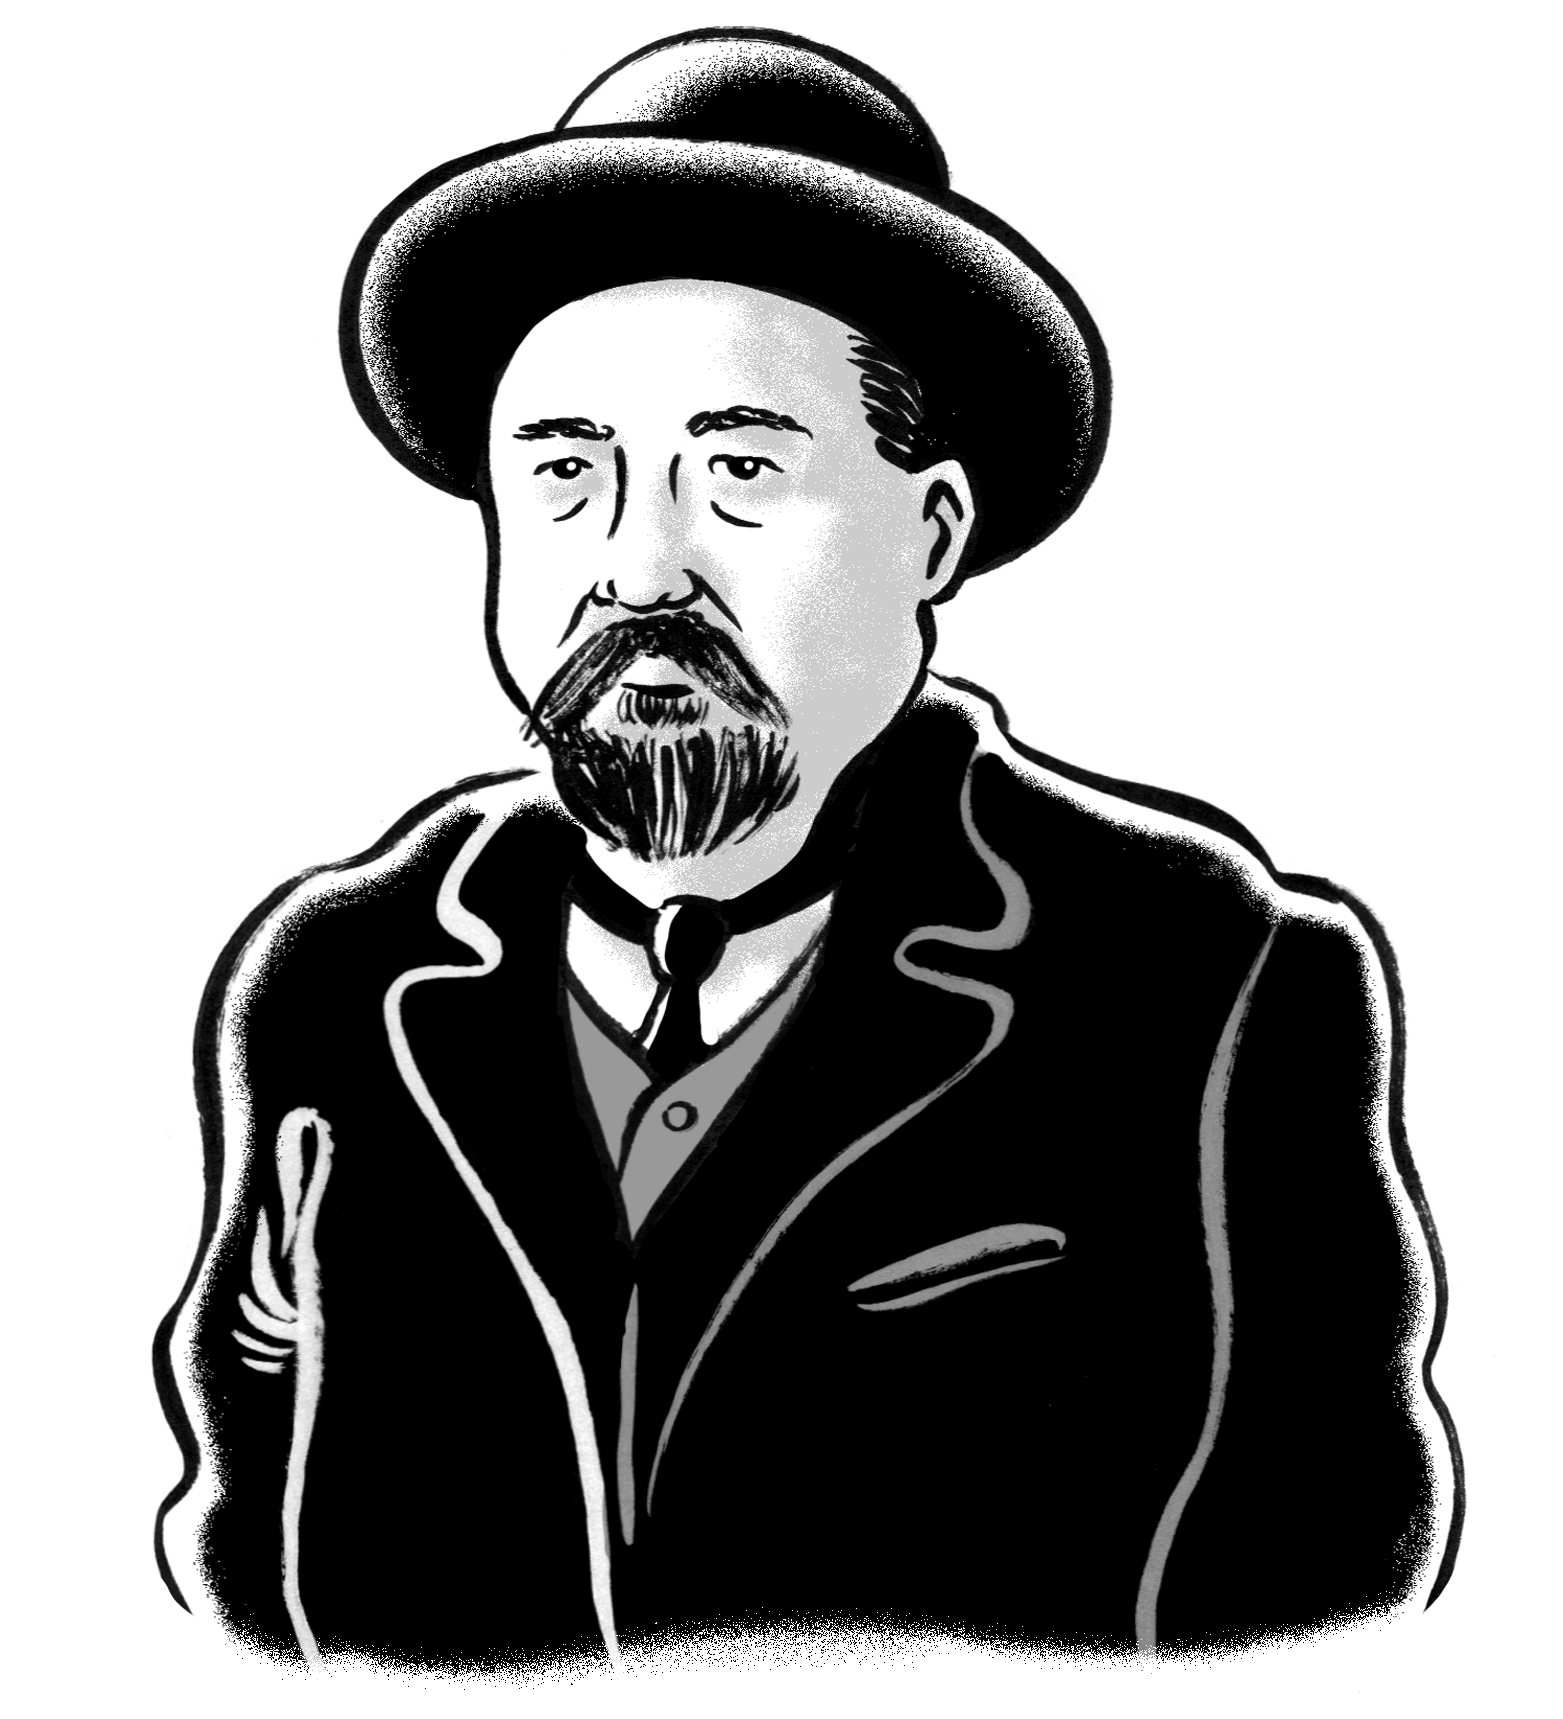
\includegraphics[width=6cm]{./imgs/autor9.jpg}
\end{center}

\chapter{O poodle branco}


\section{1}

\noindent{}Por veredas da costa montanhosa do Sul da Crimeia, vagava de povoado em
povoado uma pequena trupe itinerante. Geralmente à frente de todos
corria, com a língua cor"-de"-rosa pendurada no canto da boca, um
\emph{poodle} branco chamado Artô, tosado no estilo de um leão. Nos
cruzamentos, ele parava e, abanando o rabo, lançava um olhar
interrogativo para trás. Por sinais que apenas ele reconhecia, o cão
sempre sabia o caminho certo e, balançando alegremente as orelhas,
atirava"-se num galope para a frente. Atrás dele andava um menino de doze
anos, Serguei, que segurava, sob o braço esquerdo, um tapetinho para
exercícios de acrobacia e, na mão direita, uma gaiola com um pintassilgo
que havia sido ensinado a sacar bilhetinhos coloridos com leituras da
sorte. Na retaguarda, arrastava"-se o ancião da trupe, o vovô Martyn
Lodýjkin, com um realejo nas costas curvadas.

O realejo era velho, sofria de rouquidão e acessos de tosse, tendo
passado por mais de uma dezena de reparos durante a vida. Ele tocava
apenas duas músicas: uma triste valsa alemã de Launer e um
galope\footnote{Galope, música para dança húngara, de mesmo nome, com
  andamento rápido.} retirado de \emph{Viagem à China} --- ambas
sucessos de trinta ou quarenta anos atrás, tinham sido esquecidas por
todos havia tempo. Além disso, o realejo tinha dois tubos traiçoeiros. O
primeiro, para som agudo, perdera a voz e não tocava mais. Quando
chegava a vez dele, toda a melodia começava a engasgar, arrastar e
tropeçar. O outro tubo, que produzia som baixo, tinha uma válvula que
não fechava direito: ao ressoar uma nota baixa, o som continuava,
abafando todos os outros, até que de repente lhe dava vontade de se
calar. O vovô reconhecia todas as falhas de sua máquina e, de vez em
quando, comentava ironicamente e com uma pontinha de tristeza:

--- Fazer o quê?\ldots{} É um órgão velho\ldots{} Sujeito a resfriados\ldots{} Mal
começa a tocar, os moradores das \emph{datchas}\footnote{\emph{Datcha},
  propriedade rural com uma casa de veraneio e, a depender da área e das
  condições do dono, outras construções (casa de banho, casa de
  empregados, jardins, lagos, etc.).} se ofendem: ``Eca! Que
porcaria!''. Eram peças muito boas, da moda, só que o público de hoje em
dia não sabe apreciá"-las. Querem ouvir a \emph{Gueixa}, \emph{Sob a
águia de duas cabeças} ou a valsa do \emph{Vendedor de pássaros}. E tem
aquele probleminha nos tubos\ldots{} Levei para um especialista, nem quis
consertar. Falou que precisava colocar tubos novos\ldots{} ``O melhor seria'',
disse ele, ``vender essa tralha podre para um museu\ldots{} Que vire uma peça
de exposição\ldots{}'' Mas, deixe para lá! Ele nos alimentou até hoje,
Serguei, e, se Deus quiser, ainda nos alimentará.

O velho Martyn amava seu realejo como só se pode amar uma criatura viva,
alguém próximo ou um familiar. Acostumado a tê"-lo ao lado pelos longos
anos de vida árdua na estrada, começou a ver em seu instrumento um
companheiro com alma, quase consciente. Às vezes, de madrugada, durante
um pernoitar em alguma pousada barata e suja, o realejo, colocado no
chão junto à cabeceira de Martyn, de repente emitia um som baixo,
trêmulo, triste e solitário, como o suspiro de um velho. Então, Lodýjkin
acariciava o lado talhado do realejo sussurrando ternamente:

--- O que é que foi? Está gemendo, meu velho?\ldots{} Aguente firme\ldots{}

Da mesma forma que amava seu realejo --- ou talvez ainda mais ---,
Martyn amava os pequenos companheiros de estrada: o menino Serguei e o
\emph{poodle} Artô. O garoto ele tinha ``alugado'' uns cinco anos atrás
de um sapateiro viúvo e indolente, por dois rublos mensais. Mas logo o
sapateiro morreu e Serguei acabou ficando com o vovô Lodýjkin em
definitivo, tanto por laços de alma como por motivos de sobrevivência
diária.

\section{2}

A vereda contornava um alto penhasco na costa, volteando à sombra de
oliveiras centenárias. O mar às vezes surgia entre as árvores e, então,
parecia não apenas se estender ao longe, mas se elevar como uma poderosa
parede silenciosa, ficando mais azul, mais denso, nas aberturas
preenchidas por uma folhagem verde"-prateada. Na relva, nos arbustos de
corniso e de rosas silvestres, nas vinhas e nas árvores, em todo lugar
penetrava o canto das cigarras, fazendo o ar tremular nesse zunido
monótono e incessante. O dia estava muito quente, sem vento, e as solas
dos pés queimavam sobre a terra aquecida.

Serguei, andando, como de hábito, à frente do vovô, volta e meia
diminuía o passo e aguardava o velho o alcançar.

--- Que foi, Serioja?\footnote{Serioja, apelido de Serguei.} --- indagou
o tocador de realejo.

--- Está muito quente, vovô Lodýjkin\ldots{} Não dá para aguentar! Se
déssemos um mergulho\ldots{}

O velho Martyn, sempre andando, corrigiu o realejo nas costas com um
movimento costumeiro do ombro e secou com a manga a face suada.

--- Não seria nada mal! --- suspirou ele, olhando com vontade para a
superfície azul e refrescante do mar. --- Só que, depois de nos
banharmos, sentiríamos mais moleza. Um médico conhecido me contou que
esse sal exerce um tipo de ação na gente\ldots{} Isto é, a pessoa fica como
que relaxada\ldots{} Pois é sal marinho\ldots{}

--- Talvez ele mentisse? --- observou Serguei, desconfiado.

--- Ora essa! Por que ele iria mentir? Era um homem decente, não
bebia\ldots{} Tinha uma casinha em Sebastopol. E daqui não conseguimos descer
até o mar. Espere um pouco, logo chegaremos a Miskhоr e ali lavaremos
nossas pobres carcaças. É agradável se banhar antes do almoço\ldots{} E
depois tirar um cochilo\ldots{} Que coisa boa\ldots{}

Artô, que ouvia a conversa atrás de si, virou"-se e correu na direção
deles. Seus bondosos olhos azuis estavam semicerrados de calor, e a
língua comprida, puxada para fora, tremia por causa da respiração
acelerada.

--- Então, meu amigo canino, está quente, não é? --- perguntou o velho.

O cão deu um bocejo tenso, enrolando a língua em um tubinho, sacudiu o
corpo e ganiu com voz fina.

--- Pois é, amiguinho, não há o que fazer\ldots{} Está escrito no suor do seu
rosto\ldots{} --- continuava Lodýjkin em tom professoral. --- A bem da
verdade, você não tem um rosto, mas um focinho, em todo caso\ldots{} Vá, siga
em frente, não fique no meio do caminho\ldots{} Sabe, Serioja, devo admitir
que gosto quando está assim tão quente. Só o órgão atrapalha um pouco,
mas, se não fosse pelo trabalho, eu me deitaria em um lugarzinho na
grama, na sombra, com a barriga para cima, e ficaria esticado um
tempo\ldots{} Para nossos velhos ossos não há coisa melhor do que este sol.

A trilha descia juntando"-se а uma estrada larga de um branco ofuscante,
dura feito pedra. Ali começava o antigo parque de um conde, em cuja
vegetação abundante se estendiam bonitas \emph{datchas} com chafarizes,
canteiros e estufas de flores. Lodýjkin conhecia bem aquela região; todo
ano ele peregrinava lá, indo de um local a outro, durante a época das
uvas, quando a Crimeia se enchia de um público abastado e alegre. O
esplendor da natureza do sul não tocava mais o velho, em compensação
deixava admirado Serguei, que estava ali pela primeira vez. As magnólias
de folhas grossas e brilhantes, parecendo envernizadas, com flores
brancas do tamanho de um prato; os caramanchões cobertos por pesados
cachos de uva pendentes; os enormes plátanos centenários com troncos
claros e copas majestosas; as plantações de tabaco, os riachos e as
cachoeiras; as rosas imponentes, magníficas e perfumadas que cresciam em
toda parte, nos canteiros, nas sebes e nas paredes das \emph{datchas}
--- toda essa beleza viva e florida não parava de surpreender a alma
sensível e ingênua do menino. Ele expressava sua admiração em voz alta,
puxando a manga do velho a cada minuto:

--- Vovô Lodýjkin, olhe só! Ali, no chafariz\ldots{} Peixes dourados!
Palavra, vovô, são dourados mesmo, coisa inacreditável! --- gritava o
garoto, encostando o rosto na grade de um jardim com uma grande piscina
no meio. --- Olhe, vovô, pêssegos! São tantos! E todos numa árvore!

--- Ande, ande, bobinho, não pare aí de boca aberta! --- o velho sorria,
empurrando"-o de leve. --- Espere até chegarmos à cidade de Novorossiisk,
ou seja, até irmos de novo para o sul. Ali há lugares em que vale
realmente passar a vista. Você verá, por exemplo, Sótchi, Ádler, Tuapsé
e, depois, meu caro, ainda Sukhum e Batum\ldots{} É de encher os olhos\ldots{} Tem
lá, por exemplo, tal palmeira. Impressionante! O tronco aveludado, como
que feito de feltro, e cada folha é tão grande, que embaixo dela
poderíamos nos abrigar.

--- Jura?! --- surpreendia"-se Serguei, animado.

--- Você mesmo verá. Ih, quer mais? Há laranjas e até limões, por
exemplo\ldots{} Já os viu nas mercearias?

--- Sim\ldots{}

--- Pois é, crescem à vontade. Sem nada além de ar, dão nas árvores, são
como as maçãs e as peras para nós\ldots{} E o povo lá, meu caro, é singular:
turcos, persas, todo tipo de circassianos, todos de cafetãs e adagas na
cintura\ldots{} Е são cabeça quente! E ainda, meu caro, os etíopes. Eu os vi
diversas vezes em Batum.

--- Etíopes? Estes eu conheço. Aqueles com chifres --- disse Serguei,
convicto.

--- Chifres, a bem da verdade, eles não têm, isso é mentira. Eles têm a
pele negra e brilhante como uma bota lustrada. Lábios carnudos e
vermelhos, olhos brancos e cabelos encaracolados, como os pelos pretos
de um carneiro.

--- Dão medo\ldots{} os etíopes?

--- Como dizer? Por falta de hábito, no início você sente algum
receio\ldots{} Depois você percebe que os outros não se importam e isso o
encoraja\ldots{} Sim, meu querido, há muita variedade por lá. Quando
chegarmos, você mesmo verá. A única coisa ruim é a malária. Ao redor há
pântanos e brejos sujos, e um calor infernal. Para os locais nada disso faz mal, mas para as pessoas de fora é um sofrimento e tanto. Mas,
meu amigo, chega de conversa fiada. Passe por baixo desse portão. Nessa
\emph{datcha} vivem senhores muito bons. Pode crer! Eu sei das coisas!

Nesse dia, porém, eles não tiveram sorte. De uns lugares foram expulsos
de longe; em outros, às primeiras notas roucas e roufenhas do realejo,
responderam dos terraços com gestos impacientes e irritados; em alguns,
os empregados comunicaram que os senhores ainda não tinham chegado. Em
duas \emph{datchas}, é verdade, eles conseguiram receber pela
apresentação, mas muito pouco. O velho, porém, não desdenhava de ganhos
miúdos. Saindo dos portões na direção da estrada, ele, com ar
satisfeito, chacoalhava as moedinhas no bolso dizendo bondosamente:

--- Dois e cinco dão sete copeques\ldots{} Pois bem, Serioja, isso também é
dinheiro. Sete vezes sete dão quase cinquenta; isso significa que nós
três seremos bem alimentados e teremos um lugar para pernoitar, e o
velho Lodýjkin, por sua fraqueza е grande esforço, terá direito a um
pequeno cálice\ldots{} Pois é, os patrões não compreendem isso! Dar uma moeda
de cinco consideram vergonhoso e dar uma de vinte um desperdício\ldots{}
Então mandam você embora. Que sejam três copeques, são mais que nada\ldots{}
Eu não me ofendo, por mim tudo bem\ldots{} Por que é que eu me ofenderia?

Em geral, Lodýjkin era um homem de temperamento pacato e, mesmo quando
era expulso dos lugares, não se queixava. Mas, nesse dia, ele foi tirado
de seu habitual estado de serenidade por uma senhora simpática e
rechonchuda que, à primeira vista, parecia generosa. Era proprietária de
uma linda \emph{datcha} cercada por um jardim cheio de flores. Ela
escutou a música com atenção e viu, ainda mais atenta, os números
acrobáticos de Serguei e os truques engraçados de Artô. Depois da
apresentação, demoradamente conversou com o garoto, perguntando quantos
anos tinha, como se chamava, onde havia aprendido ginástica, qual era o
parentesco com o velho, quem eram seus pais, etc. Então mandou"-os
aguardar do lado de fora e saiu da sala.

Passaram dez minutos, depois quinze, e ela não aparecia, e, quanto mais
tempo passava, mais cresciam as expectativas indefinidas e sedutoras dos
artistas. O velho até sussurrou no ouvido do menino, encobrindo
cautelosamente a boca com a palma da mão:

--- Escute, Serioja, demos sorte, eu sei das coisas. Na certa, ela dará
uma peça de roupa ou um par de calçados. Pode crer!\ldots{}

Finalmente a dona apareceu no terraço, jogou de cima uma moedinha
prateada na cartola esticada por Serguei e imediatamente se retirou. Era
uma moeda velha e gasta de dez copeques e, ainda por cima, furada no
meio. O velho longamente a observou, atônito. Já andando pela estrada,
bem longe da propriedade, ele ainda segurava a moedinha na mão, como se
a pesasse.

--- Hu"-u"-u"-m\ldots{} Bem feito! --- proferiu ele repentinamente, detendo"-se.
--- Que resta dizer?\ldots{} Nós, três paspalhos, nos empenhamos para valer!
O melhor seria nos jogar um botão. Este, pelo menos, serviria para
prender em algo. E o que vou fazer com esta porcaria? A madame deve
pensar: ah, aquele velhote de qualquer jeito usará a moeda com alguém de
madrugada, no escuro. Pois está muito enganada, dona, o velho Lodýjkin
não faz essas indecências! Tome seus preciosos vinténs! Lá vai!

Cheio de indignação e orgulho, o velho arremessou ao chão a moeda, que
tilintou baixinho e afundou na poeira branca da estrada.

Assim, o velho, o menino e o cão percorreram uma localidade inteira de
\emph{datchas}, indo pelo caminho do mar. À frente deles, do lado
esquerdo da estrada, encontrava"-se a última. O casarão escondiа-se atrás
de um muro alto e branco, ao longo do qual sobressaía uma densa fileira
de ciprestes finos e empoeirados, lembrando fusos pontiagudos e
enegrecidos. Só chegando perto dos portões de ferro com um trançado
esmerado, podia"-se ver um canto do gramado fresco e sedoso, de um verde
vivo, com canteiros arredondados e, no fundo, uma aleia de passagem
coberta com uvas silvestres. No meio do gramado, o jardineiro regava as
rosas com uma mangueira comprida. Ele tampou a extremidade do cano com o
dedo e, sob o sol, respingos jorravam em forma de chafariz, refletindo
todas as cores do arco"-íris.

O vovô Lodýjkin ia passar direto, mas, ao olhar pelo portão, parou,
atônito.

--- Espere um pouco, Serioja --- chamou ele. --- Não é que tem gente se
mexendo ali? Ora essa! Tantos anos andando nos arredores e nunca vi uma
alma viva dentro. Vamos, companheiro!

--- ``Vila da Amizade, a entrada de estranhos é estritamente proibida''
--- o menino leu a placa talhada com arte num dos postes que escoravam o
portão.

--- ``Amizade''?\ldots{} --- repetiu o velho analfabeto. --- Isso mesmo! É a
palavra mais verdadeira, a amizade. O dia todo a coisa empacou para o
nosso lado, agora pegaremos o que nos cabe. Pode crer, eu farejo isso
feito um cão de caça. Artô, \emph{ici},\footnote{\emph{Ici}, do francês:
  ``aqui''.} filho de uma cachorra! Entre, Serioja, seja corajoso.
Sempre me dê ouvidos, eu sei das coisas!

\section{3}

As sendas do jardim estavam cobertas com cascalho graúdo, que farfalhava
sob os pés, e decoradas, nas laterais, com grandes conchas cor"-de"-rosa.
Nos canteiros, sobre uma relva variegada de ervas multicolores, surgiam
flores exóticas exalando um aroma doce no ar. A água cristalina
murmurava ao borrifar em lagos artificiais; guirlandas de folhas
entrelaçadas caíam de lindos vasos suspensos no ar entre as árvores. A
entrada da casa era emoldurada com pilares de mármore, onde havia duas
esferas espelhadas em cima, nelas os saltimbancos se refletiram de
cabeça para baixo, em uma imagem engraçada, toda alongada e contorcida.

Na frente do terraço, havia um grande pátio de terra batida. Serguei
estendeu ali seu tapetinho, e o velho, que havia apoiado o realejo num
bastão, estava prestes a girar a manivela quando uma cena inesperada e
estranha desviou sua atenção.

Um menino entre oito e dez anos, saindo de um dos quartos, lançou"-se no
terraço feito um projétil, gritando com voz estridente. Vestia uma
roupinha de marinheiro que deixava seus braços e joelhos à mostra. Seus
cabelos louros e cacheados caíam desordenadamente nos ombros. Atrás dele
saíram correndo seis pessoas: duas empregadas de aventais; um velho e
gordo mordomo de fraque, sem barba e sem bigodes, mas com costeletas
longas e grisalhas; uma moça magricela de cabelos ruivos e nariz
vermelho com um vestido xadrez azul; uma jovem senhora de aspecto
doentio, mas muito bonita, usando um penhoar azul"-claro de renda; e,
finalmente, um senhor careca e rechonchudo, de terno de seda e óculos
dourados. Todos pareciam muito nervosos, gesticulavam, falavam alto e
até se empurravam. Não era difícil adivinhar que o motivo das
preocupações era o menino de roupa de marinheiro que tão repentinamente
surgiu no terraço.

Enquanto isso, o culpado de todo o alvoroço, sem parar nem por um
segundo de gritar, atirou"-se de bruços no chão de pedra, virou rápido de
costas e começou furiosamente a agitar os braços e as pernas. Os adultos
о rodearam, aflitos. O velho mordomo de fraque, encostando com ar de
súplica as mãos no peito de camisa engomada, disse queixosamente,
balançando as costeletas:

--- Meu caro senhor! Nikolai Apollónovitch!\ldots{} Por favor, não dê esse
desgosto a sua mãe, levante"-se\ldots{} Seja bonzinho, tome o remédio. O
xarope é muito doce, uma calda de açúcar! Faça o favor, levante"-se\ldots{}

As criadas de aventais lançavam os braços para o alto е chilreavam com
vozes servis e assustadas. A moça de nariz vermelho gesticulava
dramaticamente gritando algo importante, mas de todo incompreensível, decerto em língua estrangeira. O senhor de óculos
dourados persuadia o menino em tom ponderado, inclinando a cabeça de um
lado para outro e conduzindo as mãos com gravidade. E a jovem senhora
gemia languidamente, pressionando um lenço de renda no canto dos olhos:

--- Oh, Trilly, ah, meu Deus!\ldots{} Meu anjo, eu imploro. Escute, a sua mãe
está implorando a você. Por favor, tome já, tome seu remédio. Você verá
que ficará bom num instante: a barriguinha parará de doer e a cabeça
também. Faça isso por mim, meu docinho! Pois bem, quer que a mamãe fique
de joelhos, não é?\ldots{} Olhe, estou de joelhos na sua frente. Quer uma
moedinha de ouro? Duas? Cinco moedinhas, hem, Trilly? Quer um burrinho
de verdade? Quem sabe um cavalinho?\ldots{} Fale alguma coisa para ele,
doutor!\ldots{}

--- Escute, Trilly, seja homem, afinal --- falou em tom grave o senhor
de óculos dourados.

--- Ai"-ai"-aaai! --- berrava o menino, contorcendo"-se pelo terraço e
esperneando com desespero.

Apesar de sua extrema agitação, ele não perdia a chance de chutar com as
botas as barrigas e as pernas das pessoas ao seu redor, as quais, aliás,
conseguiam se desviar com bastante habilidade.

Serguei, que havia tempo observava curioso e espantado essa cena,
cutucou de leve seu velho companheiro.

--- Vovô Lodýjkin, o que há com ele? --- perguntou baixinho. --- Será
que iam lhe dar uma surra?

--- Imagine, uma surra\ldots{} Ele mesmo é capaz de surrar qualquer um. É
apenas um menino sem juízo. Talvez doente.

--- Possuído? --- tentou adivinhar Serguei.

--- E eu vou lá saber? Fale baixo!\ldots{}

--- Ai"-ai"-ai! Inúteis! Idi"-o"-tas!\ldots{} --- o garoto gritava cada vez mais
alto.

--- Comece o número, Serguei. Sei o que estou fazendo! --- mandou de
repente Lodýjkin e, com ar decidido, girou a manivela do realejo.

Os sons roufenhos e dissonantes do antigo galope invadiram o jardim.
Todos da varanda estremeceram ao mesmo tempo, até o menino se calou por
um instante.

--- Ah, meu Deus, eles irão deixar o pobre Trilly ainda mais abalado!
--- exclamou a madame chorosa de penhoar azul"-claro. --- Mandem"-nos
embora daqui, rápido! E ainda esse cão sujo com eles. Os cachorros
trazem doenças horríveis. Não fique parado como uma estátua, Ivan! ---
com expressão cansada e de repugnância, ela abanou o lenço na direção
dos artistas.

A magrela de nariz vermelho arregalou os olhos de raiva, alguém começou
a resmungar em tom de ameaça\ldots{} O homem de fraque, em passos apressados
e suaves, desceu do terraço e, com uma expressão de pavor no rosto,
abrindo os braços para os lados, correu na direção do tocador de
realejo.

--- Que pouca"-vergonha! --- disse em um sussurro sufocado e assustado,
mas ao mesmo tempo autoritário e sério. --- Com que permissão? Quem os
deixou entrar? Andem! Fora daqui!\ldots{}

O realejo deu um pio desanimado e silenciou.

--- Meu caro senhor, permita"-me explicar\ldots{} --- começou delicadamente o
velho.

--- Nada disso! Fora! --- gritou o mordomo, e da voz dele saiu um leve
assobio.

Seu rosto gordo instantaneamente enrubesceu, enquanto os olhos
arregalaram, quase saltando das órbitas, e começaram a se agitar. A
imagem era tão amedrontadora, que Lodýjkin involuntariamente deu dois
passos para trás.

--- Arrume as coisas, Serguei --- disse ele colocando apressadamente o
realejo nas costas. --- Vamos embora!

Nem deram dez passos, soaram do terraço novos gritos estridentes:

--- Ai"-ai"-ai! Quero! De"-e"-ê! Para mim! Ah"-ah"-ah! Chame!

--- Mas, Trilly!\ldots{} Oh, meu Deus, Trilly! Ah, chamem"-nos de volta ---
gemeu a dona, nervosa. --- Ah, como vocês são desajeitados!\ldots{} Ivan,
está me ouvindo? Chame aqueles mendigos agora!\ldots{}

--- Escutem! Ei, vocês! Tocador de realejo! Voltem! --- gritaram várias
vozes do terraço.

O mordomo gordo, com as costeletas voando para os lados, saltou feito
uma bola de borracha na direção dos artistas, que estavam partindo.

--- Não!\ldots{} Ei, músicos! Escutem! Parem! Voltem!\ldots{} --- gritava ele,
ofegante, abanando os braços. --- Meu velho --- ele finalmente agarrou
Lodýjkin pela manga ---, dê meia"-volta! Os senhores irão ver a pantomima
de vocês. Depressa!\ldots{}

--- Ora essa! --- suspirou o velho, meneando a cabeça, mas se aproximou
do terraço, tirou o realejo, firmando"-o a sua frente sobre o bastão, e
continuou a tocar o galope do ponto em que fora interrompido havia
pouco.

A agitação na varanda se acalmou. A senhora, o menino e o homem de
óculos dourados se aproximaram da balaustrada, os demais respeitosamente
permaneceram no fundo. De dentro do jardim veio o jardineiro de avental
e se posicionou perto de Lodýjkin. Atrás do jardineiro, postou"-se o
caseiro vindo de algum canto. Era um sujeito enorme e barbudo, com a
testa estreita e o rosto bexiguento do qual não desparecia uma expressão
sombria. Ele vestia uma camisa nova cor"-de"-rosa com bolinhas pretas
dispostas na diagonal.

Sob o som rouco e engasgado do galope, Serguei esticou seu tapetinho no
solo, rapidamente tirou as calças de lona (elas tinham sido feitas de
saco velho e atrás, na parte mais larga, aparecia a marca retangular do
fabricante), tirou a jaqueta gasta e ficou de um velho macaquinho de
tricô que, apesar das várias remendas, caía perfeitamente em seu corpo
forte, flexível e gracioso. Ele já tinha aprendido, imitando ginastas
adultos, as técnicas de um verdadeiro acrobata. Enquanto subia no
tapete, levou as mãos aos lábios e, num gesto teatral, abriu os braços
para os lados, mandando com esse movimento dois beijos ardentes ao
público.

Com uma mão, Lodýjkin girava ininterruptamente a manivela do realejo,
que produzia uma melodia trêmula e tossida; com a outra mão, arremessava
ao menino diversos objetos, que ele, com destreza, pegava no ar. O
repertório de Serguei era pequeno, mas seu trabalho era bom, ``limpo'',
como diziam os acrobatas, e executado com vontade. O garoto jogou para o
alto uma garrafa vazia de cerveja, que girou algumas vezes no ar, aí ele
a apanhou pelo gargalo com a borda de um prato, equilibrando"-a assim por
alguns segundos; fez malabarismo com quatro bolas de marfim e também com
duas velas, que caíram ao mesmo tempo em castiçais; depois lançou para
cima três objetos diferentes: um leque, um charuto de madeira e uma
sombrinha. Os três voavam pelo ar, sem tocar o chão, e, de repente, a
sombrinha estava parada sobre a cabeça dele, o charuto metido na sua
boca, e o leque abanando seu rosto de maneira sedutora. No encerramento,
Serguei deu algumas cambalhotas no tapete, fez a posição do ``sapo'',
demonstrou o ``nó americano'' e andou sobre as mãos. Ao esgotar sua
reserva de truques, ele novamente lançou dois beijos ao público e,
ofegante, foi até o vovô para substituí"-lo no realejo.

Agora era a vez do Artô. O cão sabia bem disso e fazia tempo que pulava
ansiosamente com as quatro patas sobre Lodýjkin, latindo de maneira
entrecortada e nervosa ao dono, o qual tentava se livrar, pelo lado, da
alça do realejo. Quem sabe o \emph{poodle} sabichão quisesse dizer com
isso que, na sua opinião, não era prudente praticar exercícios
acrobáticos quando fazia mais de vinte e sete graus na sombra? Mas
Lodýjin, com olhar ladino, puxou das costas uma vareta de corniso. ``Eu
sabia!'', o cão com ar descontente deu um último latido e, preguiçoso e
contrariado, ergueu"-se nas patas traseiras, sem tirar os olhos piscantes
do dono.

--- De pé, Artô! Isso, isso, isso mesmo\ldots{} --- dizia o velho, mantendo a
vareta sobre a cabeça do animal. --- Agora vire ao contrário, mais, mais
um pouco\ldots{} Dance, cachorrinho, dance! Sente! O quê? Não quer? Eu disse
sentado! Ã"-hã\ldots{} Muito bem! Obedeça, cachorrinho! Agora cumprimente o
respeitável público! Artô! --- Lodýjkin levantou a voz em tom de ameaça.

``Au!'', soltou o \emph{poodle} com desprezo. Depois, piscando queixosamente,
ergueu os olhos para o dono e acrescentou duas vezes: ``Au, au!''.

``Não, meu velho não me compreende!'', escutava"-se em seu latido
inconformado.

--- Ah, bom, assim está melhor! A cortesia antes de tudo. Agora, vamos
pular um pouco --- continuava o velho, esticando a vareta perto do solo.
--- Avante! Não precisa mostrar a língua, amigo. Avante! Upa! Magnífico!
Mais uma vez, \emph{noch einmal}\ldots{}\footnote{\emph{Noch einmal,} do
  alemão: ``mais uma vez''.} Avante!\ldots{} Upa! Avante! Upa! Magnífico,
cachorrinho! Quando voltarmos para casa, ganhará uma cenourinha. Ah,
você não come cenoura? Esqueci completamente. Então pegue a minha
cartola e peça aos senhores. Quem sabe eles te concedam algo mais
apetitoso.

Lodýjkin fez com que o cachorro levantasse sobre as patas de trás e
enfiou em sua boca um velho quepe ensebado, que ele muito
espirituosamente chamava de ``cartola''. Segurando o quepe com os dentes
e derreando nas patas traseiras flexionadas, Artô se aproximou do
terraço. Nas mãos da mulher de aspecto doentio surgiu um pequeno
porta"-moedas de madrepérola. Todos ao redor sorriam com compaixão.

--- Viu? Eu não disse? --- com entusiasmo sussurrou o velho,
inclinando"-se a Serguei. --- Sempre me dê ouvidos, companheiro, eu sei
das coisas. Não será menos de um rublo.

Nesse momento, do terraço soou um grito tão agudo e desesperado, quase
desumano, que Artô, desamparado, deixou cair o quepe da boca e, pulando
com o rabo entre as pernas, olhando para trás com medo, atirou"-se aos
pés do dono.

--- Que"-e"-ro! --- gritava o menino de cachos, batendo os pés. --- Para
mim! Quero! O ca"-a"-chorro! Trilly
quer o cachorro"-o"-o!

--- Ah, meu Deus! Ah! Nikolai Apollónovitch!\ldots{} Meu bom senhor!\ldots{}
Acalme"-se, Trilly, imploro a você! --- novamente começou o alvoroço no
terraço.

--- Ca"-a"-chorro! Deem o cachorro! Quero o cachorro! Inúteis, diabos,
idiotas! --- o menino estava fora de si.

--- Mas, meu anjo, não se torture assim! --- balbuciava a dama de
penhoar azul. --- Você quer fazer um carinho no cachorro? Tudo bem, tudo
bem, meu amor, agora mesmo. Doutor, o que o senhor acha, Trilly pode
acariciar esse cachorro?

--- Em geral, eu não aconselharia --- ele fez um gesto vago afastando as
mãos ---, mas, se houver desinfecção, digamos, com ácido bórico ou uma
solução diluída de fenol, então\ldots{} Em geral\ldots{}

--- Ca"-a"-chorro!

--- Um momentinho, meu amor, um momentinho. Pois bem, doutor, mandaremos
lavar o cão com ácido bórico, então\ldots{} Ah, Trilly, por favor, não se
desespere assim! Faça o favor, velho, traga o cachorro para cá. Não se
preocupe, o senhor será pago. Escute, ele tem alguma doença? Quer dizer,
ele tem raiva? Ou talvez o verme da equinococose?

--- Não quero fazer carinho, não quero! --- gritava Trilly, espumando de
raiva. --- Quero para sempre! Diabos, imbecis! Todo meu! Quero brincar
eu mesmo\ldots{} Para sempre!

--- Escute, velho, chegue mais perto --- a madame tentava falar mais
alto do que o filho. --- Ah, Trilly, você ainda me mata com esses
gritos. Ah, para que, meu Deus, deixaram esses músicos entrarem aqui?!
Chegue mais perto, por Deus, mais\ldots{} Eu disse mais perto! Assim\ldots{} Ah,
não fique tão aflito, Trilly, mamãe fará qualquer coisa por você. Mas
imploro\ldots{} \emph{Miss}! Acalme a criança, afinal\ldots{} Doutor, por favor\ldots{}
Quanto você quer, velho?

Lodýjkin tirou o quepe. Seu rosto ganhou uma expressão cortês e
sofredora.

--- Quanto a dona desejar, senhora, Excelência\ldots{}. Somos gente simples,
para nós qualquer doação é uma bênção\ldots{} Creio que a senhora não
ofenderia um velho\ldots{}

--- Ah, como o senhor é confuso! Trilly, ficará com a garganta dodói.
Compreenda, o cachorro é \emph{seu}, e não meu. Então, quanto? Dez?
Quinze? Vinte?

--- Ah"-ah"-ah! Eu que"-e"-ro! Dê o cachorro, dê o cachorro --- o menino se
esgoelava e chutava a barriga redonda do mordomo.

--- Quer dizer\ldots{} perdoe, Excelência --- Lodýjkin dissimulou. --- Sou um
homem velho e tolo\ldots{} Não entendo tudo de uma vez\ldots{} Também sou meio
surdo\ldots{} O que a senhora disse?\ldots{} Pelo cão?

--- Ah, meu Deus!\ldots{} O senhor quer se fazer de idiota? --- a mulher
ficou irritada. --- Babá, traga um pouco de água para Trilly, depressa!
Eu estou falando na mesma língua do senhor: por quanto você venderia seu
cachorro? O senhor entende, o cachorro, o seu cachorro\ldots{}

--- Cachorro! Cachorro! --- gritava o menino, mais estridente.

Lodýjkin, ofendido, colocou o quepe na cabeça.

--- Não vendo cachorros, madame --- proferiu friamente e com dignidade.
--- E este cão, minha senhora, a bem da verdade, a nós dois --- ele
apontou com o dedão para Serguei ---, a nós dois ele alimenta, veste e
sustenta. E não se pode, de maneira alguma, fazer uma coisa dessas, quer
dizer, vendê"-lo.

Nesse momento, a voz de Trilly atingiu a altura de um silvo de
locomotiva. Deram"-lhe um copo de água, mas ele o lançou com raiva no
rosto da governanta.

--- Escute, velho insano! Não existe coisa que não possa ser vendida ---
insistia a dona pressionando as têmporas com as mãos. --- \emph{Miss},
enxugue logo o rosto e traga o meu remédio para enxaqueca. Talvez o seu
cão custe cem rublos? Ou duzentos? Trezentos? Responda, sua estátua!
Doutor, pelo amor de Deus, diga alguma coisa para ele!

--- Arrume as suas coisas, Serguei --- resmungou Lodýjkin, taciturno.
--- Es"-tá"-tua\ldots{} Artô, venha cá!\ldots{}

--- Espere aí, meu caro --- o homem gordo de óculos dourados falou de
modo arrastado e autoritário. --- É melhor você não se fazer de difícil,
meu caro, eis o que tenho a dizer: seu cachorro não vale mais de dez
rublos, e este preço inclui a sua parte\ldots{} Pense bem no que estão lhe
oferecendo, trouxa!

--- Muito agradecido, caro senhor, é que\ldots{} --- Lodýjkin, gemendo de
dor, pôs o realejo de volta nos ombros ---, é que não há como fazer esse
negócio, quer dizer, vender. Melhor os senhores procurarem outro
cãozinho por aí\ldots{} Passem bem\ldots{} Serguei, vá andando!

--- Cadê o seu passaporte? --- de repente o doutor levantou a voz, em
tom de ameaça. --- Conheço canalhas como você!

--- Caseiro! Semion! Mande"-os embora! --- gritou a dama com o rosto
distorcido de raiva.

O caseiro sombrio de camisa cor"-de"-rosa aproximou"-se com aspecto
sinistro dos artistas. Enquanto isso, no terraço se levantou uma
gritaria terrível de diferentes vozes: Trilly berrava, fora de si; sua
mãe dava gemidos; a babá e sua ajudante diziam lamentos ligeiros e
repetitivos; o médico, parecendo um zangão irritado, zunia num baixo
encorpado. Mas vovô Lodýjkin e Serguei não ficaram tempo suficiente para
ver o desfecho da cena. Precedidos pelo assustado \emph{poodle}, eles
praticamente correram até os portões. Atrás deles vinha o caseiro,
empurrando o realejo e falando em voz ameaçadora:

--- Ficam de vadiagem por aí, vigaristas! Agradeça a Deus, matusalém,
por não terem levado uma surra. Na próxima vez que aparecerem aqui,
saiba que não vou me segurar, apanharei pelo cangote e levarei para a
polícia. Imprestáveis!

Por longo tempo o velho e o garoto andaram em silêncio, mas, de
repente, como se tivessem combinando, trocaram olhares e caíram na
risada: primeiro, Serguei e, em seguida, olhando para o menino, o
próprio Lodýjkin, embora este risse com certo constrangimento.

--- Então, vovô Lodýjkin? Você sabe das coisas, hem? --- provocava"-o
Serguei com malícia.

--- Pois é, companheiro. Fomos enganados --- o velho balançou a cabeça.
--- Mas que menininho virulento é aquele\ldots{} E como é que o educaram
assim, puxa vida? Haja paciência: vinte e cinco pessoas ficam dançando
ao redor dele. Fosse meu, eu lhe mostraria o que é bom para a tosse!
Deem o cachorro, dizia\ldots{} Como pode? Se amanhã ele quiser a Lua do céu,
lhe darão a Lua? Venha cá, Artô, meu cachorrinho. Que dia\ldots{} É
impressionante!

--- Não poderia ter sido melhor! --- Serguei continuava a zombar dele.
--- Uma madame deu uma peça de roupa, outra um rublo inteiro. Você, vovô
Lodýjkin, sabe mesmo prever o futuro.

--- E você fique quieto, toco de gente --- retrucou o velho sem raiva.
--- Lembra como fugiu do caseiro? Pensei que eu não alcançaria você. Um
homem sério é aquele caseiro.

Saindo do parque, os saltimbancos desceram por uma trilha íngreme e
escorregadia até o mar. Ali, as montanhas se recolheram um pouco, dando
espaço a uma faixa estreita de pedras, as quais haviam sido polidas pela
ressaca e, agora, eram delicadamente banhadas pelo mar, que sussurrava
sem alarde. A umas duzentas braças da costa, delfins davam saltos na
água, mostrando por um instante suas costas oleosas e arredondadas. Ao
longe, no horizonte, onde a superfície sedosa azul"-clara do mar era
circundada por uma borda aveludada azul"-escura, erguiam"-se as velas
esbeltas e rosadas de sol dos barcos de pesca.

--- É aí que vamos nos banhar, vovô Lodýjkin --- decidido, disse
Serguei, que já tinha tirado suas calças no caminho, ora pulando num pé,
ora no outro. --- Deixe"-me ajudar a tirar o órgão.

O menino rapidamente se livrou do resto da roupa, bateu sonoramente as
palmas no corpo bronzeado, cor de chocolate, e se jogou na água,
levantando ao redor muita espuma borbulhante.

O velho se despia sem pressa. Protegendo os olhos semicerrados do sol
com a palma da mão, ele observava Serguei e sorria com ternura.

``Quem diria, o rapazinho está crescendo'', pensava Lodýjkin, ``embora
seja só pele e osso, será um jovem forte.''

--- Ei, Serioja! Não vá muito longe. O porco"-do"-mar pegará você.

--- Eu é que о pegarei pelo rabo! --- gritou o menino de longe.

O velho ficou muito tempo sob o sol, apalpando volta e meia debaixo dos
braços. Para a água ele foi com muito cuidado e, antes de mergulhar,
molhou aplicadamente a calva vermelha e os flancos magros. Seu corpo
amarelo era flácido e fraco; as pernas incrivelmente finas; as costas,
com escápulas acentuadas, curvaram"-se depois dos longos anos carregando
o realejo.

--- Vovô Lodýjkin, olhe! --- gritou Serguei.

Ele deu uma cambalhota na água, jogando as pernas por cima da cabeça.

O velho, que estava agachado com água até a cintura e gemia de
satisfação, gritou preocupado:

--- Ei, nada de brincadeiras, porquinho! Cuidado!

Artô latia freneticamente e dava pulos na beira do mar. Afligia"-se por
Serguei ter se afastado muito. ``Para que se fazer de valente?'',
agitava"-se o \emph{poodle}. ``Há terra o suficiente para se andar. É
melhor assim.''

Ele próprio tinha entrado no mar até a barriga encostar na água, dando
algumas lambidas para experimentá"-la. Mas a água salgada não o agradou e
as ondas leves que rumorejavam sobre o cascalho o assustavam. O cão
pulou para a margem e pôs"-se a latir para Serguei de novo. ``Para que
esses truques bobos? Por que não ficar sentado na beira do mar ao lado
do velho? Ah, quantas preocupações me dá esse menino!''

--- Ei, Serioja, saia daí, já chega, de verdade! --- chamou o velho.

--- Estou indo, vovô Lodýjkin --- respondeu o menino. --- Vou de navio:
U"-u"-u"-u"-u!

Ele finalmente nadou até a margem, mas, antes de se vestir, pegou Artô
nos braços e, voltando com ele ao mar, arremessou"-o longe na água. O
cachorro no mesmo instante nadou de volta, mostrando apenas a cabeça e
as orelhas, que pareciam flutuar, bufando alto, ofendido. Já em um local
seco, ele sacudiu o corpo com força e uma chuva de respingos jorrou
sobre o velho e o menino.

--- Olhe lá, Serioja, será que está atrás de nós? --- Lodýjkin olhava
atentamente para cima, na direção da montanha.

Pela trilha íngreme vinha correndo, gritando sons indistintos e abanando
os braços, o caseiro sombrio de camisa cor"-de"-rosa com bolinhas pretas,
aquele mesmo que um quarto de hora atrás havia expulsado a trupe
itinerante da \emph{datcha}.

--- O que é que ele quer? --- indagou o velho, perplexo.

\section{4}

O caseiro continuava a gritar enquanto descia correndo a montanha em um
trote desajeitado, nisso tremulavam ao vento as mangas de sua camisa,
que inflava feito uma vela.

--- O"-o"-o! Esperem um pouco!\ldots{}

--- Que peste! --- resmungou Lodýjkin, irritado. --- Lá vem ele de novo
com essa história do Artô.

--- Vovô, vamos lhe dar uma surra! --- propôs Serguei, corajoso.

--- Deixe disso\ldots{} Mas que tipo de gente é essa, que Deus me perdoe!\ldots{}

--- Escutem, é o seguinte --- começou ainda de longe o caseiro,
ofegante. --- Será que não venderiam mesmo o cão? Não há jeito de
acalmar o senhorzinho. Berra feito um bezerro. ``Quero porque quero o
cachorro'', e ponto\ldots{} A dona mandou comprar, não importa quanto
custará.

--- É algo bastante tolo da parte da sua dona! --- zangou"-se de repente
Lodýjkin, que ali, na beira do mar, sentia"-se mais confiante do que numa
propriedade alheia. --- E que dona ela é para mim? Pode ser que ela seja
a sua dona, mas para mim é um nada ao quadrado. E, por favor, eu estou
pedindo\ldots{} fique longe de nós, em nome de Cristo\ldots{} não amole.

O caseiro, porém, não desistia. Ele se sentou nas pedras, ao lado do
velho, e continuou a falar, apontando sem jeito os dedos a sua frente:

--- Como é que não entende, estúpido?\ldots{}

--- O estúpido é quem me fala --- cortou calmamente o velho.

--- Espere\ldots{} não é isso\ldots{} Que homem turrão\ldots{} Pense bem: o que esse
cachorro tem de especial? Arrume outro filhote, ensine a ficar de pé, e
terá um novo cão. Então? Não estou certo? O que me diz?

O velho estava cingindo atentamente o cinto em torno da calça. A todas
as perguntas insistentes do caseiro, ele respondia com uma indiferença
fingida:

--- Desembuche logo\ldots{} Depois respondo de uma vez.

--- Veja bem, irmão, ganhará uma nota! --- esquentava o caseiro. ---
Duzentos ou mesmo trezentos rublos na mão! E, como de praxe, um troco
para mim pelo esforço\ldots{} Pense bem: três centenas! Pode até abrir uma
mercearia na hora\ldots{}

Ao falar isso, ele sacou do bolso um pedaço de linguiça e o jogou para o
\emph{poodle}. Artô apanhou"-o no ar, engolindo"-o de uma vez, e abanou o
rabo em sinal de agrado.

--- Terminou? --- perguntou Lodýjkin secamente.

--- Nada a acrescentar. Entregue o cão e --- negócio fechado.

--- Então, é isso? --- disse Martyn, zombeteiro. --- Vender o cachorro,
é isso?

--- Basicamente. O que mais você quer? É que o nosso senhorzinho não tem
lá muito juízo. Se quer alguma coisa, põe a casa em alvoroço. Deem e fim
de papo. Isso quando o pai não está. Já quando ele chega,
misericórdia!\ldots{} O menino vira tudo de cabeça para baixo. Nosso patrão é
engenheiro, talvez tenham ouvido falar dele, senhor Oboliáninov?
Constrói ferrovias pela Rússia inteira. Um \emph{millionnaire}! O moleque
é filho único. Cheio de caprichos. Quero um pônei --- tome o pônei.
Quero um barco --- tome um barco de verdade. Não recusam nada,
nadinha\ldots{}

--- E a Lua?

--- Que Lua?

--- A do céu, nenhuma vez ele pediu a Lua?

--- O que a Lua veio fazer na conversa?\ldots{} Cada uma! --- o caseiro ficou
desconcertado. --- Então, meu caro, temos um trato?

O velho, que nesse intervalo teve tempo de vestir seu paletó marrom de
costuras esverdeadas, endireitou"-se com orgulho, o máximo que suas
costas curvas permitiram.

--- Só tenho uma coisa a lhe dizer, moço --- começou Martyn um tanto
cerimoniosamente. --- Digamos que você tenha um irmão ou mesmo um amigo
da mais tenra infância\ldots{} Espere, companheiro, não desperdice sua
linguiça com o cachorro\ldots{} É melhor você mesmo comê"-la, pois esse aqui
não se ganha com guloseimas. Então, como eu ia dizendo, se tivesse um
amigo leal\ldots{} de infância\ldots{} Por quanto você o venderia?

--- Não tem comparação!

--- Eu digo que tem. E pode falar para seu patrão, que constrói as
ferrovias --- Lodýjkin elevou a voz ---, pode falar que nem tudo o que
se compra está à venda. Tenho dito! E pare de acariciar o cão, não vejo
necessidade disso. Artô, venha cá, filho de uma cachorra! Serguei,
arrume as coisas.

--- Você é mesmo um velho tolo --- o caseiro, finalmente, não se
conteve.

--- Tolo, mas vivido --- retrucou o velho ---, e você é um grosseirão,
um Judas que vendeu a alma --- afrontou ele. --- Quando encontrar sua
madame, transmita nossas calorosas lembranças! Enrole o tapete, Serguei,
vamos embora! Ah, minhas pobres costas\ldots{} Vamos!

--- Então, é assim?\ldots{} --- soltou o mujique significativamente.

--- É! Passe bem! --- respondeu Martyn com ar de desafio.

Os artistas andaram ao longo da margem do mar e subiram pelo mesmo
caminho. Ao virar ocasionalmente para trás, Serguei viu que o caseiro os
seguia com os olhos. Tinha aspecto pensativo e sombrio. Com a mão
inteira sob o chapéu que lhe caía nos olhos, ele se ocupava em coçar a
nuca ruiva e desgrenhada.

\section{5}

Muito tempo atrás, Martyn Lodýjkin, descendo a estrada de baixo,
encontrara um lugarzinho, entre Miskhor e Alupka, onde se podia tomar um
tranquilo café da manhã. E foi para lá que ele levou seus companheiros.
Não longe de uma ponte que cruzava um riacho de montanha revolto e
lamacento, um filete de água gelada e ruidosa jorrava à sombra de
carvalhos tortos e de castanheiras grossas. A água formava no solo uma
poça de onde serpenteava até o riacho, brilhando como prata em meio à
relva. Perto dessa nascente, de manhã e de noite, podia"-se ver turcos
devotos bebendo água e fazendo rituais de purificação.

--- Grandes são os nossos pecados e escassas as nossas reservas ---
sentenciou o velho ao sentar"-se num local fresco sob uma castanheira.
--- Venha cá, Serioja, Deus abençoe!

Ele tirou de um saco de tecido pão, uma dezena de tomates vermelhos, um
pedaço de um queijo da Bessarábia chamado \emph{brynza} e uma garrafa de
azeite de oliva. O sal ele guardava dentro de uma trouxinha de pano de
limpeza duvidosa. Antes de comer, o velho ficou muito tempo fazendo o
sinal da cruz e sussurrando. Depois partiu o naco de pão em três pedaços
desiguais: o maior esticou para Serguei (``está crescendo e precisa se
alimentar''), o segundo, um pouco menor, deixou para o \emph{poodle}, e o
menorzinho pegou para si.

--- Em nome do Pai e do Filho. Nossos olhos com esperança estão fitos no
Senhor --- balbuciava ele distribuindo ansiosamente as porções de pão
salpicadas de azeite. --- Desfrute a refeição, Serguei!

Em silêncio, calmamente e sem pressa, como comem os verdadeiros
trabalhadores, os três fizeram sua humilde refeição. Ouvia"-se apenas o
som de três pares de mandíbulas mastigando. Artô comia sua parte
afastado, ao lado, esticando"-se sobre a barriga e segurando o pão com as
patas da frente. Vovô Lodýjkin e Serguei, alternando"-se, enfiavam no sal
os tomates maduros, cujo suco vermelho como sangue escorria pelos lábios
e pelas mãos deles, então rebatiam com o pão e o queijo. Saciados, eles
beberam água, colocando uma caneca de estanho sob o jato da nascente. A
água cristalina tinha um sabor maravilhoso e era tão gelada, que a
caneca ficou embaçada por fora. O calor do meio"-dia e a longa caminhada
exauriram os artistas, que tinham acordado com o amanhecer. Os olhos de
Martyn se entrefechavam, Serguei bocejava e se espreguiçava.

--- Então, meu amigo, será que cochilamos um pouquinho? --- perguntou o
velho. --- Deixe"-me dar um último gole de água. Ah, que delícia! ---
falou sonoramente, tirando os lábios da caneca e retomando o fôlego com
dificuldade, enquanto gotas brilhantes caíam de seus bigodes e de sua
barba. --- Se eu fosse um rei, só dessa água beberia\ldots{} De manhã até a
noite! Artô, \emph{ici}, aqui! Muito bem, Deus nos alimentou, ninguém
viu e, se viu, não se ofendeu\ldots{} Ai"-ai\ldots{}

\begin{figure}%[ht!]
\vspace*{-1.6cm}
\hspace*{-2.3cm}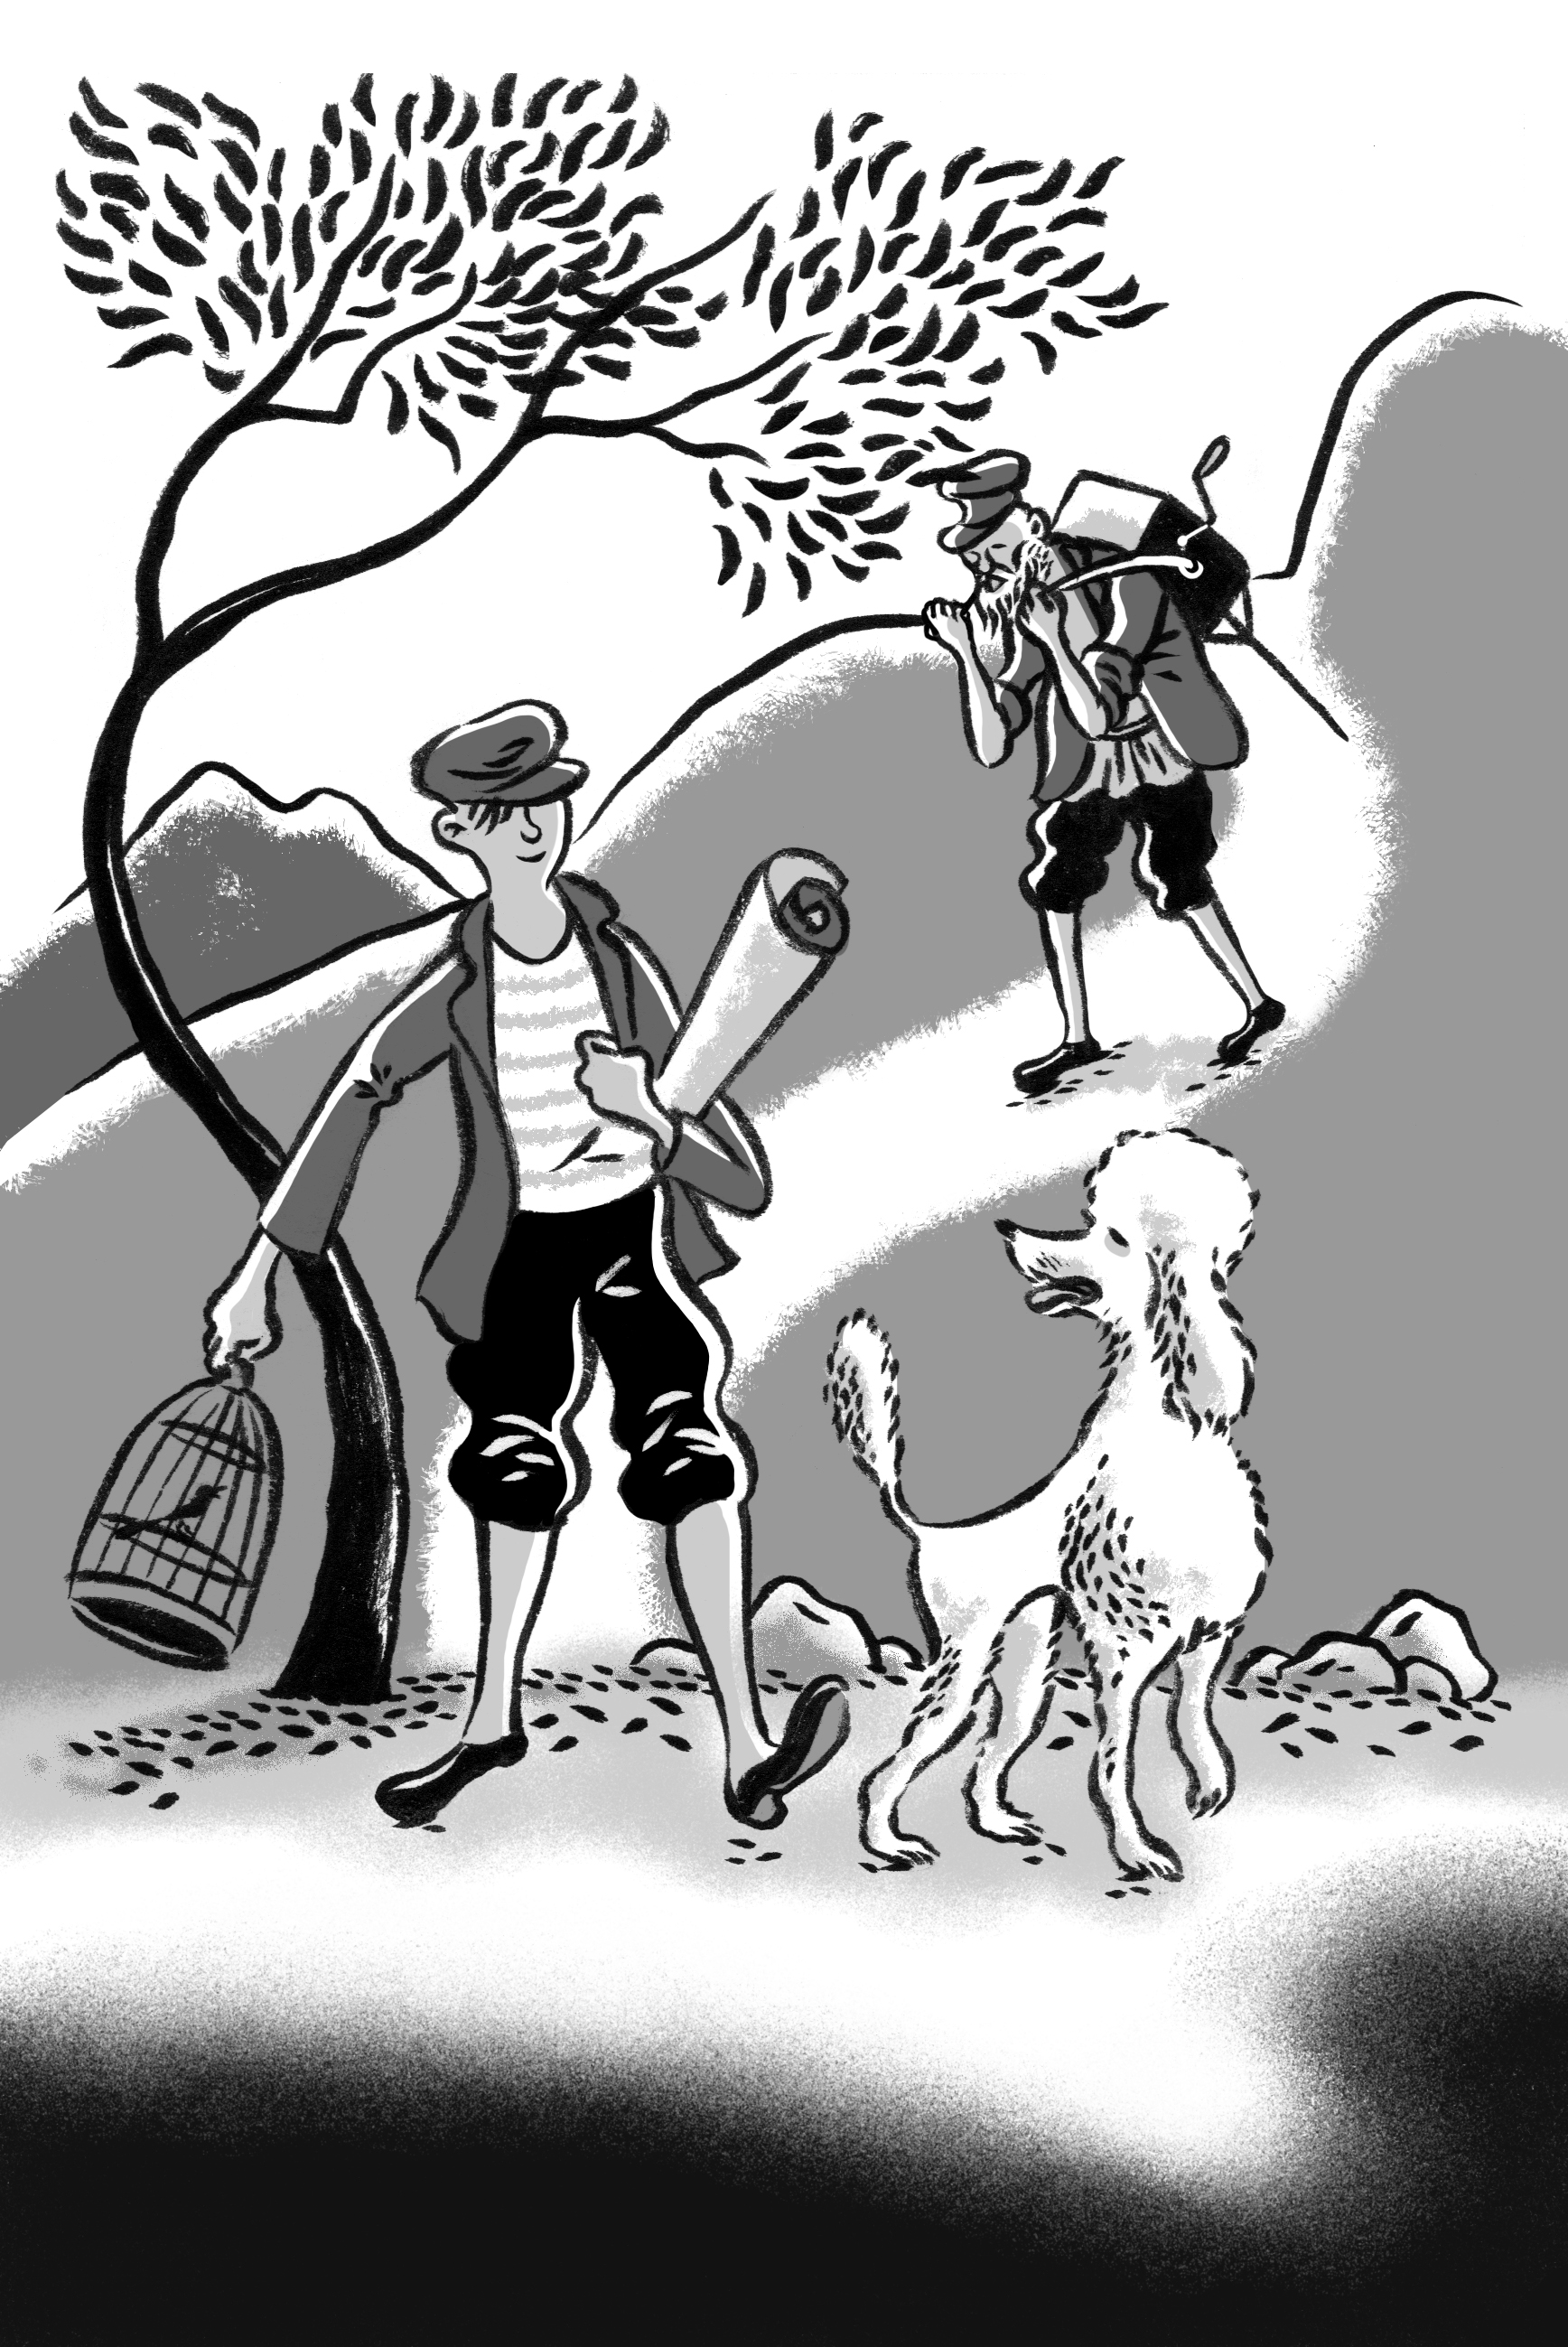
\includegraphics{./imgs/cena10.jpg}
\end{figure}

O velho e o menino deitaram lado a lado sobre a grama, colocando embaixo
das cabeças seus velhos paletós dobrados. Sobre eles farfalhava a
folhagem escura dos carvalhos tortos e frondosos. E através dela surgia
o azul de um céu limpo. O riacho, correndo de pedra em pedra, soava de
maneira tão regular e insinuante, que poderia enfeitiçar alguém com
esses murmúrios hipnóticos. O velho se revirava, dava gemidos e falava
algo, mas a Serguei parecia que sua voz vinha de algum lugar distante,
suave e terno, e as palavras eram incompreensíveis como em um conto de
fadas.

--- Em primeiro lugar, vou comprar um traje de acrobata para você:
cor"-de"-rosa com detalhes em ouro\ldots{} Os sapatos também cor"-de"-rosa, de
cetim\ldots{} Em Kiev ou Khárkov ou, digamos, na cidade de Odessa, ali, meu
caro, tem cada circo! Lamparinas a perder de vista\ldots{} E luzes acesas em
todo lugar\ldots{} Um mundaréu de gente, cinco mil pessoas ou mais\ldots{} Como
vou saber? Inventaremos um sobrenome para você, sem falta um italiano. O
que vale um Estiféiev ou, digamos, um Lodýjkin? Nadica, não há nenhuma
imaginação neles. Mas nos cartazes você será Antonio ou, quem sabe,
Enrico ou Alfonso\ldots{}

O garoto não ouvia mais nada. Uma sonolência doce e terna tomou conta
dele, paralisando seu corpo e tirando"-lhe as forças. Vovô Lodýkin também
adormeceu, perdendo repentinamente o fio de suas divagações preferidas
de depois do almoço sobre o futuro brilhante de Serguei no circo. Em
algum momento, durante seu sono, Martyn teve a impressão de que Artô
rosnou para alguém. Por um instante, uma lembrança semiconsciente e
inquietante sobre aquele caseiro de camisa cor"-de"-rosa passou pela mente
enevoada do velho, mas, vencido pelo sono, pelo cansaço e pelo calor,
ele não conseguiu se levantar e apenas chamou pelo cão, preguiçosamente
e de olhos fechados:

--- Artô\ldots{} para onde vai? Venha cá, sem"-vergonha!

Mas os pensamentos dele logo emaranharam e dissiparam"-se em visões
disformes.

A voz de Serguei o despertou. O menino corria de lá para cá pela beira
do riacho, assoviando e gritando com estridência, aflito e assustado:

--- Artô, \emph{ici}! Volte! Psiu! Psiu! Psiu! Artô, volte!

--- O que houve, Serguei? Por que está gritando? --- perguntou Lodýjkin,
incomodado, desdobrando com dificuldade o braço adormecido.

--- Vacilamos, é isso que houve! --- irritado, o menino respondeu
grosseiramente. --- O cachorro desapareceu.

Ele assoviou de maneira cortante e mais uma vez deu um grito prolongado:

--- Artô"-ô"-ô!

--- Pare de inventar histórias! Ele vai voltar --- respondeu Lodýjkin.
No entanto, rapidamente se levantou e pôs"-se a chamar pelo cachorro com
a voz aguda de velho, brava e rouca de sono.

--- Venha cá, Artô, filho de uma cachorra!

Com passos curtos e desnorteados, ele atravessou às pressas a ponte e
subiu, sem parar de chamar pelo cachorro. À sua vista, estendia"-se quase
meio quilômetro do pavimento branco e regular de uma estrada vazia, sem
nenhuma figura ou sombra.

--- Artô! Artôchenka!\footnote{Artôchenka, diminutivo de Artô.} ---
uivou o velho com angústia.

De repente, ele parou, inclinou"-se e ficou de cócoras.

--- Aí está! --- disse o velho com a voz enfraquecida. --- Serguei!
Serioja, venha cá.

--- Que é? --- indagou o menino, ríspido, aproximando"-se de Lodýjkin.
--- Achou um tesouro?

--- Veja, Serioja, o que é isso? Isso aqui? Você entende? --- perguntava
o velho Martyn em voz quase inaudível.

Ele encarou o menino com olhos perdidos e cheios de dor, enquanto sua
mão, apontada para o solo, balançava de um lado para outro.

Sobre a poeira branca da estrada, um grande pedaço de linguiça, comido
pela metade, estava jogado e, ao redor, por todo lado, se espalhavam
pegadas de cachorro.

--- Levou o cão embora, canalha! --- sussurrou o velho, assustado, ainda
de cócoras. --- Só pode ter sido ele, está claro como o dia\ldots{} Lembra
como na beira do mar ele deu linguiça para Artô?

--- Tão claro como o dia --- repetiu Serguei, sombria e furiosamente.

Os olhos escancarados do velho de repente começaram a piscar,
debulhando"-se em lágrimas. Ele as cobriu com as mãos.

--- O que faremos agora, Serioja? Hem? O que faremos? --- repetiu o
velho, oscilando para a frente e para trás, soluçando, impotente.

--- O que faremos? --- imitou"-o Serguei. --- Levante"-se, vovô Lodýjkin,
Vamos!

--- Vamos\ldots{} --- repetiu o velho, desanimado e obediente, levantando"-se.
--- Pois é, vamos, meu querido\ldots{}

Serguei perdeu a paciência e gritou com vovô Lodýjkin como se este fosse
uma criança:

--- Chega de choramingar, velho. Onde é que se viu uma coisa dessas?
Apanhar o cachorro dos outros? Por que está piscando os olhos para mim?
Não tenho razão? Iremos lá e diremos sem rodeios: ``Devolva nosso
cachorro!''. Senão, iremos ao juiz de paz. E ponto"-final!

--- Ao juiz, ah é\ldots{} Claro\ldots{} Você está certo\ldots{} --- repetia Lodýjkin
com um sorriso amargo e disparatado no rosto, enquanto seus olhos se
agitavam, confusos e constrangidos. --- Ao juiz\ldots{} Sim\ldots{} Só que tem uma
coisa, Serioja\ldots{} Essa coisa de juiz não vai bem\ldots{}

--- Como não vai bem? A lei é para todos. Para que ficar cheio de não me
toques com ele? --- interrompeu o menino, impaciente.

--- Olhe, Serguei, não fique bravo comigo. Eles não vão devolver nosso
cachorro --- vovô Lodýjkin abaixou o tom da voz, misterioso. --- Estou
preocupado com a história do passaporte. Escutou o que aquele doutor
falou? Perguntou se eu tinha um passaporte. Aí é que está, Serguei. É
que eu tenho --- uma expressão de pavor imprimiu"-se no rosto do velho
--- o passaporte de outro homem --- dizia em voz tão baixa, que mal se
ouvia.

--- Como, de outro homem?

--- É assim\ldots{} Perdi o meu na cidade de Taganrog ou, quem sabe, o
roubaram. Uns dois anos eu me virei sem ele: me escondia, dava propinas,
enviava requerimentos\ldots{} Até que percebi que não havia jeito de
continuar assim. Vivia feito um coelho, sempre fugindo. Uma vida sem
sossego. E, de repente, em Odessa, topei com um grego em uma hospedaria.
``É mole'', disse. ``Dê vinte e cinco pratas, velho, que eu lhe forneço
um passaporte para toda a vida.'' Eu pensei com meus botões que estava
perdido de qualquer maneira e concordei. Assim, desde então, meu
querido, eu vivo com o passaporte de outro homem.

\textls[-5]{--- Ah, vovô, vovô! --- o menino deu um suspiro profundo e lacrimoso.
--- É pena perder o cachorro\ldots{} Um cão tão maravilhoso\ldots{}}

--- Ah, Serioja, meu querido! --- o velho esticou os braços trêmulos na
direção do garoto. --- Se eu estivesse com o passaporte verdadeiro, acha
que me importaria com o fato de serem \emph{millionnaires}? Eu os pegaria
pela garganta! ``Como é que é? Com licença! Que direito têm de roubar
cachorros alheios? Sob qual lei o fazem?'' Mas, agora, estamos com as
mãos atadas, Serioja. Se eu for à polícia, a primeira coisa que falarão
é: ``Cadê seu passaporte? Você é Martyn Lodýjkin, pequeno comerciante de
Samara?''. ``Eu, Excelência.'' Só que não sou nem Lodýjkin nem
comerciante, sou o camponês Ivan Dúdkin. E não faço ideia de quem seja
Lodýjkin, que Deus o proteja. De repente é um ladrão ou um condenado
fugitivo? Ou, ainda, um assassino? Não, Serioja, não há nada que se
possa fazer neste caso\ldots{} Nada, Serguei\ldots{}

A voz dele se calou, sufocada. Lágrimas escorriam por suas rugas
profundas e marrons de sol. Serguei, pálido de preocupação e com as
sobrancelhas franzidas, escutava em silêncio o velho enfraquecido
quando, subitamente, o agarrou por baixo dos braços e começou a
levantá"-lo.

--- Vamos, vovô --- disse ele de forma imperativa e ao mesmo tempo
terna. --- Que o passaporte vá para inferno! Vamos lá! Não quer passar a
noite no meio da estrada, quer?

--- Meu querido, meu menino --- disse o velho, tremendo por inteiro ---,
o cachorrinho era excepcional\ldots{} Nosso Artôchenka\ldots{} Nunca encontraremos
outro como ele\ldots{}

\textls[-45]{--- Está bem, já chega\ldots{} Levante"-se --- Serguei dava ordens. ---
Deixe"-me tirar essа sua poeira. Não pode ficar nesse desânimo, vovô.}

Nesse dia os saltimbancos não trabalharam mais. Apesar da pouca idade,
Serguei compreendia muito bem o significado fatal da terrível palavra
``passaporte''. Por essa razão, ele não insistiu em novas buscas por
Artô, nem no juiz de paz, nem em outras medidas categóricas. Mas,
enquanto ele caminhava ao lado do velho até uma hospedaria, de seu rosto
não saía uma expressão inédita, compenetrada e obstinada, era como se
ele arquitetasse um plano grande e muito importante.

Sem terem combinado, mas evidentemente atraídos pelo mesmo desejo, deram
uma volta proposital e significativa, para mais uma vez passar na frente
da ``Vila da Amizade''. Eles se detiveram diante do portão na
expectativa vaga de ver Artô ou ao menos de ouvir seu latido ao longe.

Mas os portões trançados da luxuosa \emph{datcha} estavam bem fechados
e, no jardim sombreado sob ciprestes tristes e esbeltos, fazia um
silêncio imperturbável, sufocante e imponente.

--- Pa"-trões! --- resmungou o velho, depositando nessa palavra toda a
mágoa ardente que transbordava de seu coração.

--- Deixe para lá, vamos --- ordenou severamente o menino, puxando"-o
pela manga.

--- Serioja, pode ser que Artô ainda fuja deles, hem? --- o velho pôs"-se
a soluçar novamente. --- Será? O que acha, meu querido?

Mas o garoto não respondeu. Continuava a caminhar а passos largos e
determinados. Seus olhos obstinados fitavam a estrada e as sobrancelhas
delicadas franziam furiosamente.

\section{6}

Em silêncio chegaram até a cidade de Alupka. O velho gemeu e suspirou o
caminho todo, enquanto Serguei manteve a expressão brava e decidida.
Pararam para pernoitar numa taberna turca e suja chamada Yildiz, que em
turco significa ``estrela''. Eles se acomodaram com pedreiros gregos,
escavadores turcos, alguns operários russos que viviam de trabalhos
temporários e ainda alguns tipos sombrios e suspeitos, daqueles que são
vistos com frequência vagando pelo sul da Rússia. Assim que a taberna
fechou, na hora determinada, todos se deitaram em bancos dispostos ao
longo das paredes ou direto no chão. Os mais experientes, por necessária
precaução, colocaram embaixo de suas cabeças os pertences --- roupas,
objetos --- mais preciosos que tinham.

Já havia passado muito da meia"-noite quando Serguei, deitado no chão ao
lado do vovô, se levantou cautelosamente e começou a se vestir sem fazer
barulho. Pelas janelas largas do quarto, jorrava a luz pálida da lua,
que desenhava no chão uma cerca trêmula e inclinada e iluminava os
rostos das pessoas, deitadas de qualquer jeito, dando"-lhes um aspecto
sofrido e sem vida.

--- Onde garroto ir tão tarde? --- indagou a voz sonolenta do dono da
taberna, o jovem turco Ibrahim, quando o menino se aproximou da porta.

\textls[-15]{--- Deixe"-me sair. É preciso! --- retrucou Serguei com o ar sério de um homem de negócios. --- Vá, levante a carcaça daí, turco!}

Bocejando, coçando"-se e estalando a língua em sinal de desaprovação,
Ibrahim destrancou a porta. As ruas estreitas do mercado tártaro estavam
mergulhadas numa densa sombra azul"-escura, que cobria o pavimento com
reflexos em forma de dentes e tocava as soleiras das casas do lado
iluminado, com suas paredes baixas brilhando sob a luz branca e intensa
da lua.

Ao longe, na extremidade da região, ouviam"-se latidos de cães. De algum
lugar, da estrada de cima, soou um tropel de cavalos em marcha rápida e
cadenciada.

Depois de passar por uma mesquita branca com a cúpula verde em forma de
cebola, cercada pelo conjunto silencioso de ciprestes escuros, o menino
desceu por uma travessa estreita e sinuosa e chegou à estrada de baixo.
Para ficar mais leve, Serguei não vestiu a roupa de cima, usando apenas
o macaquinho de tricô. A lua caía"-lhe nas costas e a sombra dele corria
à frente, formando uma silhueta preta, estranha e encurtada. Pelos dois
lados da estrada, escondiam"-se arbustos escuros de folhagem pujante. Um
passarinho gritava de dentro deles, em intervalos regulares, com uma voz
fina e submissa: ``Que so"-o"-no!\ldots{}''. Parecia vigiar humildemente, na
escuridão da noite, um segredo triste, lutando, impotente, contra o sono
e o cansaço e lamentando baixinho, sem esperança: ``Que so"-o"-no!\ldots{}''. Em
cima dos arbustos e dos cumes azulados de florestas longínquas,
erguia"-se, apoiando"-se no céu com seus dois picos, o monte Ai"-Petri,
leve, nítido e flutuante, como se tivesse sido recortado de um pedaço
gigante de cartolina prateada.

Serguei sentiu arrepios no meio desse silêncio majestoso, em que seus
passos ecoavam de forma nítida e perturbadora, mas, ao mesmo tempo, em
seu coração crescia uma valentia excitante e impetuosa. Em uma das
curvas da estrada, o mar abria"-se de repente. Imenso e calmo, ele
ondulava de maneira pacífica e solene. Do horizonte até a costa, uma
faixa estreita e prateada tremulava. No meio do mar, ela desaparecia,
apenas por vezes cintilando, mas, ao chegar perto da terra, a faixa se
derramava abundantemente como um metal vivo e brilhante, contornando a
margem.

O garoto atravessou silenciosamente uma cancela de madeira que conduzia
ao parque. Ali, entre árvores densas, erguia"-se uma completa escuridão.
Ao longe ele ouvia o ruído incessante do riacho e sentia a respiração
fria e úmida. Sob seus pés o soalho amadeirado da ponte ecoava
ruidosamente. As águas negras por baixo dela o assustavam. Por fim,
surgiram os altos portões trançados de ferro envolvidos pelos caules
rastejantes das glicínias. A luz da lua, perpassando pelas copas das
árvores, deslizava pelos entalhes dos portões em manchas fracas e
fosfóricas. Do outro lado, no escuro, havia uma quietude vigilante,
pronta a ser rompida.

\textls[-15]{Em alguns momentos Serguei hesitou, quase apavorado, mas conseguiu
dominar esses sentimentos angustiantes e sussurrou:}

--- Eu vou mesmo assim! Não importa!

Ele não teve dificuldade para escalar os portões. As espirais de ferro
que compunham o trançado serviram de apoio para suas mãos ágeis e as
pequenas pernas musculosas. Em cima dos portões, numa altura
considerável, havia um grande arco de pedra que ligava um poste ao
outro. Serguei, tateando, subiu no arco, depois, apoiando"-se na barriga,
desceu as pernas no outro lado e começou, aos poucos, a empurrar o
tronco para lá, sempre procurando com os pés uma saliência. Assim, ele
ficou com quase todo o corpo pendurado do outro lado do arco, agarrando
a beirada com os dedos das mãos esticadas, mas seus pés não encontravam
um apoio. Ele não cogitou na hora que, na parte de dentro, o arco
sobressaía mais ao portão, e à medida que suas mãos adormeciam e seu
corpo exaurido ficava mais pesado, o menino era invadido por um medo
apavorante.

Por fim, Serguei não aguentou. Seus dedos, que agarravam um canto
pontiagudo, se abriram e o garoto impetuosamente despencou.

Ele ouviu o cascalho estalar debaixo de seu corpo e sentiu uma dor aguda
nos joelhos. Por alguns instantes permaneceu de gatinhas, aturdido
pela queda. Teve a impressão de que todos os moradores da casa iriam
despertar, que o caseiro sombrio de camisa cor"-de"-rosa viria correndo,
que haveria gritos e confusão\ldots{} Mas o silêncio profundo e imponente
continuava a reinar no jardim. Apenas um zunido baixo e monótono
espalhava"-se ao redor:

``Zzz"-zzz"-zzz\ldots{}''.

``Ah, deve vir de dentro do ouvido!'', supôs Serguei. Ele se levantou:
nesse jardim repleto de sonhos e cheiros, tudo era assustador,
misterioso e lindo como num conto de fadas. As flores, que mal podiam
ser vistas na escuridão, balançavam suavemente nos canteiros,
inclinando"-se uma à outra com uma inquietação vaga, como que cochichando
e bisbilhotando. Com ar pensativo e perscrutador, os esbeltos ciprestes,
escuros e perfumados, acenavam lentamente com os cumes afinados. Atrás
do riacho, nos arbustos densos, o passarinho extenuado lutava contra o
sono e repetia seu humilde lamento:

``Que so"-o"-no!\ldots{} Que so"-o"-no!\ldots{}''.

De madrugada, no meio das sombras entrelaçadas das sendas do jardim,
Serguei não reconhecia o lugar. Por muito tempo vagou pelo cascalho
rangente, até que, enfim, chegou ao casarão.

Nunca em sua vida ele tivera a penosa sensação de completa impotência,
abandono e solidão como agora. A casa parecia repleta de inimigos
dissimulados e impiedosos que, escondidos atrás das janelas escuras,
observavam com sorrisos maliciosos cada movimento do pequeno e frágil
menino. Calados e impacientes, esperavam por um sinal, por um comando
terrível, furioso e ensurdecedor.

--- Dentro de casa não\ldots{} Ele não pode estar lá dentro! --- sussurrou o
menino, delirante. --- Lá começaria a uivar e a importunar\ldots{}

Ele deu a volta. Na parte de trás, num pátio largo, havia outras
construções mais simples, menos rebuscadas, pelo visto destinadas aos
empregados. Ali, como na casa grande, nenhuma janela estava acesa;
apenas a lua se refletia nos vidros escuros com uma luz irregular e
opaca. ``Não há como sair daqui, nunca conseguirei!\ldots{}'', pensou Serguei
com angústia. Ele se lembrou num átimo do vovô, do velho realejo, das
noites nas tabernas, das refeições perto de nascentes refrescantes.
``Não haverá mais nada disso\ldots{} Nunca mais!'', repetiu tristemente
consigo. E, quanto mais desesperados se tornavam seus pensamentos, mais
o medo dentro dele cedia lugar a uma espécie de ansiedade raivosa,
imperturbável e obtusa.

De repente, o garoto ouviu um ganido fino e queixoso. Ele parou e, mal
respirando, com os músculos tensionados, ficou na ponta dos pés. O som
se repetiu. Parecia vir de perto de Serguei, de um porão de pedra que se
comunicava com o exterior por meio de uma fileira de pequenas aberturas
retangulares sem vidro. Pisando nas flores de um canteiro, ele
aproximou"-se da parede, encostando o rosto em um dos orifícios, e
assoviou. Um ruído baixo e cauteloso soou de algum lugar embaixo e no
mesmo instante cessou.

--- Artô! Artô! --- chamou Serguei com um sussurro trêmulo.

Um latido entrecortado e incontido preencheu o jardim, ecoando por todos
os cantos. Nesse ladrar, à saudação feliz se misturaram queixume, raiva
e dor física. O menino podia ouvir o cachorro se debatendo com ímpeto no
porão escuro, tentando livrar"-se de algo.

--- Artô! Meu cãozinho!\ldots{} Artôchenka!\ldots{} --- Serguei dizia entre
lágrimas.

--- Psiu, cachorro maldito! --- ressoou de baixo uma voz grave e
selvagem. --- Quieto, condenado!

Algo bateu no porão. O cão disparou uivos longos e intermitentes.

--- Não se atreva a bater! Não se atreva a bater no cachorro, canalha!
--- gritou o garoto fora de si, raspando com as unhas o muro de pedra.

Tudo o que aconteceu depois baralhou"-se na memória de Serguei, como uma
espécie de delírio febril. A porta do porão se escancarou com estrondo e
dela saiu o caseiro. Com roupas de baixo, barbudo, descalço e
empalidecido pela luz intensa da luz que lhe caía diretamente no rosto,
ele lembrava a Serguei um monstro gigantesco e furioso de conto de
fadas.

--- Quem está aí?! Vou atirar! --- sua voz trovoava pelo jardim. ---
Ladrões! Assalto!

Nesse instante, do vão escuro da porta aberta saiu saltando, como uma
bola branca, Artô, latindo sem parar. Em seu pescoço balançava um resto
de corda.

No entanto, o menino não prestava atenção no cachorro. A aparência
ameaçadora do caseiro lhe deu um medo sobrenatural, os pés do artista
grudaram"-se ao chão e seu corpinho delicado paralisou. Mas, felizmente,
essa aflição não durou muito tempo. Quase inconsciente, Serguei deu um
grito desesperado, longo e agudo e precipitou"-se para fora do porão,
desnorteado, sem ver o caminho, sem domínio de seus atos.

Ele corria em disparada, parecia um pássaro voando, golpeava
seguidamente a terra com os pés, que, de repente, tornaram"-se fortes
como duas molas de aço. Ao seu lado saltitava Artô e seus latidos
felizes inundavam o ar. Atrás deles, o furioso caseiro ressoava na
areia, praguejando.

No impulso, Serguei quase se bateu contra os portões, mas
instantaneamente, sem pensar, teve a intuição de que ali não havia
saída. Entre o muro e os ciprestes que cresciam ao longo dele,
estendia"-se uma passagem estreita e escura. Sem hesitar, sob comando do
medo, o menino penetrou ali e esgueirou"-se, correndo abaixado pela
passagem. As folhas afiadas dos ciprestes, cheirando fortemente a
resina, chicoteavam"-lhe o rosto. Ele tropeçava nas raízes e caía,
machucando as mãos a ponto de sangrar, mas rapidamente se levantava, sem
se importar com a dor, e prosseguia com a corrida, curvado, sem ouvir o
próprio grito. Artô o seguia.

Serguei corria pelo estreito corredor formado, de um lado, pelo muro
alto e, de outro, pela fileira apertada de ciprestes, corria como um
animalzinho enlouquecido depois de ter caído numa armadilha sem saída.
Sua boca ressecou e, a cada respiro, sentia milhares de agulhadas no
peito. As batidas de pés do caseiro vinham ora da direita, ora da
esquerda, e o menino, perdendo a cabeça, atirava"-se ora para a frente,
ora para trás, passando várias vezes do lado dos portões e enfiando"-se
de novo na passagem estreita e escura.

Finalmente as forças o abandonaram. Aos poucos o pavor indômito deu
lugar a uma angústia fria e indolente, a uma indiferença surda a
qualquer ameaça. Ele se sentou embaixo de uma árvore, encostando o corpo
esgotado no tronco e semicerrou os olhos. Os passos pesados do inimigo
ressoavam sobre a areia cada vez mais perto. Artô gania em voz baixa,
colocando o focinho nos joelhos do pequeno acrobata.

A uns dois passos do menino, galhos começaram a se mexer, separados por
mãos. Ele involuntariamente levantou os olhos e, de repente, tomado por
uma alegria inacreditável, deu um salto no lugar. Só então notou que o
muro diante de si era mais baixo, não passando de um metro. Seu topo, é
verdade, estava forrado por cacos de garrafa fixos em gesso, mas Serguei
nem pensou nisso. Num átimo agarrou Artô pelo meio do corpo e o
colocou com as patas da frente viradas para o muro. O cão esperto o
entendeu de imediato. Rapidamente subiu no muro, abanou o rabo e latiu,
anunciando vitória. Sem demora, o menino se juntou a ele, bem no momento
em que, dos galhos de ciprestes, surgiu uma figura grande e escura. Os
dois corpos ágeis e flexíveis --- do cão e do pequeno acrobata --- fácil
e suavemente saltaram à estrada. Atrás deles caiu uma chuva de
impropérios furiosos.

Fosse o caseiro menos habilidoso do que os dois amigos ou estivesse
cansado das voltas pelo jardim ou, quem sabe, simplesmente nunca tivesse
desejado alcançar os fugitivos, o fato é que parou de persegui"-los. Em
todo caso, eles ainda correram longamente, sem descanso; fortes e
jeitosos, com asas nos pés, felizes com a libertação. A habitual
despreocupação logo voltou ao \emph{poodle}. Serguei ainda olhava
receoso para trás, enquanto Artô dava pulinhos em torno dele, balançando
com entusiasmo as orelhas e o pedaço da corda, que tentava de todo jeito
alcançar com a língua.

O menino só voltou a si quando chegou à nascente, aquela perto da qual,
na véspera, ele comera com o velho. As duas bocas, do cão e do jovem,
sedentas, encostaram ao mesmo tempo na poça gelada, sorvendo
demoradamente a água fresca e deliciosa. Empurravam"-se, tiravam, para
recobrar o fôlego, as cabeças da água, que caía sonoramente de seus
lábios, para em seguida, com a sede renovada, de novo se atirarem à
poça, sem forças para abandoná"-la. Quando, finalmente, deixaram a
nascente e voltaram a caminhar, a água gorgolejava em seus ventres
cheios. O perigo se fora, os horrores dessa noite passaram sem deixar
rastros, e ambos caminhavam aliviados e felizes pela estrada branca,
iluminada pela lua e cercada por arbustos escuros que já exalavam a
umidade da manhã e o aroma adocicado das folhas frescas.

Na taberna Yildiz, Ibrahim encontrou o garoto com ar de reprovação e
sussurrou:

--- Por que o garroto está sempre vagamundeando? Para que vagamundear?
Ai"-ai"-ai, nada bom\ldots{}

Serguei não queria acordar o velho saltimbanco, mas Artô fez isso no seu
lugar. Num instante o encontrou entre os vários corpos largados no chão
e, antes de ele recobrar os sentidos, o cachorro já lhe lambia, com
ganidos felizes, as faces, os olhos, o nariz e a boca. O vovô despertou,
viu a corda no pescoço do \emph{poodle}, viu o menino deitado ao lado,
coberto de poeira, e compreendeu tudo. Ele se dirigiu a Serguei atrás de
explicações, mas nada conseguiu. O menino já dormia profundamente com os
braços jogados para os lados e a boca aberta.


\medskip

{\footnotesize\hfill\emph{Tradução Tatiana Larkina.}}

\chapter{O elefante}\label{part11}

\section{1}

\noindent{}Uma menininha estava doente. Todo dia recebia a visita do doutor
Mikhail Petróvitch, que ela conhecia fazia muito tempo. Às vezes, ele
vinha acompanhado por dois médicos estranhos. Eles viravam a menina de
costas e de bruços, auscultavam aqui e ali, encostando o ouvido em seu
corpo, puxavam sua pálpebra inferior para baixo e observavam. Daí eles
bufavam com importância, de rostos severos, e conversavam entre si numa
língua incompreensível.

Depois, eles passavam do quarto para a sala de estar, onde a mãe os
esperava. O doutor principal --- alto, de cabelos grisalhos e óculos
dourados --- lhe falava longamente, com ar sério. Com a porta aberta, a
menina podia ver e ouvir tudo de sua cama. Ela não compreendia muita
coisa, mas sabia que estavam falando dela. A mãe escutava o médico,
fitando"-o com os olhos grandes e cansados de tanto chorar. Uma vez, ao
se despedir, o doutor principal disse em bom som:

--- O importante é não deixá"-la entediada. Realizem qualquer vontade.

--- Ah, doutor, é que ela não quer nada!

--- Então, não sei\ldots{} Tentem se lembrar do que ela gostava antes de
adoecer. Brinquedos\ldots{} Doces\ldots{}

--- Mas, doutor, ela não quer\ldots{}

--- Bem, deem um jeito de animá"-la\ldots{} Com qualquer coisa\ldots{} Dou minha
palavra: se conseguirem fazê"-la sorrir, alegrá"-la, será o melhor
remédio. Compreenda, a doença de sua filha é o desânimo com a vida, e
nada mais\ldots{} Passe bem, senhora!

\section{2}

--- Nádia,\footnote{Nádia é apelido de Nadiejda, que em russo
  significa ``esperança''.} minha queridinha --- disse a mãe ---, não há
nada que você queira?

--- Não, mamãe, eu não quero nada.

--- Quer que eu coloque suas bonecas aqui, em cima da cama? A gente
podia pôr as poltroninhas, o sofá e a mesinha com o jogo de chá. As
bonecas irão tomar chá e papear sobre o tempo e a saúde dos filhos\ldots{}

--- Obrigada, mamãe\ldots{} Não estou com vontade\ldots{} Estou aborrecida\ldots{}

--- Está bem, querida, deixe as bonecas para lá\ldots{} E se a gente chamasse
suas amigas, a Kátia ou a Jenia? Você gostava tanto delas.

--- Não precisa mamãe. De verdade\ldots{} Não quero nada. Estou tão
aborrecida!

--- Quer que eu traga um chocolate?

Mas a menina não respondeu, fixando os olhos tristes no teto. Ela não
sentia nenhuma dor, nem sequer tinha febre. A cada dia, porém, emagrecia
e enfraquecia. Não importava o quanto se esforçassem, para ela era tudo
igual, continuava sem nada desejar. Assim, dia após dia, ela ficava
deitada, quieta e tristonha. Às vezes, ela cochilava por meia hora, mas
só sonhava com algo cinzento, longo e monótono, como a chuva outonal.

Quando a porta de seu quarto se abria para a sala e a da sala para o
gabinete, a menina conseguia ver seu pai. Ele andava depressa, de um
lado para outro, fumando sem parar. De vez em quando, ele ia ao quarto
de Nádia, sentava"-se na beirada da cama e acariciava distraidamente os
pés da filha. Mas logo se levantava de salto e se aproximava da janela.
Ele assoviava uma melodia qualquer espiando a rua, mas seus ombros
tremiam. Então, apressava"-se em encostar um lenço no canto dos olhos e,
como se estivesse com raiva, disparava de volta para o gabinete. Lá,
voltava a sua marcha acelerada, de um lado para outro, fumando e
fumando\ldots{} Era tanta a fumaça do tabaco, que o ar do gabinete ficava todo
azul.

\section{3}

Um dia, porém, a garotinha acordou um pouco mais animada do que o
habitual. Ela tinha sonhando com algo, mas não conseguia lembrar direito
o que era, e fitou atenta e demoradamente os olhos na mãe.

--- Precisa de algo, meu bem? --- perguntou sua mãe.

Mas a menina, de repente, lembrou o sonho e sussurrou como se
confessasse um segredo:

--- Mamãe\ldots{} Será que eu poderia ter\ldots{} um elefante? Só que não aquele
desenhado no livro\ldots{} Posso?

--- É claro, queridinha, claro que pode!

Sua mãe correu ao gabinete e contou ao pai da menina que esta queria um
elefante. No mesmo instante, ele vestiu o casaco e o chapéu e saiu.

Passada meia hora, estava de volta com um lindo e caro brinquedo. Era um
grande elefante cinza que sabia balançar a cabeça e abanar o rabo. Nas
costas, havia uma sela vermelha e na sela uma pequena marquise dourada
com três homenzinhos sentados embaixo. A menina, no entanto, olhou para
o brinquedo como se olhasse para a parede e o teto, com o mesmo
desânimo, e disse languidamente:

--- Mas não é isso\ldots{} Eu queria um elefante de verdade, um elefante
vivo, e este está morto.

--- Mas, olhe, Nádia --- apressou"-se o pai. --- A gente agora dará corda
nele e ele ficará igualzinho a um elefante de verdade.

Deram corda no elefante e ele, balançando a cabeça e abanando o rabo,
começou a bater os pés, movendo"-se devagar pela mesa. À Nádia nada
disso interessava e ela ficou até mais entediada, mas, para não magoar
o pai, disse em voz baixa, docemente:

--- Muito obrigada, querido papai. Duvido que alguém tenha um brinquedo
tão interessante como esse\ldots{} É que\ldots{} lembra\ldots{} você tinha prometido me
levar ao circo para ver um elefante de verdade\ldots{} E não levou nenhuma
vez\ldots{}

--- Mas, compreenda, minha querida, isso é algo impossível! O elefante
é muito grande, vai até o teto, não caberia na nossa sala\ldots{} E, depois,
onde é que eu vou arranjar um elefante?!

--- Eu não preciso de um muito grande, papai\ldots{} Você pode me trazer um
pequenino, mas um de verdade. Deste tamanho, assim\ldots{} Pode ser um
filhotinho\ldots{}

--- Querida filhinha, eu ficaria feliz em fazer qualquer coisa por
você, mas isso eu não posso. Pois é como se você de repente dissesse:
``Papai, pegue o Sol lá do céu para mim!''.

A menina sorriu, triste.

--- Como você é bobo, papai. Até parece que eu não sei que não se pode
tocar no Sol, pois ele queima. É que nem a Lua. Não, eu só queria um
elefantinho\ldots{} um de verdade.

Ela fechou os olhos devagar e disse baixinho:

--- Estou cansada\ldots{} Desculpe, papai\ldots{}

O pai se agarrou pelos cabelos e disparou para o gabinete. Por algum
tempo, ficou andando de um lado para outro. Em seguida, com um gesto
decidido, apagou a bituca no chão (coisa que sempre o fazia levar uma
bronca da esposa) e gritou para a empregada:

--- Olga! Meu casaco e chapéu!

Sua esposa apareceu na antessala.

--- Aonde você vai, Sacha?\footnote{Sacha, apelido de Aleksándr (e
  Aleksandra).} --- perguntou ela.

Todo ofegante, ele abotoava o casaco:

--- Macha, querida, nem eu sei para onde vou\ldots{} Mas, parece, hoje à
noite eu realmente trarei para cá, para nossa casa, um elefante de
verdade.

A mulher olhou para ele com preocupação.

--- Querido, você se sente bem? Por acaso está com dor de cabeça? Talvez
você não tenha dormido bem essa noite?

--- Eu não preguei o olho! --- respondeu ele, irritado. --- Pelo visto,
você quer saber se eu perdi o juízo? Ainda não. Até logo! De noite
veremos.

Ele desapareceu, batendo com força a porta de entrada.

\section{4}

Duas horas depois lá estava ele no circo, sentado na primeira fileira,
vendo animais adestrados fazerem todo tipo de truques sob comando do
domador. Cães sabidos pulavam, davam cambalhotas e dançavam no ritmo da
música, então compunham palavras com grandes letras de papelão. Os
macacos --- alguns de saias vermelhas e outros de calçolas azuis ---
andavam pela corda e cavalgavam em um \emph{poodle} gigante. Leões
ruivos enormes pulavam por entre arcos flamejantes enquanto uma foca
desajeitada disparava uma pistola. No fim, vieram os elefantes. Eram
três: um grande e dois completamente pequeninos, anões, mas, mesmo
assim, bem maiores do que um cavalo. Era estranho ver aqueles animais
imensos, aparentemente estabanados e truculentos, executarem truques
tão elaborados, que seriam difíceis mesmo para um homem muito
habilidoso. O que mais chamava atenção era o elefante grande. No
começo, ele se erguia sobre as patas traseiras, sentava, plantava
bananeira, andava por garrafas de madeira e rolava em cima de um
barril. Em seguida, virava com a tromba as páginas de um grande livro de
papelão e, finalmente, sentado a uma mesa e paramentado com um babador,
almoçava como um menino de bons modos.

A apresentação terminou. O público se dispersava. O pai de Nádia
aproximou"-se do dono do circo, um alemão rechonchudo. Ele estava apoiado
num tabique de tábuas com um grande charuto preto metido na boca.

--- Perdão --- começou o pai de Nádia. --- Será que o senhor deixaria
seu elefante passar algum tempo na minha casa?

O alemão, de tamanha surpresa, arregalou os olhos e, boquiaberto, deixou
o charuto cair no chão. Lamuriando, ele se curvou, levantou o charuto,
pondo"-o de volta na boca, e só então se pronunciou:

--- O elefante?\ldots{} Na sua casa?\ldots{} Eu não estou entendendo!

Pela expressão dos olhos, via"-se que o alemão também queria perguntar ao
pai de Nádia se este estava com a cabeça no lugar\ldots{} Mas o pai se
apressou a explicar do que se tratava: sua única filha, Nádia, sofria de
uma estranha doença que mesmo os médicos tinham dificuldade de
compreender. Havia mais de um mês que ela não saía da cama, emagrecendo
e enfraquecendo a cada dia, não se interessava por nada, ficava
entediada e, assim, pouco a pouco, se apagava. Os doutores mandaram
entreter a menina, mas ela nada queria; mandaram realizar todas as suas
vontades, mas ela não tinha nenhuma. E, nesse dia, ela havia expressado
o desejo de ver um elefante de verdade. Não haveria algum jeito de
providenciar isso?

E ele acrescentou com a voz trêmula, segurando o alemão pelo botão do
casaco:

--- Então\ldots{} É claro que eu espero que minha filha se recupere\ldots{}
Mas\ldots{} e se\ldots{} Deus me livre\ldots{} de repente a doença terminar mal?\ldots{} Se
a menina der de morrer?\ldots{} Imagine como passarei o resto da vida
atormentado com a ideia de não ter cumprido seu último desejo?!

O alemão franziu o cenho, cismado, coçando a sobrancelha esquerda com o
mindinho. Finalmente, ele perguntou:

--- Bem\ldots{} E quantos anos tem sua filha?

--- Seis.

--- Hum\ldots{} Minha Lisa também tem seis\ldots{} Bem\ldots{} Pois saiba que isso vai
lhe custar caro. Teremos que levar o elefante à noite e, só na noite
seguinte, poderemos trazê"-lo de volta. De dia não dá. Juntaria muito
\emph{publikum,}\footnote{\emph{Publikum,} do alemão, ``público''.}
seria um escândalo. Dessa maneira, eu perderei um dia inteiro de
trabalho, e o senhor deve cobrir o prejuízo.

--- Claro, claro\ldots{} Não se preocupe com isso!

--- Depois: a polícia deixaria um elefante entrar em um prédio?

--- Eu arranjarei tudo, irão permitir.

--- Mais uma pergunta: o dono do prédio deixaria entrar um elefante?

--- Deixaria. Eu mesmo sou o dono do prédio.

--- A"-há! Tanto melhor. E ainda outra pergunta: em que andar o senhor
mora?

--- No segundo.

--- Hum\ldots{} Isso já não é tão bom\ldots{} O senhor teria, em seu prédio, uma
escada larga, um teto alto, uma sala espaçosa, portas amplas e um piso
bem firme? Porque meu Tommy tem 2,3 metros de altura e 2,8 de
comprimento. Além disso, ele pesa 1,8 toneladas.\footnote{Trata"-se
  do elefante asiático (ameaçado de extinção), entre 2 e 3 metros de
  altura, que é menor do que o africano e tem apenas um ``dedo'' na
  ponta da tromba.}

O pai de Nádia refletiu por um instante.

--- Quer saber? --- disse ele em seguida. --- Vamos agora para minha
casa e examinaremos tudo no local. Se precisar, eu mando alargarem a
entrada.

--- Pois muito bem! --- concordou o dono do circo.

\section{5}

Ao cair da noite, o elefante foi levado para a casa da garotinha doente.

Coberto por uma manta branca, ele andava no meio da rua, todo pimpão,
meneando a cabeça, enrolando e desenrolando sua tromba. Apesar da hora
avançada, uma multidão se aglomerou ao redor dele. O elefante, porém,
não se dava por achado --- todo dia ele via centenas de pessoas no
circo. Apenas uma vez ele ficara um pouco aborrecido. Um moleque da rua
atirara"-se embaixo de suas pernas e começara a fazer caras e bocas para
o divertimento dos curiosos. O elefante, então, calmamente lhe tirara
com a tromba o boné e o jogara atrás da cerca vizinha, fincada de
pregos.

O policial encarregado circulava pela multidão tentando dissuadi"-la:

--- Senhores, queiram dispersar! O que é que vocês acharam de tão
extraordinário aqui? Até me surpreende! Como se nunca tivessem visto um
elefante andando na rua\ldots{}

Finalmente, a escolta chegou até o prédio. Na escada frontal, bem como
por todo o caminho do elefante, até a sala de jantar, as portas estavam
abertas de par em par --- fora preciso arrancar com o martelo as
dobradiças dos batentes. Isso já havia acontecido uma vez, quando
trouxeram um enorme ícone milagroso.

Diante da escada, porém, o elefante se deteve, nervoso, e empacou.

--- É preciso dar alguma guloseima\ldots{} --- disse o alemão. --- \emph{Um}
torta ou algo assim\ldots{} Não, Tommy! Shh\ldots{} Calma, Tommy!

O pai de Nádia correu até a padaria mais próxima e comprou um grande
bolo redondo de pistaches. O elefante queria engolir o bolo inteiro, com
embalagem e tudo, mas seu dono lhe deu apenas um quarto. O tira"-gosto,
pelo visto, era do agrado de Tommy, pois ele logo sacou a tromba para
apanhar mais um bocado. O alemão, no entanto, tinha um truque na manga.
Segurando o bolo na mão, ele começou a subir a escada, degrau por
degrau. O elefante, com a tromba esticada e as orelhas abertas, ia atrás
dele. No segundo pavimento, Tommy recebeu mais um pedaço.

Dessa maneira, ele foi levado até a sala de jantar, cujos móveis foram
retirados com antecedência, assim como o chão fora abundantemente
coberto de palha. Prenderam a perna do elefante numa argola de ferro
atarraxada no chão e, em sua frente, colocaram alguns repolhos, cenouras
e nabos frescos. O alemão acomodou"-se ao lado, num sofá. Apagaram as
luzes e foram todos descansar.

\section{6}

No dia seguinte, a menina acordou de manhãzinha e sem demora perguntou:

--- E o elefante?! Ele chegou?

--- Chegou, sim --- respondeu sua mãe. --- Só que ele mandou que antes a
Nádia tomasse um banhozinho, comesse um ovo e bebesse um copo de leite
bem quente.

--- E ele é bonzinho?

--- Muito bonzinho. Coma, meu bem, nós iremos vê"-lo já, já.

--- E ele é engraçado?

--- Um pouco. Vista seu casaquinho.

O ovo foi rapidamente comido e o leite bebido. Colocaram Nádia no
carrinho que ela usava quando era bem pequena e mal andava e a levaram à
sala de jantar.

O elefante revelou"-se bem maior do que a menina tinha imaginado quando o
vira pelos desenhos. Ele quase batia na porta e, no comprimento,
ocupava metade da sala. Sua pele era grossa, com pregas profundas. As
pernas corpulentas pareciam postes. O rabo comprido, na ponta, se
assemelhava a uma vassoura. A cabeça estava coberta de calombos
grandes. As orelhas imensas, feito folhas de bardanas, pendiam para
baixo. Os olhos eram bem pequerruchos, porém inteligentes e bondosos. As
presas haviam sido cortadas. A tromba lembrava uma cobra comprida e
terminava em duas narinas, entre as quais havia como que um dedo móvel e
flexível. Se o elefante esticasse sua tromba em toda a extensão, ele na
certa alcançaria a janela.

\begin{figure}%[ht!]
\vspace*{-2cm}
\hspace*{-2.3cm}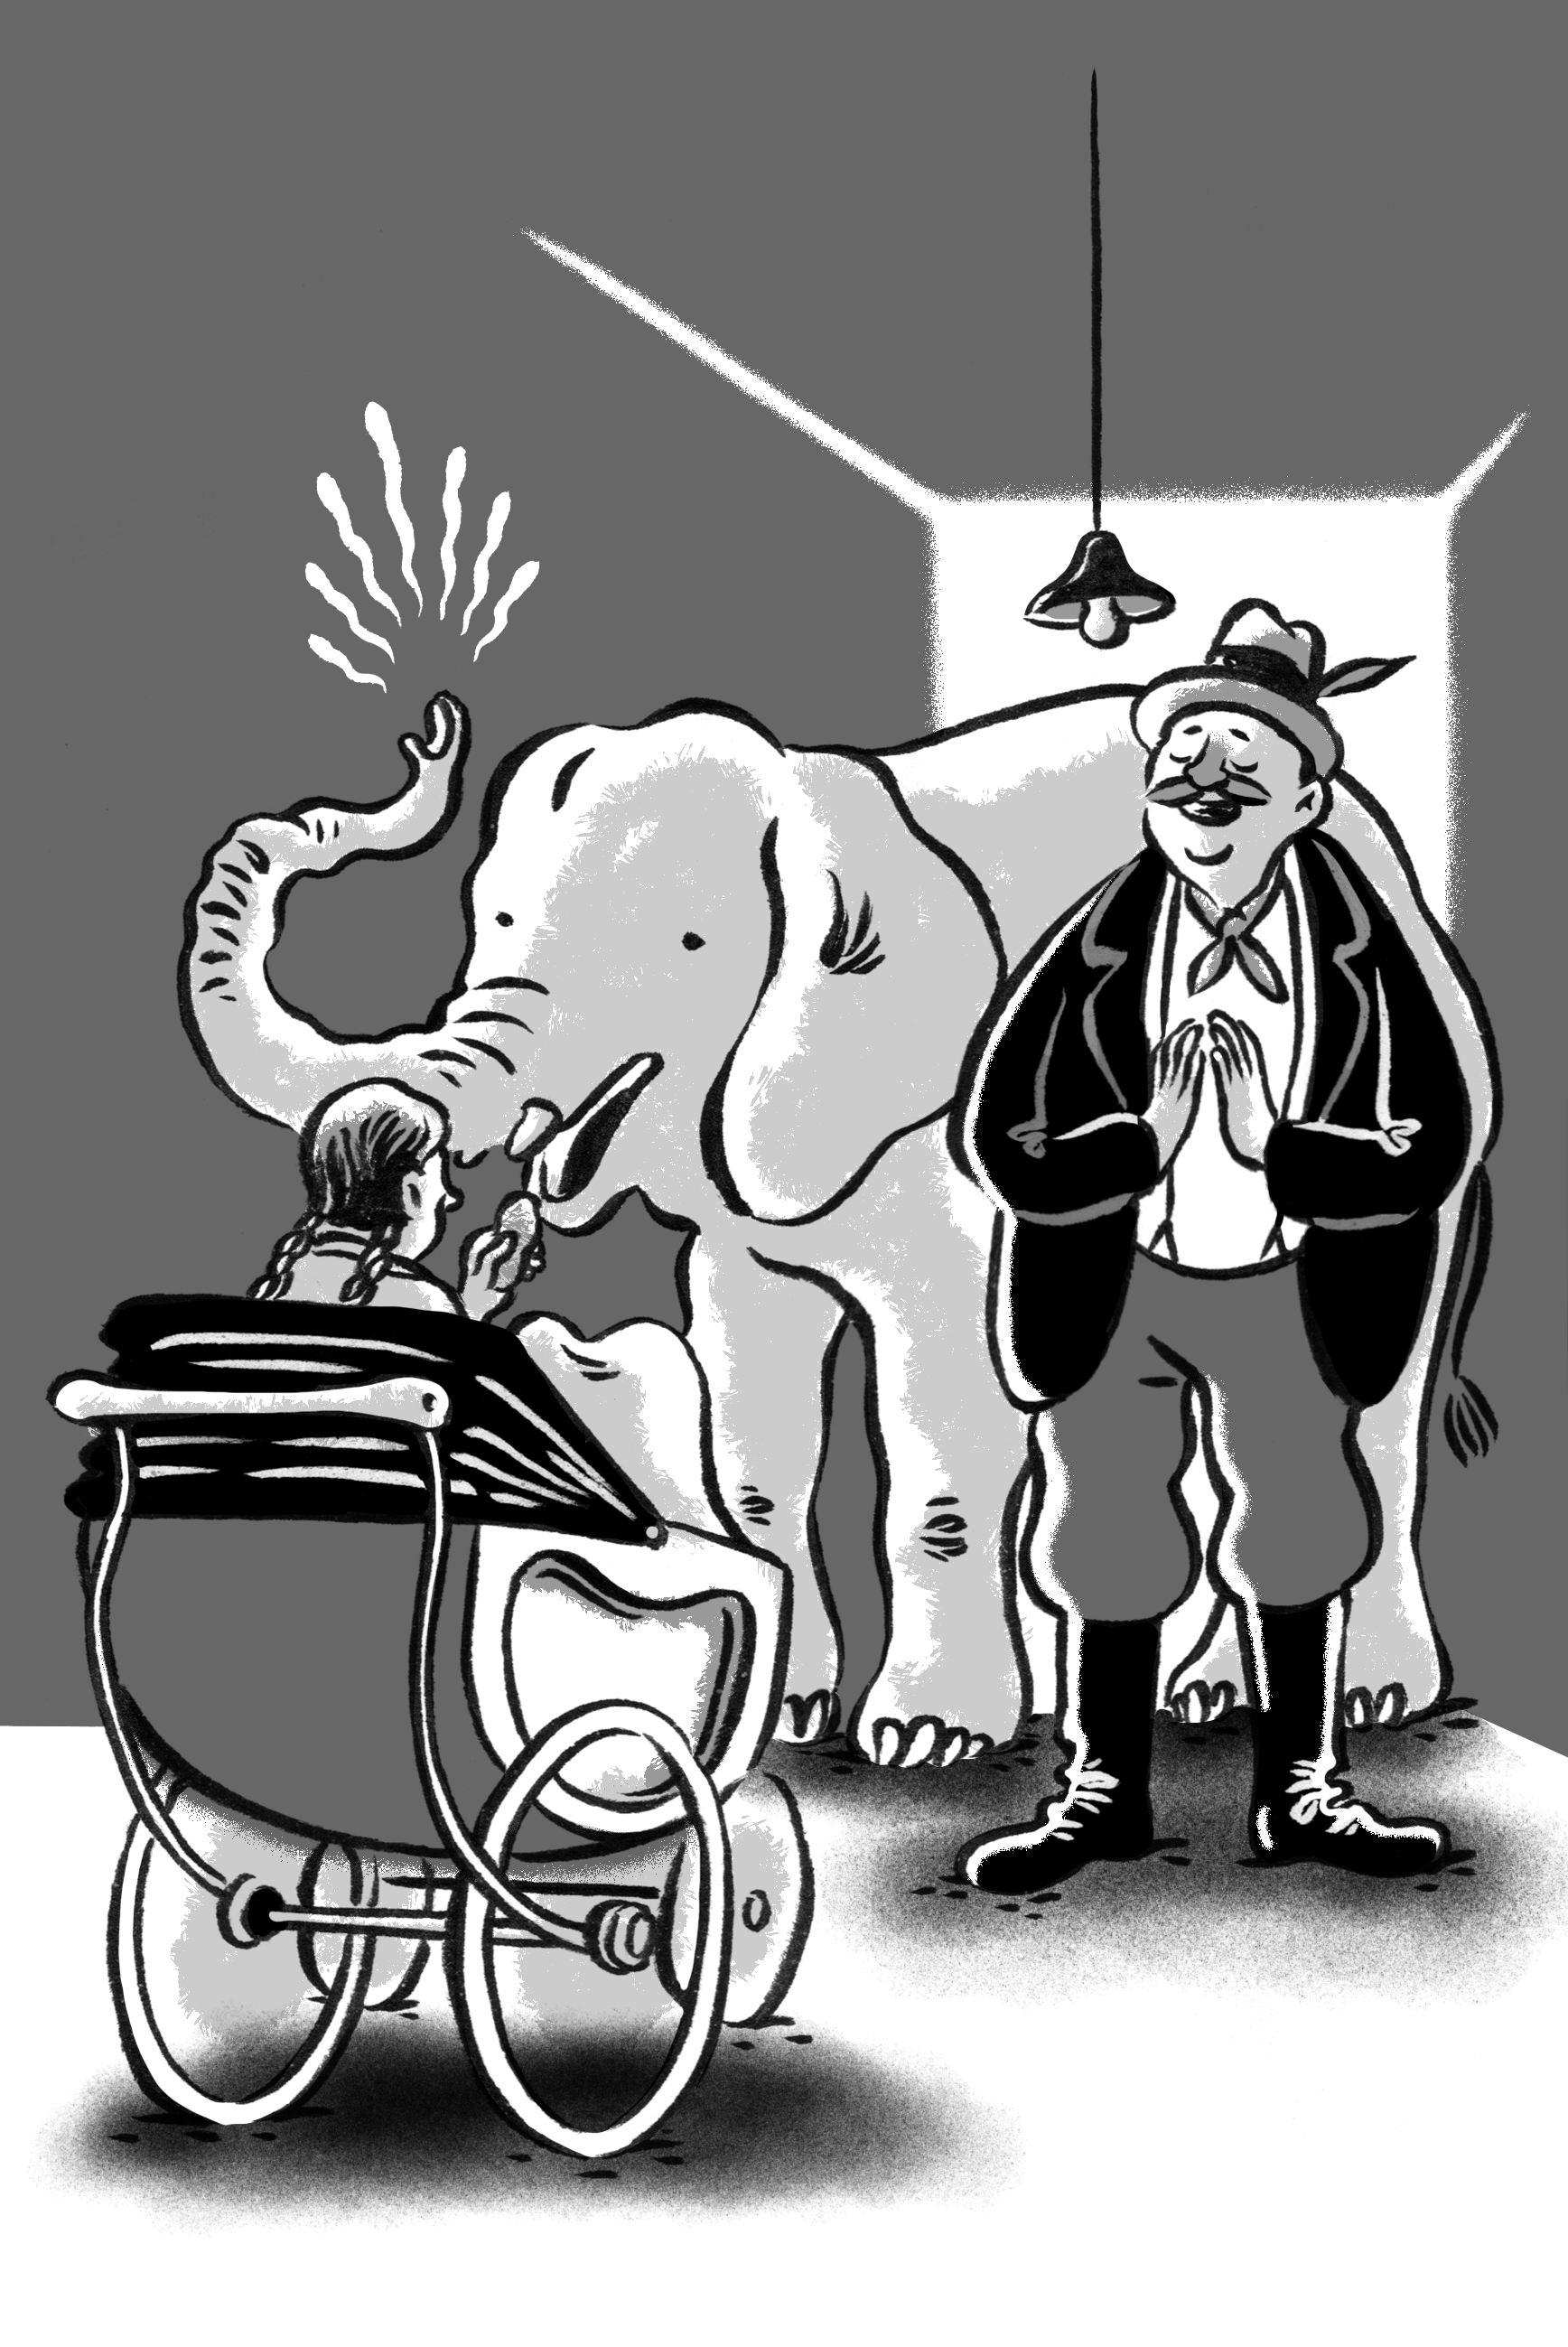
\includegraphics{./imgs/cena11.jpg}
\end{figure}

Entretanto, a menina não parecia assustada. Apenas um pouco chocada com
as dimensões gigantescas do animal. Em compensação, sua babá, Poliana,
uma moçoila de dezesseis anos, começou a gritar de medo.

O dono do elefante aproximou"-se do carrinho e disse:

--- Bom dia, senhorita. Por favor, não tenha medo! O elefante é muito
bonzinho e gosta de crianças.

A menina esticou ao alemão sua pequena mão pálida.

--- Bom dia, como vai o senhor? --- cumprimentou"-o. --- Eu não estou com
medo. Nem um pinguinho. E como ele se chama?

--- Ele se chama Tommy.

--- Bom dia, senhor Tommy --- disse a menina, saudando"-o com a cabeça;
por causa do impressionante tamanho do bicho, ela não se atrevia a
tratá"-lo por \emph{você}. --- O senhor dormiu bem essa noite?

Ela também esticou a mão para ele. O elefante cuidadosamente pegou a
mãozinha dela, apertando seus dedos delicados com o dedo forte e móvel
de sua tromba, e o fez com mais suavidade que o doutor Mikhail
Petróvitch. Com isso, o elefante meneou a cabeça e seus olhos pequenos
tornaram"-se ainda menores, como se sorrissem.

--- Ele entende tudo como parece? --- a menina perguntou ao alemão.

--- Ah, sim, absolutamente tudo, senhorita!

--- Apenas não fala, não é?

--- Pois é. Apenas não fala. Sabe, eu também tenho uma filha, tão
pequena como a senhorita. Ela se chama Lisa. E o Tommy é seu grande
amigo.

--- Sr. Tommy, o senhor já tomou seu chá? --- perguntou ela ao
elefante.

O elefante esticou a tromba outra vez e soprou uma rajada quente bem no
rosto da menina, fazendo seus cabelos leves esvoaçarem para todos os
lados.

Nádia ria e batia as palminhas. O alemão também ria fartamente. Ele era
tão grande, rechonchudo e bonzinho como seu elefante, e a menina tinha a
impressão de que se pareciam. Quem sabe fossem parentes?

--- Não, senhorita, ele não tomou chá. Mas ele aceitaria com prazer água
açucarada. Também adora pãezinhos doces.

Trouxeram uma bandeja com pãezinhos doces e a garota deu de servir ao
elefante. Ele habilidosamente agarrou um pãozinho com o dedo da tromba
e, ao enrolá"-la, fez com que o pão desaparecesse em algum lugar sob a
cabeça, onde se movia seu engraçado e felpudo lá­bio inferior em forma
de triângulo. Dava para ouvir a casca do pão farfalhar em sua pele seca.
Tommy deu o mesmo fim ao segundo pãozinho, assim como ao terceiro,
quarto, quinto. Em sinal de agradecimento, o elefante assentia com a
cabeça, e seus pequenos olhos, de prazer, ficaram ainda mais estreitos.
Feliz, a menina desmachou"-se em risos.

Quando todos os pãezinhos foram comidos, Nádia apresentou suas bonecas
ao elefante:

--- Veja, Sr. Tommy, esta é a Sônia, uma boneca muito elegante. É uma
criança boazinha, mas às vezes fica manhosa e se recusa a tomar a sopa.
Esta é a Natacha, a filha da Sônia. Ela já começou os estudos e conhece
quase todas as letras. E esta daqui é a Matriochka. Foi minha primeira
boneca. O senhor pode ver que ela não tem nariz nem cabelos e a cabeça
foi colada. Mas não se pode expulsar a velhinha de casa, não é, Sr.
Tommy? Antes, ela era a mãe da Sônia, mas agora trabalha como
cozinheira. Então, vamos brincar. O senhor será o pai e eu a mãe; e
elas, nossas filhinhas.

Tommy estava de acordo. Ele deu risada e, em seguida, agarrou Matriochka
pelo pescoço, levando"-a até a boca. Isso, porém, não passava de
brincadeira. Ao mastigar a boneca de leve, ele a colocou inteira no colo
de Nádia --- é verdade que Matriochka voltou um pouquinho amassada e
molhada.

Depois, a menina mostrou ao elefante um grande livro com figuras,
explicando:

--- Aqui está um cavalo, este é um canário, e isto aqui é uma
espingarda\ldots{} Agora uma gaiola com um passarinho, um balde, um espelho,
uma fornalha, uma pá, uma gralha\ldots{} E este aqui, olhe, é um elefante!
Nem parece, não é verdade, Sr. Tommy? Onde já se viu um elefante tão
pequeno?

Tommy ponderou que elefantes tão minúsculos nunca poderiam existir no
mundo. A figura, pelo visto, não lhe agradou. Ele pegou com o dedo na
pontinha da página e a virou.

Chegou a hora do almoço, mas não havia jeito de separar a menina de seu
amigo. O alemão veio socorrer:

--- Permitam"-me resolver isso. Eles vão almoçar juntos.

Ele mandou o elefante sentar. Tommy, obediente, sentou"-se, o que fez o
chão do apartamento estremecer, a louça tilintar no bufê, e reboco cair
do teto dos inquilinos de baixo. A menina foi acomodada em frente.
Colocaram uma mesa entre os dois. Uma toalha de mesa foi atada ao
pescoço de Tommy e os novos amigos começaram sua refeição. Nádia comeu
canja e uma almôndega e o elefante diversos legumes e alface. Em
seguida, deram à menina um minúsculo cálice de xerez e a Tommy uma
tigela de água morna misturada a um copo de rum, e ele se deliciou com a
bebida, sugando"-a pela tromba. Por fim, ganharam a sobremesa: para a
garota, uma xícara de chocolate quente; para o elefante, metade de um
bolo --- dessa vez, um de nozes. Enquanto isso, o alemão estava na sala
de estar em companhia do pai de Nádia e, com o mesmo prazer do elefante,
bebia cerveja, porém em quantidades maiores.

Após o almoço, o pai recebera visitas, que, para não se assustarem,
foram avisadas, logo na antessala, sobre o elefante. No início, elas não
acreditaram, mas, ao ver Tommy, se espremeram na porta de entrada.

--- Não tenham medo, ele é bonzinho! --- Nádia tentou acalmá"-los.

Os visitantes irromperam na sala de estar e, após cinco minutos, deram
no pé.

Anoiteceu. A menina precisava dormir. Mas era impossível tirá"-la de
perto do elefante. Assim, ela acabou adormecendo ao lado dele e, já
sonolenta, foi levada para seu quartinho. Ela nem notou que a trocaram.

Nessa noite, Nádia sonhou que havia se casado com Tommy e que tiveram
uma penca de filhos, alegres elefantinhos. O elefante, que durante a
noite fora levado de volta para o circo, também sonhou com a meiga e
carinhosa garotinha. E também com muitos bolos de nozes e de pistaches,
bolos gigantescos, do tamanho de um portão\ldots{}

Na manhã seguinte, a menina acordou revigorada e bem"-disposta, e, como
nos velhos tempos, quando gozava de plena saúde, gritou alto e
impacientemente para que todos em casa a ouvissem:

--- Lei"-ti"-nho!

Ao ouvir esse grito, a mãe, em seu dormitório, fez o sinal da cruz,
feliz da vida.

Sem tardar, a menina se lembrou do dia anterior e perguntou:

--- E o Tommy?

Explicaram que o elefante fora para casa trabalhar e tinha filhos, que
não podiam ser deixados sozinhos. Mas ele pedira para mandar lembranças
a Nádia e para avisar que, quando ela sarasse, esperaria sua visita.

A garota abriu um sorriso maroto e disse:

--- Por favor, falem para o Tommy que eu já sarei, completamente!

\medskip

{\footnotesize\hfill\emph{Tradução: Tatiana Larkina.}}

\chapter*{}
\label{part12}
\thispagestyle{empty}

\begin{vplace}[1.5]
{\HUGES\hfill\textbl{LÍDIA TCHÁRSKAIA}}

{\LARGE\hfill\textlt(1875–1938)}
\end{vplace}

\pagebreak
\thispagestyle{empty}
\mbox{}
\vfill
\begin{center}
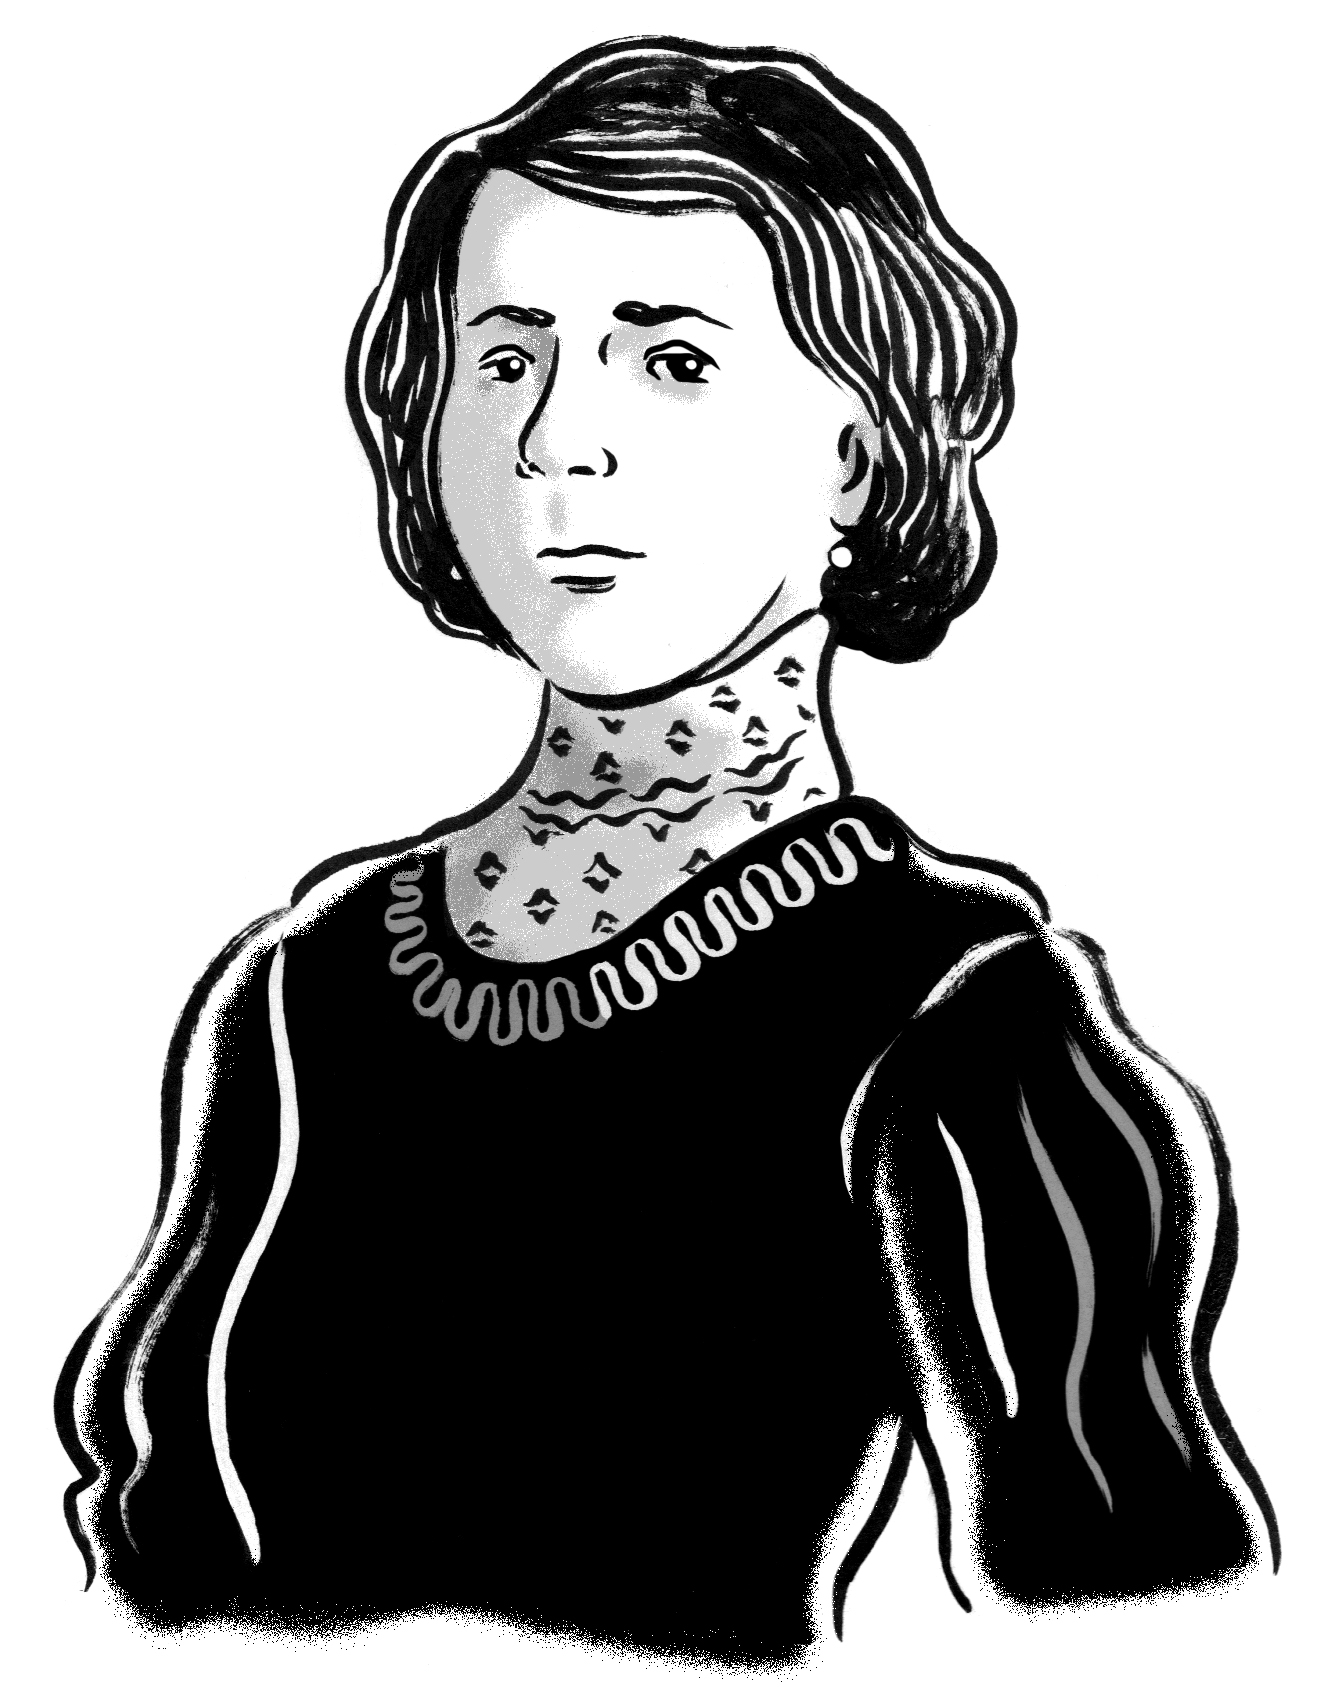
\includegraphics[width=6cm]{./imgs/autor10.jpg}
\end{center}


\chapter{A prova}

A mãe deu a bênção a Nátotchka\footnote{Nátochka é diminutivo de
  Nata, apelido de Natália.} e a mandou dormir\ldots{}

Magricela, de cabelos escuros e olhos grandes e algo assustados, Nata ou
Marmotinha, como papai a chamava, de brincadeira, devido ao rostinho
vivo de nariz arrebitado, correu rapidamente para o quarto das crianças.

A janela do quarto estava escancarada. Perto das camas de Nata e
Variucha --- sua irmã mais nova, de oito anos ---, a criada Sacha
trabalhava:

--- Sacha, eu mesma faço a cama! --- disse Nátochka. --- Pode ir\ldots{}
Também vou trocar Variucha\ldots{} Enquanto ela está sendo penteada no quarto
da mamãe, vou estudar um pouco para a prova de amanhã\ldots{} Não me
perturbe\ldots{}

Sacha inclinou a cabeça, sinalizando que entendera a patroa, e saiu\ldots{}
Embora fosse a empregada e nunca tivesse estudado, sabia muito bem o que
era uma prova.

Prova é uma coisa terrível, uma coisa monstruosa, que assusta de forma
indizível as pobres crianças que estudam. A prova manifesta"-se ora como
uma bruxa terrível, que traz lágrimas e pesar, ora como uma feiticeira
alegre, que dá uma felicidade grande\ldots{} Nátotchka pensava
involuntariamente em quem se manifestaria na prova de geografia do dia
seguinte --- a bruxa terrível ou a feiticeira boa\ldots{}

Macieiras estendiam"-se à janela do quarto das crianças\ldots{} Suas flores
brancas, de um perfume inebriante, eram tão bonitas! Nátotchka esticou a
mão, arrancou uma e cheirou longamente o aroma maravilhoso, suave e ao
mesmo tempo picante.

Como estava agradável agora na aldeia\ldots{} Na chácara Nedálny, bonita e
aconchegante, para onde iriam, logo depois da prova, a mãe, o pai, a
avó, ela e Variucha\ldots{}

Logo depois da prova\ldots{}

A prova!

O corpo inteiro de Nátotchka tremeu\ldots{}

Prova de geografia\ldots{}

A mais terrível, a mais desagradável\ldots{}

Fazia três dias que se preparava para ela, esforçando"-se para enfiar em
sua cabeça de menina rios, montes, lagos, toda uma rede ardilosamente
tecida dos mais variados nomes e denominações\ldots{}


Nátotchka revisou quase tudo o que era necessário\ldots{} Faltava apenas um
ponto\ldots{} O último\ldots{} O ponto das ilhas\ldots{} O mais terrível, o mais
insuportável. Ela tinha reservado a tarde para revisá"-lo, mas não fez
nada\ldots{} Primeiro, ficou brincando no balanço do pátio com Avdiuchka, o
filho do caseiro\ldots{} Depois, ensinou Fru"-Fru, uma galga italiana, a andar
nas patas traseiras\ldots{} Depois, em casa, discutiu com Variucha\ldots{}
Por que ela mesmo não se lembrava agora.

No fim das contas, ficou sem estudar o ponto --- o mais terrível!

Teria que revisá"-lo à noite\ldots{} Custasse o que custasse, Nátotchka tinha
que decorá"-lo; era a primeira aluna da classe e não podia de jeito
nenhum ``fazer feio'' na frente das amigas.

Além do mais, a moreninha Kátia Vanítskaia mirava ocupar o lugar dela.

Kátia tinha notas boas, mas um pouco piores do que a rival.

Nata ia bem nos estudos. Muito bem, aliás\ldots{} Só a geografia\ldots{}

Geografia insuportável! Em geografia, Nátotchka tirava 7, quando era
possível tirar 10.

Ela sentou"-se no parapeito da janela, abriu o livro e começou a estudar.

--- Sumatra\ldots{} Java\ldots{} Bornéu e Celebes! Sumatra\ldots{} Java\ldots{} Bornéu e
Celebes! Celebes! Celebes! Celebes!

E, de repente, um riso maroto percorreu os lábios da menina.

--- A ilha Celebes e o professor Seles\ldots{}

Um nome terrivelmente ridículo!\ldots{} O professor de geografia deu de se
chamar Seles\ldots{} E Celebes\ldots{}

Nátotchka não concluiu seu pensamento, pois, nesse instante, Variucha, a
irmã mais nova, entrou feito um furacão no quarto e, sacudindo os
cabelos cacheados, gritou:

--- Nata! Nata! Desabotoe meu vestido atrás\ldots{} Você mandou Sacha embora
e sozinha eu não consigo.

Nátotchka desabotoou, repetindo:

--- Sumatra\ldots{} Java\ldots{} Bornéu e Seles\ldots{} Não, Celebes\ldots{} Celebes\ldots{}
Celebes\ldots{} Celebes\ldots{}

--- Nata, o que é que você está resmungando aí? --- quis se informar a
curiosa Variucha, com os olhinhos ligeiros cintilando.

--- Calada! Tenho prova --- observou Nata com ar de importância\ldots{}
Compenetrou"-se imediatamente. Sua carinha ficou séria\ldots{}

Prova, oh! Um assunto sério.

Variucha trocou"-se em profundo silêncio, tentando não distrair a irmã de
jeito nenhum.

Nátotchka fitava a janela com os olhos grandes e algo assustados e
sussurrava:

--- Sumatra\ldots{} Java\ldots{} Java\ldots{} Java\ldots{} Sumatra\ldots{}

--- Nátotchka! --- soou a voz tímida de Variucha\ldots{} --- Fecha a janela?
Está ventando\ldots{}

Nata bateu a janela, irritada, sem parar de sussurrar\ldots{}

Variucha no começo prestou atenção no sussurro da irmã, depois seus
olhinhos começaram a se fechar.

--- Nátotchka! --- disse quase dormindo, mal movendo a língua. --- E
essa prova é muito difícil?

\begin{figure}%[ht!]
\vspace*{-2.1cm}
\hspace*{-2.2cm}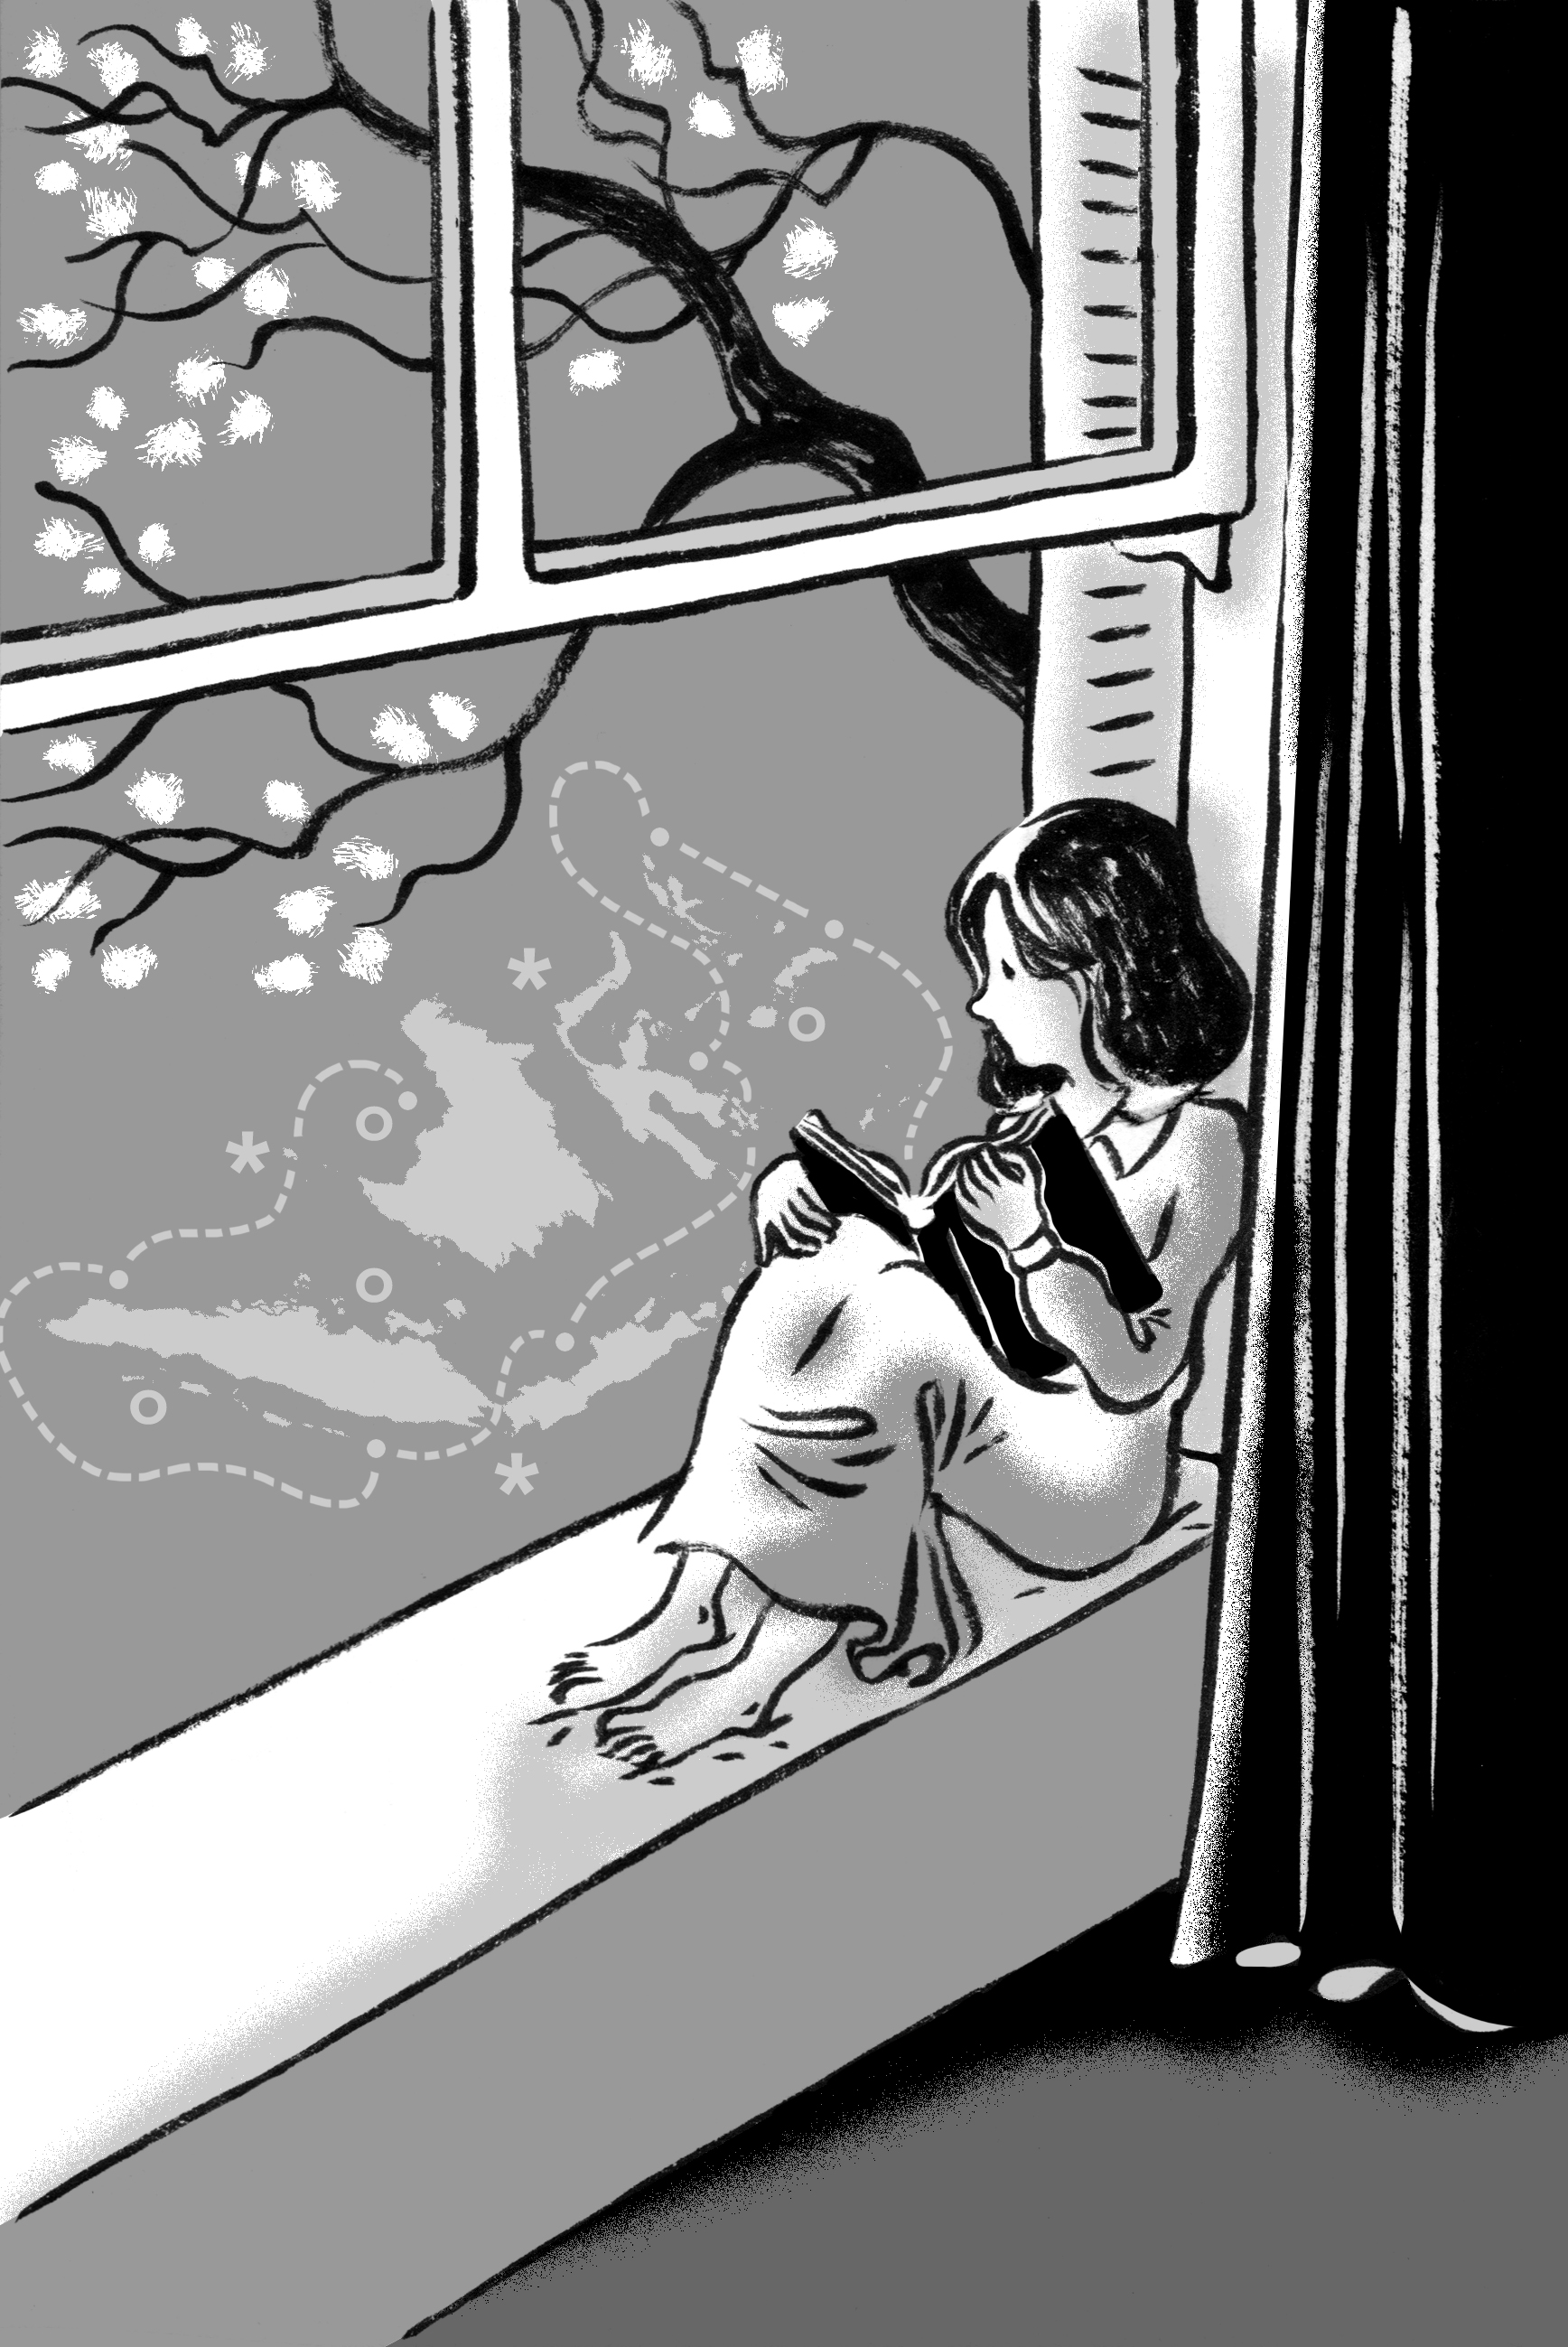
\includegraphics{./imgs/cena12.jpg}
\end{figure}

--- Ã"-hã! --- emitiu Nátotchka e, sentada no peitoril da janela, começou
a resmungar algo com determinação, olhando esporadicamente para o livro.

Aos poucos, a casa inteira silenciava.

Variucha dormia havia tempos, com a mãozinha debaixo da bochecha.
Felizarda, não tinha uma prova pela frente!

Nátotchka decorava com mais empenho:

--- Quios\ldots{} Samos\ldots{} Lesbos\ldots{} Quios\ldots{} Samos\ldots{} Lesbos\ldots{}

--- Deus! Os, os, que osso --- gracejou a moça,
amargurada, e voltou a olhar para o manual.

Ao longe, no corredor, o relógio bateu\ldots{}

Nátotchka contou as batidas\ldots{} Onze em ponto! Ah, como o tempo corre!

E que vontade de dormir! Os olhinhos se fechavam. Ela pôs"-se a
sussurrar, ainda mais insistente:

--- Quios\ldots{} Samos\ldots{} Lesbos\ldots{}

Finalmente, as ilhas do arquipélago grego estavam decoradas\ldots{} Nátotchka
recomeçou com Sumatra, Bornéu, Java e Celebes.

Oh, que horror!

Sumatra, Java e Bornéu foram esquecidas\ldots{}

Que dirá de Celebes!

Nátotchka comprimiu os lábios e, prestes a chorar, retomou seus
sussurros. E suas pálpebras pesavam, pesavam\ldots{} As ideias se
embaralhavam na cabeça\ldots{} A noite branca\footnote{Em Petersburgo, são
  chamadas ``noites brancas'' as que não escurecem durante alguns dias no verão, principalmente em junho.} de maio inspirava devaneios\ldots{} E
Nátotchka adormeceu; contra a vontade e a expectativa, adormeceu no
peitoril largo da janela. Sua mãe entrou no quarto e viu a filha
dormindo.

--- Pobre menina! Ah, essas provas! --- disse, aflita, em sua mente, e,
chamando Sacha baixinho, acomodou com ajuda dela Nátotchka na cama.

Ao dormir, a menina balbuciava algo\ldots{} Talvez uma ilha, talvez um rio\ldots{}

Teve um sonho estranho nessa noite\ldots{}

Sonhou com Bornéu, Sumatra, Java e Celebes.

Bornéu na forma de um almofadinha magricela, de cartola alta e
pincenê\ldots{} Sumatra na forma de uma vendedora gorda de maçãs à porta da
igreja\ldots{} Java tinha o rosto e os cabelos da irmã, Variucha\ldots{} E Celebes
era o próprio Seles\ldots{} O professor de geografia, um velhinho grisalho e
bilioso\ldots{}

Ele olhava para Nata, ameaçava"-a com o dedo de unha amarela e estreita,
e dizia com voz sibilante:

--- Quios, Samos e Lesbos ficam muito gostosas com canela e creme\ldots{} Mas
vou lhe dar nota 1 assim mesmo, cara senhorita!

E Nátotchka, aflita, ficou petrificada \ldots{}

\asterisc

--- Dártseva, você estudou todos os pontos? --- a moreninha Vanítskaia
recebeu Nátotchka na porta da classe com um sorriso maroto.

Havia confusão no rosto de Nátotchka.

Não sabia o último ponto, o das malditas ilhas.

Ela mesma não lembrava como adormecera à noite, e Sacha a acordou pela
manhã com dificuldade\ldots{} Por pouco a menina não chegou ao colégio
atrasada.

Vanítskaia estudara tudo e parecia muito satisfeita consigo mesma.

Já Nátotchka não queria reconhecer que não sabia o último ponto\ldots{} E, em
resposta à outra, acenou positivamente com a cabeça em silêncio.

Às dez em ponto, entraram na classe o terrível Seles, a diretora do
colégio e mais um velhote\ldots{} Diziam que era professor de outro colégio
e, como se não bastasse, muito severo. Todos os três se sentaram à mesa
verde e a prova começou.

Para a prova oral, as meninas eram chamadas à mesa de cinco em cinco\ldots{}
Primeiro as más alunas, depois as boas.

Nátotchka sabia que ela e Vanítskaia seriam chamadas por último.

E os bilhetes com os pontos iam desaparecendo da mesa. Os melhores, os
que Nátotchka poderia responder de forma excelente, foram os primeiros a
serem sorteados.

Finalmente, quase toda a classe fora arguida.

--- Senhoritas Vanítskaia e Dártseva? --- soou a voz do professor.

Nátotchka levantou"-se como que em delírio\ldots{} Lembrava"-se muito bem de
que nenhuma das meninas tinha respondido sobre as ``terríveis'' ilhas
\ldots{} Devia ser o último ponto a cair na prova.

Lançou um olhar rápido sobre a mesa verde.

Lá havia apenas dois pontos para sortear\ldots{} Um deles era certamente
esse.

Nátotchka sabia disso.

--- Bornéu\ldots{} Java\ldots{} Sumatra\ldots{} Celebes!\ldots{} --- proferiu seu cérebro,
em turbilhão, e ela esticou a mão.

Vanítskaia pegou um ponto\ldots{} Nátotchka o outro.

--- Ah! --- e um rubor se irradiou pelas faces dela.

Tinha diante de si o maldito último ponto.

``Horror! Horror!'', passou"-lhe pela cabeça.

A aldeia\ldots{} O verão bom e alegre, as férias felizes\ldots{} Estava tudo
perdido!

O desespero sufocava Nátotchka\ldots{} Círculos pretos rodopiavam diante de
seus olhos\ldots{} A cabeça girava\ldots{} Mal se aguentava nas pernas\ldots{}

Vanítskaia respondeu primeiro\ldots{} Tinha um ponto fácil, os rios da
Rússia. Nátotchka sabia"-o como o Pai Nosso\ldots{} Ah, se ela tivesse ficado
com esse ponto. Oh, Senhor! Por que o destino era tão injusto com ela?

Kátia Vanítskaia respondeu seu ponto com desenvoltura.

--- O Volga\ldots{} Os afluentes do Volga\ldots{} Kama e Oká --- assinalava em voz
alta, deslizando o ponteiro pelo mapa pendurado na parede ---, os
afluentes do Kama\ldots{}

--- Pare! Pare! --- o professor de geografia interrompeu a menina\ldots{} ---
A senhorita está careca de saber de tudo isso\ldots{} Tem que saber muitas
outras coisas\ldots{} Para a senhorita e para Dártseva, as melhores alunas,
eu coloco mais exigências, por isso troque agora de ponto com sua
colega. Responda o ponto de Dártseva\ldots{} Dártseva, responda a senhorita
sobre os rios da Rússia\ldots{}

O que era aquilo? Será que Nátotchka tinha ouvido mal?

Não! Não! Vanítskaia já estava lhe estendendo a mão e pegando o bilhete
dela.

Vanítskaia estava tranquila. Seu rosto resplandecia. Conhecia as ilhas
ainda melhor do que os rios. E respondeu lindamente\ldots{} Tirou nota 10 e
foi mandada para seu lugar com um elogio.

Nátotchka pegou o ponteiro com desenvoltura e moveu"-o pelo mapa\ldots{}

Uma chuva de nomes e denominações\ldots{} Uma enxurrada deles jorrava de seus
lábios.

Estava fora de si de felicidade e jogava o corpo para a frente como se
tivesse asas.

--- Formidável! Formidável! --- elogiou"-a o professor. --- A primeira
aluna mostrou seu melhor lado.

--- Querido, querido Celebes! --- respondeu Nátotchka mentalmente, com
vontade de se lançar ao pescoço do professor, que não desconfiava de
nada, e de enchê"-lo de beijinhos\ldots{}

Nata tirou nota máxima. A prova terminou.

Fora de si de felicidade, Nátotchka voou para casa.

--- Passei! --- gritou como uma possessa, irrompendo na sala de visitas
feito um furacão.

De susto pela aparição ruidosa da filha, a mãe deixou cair o trabalho
que tinha nas mãos.

--- Sacha, passei\ldots{} Quios\ldots{} Samos\ldots{} Sumatra, passei em tudo ---
Nátotchka continuou a gritar, correndo para o cubículo da criada Sacha.

--- Variucha! Variucha! --- num segundo sua vozinha sonora propagou"-se
pelo corredor. --- Venha logo, passei na prova!

Um minuto depois, a casa inteira sabia que as insuportáveis ilhas de
Sumatra e Java não tinham aprontado para Nátotchka e que no mundo não
havia melhor professor que Seles\ldots{}

\medskip

{\footnotesize\hfill\emph{Tradução: Irineu Franco Perpetuo.}}

\chapter{A mãe}\label{part13}

Тoc"-toc! --- a máquina incansável soa a noite inteira.

Uma tira longa de chita farfalha e range, ou uma fazenda barata de lã
desliza suavemente da mesa de trabalho para o chão.

Toc"-toc! --- os sons familiares formam uma melodia regular.

A mãe, inclinando as costas arqueadas (pouco tempo atrás tão eretas e
aprumadas) sobre o trabalho, girava a roda da máquina de costura com uma
mão, ajeitando o trabalho com a outra.

A cama de Volódia\footnote{Volódia, apelido de Vladímir.} fica
exatamente contra a porta. Quando acorda à noite, sempre vê o quadro
conhecido. A mesa atulhada de trabalho, a máquina de costura e, diante
dela, a figura cansada e arqueada de sua mãe, o rosto pálido com
cavidades circulares azuis em torno dos olhos, a doce cabeça grisalha e
os lábios tristemente comprimidos, que de uns tempos para cá
desaprenderam completamente a sorrir. Volódia lembra com clareza desde
quando.

Desde o momento em que, na cama larga, no lugar de um pai vivo, surgira
um homem estranho e morto que, para Volódia, a irmã mais velha e o
irmãozinho caçula, pouco lembrava o pai alegre e bondoso que com gosto
ganhava de Volódia no jogo de damas ou desenhava caricaturas divertidas
no álbum; desde o dia da morte do pai, a mãe desaprendera a sorrir.
Desde então, Volódia só podia imaginá"-la ao trabalho, costurando
vestidos baratos de lã e de chita para a população feminina mais pobre
do prédio ou para as criadas dos outros. A mãe cobra tão pouco das
clientes que estas levam para costurar suas roupas despretensiosas de
muito bom grado.

Quando o pai estava vivo, ela não tinha que trabalhar dia e noite, noite
e dia. Ele era professor de desenho em três colégios. Não ganhava muito,
mas a pequena família não passava por apuros. Volódia e Chura\footnote{Chura,
  apelido de Aleksandra.} estudavam em um colégio à custa do Estado e
quem ensinava o alfabeto e a formação das sílabas ao caçula,
Lionka,\footnote{Lionka, apelido de Leonid.} era a mãe. Aliás, ela
também ajudava Chura e Volódia, especialmente nas línguas estrangeiras
(eles tinham dificuldade para línguas).

\begin{figure}%[ht!]
\vspace*{-2cm}
\hspace*{-2.4cm}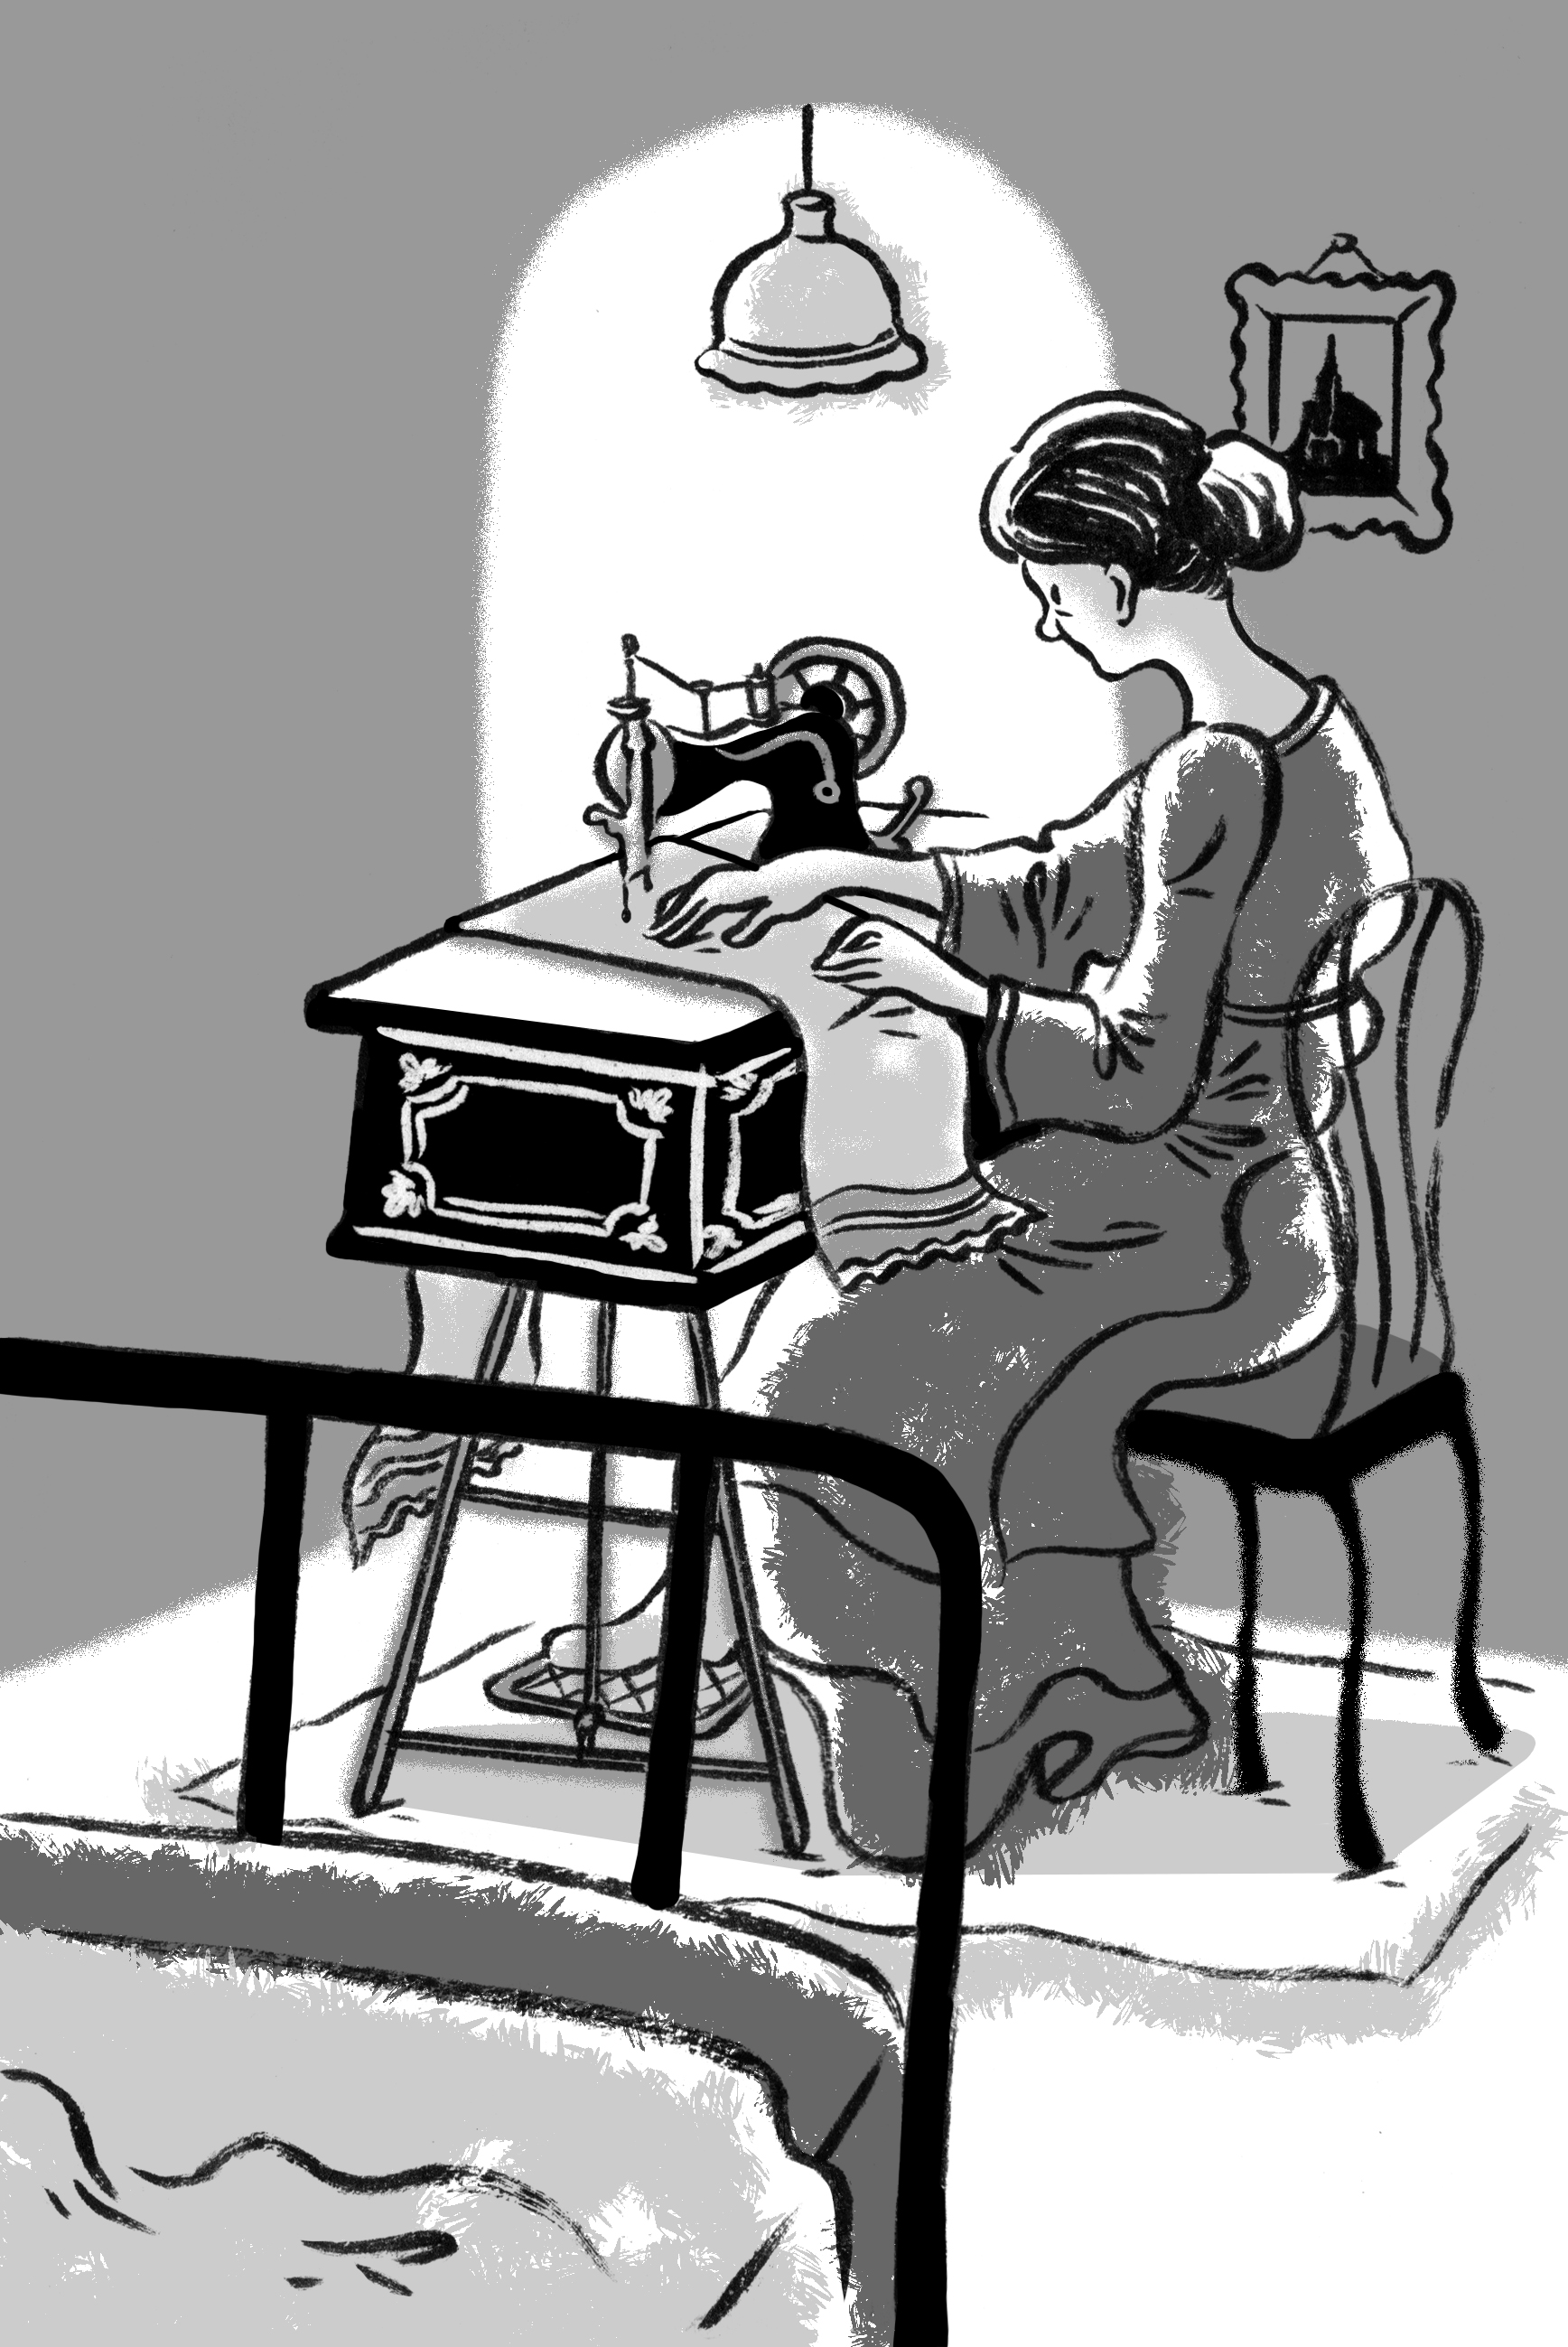
\includegraphics{./imgs/cena13.jpg}
\end{figure}

Mesmo agora, ela ajuda com frequência Volódia e Chura nas lições de
francês e de alemão. E, de vez em quando (é preciso reconhecer!),
Volódia recorre a seu auxílio para estudar matemática e outras matérias.

A mãe é talentosa. Podia também dar aulas, mas não tem vontade. Prefere
pegar encomendas de costura e trabalhar encurvada a sair de casa e
correr atrás de aulas.

--- Deus sabe o que pode acontecer com as crianças sem cuidados --- diz
ela quando pessoas boas lhe oferecem aulas. --- Meu Lionka ainda é
pequeno, tem sete anos. E os mais velhos não estão muito longe. Chura
tem catorze, Volódia onze. Onde é que já se viu largar sozinhas crianças
tão pequenas?

Volódia discorda da mãe com a maior sinceridade. Por exemplo, por acaso
ele é pequeno? Com prazer navegaria pela América, vagaria por pradarias
e lutaria com índios, como o Desbravador.\footnote{Alusão ao romance
  \emph{O desbravador} (1840), do norte"-americano James Fenimore Cooper
  (1789--1951).} Alguém pequeno seria capaz disso? Oh, claro que sua mãe
se enganou. Ele, Volódia, era um perfeito adulto.

E uma noite o adulto fez sua existência ser lembrada com um gritinho.

--- Volódia! Não está dormindo, meu bem? O que você tem, queridinho? ---
ela levantou"-se do lugar, aflita, e apressou"-se na direção do
``queridinho'', saindo da antessala, o quarto minúsculo em que
trabalhava à noite, com medo de incomodar os outros filhos.

O apartamento deles se resume em um quarto e uma cozinha. E por tal
moradia são obrigados a pagar dezesseis rublos. Sem exagero! Dezesseis
rublos!

Volódia ficou feliz ao ver a mãe ao seu lado e, ao mesmo tempo,
envergonhado por tê"-la assustado e afligido.

--- Você só sabe trabalhar --- disse com voz fingidamente sonolenta,
pegando ainda no alto a mão esquerda da mãe, magra, com o dedo indicador
picado de agulha. E, falando mais baixo, com uma vozinha culpada,
acrescentou: --- Deveria se deitar, mãezinha\ldots{} Mas fica trabalhando
enquanto nós dormimos\ldots{}

--- Durma, durma, queridinho! --- secundou a mãe com uma ponta de
alegria na voz. --- Graças a Deus, você pode dormir. Na sua idade, o
sono é tudo! Eu vou ficar trabalhando mais um pouco\ldots{} Sobrou um
tiquinho para costurar.

Volódia conhece esse ``tiquinho''. Sobrara para costurar o corpete
inteiro da vizinha, uma cozinheira gorda.

A pobre mãe ficaria trabalhando de novo até o amanhecer!

O menino sentiu um nó na garganta. Fez um biquinho com os lábios, deu
uma beijoca na palma da mãe e despencou de bruços no travesseiro,
tentando esconder nos olhos semicerrados as lágrimas que traíam seu amor
e sua enorme compaixão.

E a mãe cuidadosamente enfiou embaixo dele o cobertor, como um
``saquinho'', e o beijou com ternura. Depois ela agasalhou Lionka, que
murmurou algo dormindo --- ele se descobrira desordenadamente e
derrubara o cobertor no chão. Finalmente a mãe se aproximou da Chura,
que divide uma cama larga com ela. Depois voltou a seu cubículo, na
antessala, e até o amanhecer, sem erguer as costas, acionou a máquina a
cujo ruído estavam habituadas as crianças, que dormiam profundamente sob
o som monótono.

\asterisc

Nesse dia Volódia voltou do colégio mais cedo do que de hábito. A cabeça
lhe doía e ele sentia o corpo todo quebrado. Não conseguira ficar na
aula e foi para casa. A mãe, aflita por seu menino, correu para ajudá"-lo
a se trocar, depois requentou no fogareiro a sopa da véspera e um
bolinho de carne.

Mas Volódia não podia nem pensar em comer. A cabeça girava e, diante dos
olhos, alastravam"-se círculos escuros. Gotas de suor imediatamente
surgiram na testa dele.

--- Só não fique doente, só não fique doente, meu anjo --- ela
sussurrava, angustiada, beijando seu menino com ternura.

Pois foi justo o que aconteceu: Volódia ficou doente\ldots{} E não só
Volódia, como também Chura e Lionka.

Os filhos de Beriózova estavam com sarampo.

A pobre Mária Ivánovna perdeu a cabeça no primeiro minuto de seu
infortúnio. Com essa doença terrível, entraram no apartamento minúsculo
três hóspedes indesejados: o aumento dos gastos, a impossibilidade de
trabalhar e a necessidade.

Agora a máquina não soava mais --- as clientes, assustadas com o
sarampo, tinham medo de fazer encomendas. A mãe corria pelas três camas,
dividia"-se igualmente entre seus três pacientes preciosos.

--- Mamãe, tenho sede! Quero beber! --- delirando de calor, chiou Chura,
que aguenta mal qualquer doença, que dirá o sarampo.

E a mãe levava à filha doente limonada fresca quente.

--- Beba, minha querida, beba! --- dizia erguendo do travesseiro, com as
mãos ternas, a cabeça loira da sua mocinha.

Chura provava a bebida, fazia uma careta e chiava:

--- Ui, que porcaria! Está quente! Parece chá! Mas eu queria geladinha e
azedinha\ldots{} Não tem limão aqui, mamãe!

--- Gelada não pode, filhinha, o médico proibiu!

--- Mas eu quero! --- continuou Chura, caprichosa, pronta a se desfazer
em lágrimas.

Volódia não podia suportar a pomada viscosa que tinham mandado esfregar
nas crianças. Dava"-lhe náuseas. E nele o processo da doença era mais
intenso que nos irmãos. A mãe fitava seu rostinho magro com angústia, ao
passo que o rosto dela estava amarelo e pálido de medo.

--- Volódia, meu bem, você não se sente bem? --- perguntava de forma
quase inaudível.

Daí Lionka desatou a chorar. Tinha quebrado a cabeça de um soldadinho de
chumbo, abriu um berreiro e exigia ostensivamente a mãe.

O médico chegou na hora certa. Deu palmadinhas nas crianças,
auscultou"-as, prescreveu remédios. A mãe novamente saiu atrás deles. Não
havia ninguém que pudesse ir em seu lugar. Não tinha empregada. Ela é
que preparava a canja, alimentava os três de colher, passava a noite
inteira ao pé de suas camas, sem piscar o olho. Mal as crianças
adormeciam, tirava o crochê interrompido do bolso e fazia renda a noite
inteira. A renda, quando estivesse pronta, podia ser lavada, sem ter
contágio de sarampo. E se vendia bem na feira.

Sempre e em toda parte lá estava ela. Precisava estar. Era a única
trabalhadora da família. As crianças eram pequenas. Tinham que ser
curadas, colocadas de pé. Ela tinha que estar pronta para o trabalho.
Não podia ser de outra maneira. Ela era a mãe.

\asterisc

O sarampo, felizmente, não foi perigoso. As crianças se salvaram. Todas
as três. Mária Ivánovna recobrou o ânimo. Além disso, conseguiu mandar
os dois mais velhos, graças a um empenho redobrado, a uma
\emph{datcha} do Estado para passar o verão. E Lionka foi enviado, por
uma quantia, para a aldeia de conhecidos.

As clientes voltaram a aparecer. A máquina de novo soava dia e noite.
Também era preciso costurar roupas novas para os filhos. Era
desconfortável, ficariam na companhia de pessoas\ldots{} Não queria que
rissem deles. Deus nos livre. Não são órfãos. Têm mãe!

E as crianças já faziam planos para o esperado verão, agitadas,
contentes, sonhadoras. Estavam felizes por irem à \emph{datcha} pela
primeira vez após a morte do pai! Veriam o bosque, o campo, o rio\ldots{}
Iriam colher frutinhas silvestres, cogumelos, pescar\ldots{} E tudo por causa
do sarampo, bendito e querido sarampo!

A mãe foi deixar seus filhos mais velhos na plataforma da estação
ferroviária (Lionka tinha sido levado à aldeia uma semana antes). Lá
repentinamente saltou aos olhos de Volódia a mudança ocorrida com ela
nos últimos tempos: sua figura esquálida, o rosto cansado e atribulado.

E, pela primeira vez, passou tal pensamento pela cabeça do menino
contente com a viagem e com o verão agradável que teria pela frente:

--- Como a pobre mamãe está cansada e magra\ldots{} Enquanto nós, egoístas,
vamos partir sem remorso\ldots{}

O coração apertou\ldots{} Uma dor aguda. Volódia quis se lançar na direção da
mãe, pronto para dizer que ficaria com ela em casa, para consolá"-la,
para partilhar de sua solidão, mas\ldots{} O terceiro apito soou\ldots{} O trem se
pôs em marcha, e a mãe mal conseguiu dar a bênção aos filhos e saltar do
vagão. Eles partiram\ldots{}

\medskip

{\footnotesize\hfill\emph{Tradução: Irineu Franco Perpetuo.}}


\chapter*{}
\label{part14}
\thispagestyle{empty}

\begin{vplace}[1.5]
{\HUGES\hfill\textbl{SACHA TCHÓRNY}}

{\LARGE\hfill\textlt(1880–1932)}
\end{vplace}

\pagebreak
\thispagestyle{empty}
\mbox{}
\vfill
\begin{center}
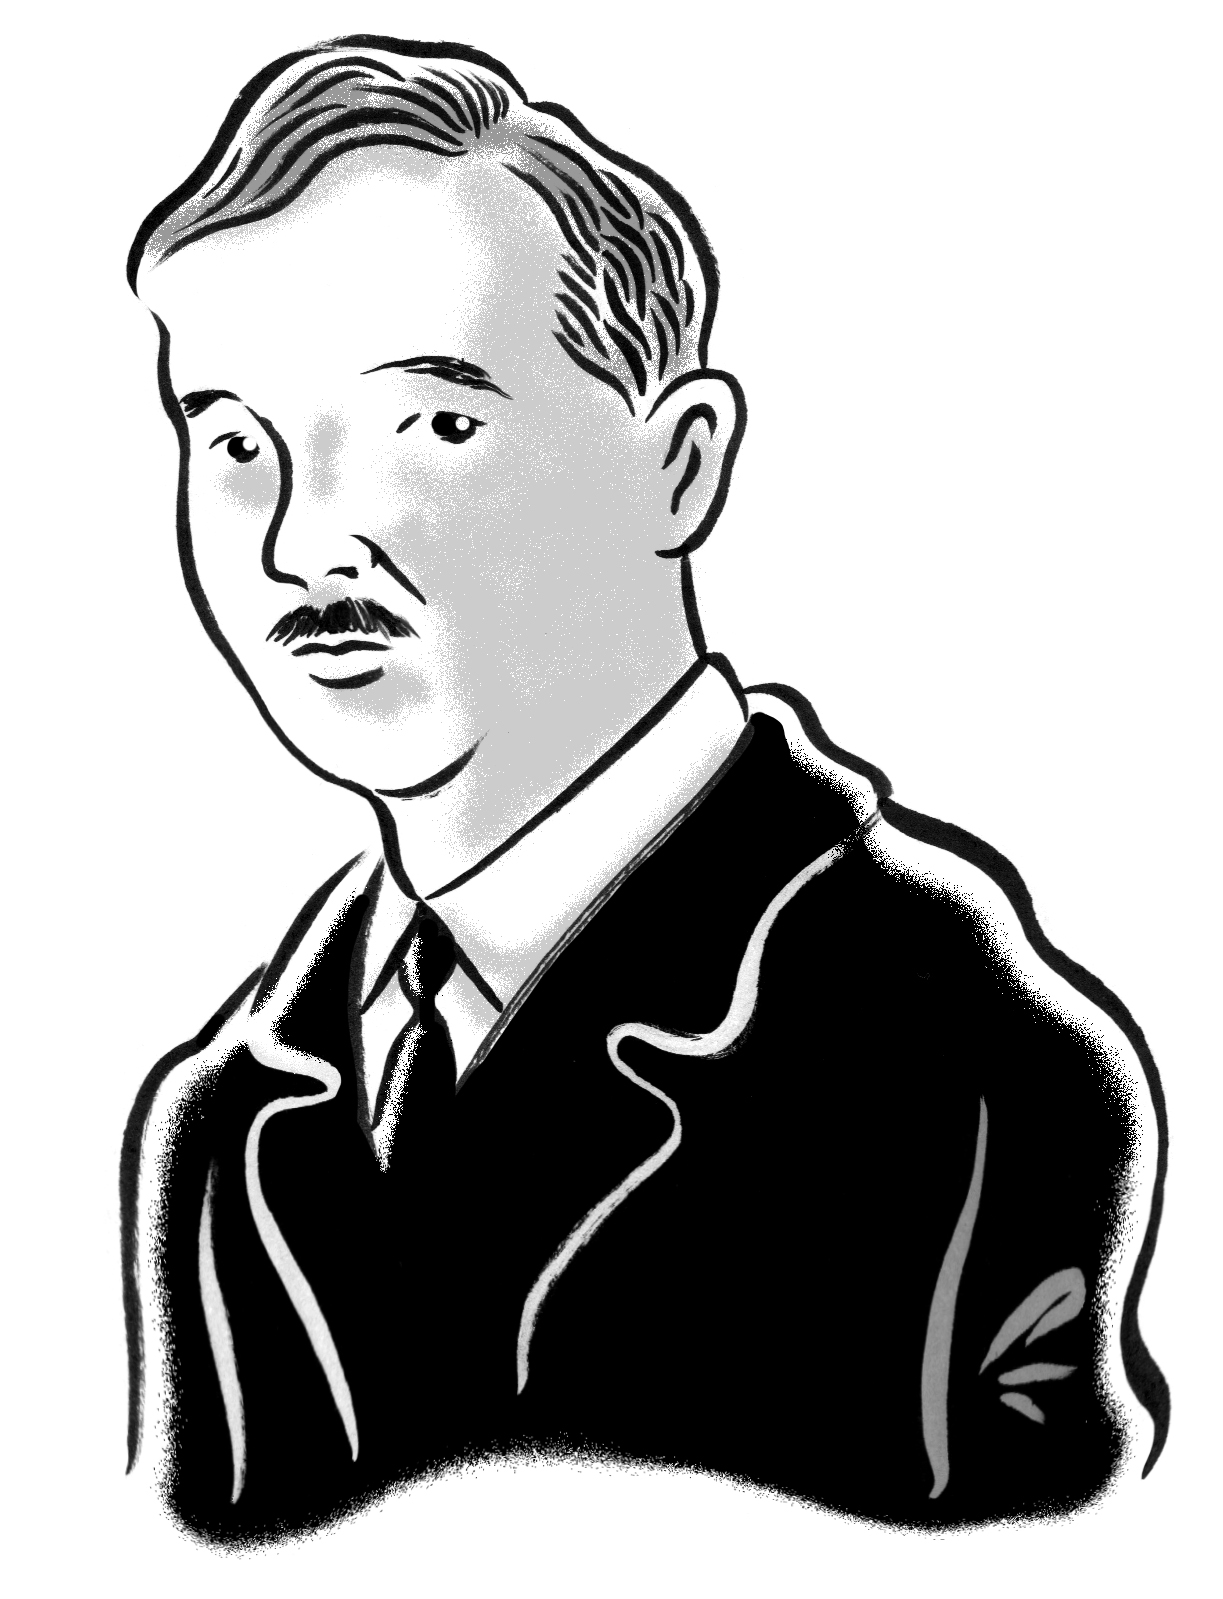
\includegraphics[width=6cm]{./imgs/autor11.jpg}
\end{center}

\chapter{A pedrinha vermelha}

A \emph{datcha} ficava junto à floresta. Jórjik tomou café rapidamente e
correu para os canteiros. Na véspera ele e o caseiro tinham plantado
ervilha --- era preciso ver se ela já havia brotado. Mas ali ainda não
havia nada. Jórjik remexeu na terra com ajuda de um graveto, tirou um
grãozinho de ervilha e enterrou"-o de novo.

Depois, ele se aproximou da cerca e começou a olhar a floresta: abetos
balançavam atrás de arbustos, água brilhava num rego, dois corvos
passeavam solenemente debaixo de um junípero e conversavam entre si.

``Vou para a floresta'', pensou Jórjik. ``Mas andarei somente um pouco,
até aquela betulazinha\ldots{}''

Pensou e pôs"-se a caminho. Uma tábua estava completamente caída na velha
cerca e passar pela fresta não seria difícil: primeiro um pé, depois a
cabeça, depois o outro pé --- e lá estava a floresta.

No caminho para a bétula, Jórjik se virou duas vezes: ``Lá está ela, a
nossa \emph{datcha}\ldots{} O telhado vermelho, e"-nor"-me, com um pombo
sentado em cima\ldots{}''. Dali também podia ver a fresta na cerca.

O menino chegou até a pequena bétula e sentou para descansar. ``Ficarei
um bocadinho antes de ir para casa. Salve, besouro! Por que está se
arrastando pelo meu joelho?''

Ele tirou o besouro, colocou"-o sobre o musgo e disse:

--- Fique aqui, senão vai se perder no caminho!

Jórjik olhou ao redor: pequenos abetos estavam rangendo (``eles devem
ter um apito no meio, como o meu coelho'', pensava ele); uma atrás da
outra formigas corriam com pedacinhos de madeira para algum lugar, como
se fossem um fiozinho preto vivo; samambaias faziam reverência; nuvens
de chuva pairavam alto --- para Jórjik uma delas lembrava o caseiro: de
barba branca e cachimbo na boca. O dia estava claro e nada ameaçador\ldots{}

--- Ah, que desgraça! --- de repente alguém pipilou na floresta.

Jórjik se assustou e deu um salto:

--- Qual desgraça? Quem está me assustando?

--- Ei! Ajude"-me, querido! --- de novo alguém falou atrás dos arbustos.

O menino quis chorar e correr em disparada para casa, mas em seguida ficou
envergonhado. A voz era fina e queixosa, igual à da Amichka quando lhe
prendiam o rabo. Por que teria medo? Era bem grandinho, afinal\ldots{} Talvez
a menina da \emph{datcha} vizinha tivesse se perdido --- seria preciso
pegá"-la pela mão e levá"-la de volta.

--- Quem está choramingando aí? --- Jórjik perguntou corajosamente.

--- Sou eu, uma ve"-lhi"-nha\ldots{} Venha para cá, menino!

--- Mas onde está, tia? --- perguntou ele e olhou em volta. Não podia
ver a velhinha em lugar algum.

--- Aqui, atrás do rego. Aí mesmo, mais à esquerda!

Jórjik se aproximou do rego e passou para o outro lado através de um
abeto que havia se quebrado.

Sobre um montículo de terra estava deitada uma velha franzina usando um
casaquinho azul. Suas pernas caíram no pântano e não havia jeito de
tirá"-las de lá: por mais que as puxasse, elas se afundavam mais e mais.
Era como uma mosca em um pires com geleia, sem tirar nem pôr.

Jórjik achou graça nisso, mas se conteve: a velha poderia zangar"-se com
ele --- de repente é um tipo de feiticeira?

--- Tia --- disse ele ---, dê cá a sua mão, eu vou tirá"-la daí!

--- Não dará conta! Suas mãos são muito curtas e você deve ter a força
de uma barata. Olhe para lá! Debaixo da bétula está a minha trouxa.
Pegue a corda dentro\ldots{} Amarre uma ponta dela à bétula e a outra jogue
para mim. Assim, menino esperto\ldots{} Vamos lá, muito bem!

A velhinha, dando grasnidos, se agarrou à corda, então gritou com voz
rouca e, toda vermelha, tirou as pernas do pântano. Depois de limpar"-se
e sacudir"-se sobre um montículo, ela disse a Jórjik:

--- Obrigado, meu jovem! Ah, que pernas redondinhas você tem! O que
posso lhe dar como recompensa por ter me tirado de lá?

O menino caiu em reflexão.

--- Dê um camelo. Um pe"-que"-ni"-no!

--- Quá"-quá! Um camelo\ldots{} Que menino original\ldots{} Onde é que eu
arranjaria um camelo para você? E, vamos e venhamos, na sua casa ficaria
apertado para ele; o bicho também estragaria os canteiros\ldots{} Espere! ---
disse a velha. Ela encostou a mão no ouvido e olhou para cima.

--- Para onde está olhando, tia? --- perguntou Jórjik.

--- Os corvos estão dizendo para eu sair daqui. Eles enterraram debaixo
da bétula um ossinho, querem pegá"-lo e nós estamos atrapalhando\ldots{} Está
bem, agora mesmo iremos!

--- Veja só! --- gritou Jórjik. --- Como é que sabe que estão falando
sobre o osso?

--- Eu sei, quá"-quá\ldots{} Está vendo, amiguinho? --- a velha tirou do
ouvido uma pedrinha vermelha e a mostrou a Jórjik. --- É uma coisinha à
toa, mas está tudo aí. Basta colocá"-la no ouvido para que escute como
conversam os corvos, as vacas, os mais variados insetos\ldots{}

--- Verdade? E como o elefante fala, também se pode escutar?

--- Tanto faz, que seja um elefante\ldots{} Só que aqui não há elefantes\ldots{}

--- Tia! --- disse Jórjik e agarrou a velha pelo casaquinho. --- Você
perguntou o que me dar por tê"-la tirado do pântano. Dê essa pedrinha.
Vá, por favor.

A velhinha pendurou a trouxa nas costas, acariciou a mão de Jórjik e
riu:

--- Ora essa, que pidão. Veja o que deu de escolher! E eu ficarei com o
quê? Estar na floresta sem esta pedrinha, meu querido, é o mesmo que uma
rã longe da água\ldots{} Não, peça outra coisa qualquer\ldots{}

--- Cara senhora! Dê por apenas um dia! Por um tempo\ldots{}

--- Não vai perdê"-la?

--- Por nada deste mundo!

--- E não a mostrará para ninguém?

--- Para ninguém! --- começou a pipilar Jórjik. --- Ah, isso será
divertido! Aqui tem a Amichka, tem o bode lelé, e"-nor"-me, maior até do
que você, sempre resmungando com seus botões, tem o galo, tem as
baratas\ldots{}

--- Calma lá\ldots{} --- disse a velha. --- Que pressa! Está bem. Pode ficar
com ela até de noite.

Ela enxaguou a pedrinha no rego, limpou"-a com um pano branco e a deu a
Jórjik.

--- Para a mamãe também é proibido mostrar? --- perguntou ele.

--- Para a mamãe pode\ldots{} Somente não diga como a conseguiu. É um
segredo. E de noite, quando for dormir, coloque a pedrinha sob o
travesseiro. Eu vou lá pegar.

--- Como vai lá? Amichka dorme no chão perto da minha cama --- assim que
a perceber, ela morderá você\ldots{}

--- Não morderá! Eu mesma posso morder quem quer que seja\ldots{} Então,
adeus, menino --- disse a velhinha. --- Calma, calma, fique parado aqui.

Ela colocou Jórjik com o rosto virado para a bétula.

--- Fique assim por um minuto e não se vire.

--- Já pode? --- perguntou Jórjik quando a velha tirou as mãos dele.

--- Ainda não.

--- E agora?

--- Agora pode! --- gritou a velhinha com a voz fina por trás dos
arbustos.

Jórjik se virou. A velha havia desaparecido. Na palma da mão dele estava
a pedrinha vermelha, miúda, miúda, do tamanho de uma joaninha. Ele
rapidamente a enfiou no ouvido, deu um salto e correu para casa.

Os dois corvos ainda passeavam debaixo do junípero. Jórjik se deteve:

--- Vamos lá, vamos lá!

Um corvo olhou de lado para o menino, virou"-se e crocitou:

--- Crás, é surpreendente! De novo esse menino. Crás, tão pequeno e
passeia sozinho pela floresta.

O outro corvo pensou e respondeu:

--- Crás, é estranho.

Jórjik caiu na risada, fez uma saudação afastando a perna e gritou:

--- Crás, senhores! Crás, queiram perdoar! Crás, mas não é da sua conta!

Meio minuto depois, ele já estava no jardim.

O jardim estava deserto. Apenas, em um atalho, um besouro grande marrom
revolvia terra. Ele fazia a sesta, aquecia as costas sob o sol e não
ouviu Jórjik se aproximar.

--- Zás! Peguei\ldots{} --- disse Jórjik, apanhou o besouro pelo peito e o
encostou no ouvido.

--- Zum"-zum"-zum, que aperto terrível\ldots{} --- zuniu o besouro. --- Com as
patas vou empurrar e com a barriga me esquivar, e logo me livro dessa\ldots{}
Zum"-zum"-ah!

--- Ai, faz cócegas! --- riu Jórjik e lançou o besouro para o alto.

O besouro voou e começou a cantar:

--- Zum"-zum"-zum, Jórjik está andando no atalho, e olhem só para mim!

--- Dacha! --- gritou Jórjik. --- Venha cá rápido!

--- Para quê?

--- Mostrarei uma coisa! Rápido!

De repente Jórjik lembrou que prometera à velhinha não mostrar a
pedrinha vermelha a ninguém:

--- Dacha, não precisa, não precisa. Eu falei por brincadeira! ---
gritou ele e correu para o terraço.

No degrau para o terraço estava deitada uma cachorra gorda, Amichka.
Jórjik sentou ao lado em seu cavalinho de madeira e pôs"-se a esperar.

Amichka estava com calor: fechou os olhos, escancarou a boca e colocou a
língua para fora. Uma língua tão comprida, que dela podia ser feito um
laço vermelho. Os flancos iam e vinham, parecendo uma locomotiva:
``Puf"-puf''\ldots{}

Veio a gata. Sentou no balanço de Jórjik, lambeu"-se, olhou para Amichka
e miou:

--- Miau\ldots{} Amichka está ofegante, já eu sou elegante\ldots{}

Amichka entreabriu um olho, fitou a gata e rosnou:

--- R"-r"-r \ldots{} Você é um r"-resto de peliça!

--- E você uma desdentada --- disse a gata e começou a cantar:

--- Miau"-miau, dona mutuca, morda a Amichka na fuça!\ldots{}

Amichka abriu o segundo olho e levantou"-se sobre as patas da frente:

--- Se me provocar mais uma vez, moderei seu r"-r"-rabo! Felina!

--- Canina! E provoco quanto quiser: cachorros andam de focinheira,
gatos não! Gorda, baleia, saco de areia. O rabo parece uma vara, e na
barriga tem uma lombriga! Não me pega, não me pega\ldots{} --- a gata saltou
do balanço e subiu em um poste.

Amichka se deitou.

--- Não é de nada, só come marmelada! Quem tem a lombriga na barriga é
você, por isso vive provocando os outros. Hoje de manhã comi sopa com
macarrão. Sim, senhora! E pés de galinha. E no almoço comerei panquecas
com almôndegas\ldots{} E para você darão meu mingau de aveia de ontem\ldots{}

--- Ma"-ma! --- a gata miou queixosamente no poste e em suas costas
surgiu uma corcunda. --- Por que mingau de aveia?

--- Porque você provoca sem parar --- disse Amichka e de novo fechou os
olhos.

A gata esperou a cachorra começar a roncar, desceu do poste e se
aproximou de Jórjik.

--- Miau! Garoto com cara de biscoito, dê um pouco de leite.

--- Não dou, por que fica provocando?

--- Eu vou lhe contar um conto de fadas.

--- Um divertido?

--- Rom"-rom\ldots{} Era uma vez dois ratos, uns fiapos cinzentinhos. E um
gato de pelo aveludado. O gato foi até a despensa para lamber manteiga,
mas a despensa tinha sido trancada com ferrolho. E lá moravam os
ratos\ldots{} O bichano ficou postado diante da porta, o coração palpitando
--- não tinha como entrar! Eis que o gato aveludado soou com voz fininha
de rato: ``Ei, ouçam! Eu também sou rato --- quero muito papar, mas
debaixo da porta não dá para passar\ldots{} Vocês têm um frasco cheio de
manteiga, besuntem as patas e as enfiem debaixo da porta. Rápido,
surdos. Eu lamberei e grato lhes serei\ldots{}''. Um rato caiu na conversa:
colocou a patinha para fora. E o gato: zás"-trás! com as patas da frente
e as de trás\ldots{} Arrastou o rato pela patinha, agarrou"-o a braçadas e
nhac! Comeu o rato inteiro na manteiga. Que delícia! Não é bem pensado o
conto?

--- O conto não é mau, mas o gato é maldoso! Para que enganar desse
jeito? --- disse Jórjik.

--- Miau! Eu não tenho culpa. Garoto com cara de biscoito, dê um pouco
de leite\ldots{}

Jórjik correu até a Dacha, pediu leite, derramou"-o numa tampinha de
graxa de sapatos e a levou à gata.

--- Aqui está! Tome logo, estou sem tempo.

--- Leite! Glub"-glub"-glub. Foi"-se tudo. Até a última gota\ldots{}
Rom"-rom"-rom\ldots{} --- a gata começou a cantar e a se esfregar nos joelhos
de Jórjik, ora com um flanco, ora com outro.

``Veja só, como ficou carinhosa!'', pensou ele.

--- Bem, deixe"-me ir até o bode.

O bode estava num galpão escuro, brilhava com os olhos, rangia com os
dentes e batia com a pata no chão zangadamente. Quando Jórjik abriu a
porta, o bode balançou a barba e bufou:

--- Eca\ldots{} Espere, espere! Ninguém vem aqui\ldots{} Amarraram"-me pelos
chifres\ldots{} Eca! Está escuro, mutucas me picam\ldots{} E eu tento assim ou
assado, salto sobre os pés, abano o rabo, mas continuam a picar\ldots{}
Enrolei"-me todo. Eca! Não consigo nem me coçar.

Jórjik se aproximou com cautela.

--- Eu irei desemaranhar você! Não irá me morder, não é?

--- Mé"-mé! --- baliu o bode. --- Pode desemaranhar! Não morderei!

O menino desemaranhou a corda, acariciou o bode e perguntou:

--- Diga, seu bode, por que é tão sujo?

--- Mé! Sujo! Que tolice! Dizer tais coisas a um bode velho\ldots{} Mé! Sujo!
Você vai ver o que é sujo\ldots{}

--- Eu não tinha a intenção, não tinha a intenção! --- gritou Jórjik,
saiu correndo do galpão e trancou a porta com um gancho.

--- Ei, bode lelé! --- gritou Jórjik por uma fresta. --- Peliça de
segunda! Contarei à Dacha e ela vai lhe dar um banho com sabonete de
amêndoas\ldots{} Vai ver só!

O bode ficou zangado. Tomou distância e bateu"-se com força na porta ---
bam! Mas Jórjik achou"-o ridículo: o gancho era forte, não soltaria.

--- Chi"-chi! --- de repente uma ratazana chiou atrás da porta. --- Para
que dar banho no bode com sabonete? O sabonete é um petisco. Ontem eu
roí todo o sabonete da Dacha que estava no frasco\ldots{}

--- Ah! Tá, tá! --- sussurrou Jórjik. --- Contarei à Dacha e todos vocês
irão se ver com ela\ldots{}

Ele foi até a cozinha, mas Dacha não estava lá. ``Vou para o
dormitório'', pensou ele. ``Lá tem moscas.''

No dormitório estava silencioso. Na cama de Jórjik estava deitada a
pequena Vava, sua irmã --- mexia rapidamente as mãozinhas e os pezinhos
e falava alguma coisa ligeiro. Ele se inclinou na direção dela e pôs"-se
a escutar.

--- Mnia"-vlia"-glia, plia"-mnia"-dlia, mnia"-glia"-klia\ldots{}

--- Não se entende nada\ldots{} --- suspirou Jórjik e foi até a janela. ---
As moscas também devem falar a língua mnia"-mnia"-mnia. Sobre o que
falariam? Só fazem zunir entre si e bater as cabeças no vidro.

Mas as moscas conversavam:

--- Zi"-zi"-zi"-zi"-zi\ldots{} Aqui não deixam ziguezaguear. Ziziam contra nós e
nos prendem\ldots{}

--- O que está fazendo aqui, Jórjik? --- perguntou sua mãe, espiando o
dormitório.

--- Mamãe, estou escutando as moscas conversarem.

--- E como é que elas conversam?

--- Venha para cá. Feche os olhos e me dê a orelha\ldots{}

--- Para quê? --- riu a mãe. --- Colocará algum bichinho dentro?

--- Mas não! --- disse Jórjik. --- Não é um bichinho. Só que o que é eu
não posso contar, é um segredo. Pronto! Está ouvindo o que as moscas
falam?

--- Estou ouvindo.

--- O que elas estão dizendo?

--- Dizem que está na hora de Jórjik almoçar.

--- Almoçar? --- perguntou Jórjik. --- Tá, tá.

--- Apenas é preciso deixá"-las sair\ldots{} Vamos! --- disse ele e abriu a
janela. --- Agora dê a orelha de novo --- pediu à mãe. --- Pronto!

Sentado à mesa, Jórjik ria e balançava os pés. Ninguém sabia por que,
mas ele sabia: a gata o tempo todo se esfregava debaixo da mesa nas suas
pernas e ronronava:

--- Rom"-rom! Jórjik, jogue para Amichka um talo de repolho e um osso
para mim.

E Amichka respondia de baixo da mesa:

--- R"-r"-r\ldots{} O talo de repolho é pra você! R"-rabugenta!

Depois do almoço, Jórjik correu ao jardim para ver onde seu galo estava.
E não o encontrou em lugar algum: nem no jardim, nem perto da cozinha,
nem no galpão, nem na despensa. ``Onde é que ele se escondeu?'', pensou
o menino.

Jórjik contornou o jardim e ouviu alguém cacarejar depressa do outro
lado da cerca:

--- Cocoricó, como pode! Um galo intruso!

Jórjik subiu num banquinho e olhou para lá: o galo ruivo do vizinho
espichou a cabeça e disparou para um monte de lixo, enquanto as três
galinhas da Dacha corriam ao redor do monte, batendo as asas e gritando:

--- Quiquiriqui! Como pode! Bandido vermelho! Para onde vai?

--- Onde está nosso galo? --- perguntou Jórjik. --- Que desgraça, que
desgraça!

--- Cocorocó! Socorro! --- de repente sob o galpão gritou o galo branco
de Jórjik e, afastando os pezinhos, lançou"-se contra o ruivo.

--- Como se atreve? Como se atreve? --- ele caiu sobre o ruivo e o
agarrou pelo topete.

O galo ruivo se soltou, deu um pulo e bateu no peito do galo branco com
a pata:

--- Eu me atrevo! Eu me atrevo!

--- Como se atreve? Como se atreve? --- o branco avançou de novo.

--- Dê uma nele, dê uma nele! --- cacarejavam as galinhas,
entusiasmadas, e os topetudos voavam pelo ar, punham"-se de cabeça para
baixo, davam piruetas sobre a terra.

Jórjik ficou com medo.

--- Xô! Parem\ldots{} Xô!\ldots{} Vocês vão ver! --- ele jogou um graveto nos
galos e bateu palmas.

O galo ruivo deu um salto, sacudiu"-se, correu para casa e se virou
zangado para Jórjik:

--- Também\ldots{} Có\ldots{} Não me deixam brigar\ldots{}

Já o galo branco subiu no topo do monte, bateu asas e gritou pelas
costas do rival:

--- Cocorocó --- ele se mandou!

--- Certamente, certamente --- disse a galinha mais gorda.

Jórjik virou os bolsos do avesso e jogou para seu galo as migalhas que
havia guardado, depois saltou do banquinho e começou a pular sobre um pé
na direção do caramanchão e a cantar alegremente: ``O ruivo se
engalfinhou com o branco e dele levou uma surra!''.

Jórjik deitou"-se na mesa do caramanchão e ficou olhando os galhos
balançarem. Abelhas vinham voando, dançavam sobre sua cabeça e cantavam:
``Zum"-zum, onde estão as flores?''.

O conhecido besouro marrom chegou voando e zuniu: ``Zum, Jórjik está
deitado, Jórjik está deitado\ldots{}''.

Uma minhoca verde rastejava pela mão dele e, quando ela chegou até a
orelha passando pelo ombro, o menino a ouviu chiar baixinho: ``Agora levarei um
tombo\ldots{}''. Assustada, evidentemente, por ter subido tão alto.

Quando Jórjik saiu do caramanchão, o sol pendia sobre os abetos e
parecia a tigela que a Dacha usava para cozinhar geleia. Rãs gritavam da
lagoa: ``Cracoviana, cracoviana, cracoviana\ldots{}''.

``Que raio é cracoviana?'', pensou Jórjik e de repente lembrou. ``É um tipo de dança\ldots{} Como é que as rãs dançam com quatro patas? Devem se
apoiar nas de trás como a Amichka\ldots{}''

A mãe o estava esperando perto do terraço.

--- Onde você estava?

--- No caramanchão.

--- O que estava fazendo lá?

--- Estava ouvindo as abelhas conversarem.

A mãe sorriu e trouxe leite para Jórjik. O leite, de tão gostoso, tinha
cheiro de pão recheado. A gata de novo veio correndo, começou a andar
por entre suas pernas e a cantar:

--- Garoto com cara de biscoito, dê, miau, um pouco de leite!

--- Não darei, porque você só sabe provocar --- disse Jórjik e foi
dormir.

A mãe o ajudou a se trocar e saiu. Jórjik custou a fechar os olhos. Ele
queria esperar pela velha de casaquinho azul e lhe pedir com jeito\ldots{}
que deixasse a pedrinha vermelha com ele, mesmo que apenas por mais um
dia. A pedrinha ele colocou debaixo do travesseiro.

No quarto estava quente e silencioso, e um grilo desperto cantou de
algum lugar perto da cama: ``Cri"-cri, feche os olhos, cri"-cri, feche os
olhos, cri"-cri, feche os olhos''.

Jórjik os fechou.

De manhã, assim que despertou, o menino enfiou a mão debaixo do
travesseiro e a pedrinha já não estava lá. No lugar dela encontrou um
livro com uma infinidade de animais, pássaros, insetos e besouros. De
todos os tipos. E a respeito de cada um havia uma explicação sobre como
vivia, comia e cantava, sobre como zunia ou miava. Jórjik a todos
perguntou de onde viera o livro, à mãe, à Dacha e mesmo à Amichka, mas
ninguém sabia quem o havia trazido.

Deve ter sido a velhinha --- quem mais?

\begin{figure}%[ht!]
\vspace*{-2cm}
\hspace*{-2.3cm}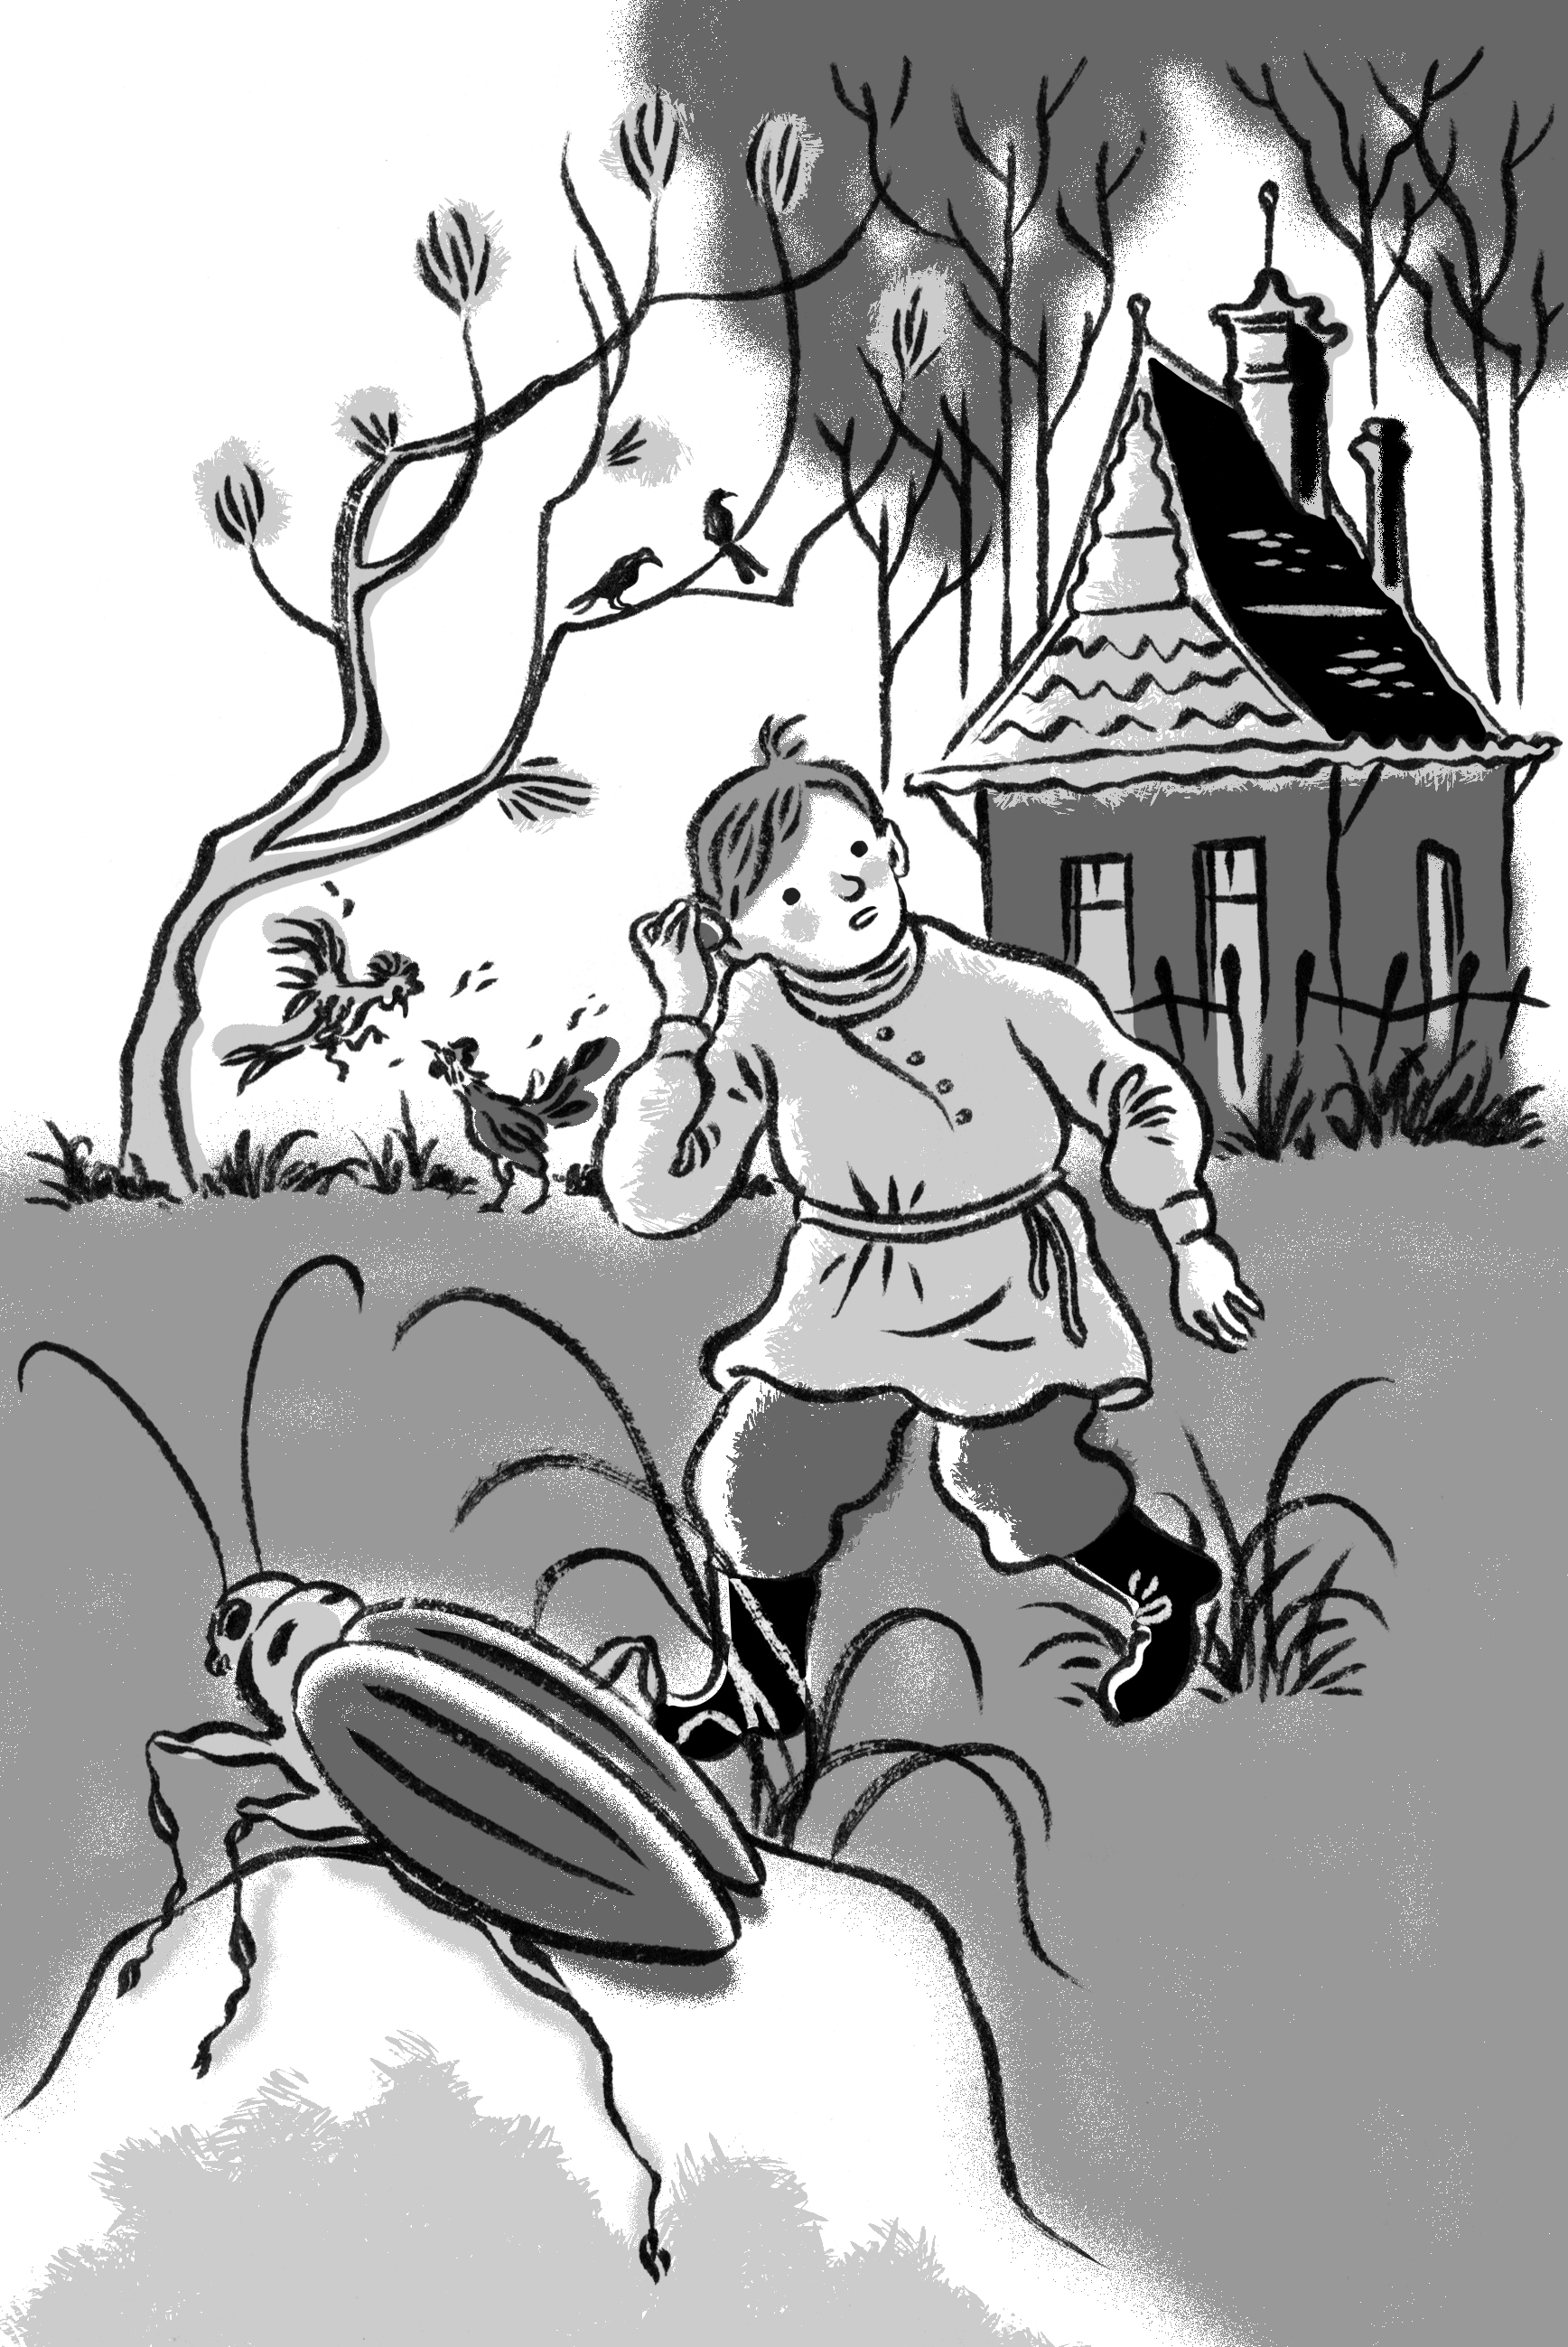
\includegraphics{./imgs/cena14.jpg}
\end{figure}

\medskip

{\footnotesize\hfill\emph{Tradução: Moissei Mountian}}


\chapter*{}
\label{part15}
\thispagestyle{empty}

\begin{vplace}[1.5]
{\HUGES\hfill\textbl{DANIIL KHARMS}}

{\LARGE\hfill\textlt(1905–1942)}
\end{vplace}

\pagebreak
\thispagestyle{empty}
\mbox{}
\vfill
\begin{center}
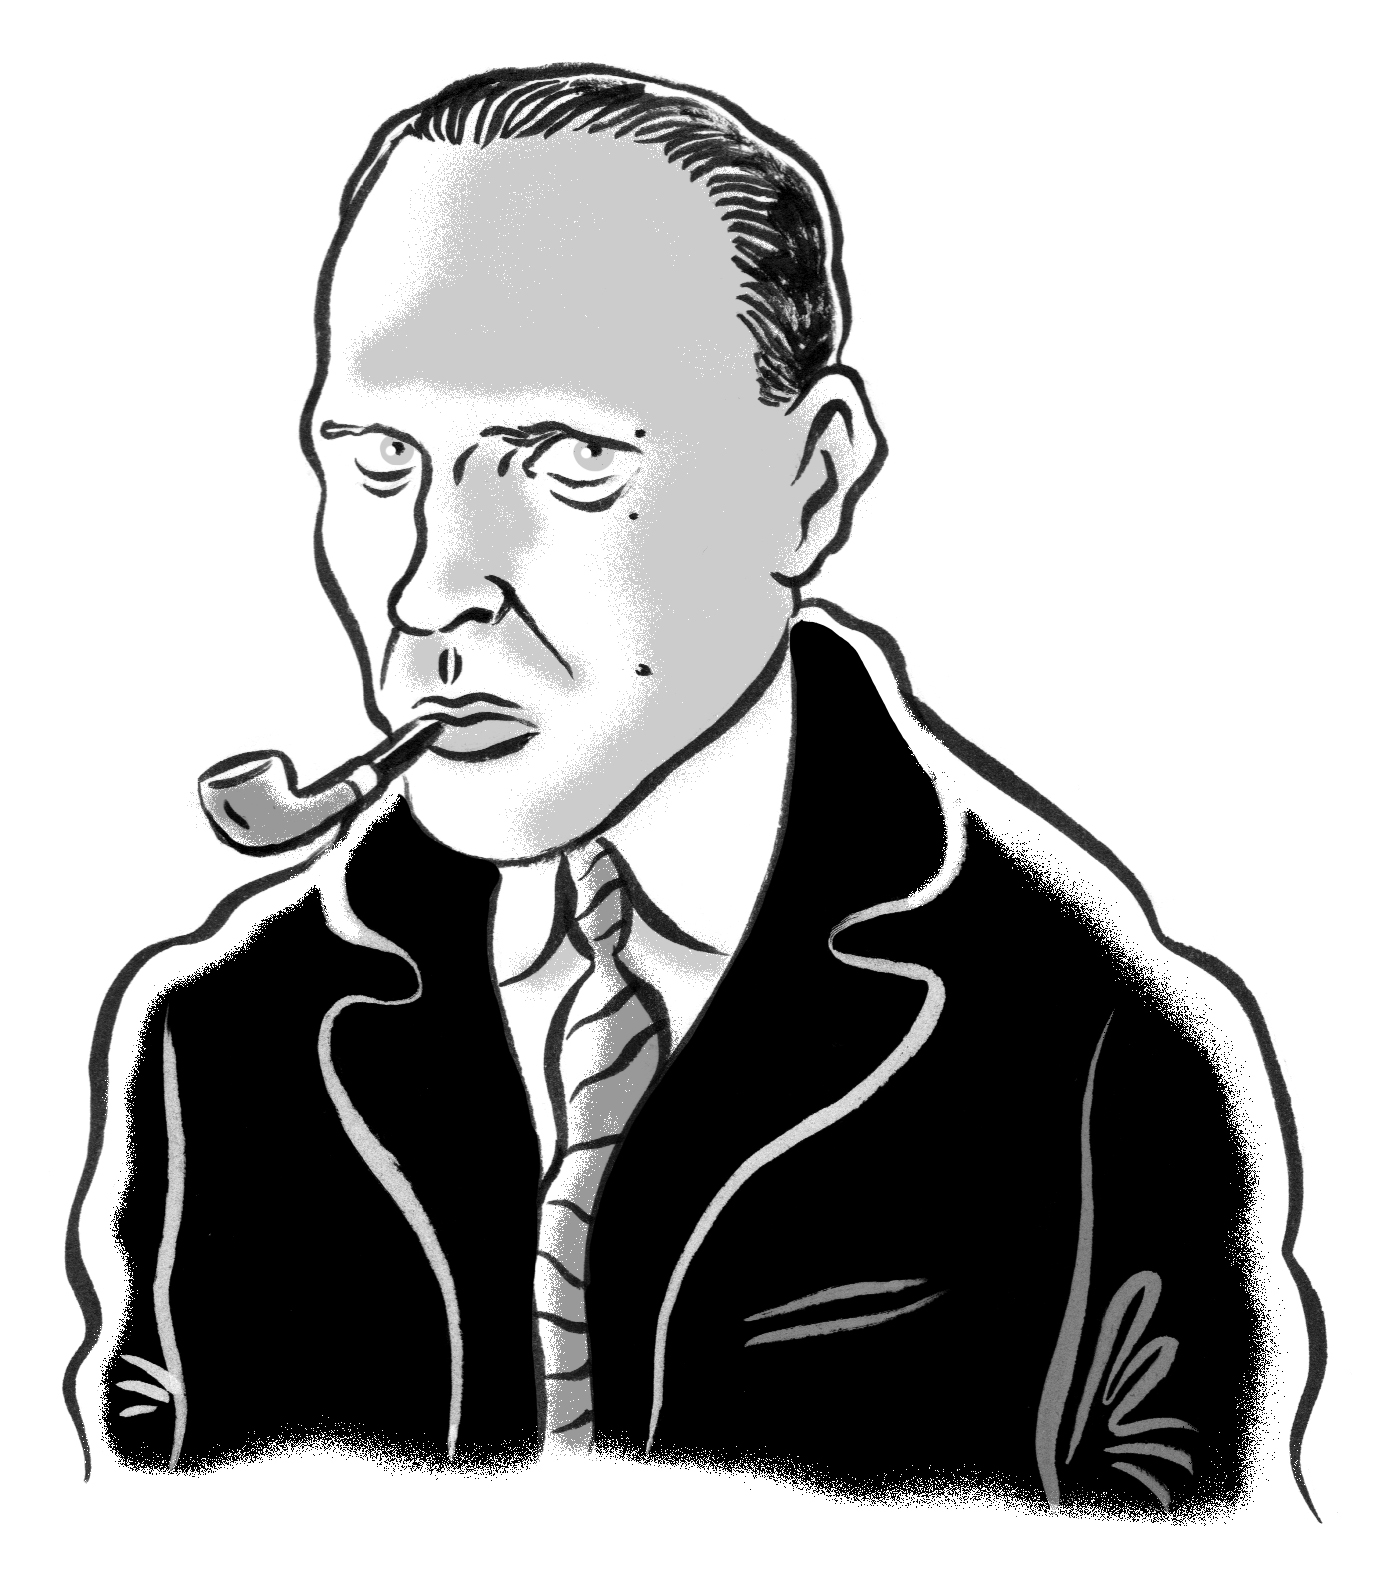
\includegraphics[width=6cm]{./imgs/autor12.jpg}
\end{center}

\chapter{Sobre como Kolka Pánkin viajou para\\ o Brasil e sobre como Pietka Erchóv\\ não acreditou em nada}

\section{1}

\noindent{}Kolka Pánkin decidiu fazer uma viagem a um lugar distante.

--- Vou para o Brasil --- disse ele a Pietka\footnote{Kolka é apelido de Nikolai e Pietka de Piotr.} Erchóv.

--- E onde fica esse tal Brasil? --- perguntou Pietka.

--- O Brasil fica na América do Sul --- disse Kolka ---, lá faz muito
calor, vivem macacos e papagaios, crescem palmeiras, voam colibris,
perambulam animais ferozes е habitam tribos selvagens.

--- Os índios? --- perguntou Pietka.

--- Algo do gênero --- disse Kolka.

--- E como se chega lá? --- perguntou Pietka.

--- De aeroplano ou de navio --- disse Kolka.

--- E você vai de quê? --- perguntou Pietka.

--- Vou de aeroplano --- disse Kolka.

--- E onde é que você vai arranjar um aeroplano? --- perguntou Pietka.

--- Vou até o aeródromo pedir um, e eles vão me dar --- disse Kolka.

--- E quem é que vai dar um aeroplano pra você? --- perguntou Pietka.

--- Eu conheço todo mundo lá --- disse Kolka.

--- E quem é que você conhece lá? --- perguntou Pietka.

--- Várias pessoas --- disse Kolka.

--- Você não tem conhecido nenhum lá --- disse Pietka.

--- Não, eu tenho! --- disse Kolka.

--- Não, não tem! --- disse Pietka.

--- Não, eu tenho!

--- Não, não tem!

--- Não, eu tenho!

--- Não, não tem!

Kolka Pánkin e Pietka Erchóv decidiram ir ao aeródromo na manhã
seguinte.

\section{2}

No dia seguinte, Kolka Pánkin e Pietka Erchóv saíram de casa bem
cedinho. Era longe para ir andando até o aeródromo, mas, como o tempo
estava bom e não tinham dinheiro para o bonde, Kolka e Pietka foram a
pé.

--- Vou para o Brasil de qualquer jeito --- disse Kolka.

--- E vai me escrever? --- perguntou Pietka.

--- Vou --- disse Kolka --- e, na volta, vou trazer um macaco pra você.

--- E um passarinho, vai trazer também? --- perguntou Pietka.

--- Vou trazer um passarinho --- disse Kolka ---, qual prefere: o
colibri ou o papagaio?

--- E qual é o melhor? --- perguntou Pietka.

--- O papagaio é o melhor, ele sabe falar --- disse Kolka.

--- E sabe cantar? --- perguntou Pietka.

--- Também sabe --- disse Kolka.

--- Com notas? --- perguntou Pietka.

--- Ele não sabe ler as notas. Mas é só cantar alguma coisa, que o
papagaio repete --- disse Kolka.

--- E vai mesmo me trazer um papagaio? ---perguntou Pietka.

--- Vou mesmo --- disse Kolka.

--- E se não trouxer? --- disse Pietka.

--- Se eu disse que trarei, então trarei --- disse Kolka.

--- Não, não trará! --- disse Pietka.

--- Sim, eu trarei! --- disse Kolka.

--- Não! --- disse Pietka.

--- Sim! --- disse Kolka.

--- Não!

--- Sim!

--- Não!

--- Sim!

--- Não!

Bem nesse momento Kolka Pánkin e Pietka Erchóv chegaram ao aeródromo.

\section{3}

Era tudo muito interessante no aeródromo. Os aeroplanos corriam pelo
solo, um atrás do outro, e então --- um, dois, três --- logo apareciam
no ar; no começo voavam baixinho, depois mais alto e mais alto, e
depois, dando um giro no ar, desapareciam por completo. Uns oito
aeroplanos ainda estavam no solo, também prontos para tomar impulso e
sair voando. Kolka Pánkin escolheu um deles e, apontando"-o a Pietka
Erchóv, disse:

--- É nesse aeroplano que eu vou para o Brasil.

Pietka tirou o boné e coçou a cabeça. Aí colocou o boné de volta e
perguntou:

--- E eles vão dar esse aeroplano pra você?

--- Vão --- disse Kolka ---, eu conheço um aviador lá.

--- Conhece? E qual é o nome dele? --- perguntou Pietka.

--- Muito simples: Pável Ivánovitch --- disse Kolka.

--- Pável Ivánovitch? --- repetiu Pietka.

--- Sim, sim --- disse Kolka.

--- E você vai pedir mesmo? --- perguntou Pietka.

--- Claro que vou. Venha comigo e verá --- disse Kolka.

--- E se ele não der o aeroplano? --- perguntou Pietka.

--- Mas como não? Eu vou pedir e ele vai dar --- disse Kolka.

--- E se você não pedir? --- perguntou Pietka.

--- Eu vou pedir --- disse Kolka.

--- Vai ficar com medo! --- disse Pietka.

--- Não, não vou ficar com medo --- disse Kolka.

--- É medroso! --- disse Pietka.

--- Não, não sou medroso! --- disse Kolka.

--- É medroso! --- disse Pietka.

--- Não, não sou medroso! --- disse Kolka.

--- É medroso!

--- Não, não sou medroso!

--- É medroso!

--- Não, não sou medroso!

Kolka Pánkin e Pietka Erchóv foram atrás do aviador.

\section{4}

O aviador estava perto do aeroplano limpando uns parafusinhos com a
gasolina que estava numa pequena bacia. Ele estava todo vestido de couro
e ao lado, no chão, estavam suas luvas de couro e seu capacete de couro.

Kolka Pánkin e Pietka Erchóv aproximaram"-se.

O aviador tirou os parafusos da gasolina, colocou"-os sobre a ponta da
asa do aeroplano, depois colocou outros parafusos na bacia e começou a
lavá"-los.

Kolka olhou, olhou, e disse:

--- Salve, Pável Ivánovitch.

O aviador olhou primeiro para Pietka, depois para Kolka e aí se virou de
novo. Kolka esperou, esperou, e disse outra vez:

--- Salve, Pável Ivánovitch.

Então o aviador olhou primeiro para Pietka, depois para Kolka e aí disse
coçando uma perna com a outra:

--- Eu não me chamo Pável Ivánovitch, mas Konstantin Konstantínovitch, e
não conheço nenhum Pável Ivánovitch.

Pietka tapou a boca para não rir e Kolka bateu nele. Pietka fez cara de
sério e Kolka disse ao aviador:

--- Konstantin Konstantínovitch, eu e Pietka Erchóv decidimos ir para o
Brasil, será que o senhor emprestaria seu aeroplano?

O aviador soltou uma gargalhada:

--- Quá"-quá"-quá, quá"-quá"-quá! E vocês estão seriamente decididos a ir
para o Brasil?

--- Sim --- disse Kolka.

--- O senhor irá conosco? --- perguntou Pietka.

--- E vocês realmente imaginaram --- gritou o aviador --- que eu daria a
máquina a troco de nada? Só podem estar brincando. Mas, se me pagassem,
eu poderia levar vocês até o Brasil. O que me dariam em troca?

Kolka vasculhou os bolsos, mas não achou nada.

--- Nós não temos dinheiro --- disse ele ao aviador ---, o senhor não
poderia nos levar assim mesmo?

\begin{figure}%[ht!]
\vspace*{-1.6cm}
\hspace*{-2.4cm}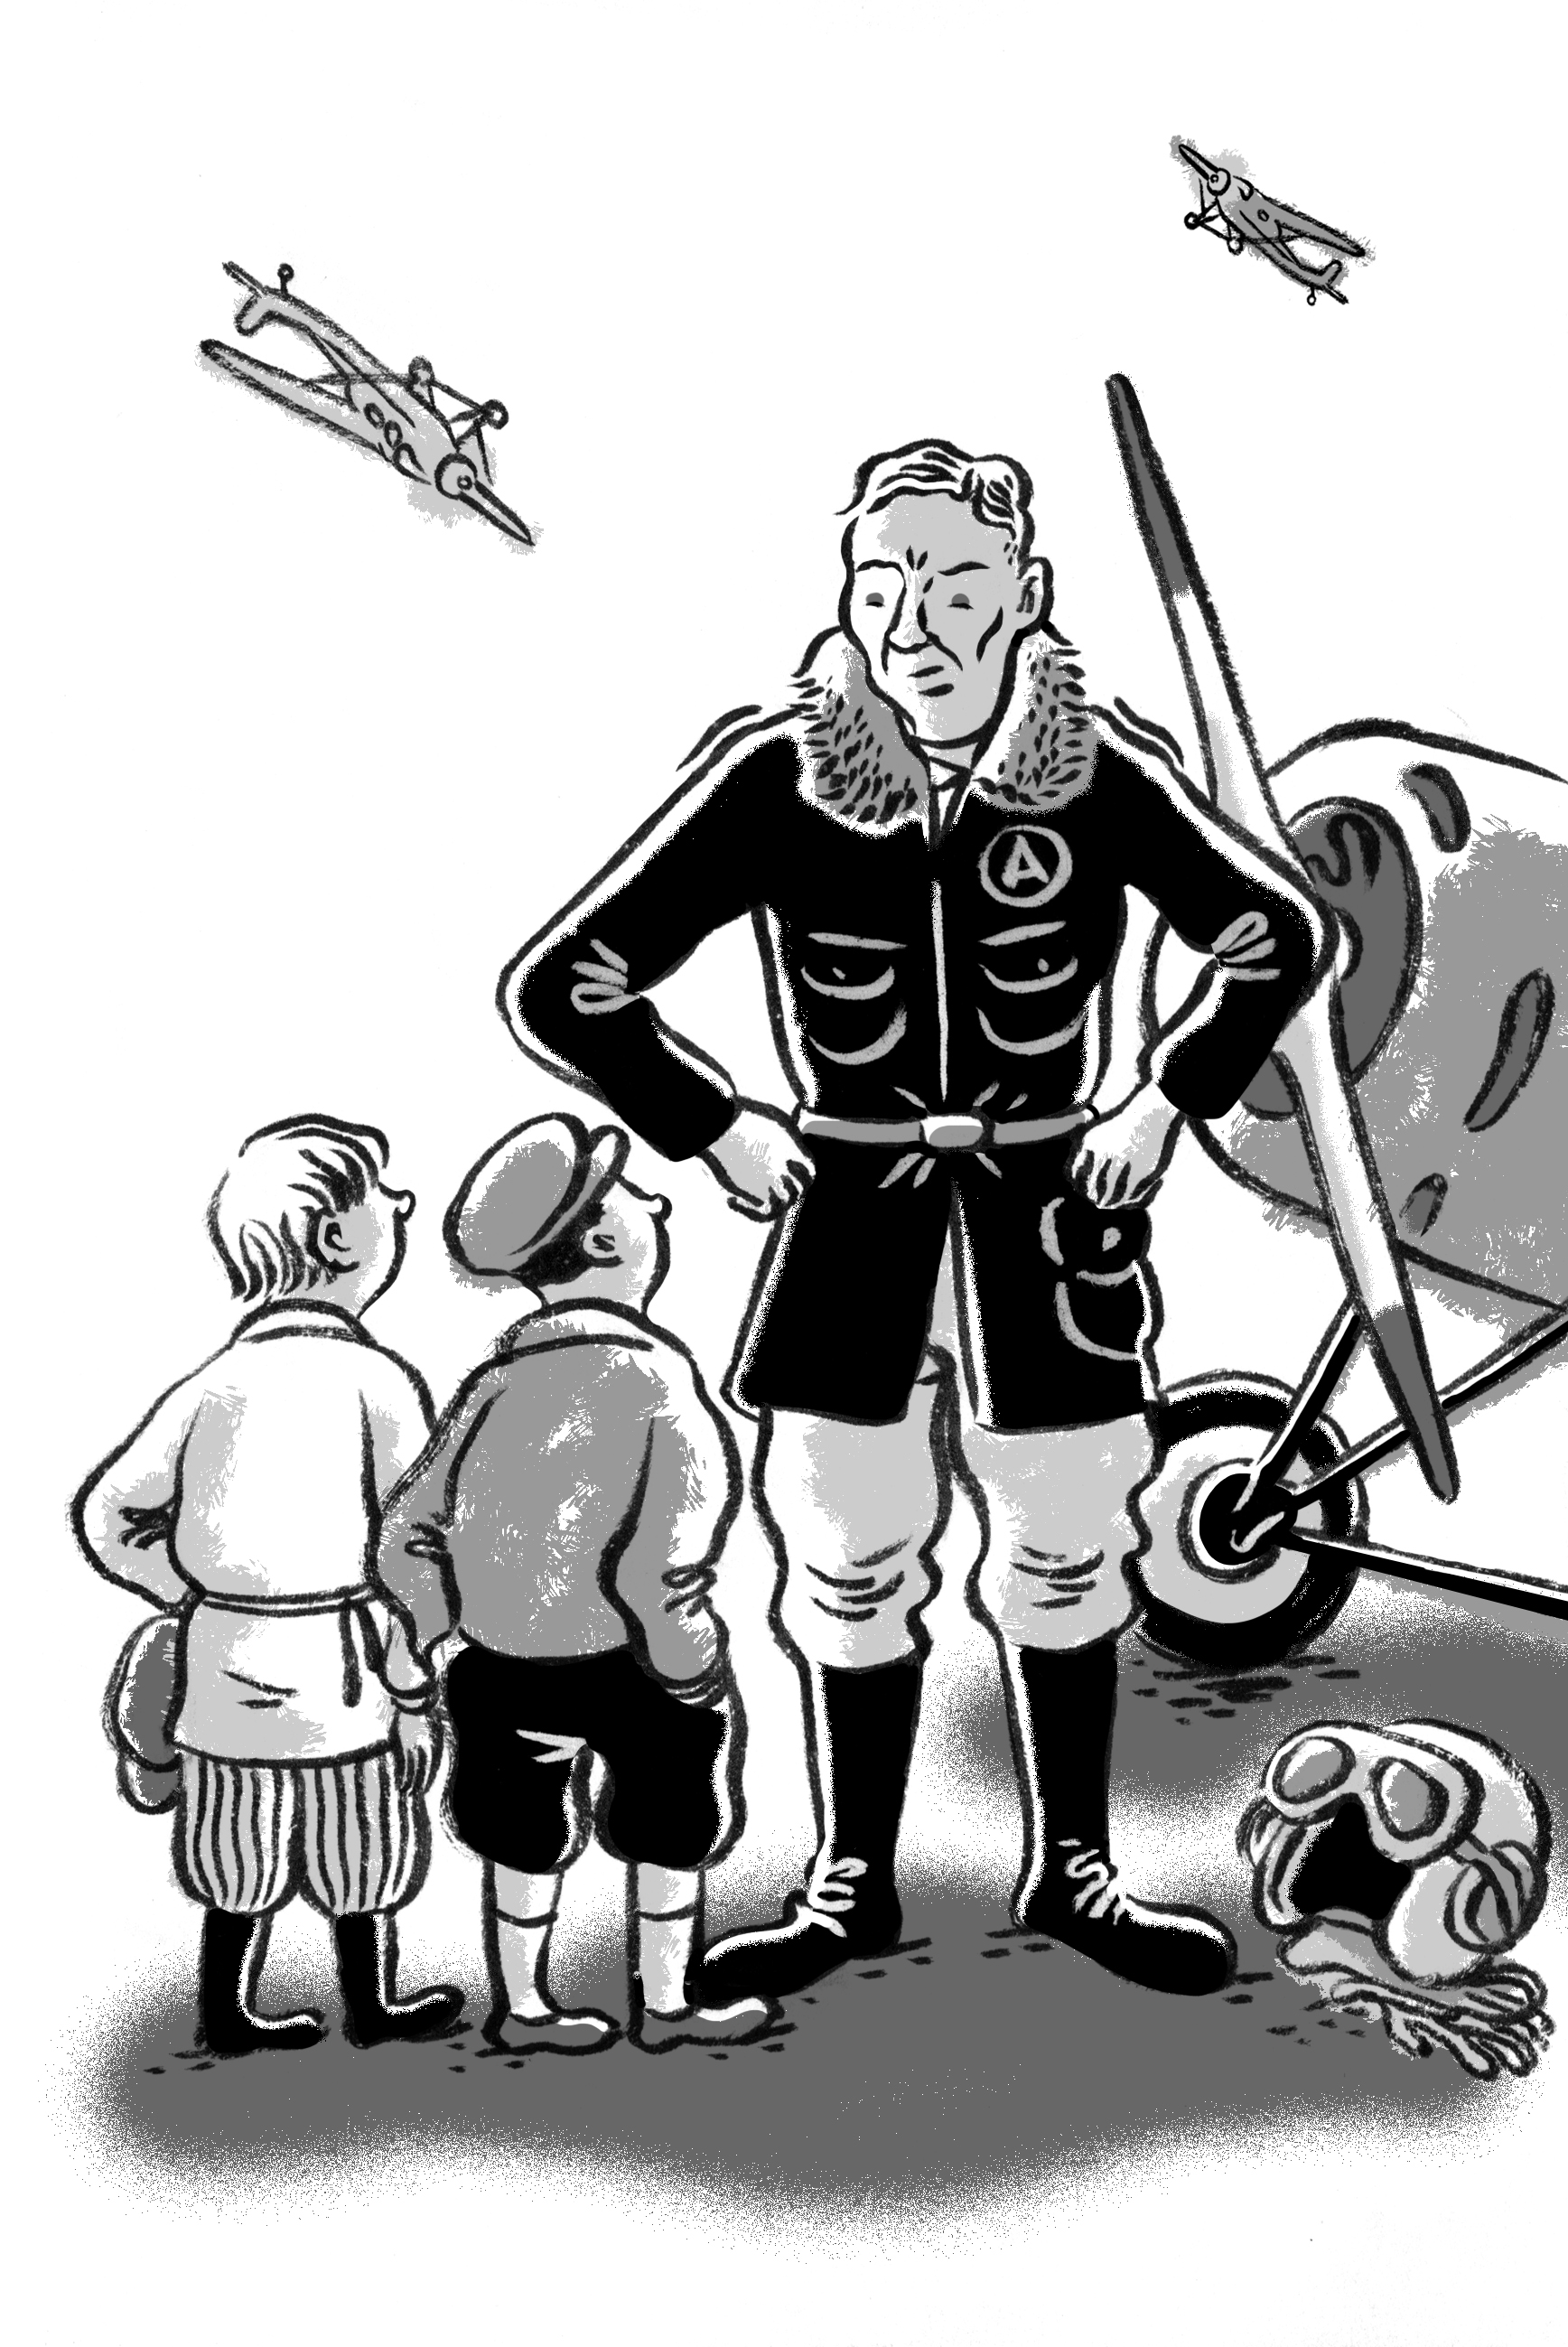
\includegraphics{./imgs/cena15.jpg}
\end{figure}

--- Não, assim eu não levo --- disse o aviador, e se virou para
consertar alguma coisa no aeroplano.

De repente Kolka agitou os braços e gritou:

--- Konstantin Konstantínovitch! Quer um canivete? Ele é muito bom, tem
três lâminas. Na verdade, duas estão quebra­das, em compensação uma está
inteirinha e é muito afiada. Uma vez eu dei um golpe na porta com o
canivete e ele atravessou a porta de lado a lado.

--- E quando foi isso? --- perguntou Pietka.

--- E o que você tem com isso? Foi no inverno! --- Kolka ficou zangado.

--- E que porta é essa? --- perguntou Pietka.

--- A da despensa --- disse Kolka.

--- Mas ela está inteirinha --- disse Pietka.

--- Então colocaram uma nova --- disse Kolka.

--- Não, não colocaram, é a velha --- disse Pietka.

--- Não, é uma nova --- disse Kolka.

--- E me devolva o canivete --- disse Pietka ---, este canivete é meu,
eu só emprestei pra você cortar a corda do varal e você nunca mais me
devolveu.

--- Como é que o canivete é seu? O canivete é meu --- disse Kolka.

--- Não, o canivete é meu! --- disse Pietka.

--- Não, é meu! --- disse Kolka.

--- Não, é meu! --- disse Pietka.

--- Não, é meu!

--- Não, é meu!

--- Com os diabos, já chega --- disse o aviador ---, sentem no
aeroplano, crianças, nós vamos ao Brasil.

\section{5}

Kolka Pánkin e Pietka Erchóv foram de aeroplano ao Brasil. E foi muito
interessante. O aviador ficou sentado no banco da frente e só dava para
ver seu capacete. Tudo estava muito bom. É verdade que o motor fazia
tanto barulho, que ficava difícil falar, mas, olhando para baixo, era
tudo tão amplo --- de perder o fôlego! E na terra era tudo tão pequeno e
parecia que uma coisa estava virada para outra do lado errado.

--- Piet"-ka! --- gritou Kolka ---, olhe que cidade toda tor"-ti"-nha!

--- O que"-e"-ê? --- gritou Pietka.

--- Ci"-da"-de! --- gritou Kolka.

--- Não ou"-ço! --- gritou Pietka.

--- O que"-e"-ê? --- gritou Kolka.

--- Falta muito para chegar ao Bra"-sil? --- gritou Pietka.

--- Que Ba"-sí"-lio? --- gritou Kolka.

--- O chapéu vo"-ou! --- gritou Pietka.

--- Quanto! --- grita Kolka.

--- On"-tem! --- grita Pietka.

--- América do Norte! --- grita Kolka.

--- Na"-vi"-da"-ri"-di"-i"-i! --- grita Pietka.

--- O quê? --- grita Kolka.

De repente, deu um vazio nos ouvidos e o aeroplano começou a descer.

\section{6}

O aeroplano saltou sobre algumas moitas e parou.

--- Chegamos --- disse o aviador.

Kolka Pánkin e Pietka Erchóv olharam ao redor.

--- Pietka --- disse Kolka ---, olhe só que Brasil!

--- E isto aqui é o Brasil? --- perguntou Pietka.

--- Seu tonto, será que você mesmo não vê? --- disse Kolka.

--- E quem são essas pessoas correndo? --- perguntou Pietka.

--- Onde? Ah, estou vendo --- disse Kolka. --- São os nativos, os
selvagens. Está vendo, as cabeças são brancas. Os penteados são feitos
de grama e palha.

--- Pra quê? --- perguntou Pietka.

--- É assim --- disse Kolka.

--- Pois eu acho que o cabelo deles é assim mesmo --- disse Pietka.

--- Mas estou dizendo que são penas --- disse Kolka.

--- Não, é cabelo! --- disse Pietka.

--- Não, penas! --- disse Kolka.

--- Não, cabelo!

--- Não, penas!

--- Não, cabelo!

--- Pois bem, desçam do aeroplano --- disse o aviador ---, eu preciso
voar.

\section{7}

Kolka Pánkin e Pietka Erchóv desceram do aeroplano e foram na direção
dos nativos. Os nativos eram baixos, sujos e de cabelos claros. Ao ver
Kolka e Pietka, eles pararam. Kolka deu um passo à frente,
levantou a mão direita e disse:

--- Oakh! --- disse na língua dos índios.

Os nativos ficaram boquiabertos e se calaram.

--- Gapakuk! --- disse Kolka.

--- O que você está dizendo? --- perguntou Pietka.

--- Estou conversando na língua dos índios --- disse Kolka.

--- E de onde você conhece a língua dos índios? --- perguntou Pietka.

--- Eu tinha um livrinho batuta e aprendi com ele --- disse Kolka.

--- Conte outra --- disse Pietka.

--- Não enche! --- disse Kolka. --- Inam kos! --- disse ele aos
nativos.

De repente os nativos deram uma risada.

--- Kerek eri iale --- disseram os nativos.

--- Ara toki --- disse Kolka.

--- Mita? --- perguntaram os nativos.

--- Pare com isso, vamos embora --- disse Pietka.

--- Pilguedrau! --- gritou Kolka.

--- Perkilia! --- gritaram os nativos.

--- Kulmeguinki! --- gritou Kolka.

--- Perkilia, perkilia! --- gritaram os nativos.

--- Vamos dar no pé! --- gritou Pietka ---, eles querem é brigar.

Mas já era tarde. Os nativos atiraram"-se contra Kolka e começaram a
bater nele.

--- Socorro! --- gritou Kolka.

--- Perkilia! --- gritaram os nativos.

``Mm"-uuu'', uma vaca mugiu.

\section{8}

Depois de baterem em Kolka para valer, os nativos fugiram atirando terra
no ar. Kolka ficou ali desgrenhado e todo amarrotado.

--- Pie"-pie"-pie"-pie"-pietka --- disse ele com a voz trêmula. --- Que
surra que eu dei nesses nati"-ti"-ti"-vos. Um pa"-pa"-pa"-para cá, outro
pa"-pa"-pa"-para lá.

--- E eles, por acaso não bateram em você? --- perguntou Pietka.

--- Que bobagem! --- disse Kolka. --- Fui eu que peguei todos eles:
um"-dois, um"-dois, um"-dois!

``Mm"-uuu'', soou nos ouvidos de Kolka.

--- Ai! --- Kolka gritou e correu.

--- Kolka. Ko"-olka"-a"-a! --- gritava Pietka.

Mas Kolka corria sem olhar para trás.

Correram, correram,

correram, correram,

correram, correram,

e, só quando chegaram à floresta, Kolka parou.

--- Ufa! --- disse ele, retomando o fôlego.

Pietka ficou tão ofegante com a corrida que não conseguiu dizer nada.

--- Mas que bisonte! --- disse Kolka depois de retomar o fôlego.

--- Quê? --- perguntou Pietka.

--- Não viu o bisonte? --- perguntou Kolka.

--- Onde? --- perguntou Pietka.

--- Bem ali. Ele se atirou na gente --- disse Kolka.

--- Não era uma vaca? --- perguntou Pietka.

--- Que bobagem! Que espécie de vaca é essa? Não existem vacas no Brasil
--- disse Kolka.

--- E será que bisontes andam com sininhos no pescoço? --- perguntou
Pietka.

--- Andam --- disse Kolka.

--- De onde vêm os sininhos? --- perguntou Pietka.

--- Dos índios. Toda vez que os índios capturam um bisonte, eles amarram
um sininho nele e depois soltam o bicho.

--- Pra quê? --- perguntou Pietka.

--- É assim --- disse Kolka.

--- Não é verdade, bisontes não andam com sininhos, e aquilo era uma
vaca --- disse Pietka.

--- Não, um bisonte! --- disse Kolka.

--- Não, uma vaca! --- disse Pietka.

--- Não, um bisonte!

--- Não, uma vaca!

--- Não, um bisonte!

--- E cadê os papagaios? --- perguntou Pietka.

\section{9}

Kolka Pánkin ficou todo confuso na hora.

--- Que papagaios? --- perguntou a Pietka Erchóv.

--- Sim, você prometeu pegar uns papagaios assim que a gente chegasse.
Se isto aqui é o Brasil, então cadê os papagaios? --- disse Pietka.

--- Não dá pra ver os papagaios, em compensação os colibris estão
sentados logo ali --- disse Kolka.

--- Ali no pinheiro? --- perguntou Pietka.

--- Isso não é um pinheiro, é uma palmeira --- ofendeu"-se Kolka.

--- Mas nos desenhos as palmeiras são diferentes --- disse Pietka.

--- Nos desenhos são outras palmeiras, no Brasil elas são assim ---
zangou"-se Kolka. --- Olhe, cada colibri!

--- Parecem os nossos pardais --- disse Pietka.

--- Parecem --- concordou Kolka ---, mas são menores.

--- Não, maiores! --- disse Pietka.

--- Não, menores! --- disse Kolka.

--- Não, maiores! --- disse Pietka.

--- Não, menores! --- disse Kolka.

--- Não, maiores!

--- Não, menores!

--- Não, maiores!

--- Não, menores!

De repente, ouviu"-se um barulho atrás de Kolka e Pietka.

\section{10}

Kolka Pánkin e Pietka Erchóv viraram"-se. Uma espécie de monstro voava na
direção deles.

--- O que é isto? --- assustou"-se Kolka.

--- É um automóvel --- disse Pietka.

--- Não pode ser! --- disse Kolka. --- Como um automóvel foi parar no
Brasil?

--- Não sei --- disse Pietka ---, só sei que é um automóvel.

--- Não pode ser! --- disse Kolka.

--- Estou dizendo que é um automóvel --- disse Pietka.

--- Não, não pode ser --- disse Kolka.

--- Não, pode!

--- Não, não pode!

--- Então, agora está vendo que é um automóvel mesmo? --- perguntou
Pietka.

--- Estou vendo, mas é muito estranho --- disse Kolka.

Nesse meio"-tempo, o automóvel se aproximou.

--- Ei, crianças --- gritou um homem de dentro do automóvel. --- A
estrada para Leningrado é a da esquerda ou a da direita?

--- Para qual Leningrado? --- perguntou Kolka.

--- Como para qual? Então, como faço para chegar até a cidade? ---
perguntou o motorista.

--- Nós não sabemos --- disse Pietka e, de repente, deu de chorar.

--- Tiozinho --- dizia ele chorando ---, leve a gente para a cidade.

--- Mas vocês são da cidade mesmo? --- perguntou o motorista.

--- Sim --- chorava Pietka ---, da Rua Mokhovaia.

--- E como vieram parar aqui? --- surpreendeu"-se o motorista.

--- É que o Kolka --- chorava Pietka --- tinha prometido me levar até o
Brasil, mas me trouxe pra cá.

--- Para Brussílovo\ldots{} Brussílovo\ldots{} Esperem, Brussílovo é mais pra lá,
é perto da província de Tchernígov --- disse o motorista.

--- Província de Chilígov\ldots{} República de Chilínskie\ldots{} Chile\ldots{} É mais
para o sul, lá onde fica a Argentina. Chile fica à margem do Oceano
Pacífico --- disse Kolka.

--- Tiozinho --- Pietka choramingou de novo ---, leve a gente para casa.

--- Está bem, está bem --- disse o motorista. --- Sentem aí, o carro
está vazio de qualquer jeito. Só que Brussílovo não fica aqui,
Brussílovo fica na província de Tchernígov.

Então Kolka Pánkin e Pietka Erchóv foram para casa de automóvel.

\section{11}

No começo, Kolka Pánkin e Pietka Erchóv foram em silêncio. Depois Kolka
olhou para Pietka e disse:

--- Pietka --- disse Kolka ---, você já viu um condor?

--- Não --- disse Pietka. --- O que é isso?

--- É um pássaro --- disse Kolka.

--- Grande? --- perguntou Pietka.

--- Muito grande --- disse Kolka.

--- Maior do que o corvo? --- perguntou Pietka.

--- Que bobagem! É o maior pássaro que existe --- disse Kolka.

--- Mas eu nunca vi --- disse Pietka.

--- Mas eu já. Ele estava sentado numa palmeira --- disse Kolka.

--- Em qual palmeira? --- perguntou Pietka.

--- Na palmeira onde estava o colibri --- disse Kolka.

--- Aquilo não era uma palmeira, era um pinheiro --- disse Pietka.

--- Não, uma palmeira! --- disse Kolka.

--- Não, um pinheiro! --- disse Pietka. --- Palmeiras só crescem no
Brasil, aqui não crescem palmeiras.

--- Mas nós fomos para o Brasil --- disse Kolka.

--- Não, não fomos! --- disse Pietka.

--- Não, fomos! --- disse Kolka.

--- Não"-fo"-mos! --- gritou Pietka.

--- Fomos, fomos, fomos, fo"-mo"-o"-os! --- gritou Kolka.

--- Lá está Leningrado --- disse o motorista apontando para os telhados
e para as chaminés que espetavam o céu.

\bigskip

\begin{center}
\textsc{assim é que é.}
\end{center}

\hfill\emph{Daniil Kharms}

\hfill\emph{1928}

\medskip

{\footnotesize\hfill\emph{Tradução Moissei Mountian.}}
